\documentclass[11pt,a4paper,twoside]{book}
\usepackage{fontenc}[T1]
\usepackage[utf8]{inputenc}
\usepackage[english]{babel}
\usepackage{amssymb,amsmath}
\usepackage[top=2cm,bottom=2cm,left=2cm,right=2cm]{geometry}
\usepackage[pdftex]{graphicx} %per poter inserire le figure
\usepackage{amssymb,amsmath,amsthm,amsfonts}
\usepackage{xspace}
\usepackage{tabularx}
\usepackage{indentfirst}
\usepackage{subfigure}
\usepackage[small]{caption}
\usepackage{eucal}
\usepackage{eso-pic}
\usepackage{url}
\usepackage{booktabs}
\usepackage{afterpage}
%\usepackage{parskip}
\usepackage{listings}
\usepackage{fancyhdr}
\usepackage{textcomp}
\usepackage{cite}
\usepackage{multirow}
\usepackage[utf8]{inputenc}   %per riuscire a scrivere gli accenti
\usepackage{setspace}
\usepackage{fancyhdr}
\newenvironment{abstract}{\cleardoublepage\thispagestyle{empty}\null\vfill\begin{center}\bfseries\abstractname\end{center}}{\vfill\null}
\pagestyle{fancy} 


\begin{document}
	\frontmatter
	\begin{titlepage}
		\vspace{5mm}
		\begin{figure}[hbtp]
			\centering
			
\includegraphics[scale=.16]{Logo_unipd.png}
		\end{figure}
		\vspace{5mm}
		\begin{center}
			{{\huge{\textsc{\bf UNIVERSIT\`A DEGLI STUDI DI PADOVA}}}\\}
			\vspace{5mm}
			{\Large{\bf Dipartimento di Fisica e Astronomia ``Galileo Galilei''}} \\
			\vspace{5mm}
			{\Large{\textsc{\bf Master Degree in Physics}}}\\
			\vspace{20mm}
			{\Large{\textsc{\bf Final Dissertation}}}\\
			\vspace{30mm}
			\begin{spacing}{3}
				{\LARGE \textbf{Probing the Reheating Phase After Inflation}}\\
			\end{spacing}
			\vspace{8mm}
		\end{center}
		
		\vspace{20mm}
		\begin{spacing}{2}
			\begin{tabular}{ l  c  c c c  cc c c c c  l }
				{\Large{\bf Supervisor}} &&&&&&&&&&& {\Large{\bf Candidate}}\\
				{\Large{\bf Prof. Nicola Bartolo}} &&&&&&&&&&& {\Large{\bf Raffaele Giusti}}\\
			\end{tabular}
		\end{spacing}
		\vspace{15 mm}
		
		\begin{center}
			{\Large{\bf Academic Year 2021/2022}}
		\end{center}
	\end{titlepage}
	\clearpage{\pagestyle{empty}\cleardoublepage}

\begin{abstract}
	Inflation is the standard scenario, completely consistent with a variety of data, to understand the  
	generation of primordial scalar (density) perturbations, i.e.  the seeds of all the cosmological structures we  
	see today, and also of tensor perturbations (i.e. primordial gravitational waves). Inflation must come to an  
	end, in order for the universe to be filled in with radiation, and to proceed  through the standard radiation  
	dominated era, during which, e.g. primordial nucleosynthesis can take place. Such a transition (called  
	reheating phase) from the inflationary stage to the standard radiation dominated epoch, is the least known  
	part of the inflationary scenario, because, e.g., it involves couplings of the fields driving inflation to other  
	(relativistic) particles.  	
	Nonetheless the precision of cosmological data has allowed recently to put already some constraints on  
	such a reheating phase.  
	
	This Thesis will provide an up-to-date review of all the cosmological observables that can be used to open  
	a new window into such period of the early universe. 	
	Moreover, we will also review the main models present in the literature about the preheating epoch (the initial stage of reheating) and the subsequent phases of reheating. These stages involve very non-linear and interesting physics and can lead to production of gravitational waves that can be observed today.
\end{abstract}
	
\tableofcontents
	

\chapter{Introduction}
\markboth{INTRODUCTION}{INTRODUCTION}

In modern cosmology one of the most important theories is represented by \textit{Cosmological Inflation}. 

Inflation was an era during the early history of the universe, before the epoch of primordial nucleosynthesis, during which the universe expansion was accelerated. Such a period can be attained if the energy density of the universe was dominated by the vacuum energy density associated with the potential of a scalar field, called the \textit{inflaton field} $ \phi $. 

Inflation leads to a very rapid expansion of the universe and can elegantly solve the flatness, the horizon and the monopole problems of the Standard Big Bang Cosmology (the first important model of inflation by Guth in 1981 was introduced to address such problems \cite{Guth:Intro}). It can explain the production of the first density perturbations in the early universe, which are the seeds for the Large Scale Structure (LSS) in the distribution of galaxies and underlying dark matter, and for the Cosmic Microwave Background (CMB) temperature anisotropies that we observe today. Inflation has become the dominant paradigm to understand the initial conditions for structure formation and CMB anisotropies.
During this era primordial density fluctuations and gravitational waves are created from quantum fluctuations \textquotedblleft redshifted" out of the horizon during the rapid expansion and here \textquotedblleft frozen\textquotedblright.

 From this period we can observe temperature anisotropies in the CMB caused by perturbations at the surface of the last scattering. The CMB temperature anisotropies were first detected by the Cosmic Background Explorer (COBE) satellite \cite{COBE1:intro},\cite{COBE2:intro}. 
Another impressive confirmation of the inflationary theory has been provided by the data of the Wilkinson Microwave Anisotropy Probe (WMAP) mission, that has produced a full-sky map of the angular variations of the CMB with unprecedented accuracy. WMAP data confirm the inflationary mechanism as responsible for the generation of super-horizon fluctuations \cite{WMAP:intro}, \cite{NonGauss:Intro}.
More recently, the best constraints on the CMB data are provided by the \textit{2018 Planck measurements} \cite{Planck2018:intro}. The \textit{Planck} data have given a very precise characteritation of the primordial cosmological perturbations and have allowed cosmological parameters to be constrained at the sub-percent level. Thus, \textit{Planck} measurements provide  a powerful constraint to inflationary models \cite{Planck2013:Intro}. In particular, the \textit{Planck} data have established with extremely high precision (at more than 8 sigma) that the primordial density perturbations are not scale-invariant, which is another generic prediction of inflation; also, the \textit{Planck} data have provided one of the most stringest test on inflationary models by providing the strongest constraints on deviations from Gaussianity of the cosmological perturbations.

The literature contains a huge number of different models of inflation. Each model amounts to a choice for the potential  of the inflaton. In the simplest scenario, the main models of inflation focuse on two different paradigms. Throughout the early 1990s discussion was dominated by the \textit{single-field models}. In these models the scalar field potential often is chosen to be some convenient simple function, such as a monomial or exponential, and the initial conditions are chosen such that the scalar field is well displaced from any minimum.

In the mid-1990s this paradigm was challenged by a new wave of inflationary model building, based on particle physics motivation such as the theories of supersymmetry, supergravity, and superstrings. In such a period we have a new class of models, known generically as \textit{hybrid inflation} models, which rely on interactions between two scalar fields and exploit the flat potentials expected in supersymmetry theories \cite{Liddle:intro}. 
In other scenarios we have the presence of a further scalar field besides the inflaton that does not influence the inflationary dynamics (for example the \textit{curvaton scenario}), or the inflaton coupled to a gauge field. Finally, there are theories based on Modified Gravity (MG) that involve a modification of General Relativity \cite{GWFromInflation:Intro}.

Inflation cannot proceed forever. In fact, the greatest successes of the Standard Big Bang model, such as primordial nucleosynthesis and the origin of the CMB, require the standard evolution from radiation to matter dominated era.
The transition from inflation to later stages of the evolution of the universe (radiation and matter dominance) is referred to as \textit{Reheating}. In the simplest models (single-field, slow-roll scenario) inflation ends when the inflaton field starts rolling fast along its potential, it reaches the minimun and then oscillates around it. During reheating the inflaton loses its energy, eventually leading to the production of ordinary matter.
 More intricate scenarios include non perturbative processes such as (broad) resonance decay, tachyonic instability, instant preheating, fermionic preheating. \textit{Preheating} denotes the initial stage of reheating where we have an exponential decay that generates high occupation numbers in selected frequency bands.  
 
 The aim of this Thesis is to provide a complete and up-to-date review of the main models of reheating discussed in the literature.
However, the reheating era is difficult to constrain observationally. In the absence of topological defects like monopoles or strings, the fluctuations produced during reheating remain sub-horizon and cannot leave an observable imprint at the level of the CMB or LSS. A lower bound is placed on the reheating temperature (i.e. the temperature at which the standard radiation era of the universe begins after reheating) by primordial nucleosynthesis (BBN) $ T_{BBN} \sim  10^{-2} Gev $ \cite{Steigman:nucleosynthesisIntro}. The scale of inflation is bounded from above and can be as large as $ \sim 10^{16} Gev $, leaving for the reheating temperature an allowed range of many orders of magnitude. 
Moreover, a variety of signatures relative to production of primordial black holes, magnetic fields, unwanted relics, and also to mechanisms such as baryo  and leptogenesis, may be traced back to specific preheating/reheating models \cite{ReheatingPredictionsSingleFieldModel:intro}.

An extremely important prediction of cosmological inflation is the generation of a Stochastic Background of primordial Gravitational Waves (SGWB). Primordial GW are in fact not expected in the non-inflationary standard early universe models and will provide, if detected, a \textit{smoking gun} probe of inflation. In the standard slow-roll inflationary scenario tensor fluctuations of the metric (i.e. primordial GW) are characterized by a nearly scale invariant spectrum on super-horizon scales. The amplitude of the GW signal is usually described by the tensor-to-scalar ratio \textit{r}, defined as the ratio between the tensor and the scalar power spectrum amplitudes at a given pivot scale $ k_{*} $.
The current best bound on $ \textit{r} $ comes from the joint analysis of \textit{Planck} and BICEP/Keck 2018, which yields $ r < 0.032 $ at $ 95 \% $ C.L. for $ k_{*}$ = $ 0.05\ Mpc^{-1} $ \cite{Intro:ConstraintsOnr}. 
A crucial point is that, even in the simplest single field framework, different inflationary scenarios predict different values of $r$. The study of observational signatures of primordial GW thus provides not only a way to probe the general inflationary theory, but also to discriminate in detail among specific models.

A detection of primordial GW would not only be extremely important for Cosmology, but also for High Energy and Fundamental Physics. Since the energy scale of inflation is directly linked to the value of the tensor-to-scalar ratio, by means of a detection of $ r $ we would obtain a hint of the the physics beyond the Standard Model of Particle Physics and the precise indication of the energy regime of such new physics.
Indeed, the primordial GW are the object of a growing experimental effort, and their detection will be a major goal for Cosmology in the forthcoming  decades. 

The main observational signature of the inflationary GW background is a curl-like pattern (B-mode) in the CMB. A number of, present or forthcoming, ground-based or baloon-borne experiments, are specifically aimed to B-mode detection. Unfortunately, the B-modes measured by BICEP2 \cite{Bicep2BMode:Intro} did not point to any inflationary signal, but several next-generation CMB space missions have been proposed in recent years with the specific goal of B-mode detection such as COrE \cite{COre:intro} or PRISM \cite{PRISM:intro}, and more recently LiteBIRD (https://www.isas.jaxa.jp/en/missions/spacecraft/future/litebird.html). 
Finally, we have the possibility of a future direct detection, by experiments such as aLIGO \cite{LIGO:intro}, or eLISA \cite{Lisa:Intro}, especially if some inflationary models produced a blue-tilted primordial tensor spectrum \cite{GWFromInflation:Intro}.

In this thesis we will focus also on another type of GW: those generated by classical mechanisms during reheating after inflation. By investigating  GW we cannot neglect this stage. In fact, there are many models for the reheating period which provide further GW production, besides the inflationary stage. Moreover, it can be shown that reheating parameters are related to inflationary power-spectra ones, so that the constraints on tensor perturbations are related to those on the reheating period.


In this work we are going to review all the most important inflation and reheating scenarios. After the first three chapters we will present detailed models of reheating about each of its stages (Preheating, Bubbly Stage, Scalar Wave Turbolence, Thermalization) investigated in the literature. Moreover, we will review predictions about the production of GW, observable signatures on CMB and the possibility of direct detection of GW from reheating epoch.

The Thesis is organized with the following plan:\\
In  chapter 1 we review the standard single-field model of slow-roll inflation and we derive some of the physical observables that can be seen and constrained from CMB. 

In chapter 2 we overview the main inflationary models and a simple toy model of reheating is presented.

 In chapter 3 we explain  how gravitational waves can put some constraints about the reheating epoch. Moreover, we derive some quantities important for such  a stage coming from CMB observables.
 
In  chapter 4, we investigate about \textit{preheating}, the first stage of reheating, exploiting the main models discussed in the literature. 

In  chapter 5 we examinate the non-linear stage at the end of preheating. This stage is extremely non-linear and complicated. In this chapter we show some lattice simulations performed in the literature.

In  chapter 6 we discuss the turbolent  and Thermalization stage after preheating.

In chapter 7 we present the results found in the literature about the gravitational waves generated during the reheating stage. 

In the conclusions we summarise the main points and the results of the thesis.

 
 \mainmatter
 
\chapter{Inflation}

The inflation theory not only provides an excellent way to solve flatness and horizon problems, but also generates density perturbations as seeds for the large-scale structure in the universe. Quantum fluctuations of the field that drives inflation (called \textit{inflaton}) are streched on large scales by the accelerated expansion. In the simplest version of the single-field scenario the fluctuations are \textquotedblleft frozen" after the scale of perturbations leaves the Hubble radius during inflation. Long after inflation ends, the perturbations cross inside the Hubble radius again. Thus, inflation provides a mechanism for the origin of the large-scale structures in the universe. An important prediction of inflation is that density perturbations generally exhibit a tiny deviation from scale-invariance. This prediction can be directly tested by the measurement of the temperature anisotropies in the Cosmic Microwave Background (CMB). All data acquired until now have continued to confirm the main predictions of the inflationary theory within observational errors \cite{InflationDynamicsAndReheating:chap1}.

In this first chapter we review the simple standard model of slow-roll inflation and we derive observables and relations that will be used in the next chapters.

\section{Standard Big-Bang Cosmology}

The Standard Big-Bang Cosmology is based upon the cosmological principle which requires that the universe is homogeneous and isotropic on averaging over large volumes. 

A homogeneous and isotropic universe is described by the Friedmann-Robertson-Walker metric (FRW):

\begin{equation}
	\label{metric}	
	ds^{2}   = - dt^{2} + a^{2}(t)\Big[\frac{dr^{2}}{1-Kr^{2}}  +  r^{2}(d\theta^{2} + \sin^{2} \theta d\phi^{2})\Big] . 
\end{equation}
Here $a(t)$ is the scale factor with $ t $ being the cosmic time and $(r,\theta,\phi) $ are comoving (spherical) coordinates. The constant $ K $ is the spatial curvature where positive, zero, and negative values correspond to closed, flat, and hyperbolic spatial sections, respectevely. 

The evolution of the universe is dependent on the material within it. A key role is played by the \textit{equation of state} relating the energy density $ \rho (t) $ and the pressure $ P(t) $. Assuming a perfect and barotropic fluid, we can describe it with the relation $ P=\omega\rho $, with $ \omega=0 $ for non-relativistic matter (dust) and $ \omega=1/3 $ for radiation.
For example, in the universe we have $ P=0 $ or $ P=1/3 $ if it is dominated by dust or radiation, respectevely. 

The dynamical evolution of the universe is known once we solve the Einstein equations of General Relativity:
\begin{equation}
	\label{eq:gr}
	G_{\mu\nu}  = R_{\mu\nu} - \frac{1}{2}g_{\mu\nu}R=8\pi G T_{\mu\nu},
\end{equation}
where $ G_{\mu\nu} $ is the Einstein Tensor, $ R_{\mu\nu} $, $ R $, $ T_{\mu\nu}$ and G are the Ricci tensor, Ricci scalar, energy-momentum tensor and gravitational constant, respectively. The energy-momentum tensor $ T_{\mu\nu} $ describes the perfect fluid with density energy $ \rho $ and isotropic pressure P that fills the universe.
The Planck energy, $M_{pl}=1.2211 \times 10^{19}$ GeV, is related to G through the relation $ M_{pl} = (\hslash c^{5}/G)^{1/2}$. Hereafter we use the units $ \hslash = c = 1 $.

From the Einstein equations (\ref{eq:gr}) for the background FRW metric (\ref{metric}) we obtain the Friedmann equations:
\begin{equation}
	\label{friedmannEquations1}
	H^{2}=\frac{8\pi G}{3}\rho - \frac{K}{a^{2}},
\end{equation}
\begin{equation}
	\label{friedmannEquations2}	
	\frac{\ddot{a}}{a} = -\frac{4\pi G}{3}(\rho + 3P),
\end{equation}
where the dots denote the derivative with respect to t, and $ H=\dot{a}/a $ is the Hubble expansion rate. Combining these relations we obtain the energy conservation equation 
\begin{equation}
	\label{energyCons}
	\dot{\rho} + 3H(\rho + P)=0,
\end{equation}
which is known as the continuity or fluid equation.

The Friedmann equation (\ref{friedmannEquations1}) can be rewritten as 
\begin{equation}
	\label{densityParameter}
	\Omega - 1 = \frac{K}{a^{2}H^{2}},
\end{equation}
with 
\begin{equation}
	\label{criticalDensity}
	\Omega=\frac{\rho}{\rho_{c}}, \quad     \quad   \rho_{c}=\frac{3H^{2}}{8\pi G},
\end{equation}
where the density parameter $ \Omega $ is the ratio of the energy density to the critical density $ \rho_{c} $.
When the spatial geometry is flat (K=0, $ \Omega $=1) the solution for the equations (\ref{friedmannEquations1})
and (\ref{friedmannEquations2}) are $ a \propto t^{1/2} \quad  (\rho \propto a^{-4}) $ for the radiation dominated era, while $ a\propto t^{2/3} \quad  (  \rho \propto  a^{-3}$) for dust dominated era.
Thus, in the case of radiation and matter dominated era we obtain a decelerate expansion ($ \ddot{a} < 0 $) of the universe.

\section{Standard Cosmology and Inflation}
In this section we briefly review the problems with the standard cosmology and how they are solved by the idea of inflation \cite{Liddle:intro},\cite{Dodelson:Chap1}, \cite{InflationDynamicsAndReheating:chap1}. 

\subsection*{\emph{Flatness problem}}
In the standard Big-Bang theory, with $ \ddot{a} < 0  $, the $ a^{2}H^{2} (= \dot{a}^{2}) $ term in (\ref{densityParameter}) always deacreases. This means that
$ \Omega $ tends to evolve away from unity with the expansion of the universe. Howewer, since present observations suggest that $ \Omega  $ is within a few percent of unity today, $ \Omega $ is forced to be much closer to unity in the past. For example, we require $ |\Omega-1| < \mathcal{O}(10^{-16}) $ at the epoch of nucleosynthesis and  $ |\Omega-1| < \mathcal{O}(10^{-64}) $ at the Planck epoch \cite{Liddle:intro}. This appears an extreme and innatural fine-tuning of initial conditions. Unless initial conditions are chosen  very accurately, the universe either collapses too soon, or expands too quickly before the structures can be formed. This is the so-called \textit{flatness problem}.

\subsection*{\emph{Horizon problem}}
Consider a comoving wavelength $ \lambda $ and the corresponding physical wavelength $ a\lambda $, which at some time is inside the Hubble radius $ H^{-1} $ (i.e. $ a\lambda \leq  H^{-1}  $). The standard Big-Bang Cosmology is characterized by the cosmic evolution of  $a \propto t^{n} $ with 0 $< n < 1$. In this case the physical wavelength grows as $ a\lambda \propto t^{n} $, whereas the Hubble radius evolves as $H^{-1}\propto t$ . Therefore, the physical wavelength becomes much smaller than the Hubble radius at late times.
This means that a causally connected region can only be a small fraction of the Hubble radius.

For example, if we observe photons in the cosmic microwave background (CMB) which are last-scattered at the time of decoupling, turns out that the causally connected regions on the surface of last scattering corresponds to an angle of order 1°. This appears to be in contrast with observations of the CMB, which has the same temperature to high precision in all directions on the sky. There is no way to establish thermal equilibrium if these points were never been in causal contact before the last scattering. This is the so-called \textit{horizon problem} .

\subsection*{\emph{Large-scale structure}}
Experiments which observe temperature anisotropies in the CMB find that the amplitude of the anisotopies is small, with  power spectrum  close to scale-invariance on large scales. It is impossible to generate such fluctuations  via causal processes in a FRW metric in the time between the Big-Bang and  the last scattering.

\subsection*{\emph{Relic density problem}}
In Particle Physics the standard paradigm to study the fundamental interactions is the Spontaneous Symmetry Breaking (SSB) of gauge symmetries.

In the early universe the breaking of such symmetries leads to the production of many unwanted relics such as monopoles, cosmic strings, and other topological defects \cite{TopDefects:Linde}. For example, any grand unified theory based on a simple Lie group that includes the U(1) of electromagnetism must produce monopoles. String theories also predict supersymmetric particles such as gravitinos, Kaluza-Klein particles, and moduli fields.

If these massive particles exist in the early stages of the universe, and  are stable (or sufficiently long-lived), they could become the dominant matter in the early universe depending on their number density,  contradicting a variety of observation such as those of the light element abundances. This problem is known as the \textit{relic density problem}.

\subsection*{\emph{The idea of inflation}}

The problems in the standard Big-Bang Cosmology lie in the fact that the universe always exhibits decelerated expansion. Instead, let us assume  the existence of a stage in the early universe with an accelerated expansion: 

\begin{equation}
	\label{acc.expansion}
		\ddot{a} > 0.
\end{equation}
From the relation (\ref{friedmannEquations2}), this gives the condition
\begin{equation}
	\label{equationOfState}
	\rho + 3P < 0,
\end{equation}
and from  the equation of state $ P = \omega \rho  $ we obtain 
\begin{equation}
	\label{w parameter}
	\omega < -\frac{1}{3}.
\end{equation}
The condition (\ref{acc.expansion}) essentialy means that $ \dot{a}\ (= aH) $ increases during inflation, and hence that the comoving Hubble radius $ (aH)^{-1} $ decreases in the inflationary phase.

\subsubsection*{\textit{Flatness problem}}
Since the $ a^{2}H^{2} $ term in (\ref{densityParameter}) increases during inflation, $ \Omega $ is rapidly driven towards unity. After the inflationary period ends, the evolution of the universe is followed by the conventional Big-Bang theory, and $|\Omega-1| $ begins to increase again. As long as the inflationary expansion lasts sufficiently long and drives $ \Omega $ very close to one, $ \Omega $  will remain close to unity even in the present epoch.  

\subsubsection*{\textit{Horizon problem}}
Since the scale factor evolves approximately as $ a \propto t^{n} $ with n $ > 1 $ during inflation, the physical wavelength, $a \lambda $, grows faster than the Hubble radius, $ H^{-1}(\propto t)$. Therefore, physical wavelengths are pushed outside the Hubble radius during inflation.  Causally connected regions then can be much larger than the Hubble radius, potentially solving the horizon problem. A detailed computation shows this is achieved when the universe expands at least about $ e^{70} $ times during inflation, or 70 e-folds of expansion \cite{Liddle:intro}.

\subsubsection*{\textit{Large-scale structure}}
The inflationary period leads to perturbations of the scalar field that drives inflation, and then of the energy density of the universe. In the early stage of inflation, the scales of these perturbations are well within the Hubble radius and causal physics can work generating small quantum fluctuations. During the later stages, these scales are pushed outside the Hubble radius (i.e. the first Hubble radius crossing). Fluctuations of the scalar field become over-damped on long-wavelengths and the perturbations can be described as classical on these large scales. After the inflationary period, these scales of perturbations  cross inside the Hubble radius again (i.e. the second Hubble radius crossing).

The small perturbations imprinted during inflation have amplitudes determined by the Hubble rate, which is approximatevely constant during this period, and hence  leads to an almost scale-invariant spectrum with constant amplitude on different scales. In this way  inflation naturally provides a causal mechanism to generate the seeds of density perturbations observed in the CMB anisotropies.

\subsubsection*{\textit{Relic density problem}}
During the inflationary phase the energy density of massive particles scales as $ a^{-3} $, much faster than the energy density  of the universe (considering $ a \propto t^{n} $ with $ n>1 $, we have $ H \propto t^{-1} \propto a^{-1/n}$ that leads $  \rho \propto a^{-2/n} $). Thus, these particles are red-shifted away during inflation, solving the monopole problem.

\section{The Inflaton Equation}
As we have seen  from (\ref{w parameter}), a period of inflation is possible if the pressure $ P $ is negative with 
\begin{equation}
\label{Pressure-density}
P < -\frac{\rho}{3}.
\end{equation}
In the special case in which $ \omega = -1 $ ($P=-\rho$), we have a period in the hystory of the universe called \textit{de-Sitter stage}. 
Such a period can be obtained inserting a cosmological constant $ \Lambda $ in the Einstein equations: 
\begin{equation}
	\label{RGModified}
	R_{\mu\nu} - \frac{1}{2}g_{\mu\nu}R = 8\pi G T_{\mu\nu} - \Lambda g_{\mu\nu}.
\end{equation}
Considering the energy continuity equation (\ref{energyCons}) and the first Friedmann equation (\ref{friedmannEquations1}), we see that in a de-Sitter phase $ \rho = constant $ and $ H = H_{inf} \simeq constant $ (we neglect the curvature K which is soon redshifted away as $ a^{-2} $).
Solving the second Friedmann equation (\ref{friedmannEquations2}), we obtain an exponentially growing of the scale factor, i.e.
\begin{equation}
	\label{scaleFactorDeSitter}
	a(t)=a_{i} e^{ H_{inf}(t-t_{i})},	
\end{equation}
where $t_{i}$ is the time at which inflation starts. 

The cosmological constant can be interpreted as the energy of the quantum vacuum state of the system, i.e. the vacuum energy density contributed by any particle species. Even if it is simple to have such exponentially expansion of the universe, the inflation must end at some point. Thus, there must be some dynamics regulating such a system.
We can obtain this if we consider a scalar field, called the \textit{inflaton}, which dominates the energy in this epoch and leads the expansion.

Consider, in full generality, the total action
\begin{equation}
	\label{totalAction}
	S^{TOT} = S_{HE} + S_{\phi} + S_{m} 
		        = \frac{1}{16\pi G} \int d^{4} x \sqrt{-g} (R + \mathcal{L} [\phi , \partial_{\mu} \phi ] + \mathcal{L}_{matter}) 	,
\end{equation}
where $ g $ is the determinant of the metric tensor $ g_{\mu\nu} $, $ S_{HE} $ is the Hilbert-Einstein action, $ S_{\phi} $ is the inflaton scalar field action, and $ S_{m} $ is the action of the rest of the matter besides the inflaton (fermions, gauge fields, other scalars...). We will neglect $ S_{m} $ because, in general, it is subdominant at early times. 

The action for a minimally-coupled real scalar field $ \phi $ is given by
\begin{equation}
	\label{actionScalarField}
	S=\int d^{4} x \sqrt{-g} \mathcal{L} = \Big [-\dfrac{1}{2} g^{\mu\nu} \partial_{\mu}\phi \partial_{\nu} \phi - V(\phi)\Big],	
\end{equation}
where $ V(\phi) $ specifies the scalar field potential and  can have different forms depending on the model. For example, it can be a simple quadratic potential $ V(\phi)=\frac{1}{2}m^{2}\phi^{2} $, with $ m $ the mass of the particle associated to $ \phi $,$  $ or can describes  self interactions $ V(\phi) = \frac{\lambda}{4} \phi^{4} $. $ V(\phi) $ can represent also interactions of $ \phi $ with other fields and contains quantum radiative corrections. 

To characterize the evolution of the scalar field in an expanding universe we can associate to $ \phi $ its stress-energy momentum $ T_{\mu\nu} $, which in General Relativity is derived from a generic lagrangian by
\begin{equation}
	\label{stressEnergyMomentum}
	T_{\mu\nu}= \frac{-2}{\sqrt{-g}}\frac{\delta S}{\delta g^{\mu\nu}}=
	\frac{-2}{\sqrt{-g}}\Big [-\frac{\partial (\sqrt{-g} \mathcal{L})}{\partial g^{\mu\nu}} + \partial _{\alpha} \frac{\partial (\sqrt{-g} \mathcal{L})}{\partial \partial_{\alpha} g^{\mu\nu}} + ... \Big ].
\end{equation}
Assuming a minimally-coupled field (i.e. doesn't involve direct coupling with gravity, e.g. $ \varepsilon  \phi^{2} R$ terms), the stress-energy tensor assumes the form
\begin{equation}
	\label{tensorScalrField2}
	T^{\phi}_{\mu\nu} = -2 \frac{\partial \mathcal{L}_{\phi}}{\partial g^{\mu\nu}} + g^{\mu\nu} \mathcal{L}_{\phi}
 =\partial_{\mu} \phi \partial_{\nu} \phi + g_{\mu\nu} \Big [-\frac{1}{2}g^{\mu\nu}\partial_{\mu}\phi\partial_{\nu}\phi - V(\phi)\Big].
\end{equation}

The equation of motion for $ \phi $ is derived by varying the action (\ref{actionScalarField}) with respect to $ \phi $, obtaining the Klein-Gordon equation
\begin{equation}
	\label{KGEquation}
	\square  \phi = \frac{\partial V}{\partial \phi},	
\end{equation}
where $\square$ is the covariant D'Alembert operator
\begin{equation}
	\label{alembertOperator}
	\square \phi = \frac{1}{\sqrt{-g}}\partial_{\nu}\Big (\sqrt{-g} g^{\mu\nu} \partial_{\mu}\phi\Big ).
\end{equation}
In a FRW universe described by the metric (\ref{metric}), the evolution equation for $ \phi $ becomes
\begin{equation}
	\label{eomForPhi}	
	\ddot{\phi} + 3H\dot{\phi} - \frac{\nabla^{2} \phi}{a^{2}} + V'(\phi)=0,
\end{equation}
where $ V'(\phi)=dV/d\phi $. Through $ 3H\dot{\phi} $ the field "feels" a friction due to the expansion of the universe, which will play a crucial role.

We can now express the inflaton field $ \phi $ as the sum of the classical background value and the field fluctuations
\begin{equation}
	\label{splitInflaton}
	\phi(t,\textbf{x})=\phi_{0}(t) + \delta \phi(t,\textbf{x}),
\end{equation}
where $\phi_{0}(t) =\ <0|\phi(t,\textbf{x})|0> $  is the classical field, that is the expectation value of the inflaton field on the initial isotropic and homogeneous state, while $\delta \phi (t,\textbf{x})$ represents the quantum fluctuations around $ \phi_{0}(t)$.
We will consider first the background dynamics, and then the evolution of quantum perturbations during inflation. This separation is justified by the fact that quantum fluctuations are much smaller than the classical value, and therefore negligible when one looks the classical evolution.

\section{Classical Dynamics}
The inflaton field $ \phi(t) $  behaves like a perfect flud with background energy density and pressure given by 
\begin{equation}
	\label{energyDensityPressure}
	T^{0}_{0} = -\Bigg [\dfrac{1}{2}  \dot{\phi}^{2}_{0}(t) + V(\phi_{0}) \Bigg ] = -\rho_{\phi}(t)
\end{equation}
\begin{equation*}
	T^{i}_{j} = -\Bigg [\dfrac{1}{2}  \dot{\phi}^{2}_{0}(t) - V(\phi_{0}) \Bigg ]\delta^{i}_{j} = \delta^{i}_{j} P_{\phi} (t),	
\end{equation*}
where $ \rho_{\phi} (t) $ is the energy density and $ P_{\phi} (t) $ the isotropic pressure. $ T_{\mu\nu} $ is diagonal, and the spatial part is the same in every direction as a consequence of isotropy and homogeneity resulting in a tensor typical of perfect fluids. Hereafter we don't insert the subscript \textquotedblleft 0" when we denote the background field. Therefore, if 
\begin{equation}
	\label{conditionFlatPotential}
	V(\phi) \gg \frac{1}{2} \dot{\phi}^{2},
\end{equation}
we see that 
\begin{equation}
	\label{deSitterCondition}
	P_{\phi} \simeq -\rho_{\phi},
\end{equation}
which gives rise to a quasi-de-Sitter phase.

From this simple calculation we realize that a scalar field whose energy is dominant in the universe, and whose potential energy dominates over the kinetic term, gives inflation. The condition (\ref{conditionFlatPotential}) is called \textit{slow-roll} regime, during which $ V(\phi) \simeq constant $ provides accelerated expansion driven by the vacuum energy density of $ \phi $, which mimics an effective cosmological constant $ \Lambda $.

The ordinary matter fields, in the form of a radiation fluid, and the spatial curvature K are usually neglected during inflation because their contribution to the energy density is redshifted away during the accelerated expansion.
\begin{figure}
	\centering
	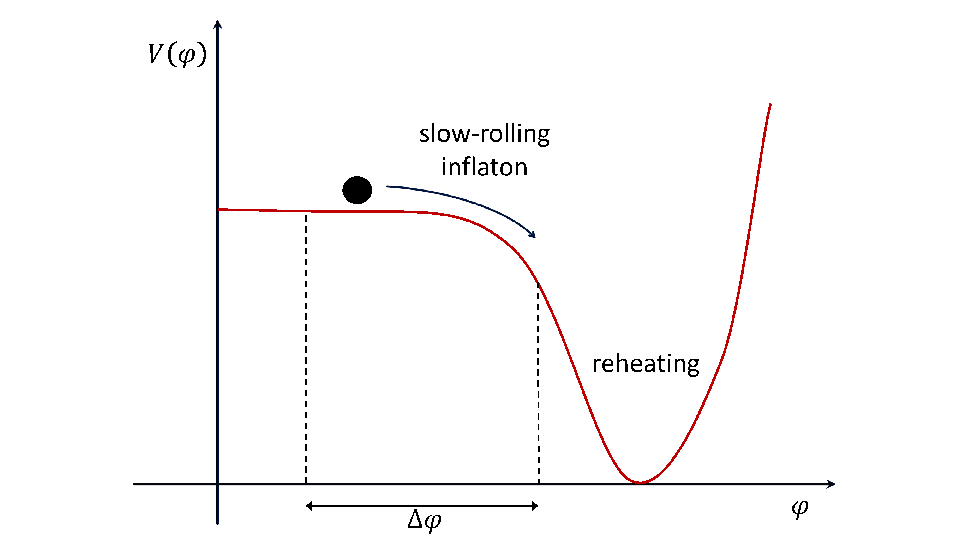
\includegraphics[width=0.65\linewidth, height=0.25\textheight]{Images/Chap1/GWFromInflation_Fig1}
	\caption{Example of inflationary potential with a flat region. After the slow-roll of the inflaton field $\phi$, the reheating phase starts. The field oscillates around the minimum of the potential and decays in other particles. $\Delta\phi$ indicates the inflaton excursion between the horizon exit of a comoving scale and the end of inflation \cite{GWFromInflation:Intro}. }
	\label{fig:gwfrominflationfig1}
\end{figure}

\subsection{Slow-roll parameters}

We quantify now under which circumstances a scalar field may give rise to a period of inflation.
Considering the background scalar field $ \phi $ (homogeneous and isotropic), the equation of motion (\ref{eomForPhi}) becomes
\begin{equation}
	\label{eomHomogeneousField}
	\ddot{\phi} + 3H \dot{\phi} + V'(\phi) = 0.
\end{equation}
If the \textit{slow-roll} condition $ \phi^{2} \ll V(\phi) $ is satisfied, the scalar field slowly rolls down its potential. Such a period can be achieved if the inflaton field is in a region where the potential is sufficiently flat. Since the potential is flat we may also expect that $\ddot{\phi}$ is negligible as well. We  assume that this is true and we quantify now this condition.

Requiring the slow-roll condition, the Friedmann equation (\ref{friedmannEquations1}) becomes 
\begin{equation}
	\label{friedMannEqDuringInflation}
	H^{2} \simeq \frac{8\pi G}{3} V(\phi),
\end{equation}
where we assumed that the inflaton field dominates the energy density of the universe. Moreover, assuming also $\ddot{\phi}$ negligible, we obtain the new equation of motion
\begin{equation}
	\label{newEQMphiDotDotNegligible}
	3H\dot{\phi} = -V'(\phi).
\end{equation}
Using (\ref{newEQMphiDotDotNegligible}) and the slow-roll condition (\ref{conditionFlatPotential}), we obtain
\begin{equation}
	\label{condition1}
	\frac{(V')^{2}}{V} \ll H^{2},
\end{equation}
and considering $\ddot{\phi} \ll 3H\dot{\phi}$,
\begin{equation}
	\label{condition2}
V'' \ll H^{2}.	
\end{equation}
These two conditions represent the flatness conditions of the potential, which are conveniently parametrized in terms of the so-called \textit{slow-roll parameters}.
The slow-roll parameters quantify the slow-roll regime dynamics in order to give predictions of specific models and to compare them with others and with observations.

Firstly, we define the $\epsilon$ parameter
\begin{equation}
	\label{epsilon}
	\epsilon = - \frac{\dot{H}}{H^{2}},
\end{equation}
which describes how much $ H $ changes during inflation.
To relate this variable to the slow-roll relation $ \dot{\phi}^{2} \ll V(\phi) $, let us derive the first Friedmann equation (neglecting the curvature),
\begin{equation}
	\label{derivingEpsilon1}
	H^{2}=\frac{8\pi G}{3}\rho_{\phi} = \frac{8\pi G}{3} \Big (\frac{1}{2}\dot{\phi}^{2} + V(\phi) \Big ),
\end{equation}
obtaining
\begin{equation}
	\label{FriedmannDerived}
	2H\dot{H} = \frac{8\pi G}{3} \Big (\dot{\phi} \ddot{\phi} + V'(\phi)\dot{\phi} \Big ).
\end{equation}
Now, inserting the equation of motion of the inflaton $ \ddot{\phi} = -3H\dot{\phi} - V'  $ in (\ref{FriedmannDerived}), we obtain
\begin{equation}
	\label{Hdot}
	\dot{H} = -4\pi G\dot{\phi}^{2}.
\end{equation}
Finally, using $ H^{2}=(8\pi G/3)V(\phi) $, 
\begin{equation}
	\label{epsilon2}
	\epsilon= - \frac{\dot{H}}{H^{2}}=4\pi G \frac{\dot{\phi}^{2}}{H^{2}} \simeq \frac{3}{2} \frac{\dot{\phi}^{2}}{V(\phi)},
\end{equation}
where the last equality si valid only in the slow-roll regime. Therefore, we can interpret $\epsilon$ as the ratio between the kinetic energy and the potential. 
Hence, assuming $ V(\phi) \gg \dot{\phi}^{2}  $, we obtain 
\begin{equation}
	\label{conditionEpsilon}
	\epsilon \ll 1 .
\end{equation}
Moreover, exploiting $ H\dot{\phi} \simeq -V' $, we can write
\begin{equation}
	\label{newEpsilon}
	\epsilon=4\pi G \frac{\dot{\phi}^{2}}{H^{2}} \simeq \frac{1}{16\pi G} \Big (\frac{V'}{V} \Big )^{2},	
\end{equation}
which means that if $\epsilon \ll 1 $ , $V'$ is small and the potential is flat. Thus, $\epsilon$ quantifies the flatness of the potential.

Considering the second slow-roll condition $ \ddot{\phi} \ll 3H\dot{\phi} $, we can define the second slow-roll parameter as 
\begin{equation}
	\label{etaParameter}
	\eta = - \frac{\ddot{\phi}}{H\dot{\phi}} \ll 1.
\end{equation}
As we have done for $\epsilon$ we can relate this expression to the potential. To do this we can derive $ \dot{\phi} \simeq -V'/3H $, obtaining
\begin{equation}
	\label{phiDerivedEtaParameter}
	\ddot{\phi} = -\frac{V'' \dot{\phi}}{3H} + \frac{\dot{H}}{3H^{2}}V'.
\end{equation}
Plugging this into the definition of $\eta$ we obtain
\begin{equation}
	\label{eta2}
	\eta \simeq \frac{V''}{3H^{2}} - \frac{\dot{H}}{H^{2}}\frac{V'}{3H\dot{\phi}} \simeq \eta_{V} - \epsilon,
\end{equation}
where $ \frac{V'}{3H\dot{\phi}} \simeq -1 $, and we have defined $ \eta_{V}=\frac{V''}{3H^{2}} $. Thus, again, having $\eta \ll 1$ means to have a flat potential.

A successful period of inflation requires that $ \epsilon, |\eta| \ll 1 $. Moreover, exists a hierarchy of slow-roll parameters: for example, one can define the slow-roll parameter related to the third derivative of the potential
\begin{equation}
	\label{secondOrderParameter}
	\xi^{2} = \Big (\frac{1}{4\pi G} \Big )^{2} \Big (\frac{V'V'''}{V^{2}}\Big ),
\end{equation}
which is a second order slow-roll parameter. The third derivative of the potential corresponds to an eventual self-interaction of the inflaton field. 
One can use these parameters with the data collected from observations to reconstruct the shape of the potential.
At first-order in the slow-roll parameters $\epsilon$ and $\eta$ can be considered constant, since the potential is very flat and their derivatives are higher orders in these parameters. In fact, it is easy to see that $ \dot{\epsilon},\dot{\eta} = \mathcal{O}(\epsilon^{2},\eta^{2}) $.

If we write $ \epsilon = - \dot{H}/H^{2} $, we can notice that
\begin{equation}
	\label{scaleFactorParameter}
	\ddot{a}=\dot{\dot{a}}=\dot{(aH)}=\dot{a}H + a\dot{H}=aH^{2}\Big (1+\frac{\dot{H}}{H^{2}}\Big ) = aH^{2}(1-\epsilon) .
\end{equation} 
Thus, inflation can be attained only if $\epsilon < 1$. As soon as this condition fails, inflation ends.

This condition alone can be sufficient to realise inflation. However, having also $\eta \ll 1 $  assure that inflation lasts for long enough. In fact, $ \eta = - \frac{\ddot{\phi}}{H\dot{\phi}}  \ll 1 $ both ensures that inflation is an attractor solution and that $\dot{\phi}$ remains constant and small for long enough. In other words, $\eta$ controls the duration of inflation.

Despite the semplicity of the inflationary theory, the number of inflationary models that have been proposed so far is enormous, differing for the kind of potential and for the underlying particle phyisics theory. In the second chapter we will discuss about the most important models, but we just  mention here that the main classification in connection with the observations is the one in which the single-field inflationary models are divided into three broad groups as \textquotedblleft small field", \textquotedblleft large field" (or chaotic) and \textquotedblleft hybrid" type, according to the region occupied in the ($\epsilon$ - $\eta$) space by a given inflationary potential.

\section{Inflation and Cosmological Perturbations}
The description of the universe as a perfectly homogeneous and isotropic FRW model is an idealitation. Actually, we are interested in deviations from homogeneity and isotropy that enable us to characterise different models.

So far we have considered only the dynamics of a homogenous scalar field driving inflation. But to investigate inflation models in more detail, and to test theoretical predictions against cosmological observations, we need to consider inhomogeneous perturbations. 

Besides the background inflationary dynamics we have the evolution of  quantum fluctuactions of the inflaton field $ \delta\phi(t,\textbf{x}) $. In the inflationary model there are primordial energy density perturbations, associated with these vacuum fluctuations, which survive after inflation and are the origin of all the structures in the universe.

Once the universe became matter dominated ($ z \simeq 3200 $), primeval density inhomogeneites ($ \delta \rho/\rho \simeq 10^{-5} $) were amplified by gravity and grew into the structures we see today. The existence of these inhomogeneities was in fact confirmed by the COBE discovery of CMB anisotropies.

In this section we summarise how the quantum fluctuations of a generic scalar field evolve during an inflationary stage. For more details see \cite{Liddle:intro},\cite{NonGauss:Intro},\cite{Dodelson:Chap1}.

\subsection{Quantum Fluctuations}
Consider for semplicity a scalar field $ \phi $ (the inflaton) with an effective potential $ V(\phi) $ in a pure de-Sitter stage, during which the Hubble rate $ H $ is constant. 
We first split the field $ \phi(\tau,\textbf{x}) $ in the homogeoneous classical part, $ \phi(\tau) $, and its fluctuations $ \delta\phi(\tau,\textbf{x}) $,
\begin{equation}
	\label{splitInflatonTau}
	\phi(\tau,\textbf{x})=\phi(\tau) + \delta \phi(\tau,\textbf{x})
\end{equation}
where $ \tau $ is the conformal time, related to the cosmic time $ t $ through $ d\tau=dt/a(t) $.

We consider the Fourier transform of the fluctuations
\begin{equation}
\label{fourierTransform}
\delta\phi(\tau,\textbf{x})=\frac{1}{(2\pi)^{3}}\int d^{3}k e^{i \textbf{k}\cdot\textbf{x}}\delta\phi(\tau,k).
\end{equation}
Redefining  the scalar field as 
\begin{equation}
\label{fieldRedefinition}
\widetilde{\delta \phi}	= a\delta\phi,
\end{equation}
 we can promote it to an operator, which can be decomposed as 
 \begin{equation}
 	\label{quantitation}
 	\widetilde{\delta \phi}(\tau,\textbf{x})=\int \frac{d^{3} \textbf{k}}{(2\pi)^{3/2}} \big[u_{k}(\tau)a_{\textbf{k}}e^{i \textbf{k}\cdot\textbf{x}} + u_{k}^{*}(\tau)a_{\textbf{k}}^{\dagger}e^{-i \textbf{k}\cdot\textbf{x}}\big],
 \end{equation}
 where we have introduced the creation and annihilation operators $ a_{\textbf{k}} $ and $ a^{\dagger}_{\textbf{k}} $.
 The creation and annihilation operators for $\tilde{\phi}$ satisfy the standard commutation relations
 \begin{equation}
 	\label{commutationRelations}
 \big[a_{\textbf{k}},a_{\textbf{k}'}] = 0 \qquad \big[a_{\textbf{k}},a_{\textbf{k}'}^{\dagger}] = \delta^{(3)}(\textbf{k}-\textbf{k}'),
 \end{equation}
and the modes $ u_{k}(\tau) $ are normalized, so that they satisfy the condition
\begin{equation}
	\label{normalitation}
	u^{\ast}_{k} u_{k}' - u_{k} u'^{\ast}_{k} = -i,
\end{equation}
where primes denote derivatives with respect to the conformal time $ \tau $. 

Expanding the equation of motion for the scalar field (\ref{eomForPhi}) in the fluctuations $\delta\phi(\tau,\textbf{x})$ in Fourier space, we obtain
\begin{equation}
	\label{eomFluctuations}
	u''_{k}(\tau) + \Big[k^{2} - \frac{a''}{a} + \frac{\partial^{2} V}{\partial\phi^{2}}a^{2}\Big] u_{k}(\tau) = 0,
\end{equation}
 where $ m^{2}_{\phi} = \partial^{2} V / \partial\phi^{2} $ is the effective mass of the scalar field. This equation describes an harmonic oscillator with a frequency changing in time, due to the expansion of the universe.
 
 The modes $ u_{k}(\tau) $ at very short distances must reproduce the form for the ordinary flat space-time quantum field theory. Thus, well within the horizon in the limit $ k/aH \rightarrow \infty $, the modes should approach plane waves of the form
 \begin{equation}
 	\label{planeWave}
 	u_{k}(\tau) \rightarrow \frac{1}{\sqrt{2k}}e^{-ik\tau}.
 \end{equation}

Let us consider a special case where the inflaton is massless in a pure de-Sitter universe ($m_{\phi} = 0, H=constant $). In this situation, the equation (\ref{eomFluctuations}) becomes
\begin{equation}
\label{eomMasslessDesitter}
u''_{k}(\tau) + \Big[k^{2} - \frac{a''}{a}\Big]u_{k}(\tau) = 0.
\end{equation}
Using $a d\tau=dt$ and $ a \propto e^{Ht}$ in a de-Sitter stage, we obtain 
\begin{equation}
	\label{horizon}
	\frac{a''}{a}= \frac{2}{\tau^{2}}=2a^{2}H^{2}=\frac{2}{r_{H}^{2}},
\end{equation}
where $ r_{H} $ is the comoving Hubble radius.

Therefore, we can study (\ref{eomMasslessDesitter}) in two different regimes: the \textit{sub-horizon} regime where $ \lambda_{phys} \ll H^{-1} $, $ k^{2} \gg a^{2}H^{2} \simeq a''/a $, and the \textit{super-horizon} regime where $ \lambda_{phys} \gg H^{-1} $, $ k^{2} \ll a^{2}H^{2} \simeq a''/a $.

In the sub-horizon case the equation of motion reduces to the wave equation
\begin{equation}
\label{waveEquationFluctuation}
u''_{k} + k^{2}u_{k}=0\  \rightarrow\  u_{k}(\tau)= \frac{1}{\sqrt{2k}}e^{-ik\tau} ,
\end{equation}
and the field reads
\begin{equation}
	\label{fieldSubHorizon}
	 \delta\phi_{k}=u_{k}/a=\frac{1}{a}\frac{1}{\sqrt{2k}}e^{-ik\tau},
\end{equation}
from which we can notice that it has a decreasing amplitude $ |\delta\phi| = 1/a\sqrt{2k} $, which depends on the inverse of $ a $.

In the super-horizon regime we obtain the equation
\begin{equation}
	\label{superHorizon}
	u''_{k} + \frac{a''}{a}u_{k}=0.
\end{equation}
This equation is solved by
\begin{equation}
	\label{solutionSuperHorizon}
	u_{k}(\tau) = B(k)a(\tau) + A(k)a^{-2}(\tau),
\end{equation}
where A, B are integration constants in $ \tau $ which depends on $ k $. In terms of the field we get
\begin{equation}
	\delta\phi_{k} = B(k) + A(k)a^{-3}(\tau) \simeq B(k) = constant,
\end{equation}
where we have neglected the decaying term which gets washed away by inflation.
\begin{figure}
	\centering
	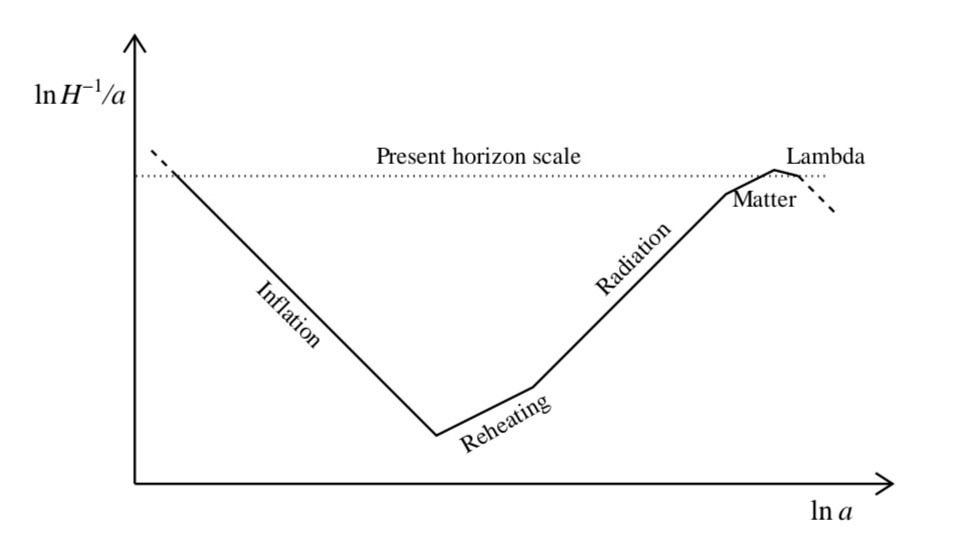
\includegraphics[width=0.85\linewidth, height=0.3\textheight]{Images/Chap1/ComovingScale}
	\caption{A plot of $\ln (H^{-1}/a)$ versus $\ln a$ shows the different
		epochs in the e-foldings calculation. The solid curve shows the
		evolution from the initial horizon crossing to the present, with
		the dashed lines showing likely extrapolations into the past
		and future. The condition for inflation is that  $ \ln  (H^{-1}/a) $ be
		decreasing. During reheating and matter
		domination $ H^{-1}/a \propto a^{1/2} $
		, while during radiation domination  $ H^{-1}/a \propto a $. The recent domination by dark energy has
		initiated a new era of inflation. The horizontal dotted line
		indicates the present horizon scale. The number of e-foldings
		of inflation is the horizontal distance between the time when
		$H^{-1}/a$ first crosses that value and the end of inflation \cite{Chap1:ComovingRadiusPlot}.} 
	\label{fig:comovingscale}
\end{figure}

We can fix the amplitude of the growing mode, $ B(k) $, by matching the (absolute value of) this solution to the plane wave solution (\ref{fieldSubHorizon}) when the fluctuation with wavenumber k leaves the horizon ($ k = aH $). This gives
\begin{equation}
	|B(k)|= \frac{1}{a\sqrt{2k}} = \frac{H}{\sqrt{2k^{3}}}.
\end{equation}
Therefore, the quantum fluctuations of the original scalar field $ \phi $ on super-horizon scales are constant,
\begin{equation}
	\label{frozenField}
	|\delta \phi_{k}| = \frac{|u_{k}|}{a} = \frac{H}{\sqrt{2k^{3}}}.
\end{equation}

From this simple computation we can see that inflation is able to provide a mechanism to generate density perturbations (and gravitational waves). To understand what is going on, a key ingredient is the decreasing with time of the comoving Hubble horizon $ (aH)^{-1} $ during inflation. The wavelength of a quantum fluctuation in the inflaton field soon exceeds the Hubble radius. The quantum fluctuations arise on scales which are much smaller than the comoving Hubble radius, that is the scale beyond which causal processes cannot operate. On small scales we can use the usual flat space quantum field theory to describe the scalar field vacuum fluctuations.
However, the inflationary expansion \textit{stretches} the wavelength of these fluctuations  outside the horizon. The quantum fluctuations of the inflaton are amplified (and frozen) on super-horizon scales, resulting in a net number of scalar field particles.

On large scales the perturbations just follow a classical evolution. Since microscopic physics does not affect the evolution of fluctuations when their wavelengths are outside the horizon, the amplitude of these inhomogeneites are "frozen" and fixed at some nonzero value $ \delta\phi $ at the horizon crossing.
The amplitude of the fluctuations on super-horizon scales then remains almost unchanged for a very long time, whereas the wavelength grows exponentially. Thus, these frozen fluctuations of the inflaton are equivalent to the appearance of a classical field $ \delta\phi $ that does not vanish after having averaged over some macroscopic interval of time. Moreover, the same mechanism also generates a stochastic background of gravitational waves.

The quantum fluctuations of the inflaton generate also fluctuations in the space-time metric, giving rise to perturbations of the curvature $ \mathcal{R} $. On super-horizon scales curvature fluctuations are frozen in and considered as classical.
When the wavelength of these perturbations re-enters the horizon, in the radiation or matter dominated epoch, the curvature perturbations of the space-time give rise to matter (and temperature) perturbations $ \delta \rho $ via the Poisson equation.
These fluctuations will then start growing, giving rise to the structure we observe today (Fig. \ref{fig:comovingscale} from \cite{Chap1:ComovingRadiusPlot}).



\subsection{Power spectrum}

To characterise the properties  of a perturbation field we introduce the \textit{power spectrum}.
Consider a random field $ f(t,\textbf{x}) $ that can be expanded in Fourier space as 
\begin{equation}
\label{fourierTransform}
	f(t,\textbf{x}) = \int \frac{d^{3}\textbf{k}}{(2\pi)^{3/2}} e^{i\textbf{k}\cdot \textbf{x}} f_{\textbf{k}}(t).
\end{equation}
The power spectrum $ P_{f}(k) $ can be defined by means the relation
\begin{equation}
\label{powerSpectrum}
\big<f_{\textbf{k}_{1}}f^{*}_{\textbf{k}_{2}}\big> \equiv \frac{2\pi^{2}}{k^{3}}P_{f}(k) \delta^{(3)}(\textbf{k}_{1}-\textbf{k}_{2}),
\end{equation}
where the angled brackets denote the ensemble average. The power spectrum measures the amplitude of the fluctuations at a given scale $k$. Indeed, if we consider the last definition, the mean square value of $f(t,\textbf{x})$ in real space is
\begin{equation}
\label{meanSquare}	
\big<f^{2}(t,\textbf{x})\big>= \int \frac{dk}{k} P_{f}(k).
\end{equation}
To describe the slope of the power spectrum  we define the $ \textit{spectral index}$   $n_{f}(k)$,
\begin{equation}
\label{spectralIndex}
n_{f}(k) - 1 \equiv \frac{d  \ln P_{f}}{d  \ln k}.
\end{equation}  
For the inflaton field quantum fluctuations $ |\delta \phi_{k}| = \frac{|u_{k}|}{a} $,
\begin{equation}
	\label{fluctuations}
	\big < \delta\phi_{\textbf{k}_{1}} \delta \phi^{*}_{\textbf{k}_{2}}\big>=\frac{2\pi^{2}}{k^{3}}|\delta \phi_{\textbf{k}_{1}}|^{2} \delta^{(3)}(\textbf{k}_{1}-\textbf{k}_{2}).
\end{equation}
Therefore,
\begin{equation}
\label{spectrumFluctuation}
P_{\delta \phi}(k) = \frac{k^{3}}{2\pi^{2}}|\delta \phi_{k}|^{2},		
\end{equation}
with $ \delta \phi_{k} \equiv u_{k}/a $.	

\subsection{Exact solution}
Now we briefly recap how to solve exactly the equation of motion for the modes $ u_{k} $ (\ref{eomFluctuations}). This equation can be rewritten in the form of \textit{Bessel equation},
\begin{equation}
	\label{bessel}
	u''_{k}(\tau) + \Big[k^{2} - \frac{\nu^{2}-1/4}{\tau^{2}}\Big] u_{k}(\tau)=0.
\end{equation}
In this form it is equivalent to the Bessel equation
\begin{equation}
	z^{2}y''(z) + zy'(z) + (z^{2}-\nu^{2})y(z)=0,
\end{equation}				
whose solutions are known to be of the form 
\begin{equation}
	\label{solutionPerturbations}
	u_{k}(\tau) = \sqrt{-\tau}\big [c_{1}(k)H^{(1)}_{\nu}(-k\tau) + c_{2}(k)H_{\nu}^{(2)}(-k\tau)],
\end{equation}
where $ H^{(1)}_{\nu} $ and $ H^{(2)}_{\nu} $ are the Henkel functions of first and second kind, respectively.
The parameter $ \nu $ can be expressed in terms of the slow roll parameters.
In the case of a quasi de-Sitter universe and  (little) massive scalar field we have the relation $ 3/2 - \nu \simeq \eta_{V} - \epsilon$.
 The requirement  of a light mass is due to the fact that if $ m^{2}_{\phi} \ge H^{2}$,  $ \delta \phi_{k} $ remains in the vacuum state and fluctuations get suppressed. From now we omit the subscript \textquotedblleft $V$" in $\eta$.
 
If we impose  that in the ultraviolet regime $ k \gg aH $ $ (-k\tau \gg 1) $, the solution matches the plane-wave solution $ e^{-ik\tau}/\sqrt{2k} $ that we expect in flat space-time. Knowing the asymptotic beheaviour of the Hankel functions on sub-horizon scales we obtain
\begin{equation}
\label{Hankel1}
H^{(1)}_{\nu}(x \gg 1) \sim \sqrt{\frac{2}{\pi x}} e^{i(x-\frac{\pi}{2}\nu-\frac{\pi}{4})} 
\quad
H^{(2)}_{\nu}(x \gg 1) \sim \sqrt{\frac{2}{\pi x}} e^{-i(x-\frac{\pi}{2}\nu-\frac{\pi}{4})},
\end{equation}
and on super-horizon scales we have
\begin{equation}
\label{Hankel2}
H^{((1)}_{\nu}(x \ll 1) \sim \sqrt{\frac{2}{\pi}}e^{-i\frac{\pi}{2}}2^{\nu-\frac{3}{2}}\frac{\Gamma(\nu)}{\Gamma(3/2)}x^{-\nu}.	
\end{equation}
We can set in (\ref{solutionPerturbations})  $ c_{2}(k)=0 $ and $ c_{1}(k)=\frac{\sqrt{\pi}}{2}e^{i(\nu + \frac{1}{2})\frac{\pi}{2}} $.

We finally obtain for the fluctuations $ |\delta \phi_{k}| $ 
\begin{equation}
	\label{solutionDeltaPhi}
	|\delta \phi_{k}|= \frac{H}{\sqrt{2 k^{3}}}\Big (\frac{k}{aH}\Big)^{\frac{3}{2}-\nu},
\end{equation}
yielding for the power spectrum (\ref{spectrumFluctuation})
\begin{equation}
	\label{PowerSpectrumperturbation}
	P_{\delta \phi}(k) = \Big (\frac{H}{2\pi}\Big)^{2}\Big (\frac{k}{aH}\Big)^{3-2\nu},
\end{equation}
where $ \nu $ is given by $ 3/2 - \nu \simeq \eta_{V} - \epsilon$.

In the power spectrum just computed there is an inconsistency. In the computation the scalar field is perturbed on a unperturbed spacetime. Thus, we should also include perturbations of the metric to have a correct result. To do so, we need to consider scalar perturbations of the metric and use gauge invariant quantities. But before doing that, we are going to consider the tensorial perturbations of the metric: the gravitational waves.

\subsection{Gravitational waves}
Inflation predicts the existence of a scale invariant spectrum of primordial gravitational waves, sourced by the same quantum fluctuations described in the previous sections. Gravitational waves are only weakly coupled to matter fields, and move freely through the universe from the moment they are produced.

The perturbations of the inflaton field will induce perturbations of the metric. This leads to a stochastic background of gravitational waves (GW),  which are represented by tensor perturbations of the metric.
A stochastic background of waves is a continuos set of waves, fully characterized  only by their global statistic properties. It consists of a signal coming from every direction in the sky. It is different from the signals coming from astrophysical sources (merging neutron stars,  binary black holes...), which come from a specific direction in the sky. 
In this section we explain how inflation can generate this stochastic background. 

We start considering the perturbed spatially flat FLRW metric, where we neglect scalar and vector perturbations,
\begin{equation}
	ds^{2} = -dt^{2} + a^{2}(t)[\delta_{ij} + h_{ij}]dx_{i}dx_{j},
\end{equation}
with $ h_{ij} $, in the so called Transvere-Traceless gauge (TT gauge), are such that
\begin{equation}
	h_{ij}=h_{ji} \qquad h^{i}_{i}=0 \qquad h^{i}_{j|i} = 0.
\end{equation}
 At linear level Einstein's equations for $ h_{ij} $ are 
 \begin{equation}
 	\ddot{h}_{ij} + 3H\dot{h}_{ij} - \frac{\nabla^{2}h_{ij}}{a^{2}}= \Pi^{TT}_{ij},
 \end{equation}
where $\Pi^{TT}_{ij}$ is a tensor, with the same properties of $ h_{ij} $, which is a source term coming from possible anisotropic stress of the matter source. It is related  to the last term of the stress-energy tensor of a perfect fluid $ T_{\mu\nu} = (\rho + P)u_{\mu}u_{\nu} + Pg_{\mu\nu} + \Pi_{\mu\nu}$, called anisotropic stress tensor, which can get a contribution in the case of astrophysical sources when we have a non vanishing quadrupole moment. We will see that this term is also important to describe the gravitational waves emitted in the reheating phase.
However, at first order, it is vanishing during single field inflation and the equation of $ h_{ij} $ becomes 
\begin{equation}
	\label{eqh}
		\ddot{h}_{ij} + 3H\dot{h}_{ij} - \frac{\nabla^{2}h_{ij}}{a^{2}}=0,
\end{equation}
which is similar to the equation for the quantum vacuum fluctuation in the case of a massless scalar field.
Since there is no source term, GW are the intrinsic quantum fluctuations of the metric. Moreover, they provide a \textit{smoking gun} of inflation and would be the first ever detected evidence of quantum gravity.

The equation (\ref{eqh}) describes the evolution of the tensor $ h_{ij} $, which has 2 independent DOF, corresponding to the two possible polarizations of GW $ \lambda = (+,\times) $. Such object can be decomposed in Fourier space as 
\begin{equation}
	\label{fouriewrh}
	h_{ij}(\tau,\textbf{x}) = \sum_{+\times} \int \frac{d^{3} k}{(2\pi)^{3}}e^{i\textbf{k}\cdot \textbf{x}}h_{\lambda}(\textbf{k},\tau)\epsilon^{\lambda}_{ij}(\textbf{k}),
\end{equation}
where $ \epsilon^{\lambda}_{ij}(\textbf{k}) $ are the polarization tensors, which satisfy
\begin{equation}
	\epsilon_{ij}=\epsilon_{ji} \qquad \epsilon^{i}_{i}=0 \qquad  k^{i}\epsilon_{ij}(\textbf{k}) =0,
\end{equation}
 with normalitation conditions
 \begin{equation}
 \epsilon_{ij}^{\lambda}(\textbf{k})\epsilon^{*ij}_{\lambda'}(\textbf{k})=\delta_{\lambda\lambda'}
 \qquad
 \big (\epsilon_{ij}^{\lambda}(\textbf{k})\big)^{*} = \epsilon_{ij}^{\lambda}(-\textbf{k}).
 \end{equation}
Considering a plane monochromatic gravitational wave propagating in the $\hat{z}$ direction in Fourier space we have
\begin{equation}
	\epsilon^{+}_{ij} = 
	\begin{pmatrix}
		1 & 0 \\
		0 & -1
	\end{pmatrix}
\qquad
\epsilon^{\times}_{ij} = 
\begin{pmatrix}
	0 & 1 \\
	1 & 0
\end{pmatrix}
\end{equation}
\begin{equation}
	h_{ij}(\textbf{k},\tau) = h_{+}(\textbf{k},\tau)\epsilon_{ij}^{+}(\textbf{k}) + 
	h_{\times}(\textbf{k},\tau)\epsilon_{ij}^{\times}(\textbf{k}),
\end{equation}
and the tensor $ h_{ij} $ satisfies
\begin{equation}
	\ddot{h}_{\lambda} + 3H\dot{h}_{\lambda}+ k^{2}\frac{h_{\lambda}}{a^{2}}=0,
\end{equation}
which is the same for each polarization state.

On super-horizon scales, $ k\ll aH $, the solution for $ h_{+,\times} $ is given by a constant plus a decaying mode. Using the canonical normalitation
\begin{equation}
|h_{+,\times}|= \sqrt{32\pi G}|\phi_{+,\times}| = \sqrt{32\pi G} \frac{H}{\sqrt{2k^{3}}}\Big (\frac{k}{aH}\Big)^{-\epsilon}.
\end{equation}
On sub horizon scales ($ k \gg aH $) we have $ h_{+,\times}=\frac{e^{-ik\tau}}{a(\tau)} $.

For the power spectrum we obtain
\begin{equation}
\label{spectumGW}
P_{T}(k)=\frac{k^{3}}{2\pi^{2}}\langle h^{*}_{ij}h^{ij}\rangle=\frac{16}{M_{pl}^{2}}\Big(\frac{H}{2\pi}\Big )^{2}\Big (\frac{k}{aH}\Big)^{-2\epsilon},
\end{equation}   
where $ H $ indicates the Hubble rate during inflation and we have summed the two polarizations $ (+,\times) $.

Therefore we can define the spectral index of inflationary gravitational waves as
\begin{equation}
n_{T} = \frac{d \ln P_{T}}{d \ln k} = -2\epsilon.
\end{equation}
In the simplest models one has $ \epsilon > 0 $, so $ n_{T} $ is always red-tilted (on smaller scales the amplitude decreases).
Since during inflation $P_{T} $ $\sim$ $ H^{2} $ and $ H^{2} \simeq \frac{V}{M^{2}_{pl}} $, detecting the tensor spectrum would give us the energy scale of inflation ($ E_{inf} \simeq V^{1/4} $, see later). 

\subsection{Primordial curvature perturbation}
In the standard slow-roll inflationary models the fluctuations of the inflaton field are responsible for the curvature perturbations.
 As said, they are (nearly) frozen on super-horizon scales. When they re-enters the horizon lead to pertubations of matter that give rise the structure we see today.
 
To characterise the scalar and curvature perturbations we need gauge invariant quantities.
A complete treatment of this argument is in \cite{NonGauss:Intro}. Here we just summarise the main points.

Consider the perturbed FRW metric at first order including only scalar perturbations and expressed with the conformal time $ \tau=\int dt/a(t) $
\begin{equation}
\label{metricPerturbed}
ds^{2}=a^{2}(\tau) \big [-(1+2\Psi)d\tau^{2} + (1-2\Phi)\delta_{ij}dx_{i}dx_{j} \big].
\end{equation}
The first gauge invariant quantity we consider is
\begin{equation}
	\label{zeta}
	-\zeta \equiv \hat{\Phi} + \mathcal{H}\frac{\delta \rho}{\rho'},
\end{equation}
where $\mathcal{H} \equiv a'/a$ is the Hubble parameter in conformal time and the prime denote differentiation w.r.t it. $\hat{\Phi}$ is referred to as the \textit{curvature perturbation}. This quantity, however, is not gauge invariant since it changes under a transformation on costant time hyper-surfaces $\tau$ $\rightarrow$ $ \tau + \alpha $. Instead, combining the $\hat{\Phi}$ transformation and the gauge transformation for scalars comes out that $\zeta$ in (\ref{zeta}) is gauge invariant. This quantity is called \textit{gauge-invariant curvature perturbation of the uniform energy-density hypersurfaces}.

To obtain the $\zeta$ power spectrum consider another gauge invariant quantity called \textit{curvature perturbation on comoving hyper-surfaces}. In the case of a stress-energy tensor of a single scalar field it reads
\begin{equation}
	\label{R}
	\mathcal{R} \equiv \hat{\Phi} + \frac{\mathcal{H}}{\phi'}\delta \phi.
\end{equation}
The comoving curvature perturbation $\mathcal{R}$ is related to the curvature perturbation $\zeta$ by
\begin{equation}
	- \zeta = \mathcal{R} + \frac{2\rho}{9(\rho + P)} \Big (\frac{k}{aH}\Big)^{2}\Psi,
\end{equation}
where $\Psi$ is the perturbation that appears in the metric. 
From this relation we obtain that on large scales $\mathcal{R} \simeq -\zeta$.

In the previous sections we obtained the power spectrum of  the primordial fluctuations of the inflaton (\ref{PowerSpectrumperturbation}). However, we computed it without taking into account the perturbation of the metric.
To do so, we define a new gauge-invariant quantity called  \textit{Sasaki-Mukhanov variable},
\begin{equation}
	\label{sasaki-mukhanov}
	\mathcal{Q}_{\phi} \equiv \delta \phi + \frac{\phi'}{\mathcal{H}}\Phi.
\end{equation}
Introducing the field $\tilde{\mathcal{Q}}_{\phi}=aQ_{\phi}$ the Klein-Gordon equation reads \cite{NonGauss:Intro}
\begin{equation}
	\label{finalEOM}
\tilde{\mathcal{Q}}'' + \Big (k^{2} - \frac{a''}{a} + \mathcal{M}_{\phi}^{2}a^{2}\Big)\tilde{\mathcal{Q}}_{\phi} = 0,
\end{equation} 
where 
\begin{equation}
 \mathcal{M}^{2}_{\phi}=\frac{\partial^{2} V}{\partial \phi^{2}} - \frac{8\pi G}{a^{3}}\Big (\frac{a^{3}}{H}\dot{\phi}^{2}\Big)
\end{equation}
is an effective mass of the inflaton field. At lowest orders in the slow-roll parameters the latter expression reduces to $ \mathcal{M}^{2}_{\phi}/H^{2} = 3\eta-6\epsilon $. Solving (\ref{finalEOM}) by means of the Hankel functions, as we did in the previous sections, we obtain at super-horizon scales and at  lowest order in the slow-roll parameters the complete solution
\begin{equation}
	\label{solutionPerturbation}
	|Q_{\phi}(k)| = \frac{H}{\sqrt{2k^{3}}}\Big (\frac{k}{aH}\Big)^{3/2-\nu},
\end{equation}
where $ \nu \simeq 3/2 + 3\epsilon - \eta $.
This solution leads to a power spectrum
\begin{equation}
\label{PSQ}
P_{\mathcal{Q}}=\Big (\frac{H}{2\pi} \Big)^{2}\Big(\frac{k}{aH}\Big)^{3-2\nu}.
\end{equation}
Now, returning to the gauge-invariant curvature perturbation $ \mathcal{R} $ (\ref{R}), we can easily express it in function of the Sasaki-Mukhanov variable. Using (\ref{sasaki-mukhanov}) results
\begin{equation}
	\label{expressionR}
	\mathcal{R}=\dfrac{\mathcal{H}Q_{\phi}}{\phi'} = \frac{H Q_{\phi}}{\dot{\phi}},
\end{equation}
where we have expressed $ \mathcal{R} $ in terms of the cosmic time.
Finally, using (\ref{PSQ}), we obtain the power spectrum of the curvature perturbation $\mathcal{R}$,
\begin{equation}
\label{PR}
P_{\mathcal{R}}=\Big (\frac{H}{\dot{\phi}}\Big)^{2}P_{\mathcal{Q}}= \Big (\frac{H^{2}}{2\pi \dot{\phi}}\Big)^{2}\Big(\frac{k}{aH}\Big)^{3-2\nu} \simeq \Big(\frac{H^{2}}{2\pi\dot{\phi}}\Big)^{2}_{*},
\end{equation}
where  the asterisk denotes quantities evaluated at the epoch a given perturbation mode leaves the horizon during inflation, that is $ k=aH $.
The last equation shows that the curvature perturbations remains  time-independent on super-horizon scales. In the \textit{uniform curvature gauge}, where $ \Phi=0 $, we have $ \zeta \simeq - \mathcal{H}\delta \rho/\rho' $. So, we can connect the inflaton perturbations to observable quantities.
The solution obtained for $\zeta$ is valid  throughout the different evolution eras of the universe until the mode remains super horizon.

From (\ref{PR}) we can easily obtain the spectral index of the curvature perturbation (at lowest order in the slow-roll approximation)
\begin{equation}
\label{spectralIndex}
n_{\mathcal{R}}-1\equiv \frac{d \ln P_{\mathcal{R}}}{d \ln k} = 3 - 2\nu=-6\epsilon + 2\eta.
\end{equation}
Inflationary models predict a power spectrum of density perturbations very close to 1. The specific case in which $ n_{s}=1 $ is called \textit{Harrison-Zel'dovich} spectrum, and means that the amplitude of the inflaton pertubations does not depend on the cosmological scale.

The curvature mode is the quantity which allows to connect the primordial perturbations produced during inflation to the observables.
This result comes from the fact that in single-field slow roll models the intrinsic entropy perturbation of the inflaton field is negligible on large scales. This result holds also during the reheating phase after inflation\cite{NonGauss:Intro}. 

\subsection{Consistency relation}
In the single-field models an important consistency relation holds. To derive it, we introduce the \textit{tensor-to-scalar ratio}
\begin{equation}
\label{tensorScalarRatio}
r(k_{*})\equiv \frac{P_{T}(k_{*})}{P_{S}(k_{*})},
\end{equation}
that yields  the amplitude of the GW with respect to that of the scalar perturbations at some pivot scale $ k_{*} $.

We can rewrite the power spectrum $ P_{\mathcal{R}} $ in (\ref{PR}) as function of the slow-roll parameters using the fact that $ \epsilon=-\dot{H}/H^{2}=4\pi G\dot{\phi^{2}}/H^{2} $, obtaining
\begin{equation}
	\label{PSRelatedToEpsilon}
P_{\mathcal{R}}(k)=\frac{1}{2M_{P}^{2}\epsilon}\Big (\frac{H}{2\pi}\Big)^{2}\Big (\frac{k}{aH}\Big)^{n_{\mathcal{R}}-1}	,
\end{equation}
that yields $ r=16\epsilon $.

Furthermore, we have shown that a nearly scale-invariant spectrum of tensor modes is expected, being $ n_{T}=-2\epsilon $. Therefore, at the lowest order in the slow-roll parameters, one finds the consistency relation
\begin{equation}
	\label{consistencyRelation}
	r=-8n_{T}.
\end{equation}
This equality can be proved only with a measure of the tensor power spectrum (not only the amplitude, but also  its spectral index i.e. its shape).

Since a large spectral index would invalidate the consistency relation, it will be very hard to measure any scale dependance of the tensors assuming the consistency relation valid.
The current best bound on $ \textit{r} $ comes from the joint analysis of \textit{Planck} and BICEP/Keck 2018, which yields $ r < 0.032 $ at $ 95 \% $ C.L. for $ k_{*}$ = $ 0.05\ Mpc^{-1} $ \cite{Intro:ConstraintsOnr}. 

Finally, we can connect the energy scale of inflation to the tensor-to-scalar ration $ r $.
From $ H^{2}=8\pi GV/3 = V/3M_{pl}^{2}$ we can link the energy scale of inflation, at the time when the pivot scale leaves the horizon, directly to the parameter $\epsilon$ using (\ref{PSRelatedToEpsilon}),
\begin{equation}
	V=24\pi^{2}M_{pl}^{4}P_{\mathcal{R}}\epsilon =(3\pi^{2}P_{\mathcal{R}}/2)M_{pl}^{4}r.
\end{equation}
Thus, considering  the scalar amplitude estimated  by the Planck Collaboration \cite{Plank2015:Chap1}, one gets  the following relation between the energy scale of inflation at the time when the pivot scale leaves the Hubble radius, and the tensor-to-scalar ratio:
\begin{equation}
	\label{energyScaleInflation-r}
	V=(1.88\times10^{16}GeV)^{4}\frac{r}{0.10}.
\end{equation}
Then we have a direct link between $ r $ and the energy scale of inflation.

In the next chapter we will overview the most important models of inflation and we will introduce the important stage of reheating by means of a toy model.
The reheating phase is the main focus of this work since it leads to very interesting effects and physics. Moreover, the gravitational waves generated by reheating are very different from those generated by inflation and could be detected by future experiments providing an observational window of such period.

\chapter{Inflation Zoology and Reheating}
So far we have not discussed the form of the inflaton potential, $ V(\phi) $. A simple model of inflation was proposed by Guth in 1981 to solve the horizon and flatness problems discussed in the first chapter \cite{Guth:Intro}.
In this model, called  \textit{Old Inflation} scenario, the inflaton is initially trapped in a metastable false vacuum during inflation. Subsequently  it moves towards the true vacuum via a first-order transition. In this scenario inflation is then an exponential expansion of the universe in the supercooled false vacuum state that makes the universe very big and very flat. However, as pointed out by Guth in the paper, this type of inflation produces a random nucleation of bubbles that lead a highly inhomogeneous universe.

This problem is solved by the \textit{New Inflation} in 1981-1982 \cite{Chap2: Linde_NewInflation} . In this model, inflation may begin either in the false vacuum, or in an unstable state at the top of the effective potential. Then the inflaton field slowly rolls down to the minimun of the  potential. However, the useful part of inflation responsible for the homogeneity of the universe does not occur in the false vacuum state in this model. Unfortunately, also this picture has problems. It works only if the effective potential of the field $ \phi $ has a very flat plateau near $\phi=0$, which is somewhat artificial. Moreover, in most versions of this scenario the inflaton field  has an extremelly small coupling constant, so it could not be in thermal equilibrium  with other matter fields.

However, in the beginning of the 80's, on the basis of all available observations (CMB, abundance of light elements) everybody believed that the universe was in a state of thermal equilibrium from the very beginning and the stage of inflation was just an intermediate stage of the evolution of the universe.

In the 1983 the \textit{Chaotic Inflation} resolved all problems of old and new inflation \cite{ChaoticInflationLinde:Chap2}. According to this scenario, inflation may begin even if there was no thermal equilibrium in the early universe and it may occur in the scenarios with simplest quadratic potential. Moreover, it is not limited to theories with polynomial potentials: chaotic inflation occurs in any theory where the potential has a sufficiently flat region, which allows the existence of the slow-roll regime, as described in the previous chapter. A review of the hystory of inflation can be found in \cite{Chap2:Linde_HystoryInflation}.  

The different kinds of single-field inflationary models can be classified in the following way. The first class consists of the \textit{large field} models, in which the initial value of the inflaton is large and it slowly rolls down towards  the potential minimum at smaller $\phi$. Chaotic inflation is one of the representative models of this class. The second class consists of the \textit{small fied} models, in which the inflaton field is small initially and slowly evolves toward the potential minimum at larger $\phi$. An example of this type is new inflation. The third class consists of the \textit{hybrid inflation} models, in which inflation typically ends by a phase transition triggered by the presence of a second scalar field.
Several models of inflation can involve a coupling with gauge fields or other scalar fields. These models are very interesting because they can give rise to a source of gravitational waves and curvature perturbations \cite{GWFromInflation:Intro}. 

The main reheating models discussed in the literature are concentrated on the end of inflation in the chaotic and hybrid scenarios. Thus, in the first part of this chapter we review these important models. Beside that, we discuss also the Guth and natural inflation models (the second is an example of small-field model). In the second part,  we start to focus on the main topic of this work: the reheating phase. We'll start considering an elementary, simple scenario of reheating. From chapter 4 we will see that, instead, reheating models have very complicate and non-linear dynamics. 

\section{Inflationary Models}
\subsection{Guth's Inflation}
We start from the Guth model of inflation because it contains very interesting points such as entropy production and the random nucleation of bubbles, phenomena that also occurs in the non-linear stages of reheating \cite{Guth:Intro}.
This model was introduced to solve the horizon and flatness problem: initially, indeed, the early universe was assumed to be highly homogeneous, despite to the fact that separated regions were causally disconnected, and the initial value of the Hubble constant had to be extremelly fine-tuned to produce the flat universe we see today.

In this scenario the universe is assumed to be homogeneous and isotropic, and then is described by the Robertson-Walker metric that we rewrite:
\begin{equation}
	\label{metricCh2}	
	ds^{2}   = - dt^{2} + a^{2}(t)\Big[\frac{dr^{2}}{1-kr^{2}}  +  r^{2}(d\theta^{2} + sin^{2} \theta d\phi^{2})\Big], 
\end{equation}
where $ k=+1,-1,0 $ denotes a closed, open, or flat universe; $ a(t) $ is the scale factor.
As seen, the evolution of the scale factor is governed by the Friedmann equations
\begin{equation}
	\label{friedmannEquations1Chap2}
	H^{2}=\frac{8\pi G}{3}\rho - \frac{k}{a^{2}},
\end{equation}
\begin{equation}
	\label{friedmannEquations2Chap2}	
	\frac{\ddot{a}}{a} = -\frac{4\pi G}{3}(\rho + 3P),
\end{equation}
where $ H  $ is the Hubble constant. We rewrite the conservation of energy as
\begin{equation}
\label{Chap2:ConservationEnergy}
\frac{d}{dt}(\rho a^{3})=-p\frac{d}{dt}(a^{3}).
\end{equation}
In the standard Big-Bang model one also assumes that the expansion is adiabatic,
\begin{equation}
\label{Chap2:entropy1}
\frac{d}{dt}(sa^{3})=0,
\end{equation}
where $ s $ is the entropy density.

To study the evolution of the universe we need an equation of state for matter. At high temperatures, however, is a good approximation to consider an ideal quantum gas of massless particles. Let $ g_{*}(T) $ the effective number of degrees of freedom, the thermodynamics functions are given by
\begin{equation}
\label{Chap2EnergyDensity}
\rho=\frac{\pi^{2}}{30}	g_{*}(T)T^{4,}	
\end{equation}
\begin{equation}
\label{s}
s=\frac{2\pi^{2}}{45}g_{*}(T)T^{3}
\end{equation}
\begin{equation}
	\label{n}
	n=\frac{\zeta(3)}{\pi^{2}}g'(T)T^{3},
\end{equation}
where $ n $ denotes the particle number density and $\zeta(3)=1.202...$ is the Riemann zeta function.
We can rexpress the second Friedmann equation (\ref{friedmannEquations1Chap2}) solely in terms of the temperature. To do so, we substitute (\ref{Chap2EnergyDensity}) in (\ref{friedmannEquations1Chap2})  obtaining
\begin{equation}
	\label{Chap2:H-Temperature}
	H^{2}=\frac{4\pi^{3}G}{45}g_{*}T^{4},
\end{equation}
where we have neglected  the curvature term $ K/a^{2} $.
The conservation of entropy equation (\ref{Chap2:entropy1}) yields
\begin{equation}
	\label{Chap2entropy2}
	\dot{s} + 3Hs=0.
\end{equation}
Using  (\ref{s}) in this equation we obtain a direct relation between the Hubble constant and the temperature 
\begin{equation}
	\label{Chap2:relationTemperatureEntropy}
	H=-\frac{\dot{T}}{T},
\end{equation}
which, substituted in (\ref{Chap2:H-Temperature}), yields the Friedmann equation (\ref{friedmannEquations1Chap2}) expressed only in terms of the temperature T: 
\begin{equation}
	\label{Chap2:Friedmann-Temperature}
	\Big(\frac{\dot{T}}{T}\Big)^{2}=\frac{4\pi^{3}}{45}Gg_{*}(T)T^{4}.
\end{equation}

Guth in his paper stated that to solve the horizon and flatness problems it is crucial the violation of the adiabaticity condition by means a huge entropy production during the inflationary stage.
Suppose that the equation of state for matter exhibits a first-order phase transition at some critical temperature $ T_{c} $ (of the order of the GUT scale $T_{GUT}\simeq 10^{14}-10^{15}$ Gev). For example, we can have a phase-transition which causes a SSB of a group of a GUT theory. At higher temperature than $ T_{c} $ the inflaton is in thermal equilibrium with other particles.
As the universe expands, the system is not cooling toward the true vacuum, but rather towards some metastable false vacuum with an energy density $ \rho_{0} $ which is necessarily higher than that of the true vacuum. The inflaton is trapped in this state (Fig. \ref{fig:guthinflationfig5} from \cite{Chap2:Fig1}).
\begin{figure}
	\centering
	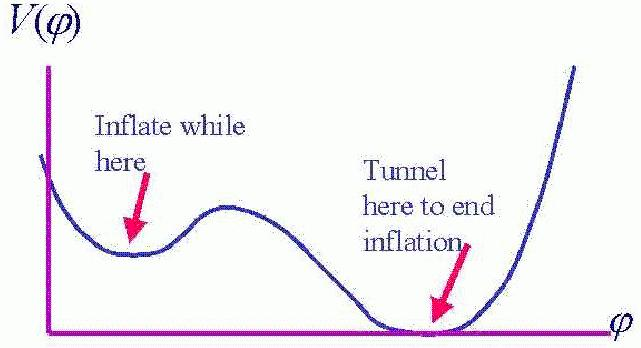
\includegraphics[width=0.5\linewidth, height=0.24\textheight]{Images/Chap2/GuthInflation_Fig5}
	\caption{Guth's potential in the old inflation. The inflation is achieved when the inflaton field is trapped in the false vacuum.  \cite{Chap2:Fig1}. }
	\label{fig:guthinflationfig5}
\end{figure}
Then, with a good approximation, we can rewrite the energy density $ (\ref{Chap2EnergyDensity}) $ as 
\begin{equation}
	\label{Chap2:NewEnergyDensity}
	\rho(T)=\frac{\pi^{2}}{30}g_{*}(T)T^{4} + \rho_{0},
\end{equation}
where the value of $ \rho_{0} $ is positive and is determined by the particle theory.
We can rewrite (\ref{Chap2:Friedmann-Temperature}) as
\begin{equation}
\label{Chap2:Temperature-EnergydensityModified}
\Big(\frac{\dot{T}}{T}\Big)^{2}=\frac{4\pi^{2}}{45}Gg_{*}(T)T^{4}+\frac{8\pi G}{3}\rho_{0}.
\end{equation}
When the temperature is low enough, the $ \rho_{0} $ term dominates over the other term in the RHS of this equation, and one has
\begin{equation}
	T(t)\simeq const \times e^{-\xi t},
\end{equation} 
where 
\begin{equation}
	\label{Chap2:psi}
	\xi^{2} =\frac{8\pi G}{3}\rho_{0}.
\end{equation}
Suppose that this supercooling continues down to some temperature $ T_{s} $, many orders of magnitude below $ T_{c} $.
Since from (\ref{Chap2:Friedmann-Temperature}) we have $ aT=const $, we finally obtain
\begin{equation}
	\label{Chap2:Expansion}
	a(t)=const \times e^{\xi t}.
\end{equation}
The universe is expanding exponentially, in a false vacuum state of energy density $\rho_{0}$. In other words: if we consider initially the universe in thermal equilibrium (at least locally, in some regions), then when the temperature of such regions falls below $ T_{c} $ the effective potential of the inflaton field changes and at least another minimum  of the potential appears (true vacuum). However, the inflaton initially remains in the false vacuum and we have inflation.
 
The universe will continue to supercool as it expands. Suppose that this cooling continues down to some temperature $ T_{s} $, many orders of magnitude below $ T_{c} $. When the field passes from the false vacuum to the true vacuum (by means quantum tunneling or in a classical way), the system undergoes a phase transition of the first order by means the generation of bubbles. When finally the phase transition takes place at $ T_{s} $ the latent heat is released and the universe is reheated at some temperature comparable to $ T_{c} $. We have the reheating stage.

As the universe expands and cools through the critical temperature $ T_{c} $ we have a nucleation of bubbles caused by the tunneling of the inflaton field from the false vacumm to the true one. The bubbles form randomly and we can introduce a certain nucleation rate $ \lambda(t) $, which is the probability per (physical) volume per time that a bubble will form in any region which is still in the high-temperature phase. We can imagine that the bubbles start at a point and expand at the speed of light. 
The crucial issue of this picture is that to solve the horizon and flatness problems the nucleation rate $ \lambda(t) $ needs to be slow compared to the expansion rate of the universe. This leads to disastrous consequences.
First af all, the latent heat released as a bubble expands is transferred initially to the walls of the bubble. This energy can be thermalized only when the bubbles walls undergo many collisions. As time goes on, we obtain regions of the universe occupied by separated clusters of these bubbles that grow in size. The range of these bubbles is immense. However, in these regions the clusters do not join together to form an infinite region (\textit{percolation}). It can be shown that the system percolates for large values of $ \lambda/\xi^{4} $, but for sufficiently small values it does not.
Without a sufficient collision of these bubbles we obtain an extremely dishomogeneous universe, far away from the current observations.

\subsection{Chaotic Inflation}
Consider a theory of a scalar field $\phi$ with effective potential $ V(\phi)=V_{0} = const > 0$. There are no reasons to expect that the classical field $\phi$ is equal to any particular value (e.g. $\phi = 0$) in the entire early universe. Instead, we expect that all values of the field $\phi$ may appears in different regions, with equal probability, varying from  $ -\infty $ to $ +\infty $ in different points of the universe. This is the idea of  \textit{Chaotic Inflation} \cite{ChaoticInflationLinde:Chap2}.

The only constraint we assume on the field $\phi$ in the early universe is that $ (\partial_{\mu} \phi)^{2} \le M_{P}^{2} $ for $ \mu = 0,1,2,3 $, since otherwise the corresponding part of the universe would be in the pre-planckian era, in which the classical description is impossible.

For example, we can study the simplest model of a scalar field $\phi$ with a mass $ m $ and with the potential energy density $ V(\phi) = \frac{m^{2}}{2}\phi^{2} $ (Fig. \ref{fig:chaoticinflationgwfrominflationfig3} from \cite{GWFromInflation:Intro}).
\begin{figure}
	\centering
	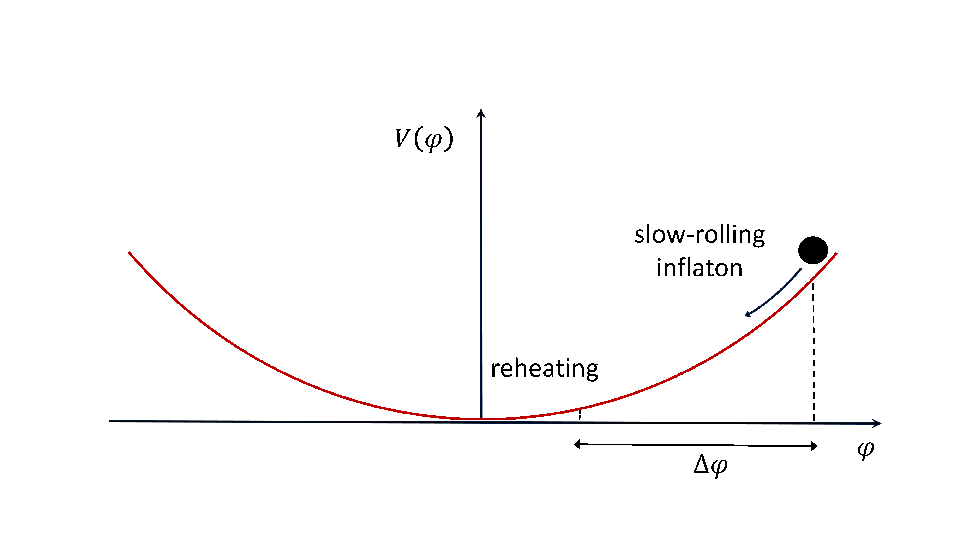
\includegraphics[width=0.55\linewidth, height=0.24\textheight]{Images/Chap2/ChaoticInflation_GWFromInflation_Fig3}
	\caption{Example of chaotic inflation potential. $ \Delta \phi $  indicates the inflaton excursion between the horizon exit of a given comoving scale and the end of inflation. Chaotic inflation is an example of \textit{large-field models} \cite{GWFromInflation:Intro}.}
	\label{fig:chaoticinflationgwfrominflationfig3}
\end{figure}
 Accounting for the expansion of the universe with Hubble constant $ H=\dot{a}/a $, the system is described by the equation of motion of the field $\phi$
\begin{equation}
	\label{Chap2eomChaoticInflation}
	\ddot{\phi} + 3H\dot{\phi} = -m^{2}\phi. 
\end{equation}
As said, the second term in the LHS of this equation can be interpreted as a friction term. The Friedmann equation (\ref{friedmannEquations1Chap2}) for a homogeneous universe containing the scalar field $\phi$, yields
\begin{equation}
	\label{Chap2:friedmannChaoticInflation}
	H^{2}=\frac{8 \pi G}{3}\rho_{\phi}= \frac{4 \pi G}{3}\Big (\dot{\phi}^{2} + m^{2}\phi^{2} \Big ),
\end{equation}
where we have used (\ref{energyDensityPressure}) and neglected the curvature term.

From the last equation we see that if the scalar field $\phi$ initially was large, the Hubble parameter $ H $ had to be large too and then the friction term. This means that the scalar field during inflation was moving very slowly, as a ball in a viscous liquid. Therefore, the energy density of the inflaton, unlike the density of ordinary matter, remained almost constant and the expansion of the universe continued with a high speed. 

Soon after the beginning of this regime (rapid expansion of the universe and slow motion of $\phi$) we obtain $ \ddot{\phi} \ll 3H\dot{\phi} $ and $\dot{\phi^{2}}$ $\ll$ $ m^{2}\phi^{2} $, yielding
\begin{equation}
	\label{Chap2:HubbleRateField}
	H=\frac{\dot{a}}{a} =\sqrt{\frac{4\pi G}{3}}m\phi.
\end{equation}
 This equation shows that if the field $\phi$ changes slowly, the size of the universe in this regime grows approximately as $ e^{H t} $ with $ H $ given by (\ref{Chap2:HubbleRateField}). 
 
 In this model inflation does not require initial state of thermal equilibrium, supercooling and tunnelling from the false vacuum. This means that, in this scenario, there is no bubble nucleation and then the problems seen with Guth's model are avoided.
 
 When inflation ends, the scalar field $\phi$ begins to oscillate near the minimun of $ V(\phi) $. As any rapidly oscillating classical field, it looses its energy by creating pairs of elementary particles. These particles interact with each other and come to a state of thermal equilibrium with some temperature $ T_{r} $. From this time on, the universe can be described by the usual Big-Bang theory.
 
 To have an idea of the huge expansion of the universe during inflation we can consider the mass $ m $ of the inflaton about $ 10^{-6} M_{p} $, and an initially closed universe with initial size $ l \simeq M_{p}^{-1} $. Moreover, we assume as initial condition for the energy density $\rho \simeq 1$ of the scalar field. From $\rho < 1$ we can consider this domain as classical universe.
 
 Solving (\ref{Chap2:HubbleRateField}) comes out that the total amount of inflation achieved starting from $ V(\phi) \simeq 1 $ is of the order of $ 10^{10^{10}} $ ! . In this model the total duration of inflation is about $ 10^{-30} $ seconds. From investigations of this period, if we consider the initial size of the universe small as the Planck size $ l_{p} $ $\simeq 10^{-33} cm$, after $ 10^{-30} $ seconds of inflation the universe acquires a huge size of $ l \simeq 10^{10^{10}} cm $ \cite{Chap2:Linde_HystoryInflation}. This value is model dependent, but in all realistic models  the size of the universe after inflation appears to be many orders of magnitude greater than the size of the part of the universe which we can see now, $ l \simeq 10^{28} cm $. Thus, most of the problems of the old cosmological theories are immediatly solved. 
 
 If the universe initially consisted of many domains with chaotically distributed scalar field $\phi$, then domains with a value of the inflaton too small never inflated. Thus, the main contribution is given by those domains which originally contained large scalar field $\phi$. Inflation of such domains creates very large homogeneous islands out of initial chaos, each one much greater than the size of the observable part of the universe.
 
 Other examples of models of chaotic inflation are based on polynomial potentials. The first potential proposed by Linde, when he suggested the chaotic inflation scenario, was $ V(\phi) = \frac{\lambda}{4} \phi^{4} $ \cite{ChaoticInflationLinde:Chap2}. However, the main idea of this type of inflation is quite generic. One can consider any particular potential $ V(\phi) $, polynomial or not, with or without spontaneous symmetry breaking, and study all possible initial conditions without assuming that the universe was in a state of thermal equilibrium. 
 
 \subsection{Small-field models}
 The small field models are characterized by the following potential around $\phi=0$:
 \begin{equation}
 	\label{Chap2:small-field1}
 	V(\phi) = V_{0}\Big [1-\Big (\frac{\phi}{\mu}\Big)^{n} \Big],
 \end{equation}
which may arise in spontaneous symmetry breaking.
An important example is \textit{Natural Inflation} model where a Pseudo Nambu-Goldstone boson (PNGB) playes the role of inflaton \cite{Chap2:NaturalInflation}. The PNGB potential is in  the form
\begin{equation}
	\label{Chap2:PNGBPotential}
	V(\phi) = \Lambda^{4}\big [1 + cos(\phi/f) \big],
\end{equation}  
 where the two mass scales $\Lambda$ and $ f $ characterize the height and width of the potential, respectevely (Fig. \ref{fig:naturalinflationinflationdynamics-and-reheating} from \cite{InflationDynamicsAndReheating:chap1}). The potential has a unique minimun at $ \phi = \pi f $. The typical mass scales for successful inflation are of order  $ f \sim M_{pl} \sim 10^{19} $ Gev and $ \Lambda \sim m_{GUT} \sim 10^{16} Gev $. For temperatures $ T \le f $ the global symmetry is spontaneously broken. These mass scales arise in particle physics models, for example in superstring theories. 
 
 \begin{figure}
 	\centering
 	\includegraphics[width=0.5\linewidth, height=0.25\textheight]{"Images/Chap2/NaturalInflation_InflationDynamics and reheating"}
 	\caption{Natural inflation potential. This is an example of \textit{small-field model} \cite{InflationDynamicsAndReheating:chap1}.}
 	\label{fig:naturalinflationinflationdynamics-and-reheating}
 \end{figure}
  We can describe the evolution of the field as 
 \begin{equation}
 	\label{Chap2:eomSmallFieldModel}
 	\ddot{\phi} + 3H\dot{\phi} + \Gamma\dot{\phi} + V'(\phi) = 0,
 \end{equation} 
where $\Gamma$ is the decay rate of the inflaton.
When the temperature T $\le$ $\Lambda$, in regions of the universe with $\phi$ initially near the top of the potential, the field starts to slowly roll down toward the minimum of the potential. In those regions the energy density of the universe is quickly dominated by the vacuum contribution and the universe expands exponentially. The slow-roll regime is characterized,  as in the previous models, by $ \ddot{\phi} \ll 3H\dot{\phi} $ and the initial conditions for the field $\phi$, as in chaotic scenario, are random. 

At the end of the slow-roll regime we have the reheating phase. The field $\phi$ begins to oscillate about the minimun of the potential and gives rise to particle and entropy production. 
During this process the energy of the inflaton is converted in radiation in a time $\simeq \Gamma^{-1}$. If $\Gamma > H$, then the reheating process takes less than an expansion time ($\simeq H^{-1}$) and the coherent field energy is efficiently converted into radiation, reheating the universe to a temperature \cite{Chap2:NaturalInflation_Turner_Steinhardt}
\begin{equation}
\label{Chap2:ReheatingTemperatureSmallFieldModel}
T_{RH}=\Big (\frac{45}{4\pi^{3}g_{*}}\Big )^{1/4} (Hm_{pl})^{1/2},
\end{equation}
where $ g_{*} $ counts the effective number of relativistic degree of freedom.

On the other hand, if $ \Gamma < H $, then the reheating process takes longer than an expansion time. Until $ t \simeq \Gamma^{-1} $ the field continues to oscillate about the minimun of the potential. When $ t \simeq \Gamma^{-1} $ these oscillations are damped (in a few expansion times), reheating the universe to a temperature
\begin{equation}
	T_{RH} \simeq \Big (\frac{45}{4\pi^{3}g_{*}}\Big)^{1/4}(\Gamma m_{pl})^{1/2}.
\end{equation}
The decay rate can be evaluated as 
\begin{equation}
	\label{Chap2:DecayRate}
	\Gamma \simeq g^{2}\Lambda^{6}/f^{5},
\end{equation}
where g is an effective coupling constant (for example, in the axion model \cite{Chap2:AxionModel}, $ g \propto \alpha_{EM} $ for two-photon decay). For $ f=m_{pl} $ and $ g_{*}=10^{3} $, we find that $ T_{RH} \simeq 10^{14}\ Gev $ in the first case ($ \Gamma > H $) and $ T_{RH} \simeq 10^{8} g\ Gev$ in the other case ($\Gamma < H$). Since generally we expect that $ g < 1 $, the reheating temperature will be $ T_{RH} < 10^{8}\ Gev $ \cite{Chap2:NaturalInflation}.
This can have very insteresting application in GUT baryogenesis models (see \cite{Chap2:NaturalInflation} and \cite{Chap2:NaturalInflation_Turner_Steinhardt}).

\subsection{Hybrid models}
In this type of model  inflation ends because of the combination of several scalar fields. In particular, we have a scenario with two interacting scalar fields where inflation ends by a rapid rolling (\textit{waterfall}) of a second scalar field $\sigma$ besides the inflaton, triggered by the slow rolling of the field $\phi$ \cite{Chap2: Hybrid_Model}.

An example of effective potential from this type of model is given by
\begin{equation}
\label{Chap2:Hybrid model}
	V(\sigma,\phi) = \frac{1}{4\lambda}(M^{2}-\lambda \sigma^{2})^{2} + \frac{m^{2}}{2}\phi^{2} + \frac{g^{2}}{2}\phi^{2}\sigma^{2} .
\end{equation} 
When the fields have large value their effective mass squared are both positive and the potential has the symmetry $ \sigma \leftrightarrow -\sigma $. The potential has a maximum at $\phi = \sigma = 0$ and a global minimum at $\phi = 0$, $\sigma=\sigma_{0}=M/\sqrt{\lambda }$ where the symmetry is broken.

The effective mass squared of the field $\sigma$ is obtained by deriving the potential two times with respect the field $\sigma$:
\begin{equation}
	\label{massEffectiveSigma}
	m^{2}_{\sigma} = V''_{\sigma}(\sigma,\phi) = -M^{2} + g^{2}\phi^{2}.
\end{equation}
 Since the curvature of the effective potential in the $\sigma$-direction is much greater than in the $\phi$-direction, we expect that at the first stages of expansion of the universe the field $\sigma$ rolled down to $\sigma=0$, whereas the field $\phi$ could remain large for longer time. Thus, we can consider the motion starting at large $\phi$ (where the effective mass of the $\sigma$ field is large), with the field  sitting at the minimum of the potential at $\sigma=0$.df
 
 During the slow-roll of the field $\phi$, the effective mass of the triggering field is $ m^{2}_{\sigma} = g^{2}\phi^{2}-M^{2}$. As soon as the field $\phi$ acquires the critical value $\phi_{c}=M/g$, fluctuations of the massless $\sigma$ field trigger the symmetry breaking phase and inflation ends. 
 
 \begin{figure}
 	\centering
 	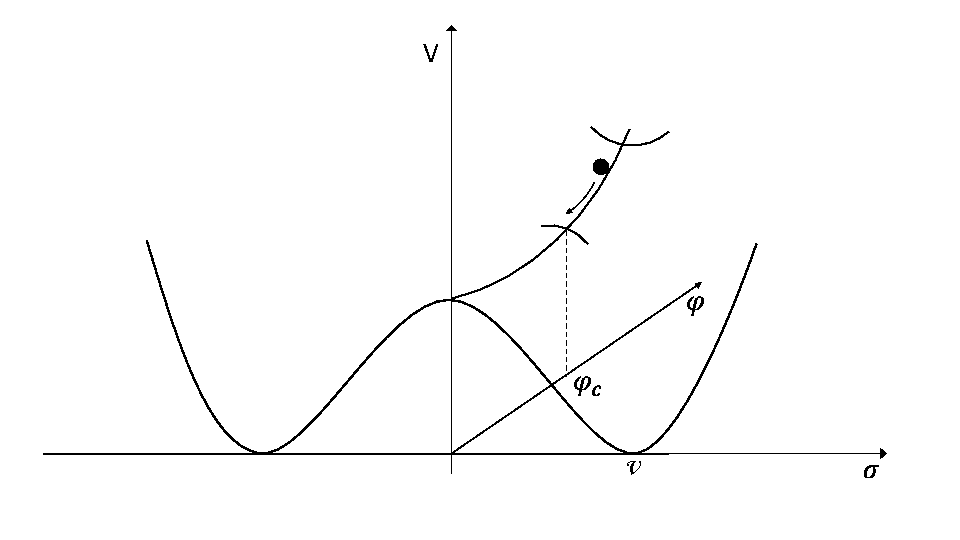
\includegraphics[width=0.55\linewidth, height=0.25\textheight]{Images/Chap2/HybridModel_GWFromInflation_Fig4}
 	\caption{Hybrid inflation potential. The field rolls down the potential up to the critical value $\phi_{c}$, and then reaches the true minimum of the potential $ \phi=0,\sigma=\sigma_{0}=v$ \cite{GWFromInflation:Intro}}
 	\label{fig:hybridmodelgwfrominflationfig4}.
 \end{figure} 
 If the bare mass $ M $ is large compared with the rate of expansion $H$ of the universe, the transition will be instantaneous and inflation will end very rapidly. Instead, if the $ M $ parameter is of the order of $ H $, then the transition will be very slow and we can have a few more e-folds of inflation after the phase transition. When $ \sigma=0 $ the effective potential becomes
 \begin{equation}
 \label{effectivePotential}
 V(\phi)=\frac{M^{4}}{4\lambda} +  \frac{m^{2} \phi^{2}}{2}.
 \end{equation}
Since during inflation the scalar field $\phi$ is of the order $\phi_{c}=M/g$, if $ m^{2} \ll g^{2}M^{2}/\lambda $ we obtain for the potential the expression
\begin{equation}
	\label{potential}
	V(\phi,0)=\frac{M^{4}}{4\lambda} +  \frac{m^{2} \phi^{2}}{2} \simeq \frac{M^{4}}{4\lambda},
\end{equation} 
and for the Hubble rate, under this condition,
\begin{equation}
	\label{Chap2:HubbleHybrid}
	H^{2}\simeq\frac{8\pi G}{3} V(\phi,0) \simeq \frac{8\pi }{3M_{pl}^{2}}\frac{M^{4}}{4\lambda} =\frac{2\pi M^{4}}{3\lambda M_{pl}^{2}}.
\end{equation}
This means that, under the condition $  m^{2} \ll g^{2}M^{2}/\lambda $, we obtain inflation for $ \phi > \phi_{c} $. In this case the inflation is driven by the vacuum energy density $ V(0,0) = M^{4}/4\lambda $.

The complete equation of motion of the field $\phi$ is
\begin{equation}
	\ddot{\phi} + 3H\dot{\phi}=-(m^{2} + g^{2}\sigma^{2})\phi.
\end{equation}
As said, during inflation $\sigma=0$ and one can neglect $\ddot{\phi}$ in the equation of motion for the field $\phi$, yielding
\begin{equation}
	\label{eom}
	3H\dot{\phi}=-m^{2}\phi.
\end{equation}
It is then possible to integrate the evolution equation of $\phi$, obtaining
\begin{equation}	
	\label{Chap2:solutionField}
	\phi(N)=\phi_{c}e^{rN} \qquad r\simeq \frac{m^{2}}{3H^{2}},
\end{equation}
where $ N=H(t_{c}-t) $ is the number of e-folds to the phase transition.

We can study the beheaviour of the fields $\phi$ and $\sigma$ after the time 
$ \Delta t = H^{-1}=\sqrt{\frac{3\lambda}{2\pi}}\frac{M_{pl}}{M^{2}} $, from the moment $ t_{c} $ when the field $\phi$ becomes equal to $\phi_{c}$.
Considering the equation of motion of the field during inflation (\ref{eom}), during the time $\Delta t$, the variation $\Delta \phi$ is
\begin{equation}
	\label{Chap2:variationDeltaPhi}
	\Delta \phi = \frac{m^{2} \phi_{c}}{3H^{2}} = \frac{m^{2}M}{3H^{2}g} = \frac{\lambda m^{2}M_{pl}^{2}}{2\pi gM^{3}}.
\end{equation}
Thus, the value of the field after $\Delta t$ becomes
\begin{equation}
	\label{Chap2:fieldSquare}
	\phi_{t_{c}-\Delta\phi}=\frac{M}{g}\Big (1-\frac{\lambda m^{2} M^{2}_{pl}} {2\pi M^{4}} \Big ).
\end{equation}
Moreover, after $ t_{c} - \Delta t $ the value of the negative mass squared of the field $\sigma$ (\ref{massEffectiveSigma}) becomes
\begin{equation}
	\label{Chap2}
	m^{2}_{\sigma} = - M^{2}(\phi) = - \frac{\lambda m^{2}M^{2}_{pl}}{\pi M^{2}}, 
\end{equation}
where the square of the field $\phi$ is obtained expanding the square of (\ref{Chap2:fieldSquare}) (we are working in the regime $ M^{2} \gg \lambda m^{2}/g^{2} $).

The value of $ M^{2}(\phi) $ is much greater than $ H^{2} $ for $ M^{3} \ll \lambda m M_{pl}^{2} $ (see (\ref{Chap2:HubbleHybrid})). This means that the field $\sigma$ within the time $\Delta t \sim H^{-1} $ rolls down to its minimum at $\sigma (\phi) = M(\phi)/\sqrt{\lambda}$, rapidly oscillates near it and loses its energy  due to the expansion of the universe.
It can be checked that the field $\phi$ rolls down very fast towards the minimum of its effective potential within a time much smaller than $ H^{-1} $ if $ M^{3} \ll \sqrt{\lambda}gmM_{pl}^{2} $.
Thus, under these conditions inflation ends in this theory almost instantaneously, as soon as the field $\phi$ reaches the critical value $\phi_{c} = M/g$.

Considering the reheating phase at the end of this type of model, it will be important the following consideration. According to the classical equation of motion, the field $ \sigma=0 $ cannot change its value because the first derivative of the effective potential at $\sigma=0$ vanishes. The spontaneous symmetry breaking,  in this case, occurs due to the exponential growth of quantum fluctuations. Indeed, writing the (negative) effective mass squared of the field $ -m^{2}_{\sigma}(\phi)=g^{2}(\phi-\phi_{c}) $, we immediately see that it vanishes at the critical point, but becomes large and grows up to $ m^{2}_{\sigma}(0) = M $ as the field $\phi$ slides towards $\phi=0$. This leads to a fast growing of quantum fluctuations of the scalar field $\sigma$, producing an inhomogeneous distribution of the field $\sigma$ with $ <\sigma>=0 $. We will return to this in a more detailed way later. 

Quantum fluctuations of the inflaton field produce metric perturbations $ \mathcal{R} \simeq H\delta\phi/\dot{\phi} $, where $\delta \phi$ is the amplitude of the field fluctuations when they cross outside the Hubble scale.
Appying (\ref{PR}) with the solution (\ref{Chap2:solutionField}) we obtain
\begin{equation}
\dot{\phi}=-(Hr\phi_{c})e^{rN},	
\end{equation}
and 
\begin{equation}
	\label{Chap2:P_{R}}
	P_{\mathcal{R}}=\Big (\frac{H^{2}}{4\pi^{2}r^{2}\phi_{c}^{2}}\Big)e^{-2rN} = \frac{1}{r^{2}}\frac{g^{2}M^{2}}{6\pi\lambda M_{pl}^{2}}e^{-2rN}.
\end{equation}
However, another more accurate way to compute this spectrum (\ref{Chap2:P_{R}}) is in \cite{Chap2:PerturbationsHybridInflation}. The only difference is that the spectrum (\ref{Chap2:P_{R}}) is multiplied by $ C(r)^{2} $ where $ C(r)=\Gamma[3/2-r]/2^{r}\Gamma[3/2] $ $\simeq 1$ in the limit $ m\ll H $.
Moreover, \cite{Chap2:PerturbationsHybridInflation} evaluated the spectral tilt as
\begin{equation}
	n_{\mathcal{R}} - 1 = \frac{d\ ln\ P_{\mathcal{R}}}{d\ ln\ k} = 2r. 
\end{equation}
Note that the tilt is always greater than one in this model.

Hybrid inflation is also a version of the chaotic inflation scenario. The main difference between this scenario and the simplest versions of the one-field chaotic inflation is in the way inflation ends. In the theory with  a single field inflation ends when the potential of this field becomes steep. In the hybrid picture, instead, inflation ends due to the presence of another scalar field that triggers the waterfall.
Several extensions of this scenario became quite popular in the context of supergravity and string cosmology.

\section{Observations}
Inflation is not just an interesting theory  that can resolve many problems of the standard Big-Bang Cosmology. The inflation paradigm made several predictions, which can be tested by cosmological observations.

The first important prediction is that the universe must be flat, and in most models $ \Omega = 1 \pm 10^{-4} $.
 An other important prediction is that  inflationary perturbations generated during a slow-roll regime with $\epsilon,\eta$ $\ll 1$ have a nearly flat spectrum with $ n_{S}$ close to 1. In general, the spectrum of inflationary perturbations usually is slightly non-flat. It is possibile to construct models with $ n_{S}$ extremely close (or even exactly equal) to 1, but the small deviation of the spectrum from the exact flatness is one of the distinguishing features of inflation.
 
 Perturbations of the metric could be scalar, vector or tensor. Inflation mostly produces scalar perturbations, but it also produces tensor perturbations with nearly flat spectrum, and it does not produce vector perturbations. As seen in the first chapter,  there are important relations between  scalar and tensor perturbations produced by inflation.
 The perturbations coming from inflation produce specific peaks in the spectrum of CMB radiation.
 It is possible to violate each of these predictions if one makes inflationary theory sufficiently complicated. For example, it is possible to produce vector perturbations of the metric in the models where cosmic strings are produced at the end of inflation, which is the case of some other models of hybrid inflation. However, it is difficult to do so, and most of the inflationary models obey the predictions above \cite{Chap2:Linde_HystoryInflation}.
 
 The most recent constraints on inflation comes from the 2018 $ Planck $ measurements of the CMB anisotropies \cite{Chap2:Planck2018}. The \textit{Planck} mission estimates the spectral index as
 \begin{equation}
 	\label{spectral index}
 	n_{s}= 0.9626 \pm 0.0057  \qquad (68\% C.L.),
 \end{equation}
and the curvature constraint
 \begin{equation}
 	\label{curvatureConstraint}
 	\Omega_{K}= 0.0007 \pm 0.0037 \qquad  (95\% C.L). 
 \end{equation}
Moreover, the tensor-to-scalar ratio $ r $ is estimated, assuming that it satisfies the consistency relation  ($ n_{T} = -r/8 $) \cite{Intro:ConstraintsOnr},
\begin{equation}
	r_{0.05} < 0.032 \qquad (95\% C.L.).
\end{equation}

To characterize the system we can write the power spectra w.r.t a pivot scale $ k_{0} $ as power laws
\begin{equation}
	\Delta_{T}(k) = \Delta_{T}(k_{0})\Big (\frac{k}{k_{0}}\Big)^{n_{T}} \qquad \Delta(k) = \Delta_{\zeta}(k_{0})\Big (\frac{k}{k_{0}}\Big)^{n_{s}-1},
\end{equation}
obtaining a set of 4 observables: 2 spectral indeces and 2 amplitudes.
Assuming the consistency relation true, we can reduce the DOF to 3.  Exploiting the normalitation of CMB anisotropies on large angular scales $ \Delta T/T \sim 10^{-5}$ \cite{Chap2:Wilkinson}, one can constraint one of the two amplitudes since it contains both $\zeta$ and GW contributions.
From experimental constraints on amplitudes and spectral indeces we can also constraint  the slow-roll parameters since $ n_{T}=-2\epsilon $ and $ n_{S}-1=2\eta - 6\epsilon $.

The usually chosen DOF to classify inflationary models are taken to be $ (r,n_{s}) $, from which we build the parameter space.
In the $ (r,n_{s}) $ plane we have that different classes of models (small-field, large-field, hybrid models) occupy different regions. Indeed, we can consider  the parameter $\eta\simeq M_{pl}V''/V$, and rewriting the tensor-to-scalar ratio in terms of the slow-roll parameters as $r=16\epsilon$, we obtain
\begin{equation}
	r(n_{s},\eta)=\frac{8}{3}(1-n_{s}) + \frac{2}{3\pi}M_{pl}^{2}\frac{V''}{V}.
\end{equation}
For $\eta < 0 $ we have small-field models, for $ 0<\eta<2\epsilon $ we have  large-field models and hybrid models provide $\eta>2\epsilon $. The hybrid models are almost excluded by observation yielding $ n_{s} \le 1 $.
As mentioned, even if we are considering only the simplest models which realise inflation, there is still a large variety of them ("zoology"). In addition, one can see that  large field models tend to produce more gravitational waves than small ones.
\begin{figure}
	\centering
	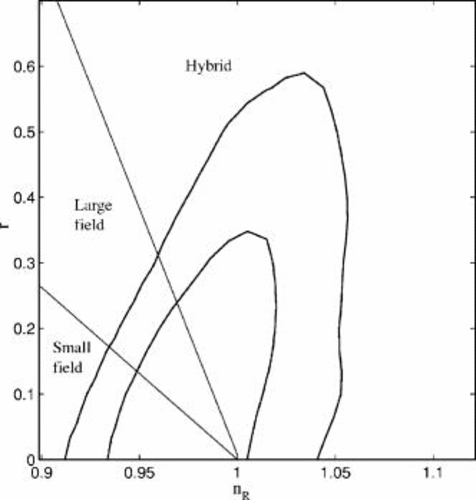
\includegraphics[width=0.6\linewidth, height=0.3\textheight]{Images/Chap2/r_ns_InflDynamicsAndReheating}
	\caption{Classification of inflationary models in the $ n_{\mathcal{R}}-r $ plane. The line $ r = (8/3)(1-n_{\mathcal{R}}) $ marks the border of large-field and small-field models,  whereas  the border of large-field and hybrid models correspond to $ r=8(1-n_\mathcal{R}) $ \cite{InflationDynamicsAndReheating:chap1}.}
	\label{fig:rnsinfldynamicsandreheating}
\end{figure}

\section{Reheating}
In this section we start to discuss one of the main focus of this thesis: the reheating stage after inflation.
As said, after  inflation the standard FLRW  radiation dominated universe should start in order to recover the standard Big-Bang model of the universe. However, during the accelerated expansion of the universe $ T \propto a^{-1} \simeq e^{-Ht} $. Then, at the end of inflation the temperature becomes too small to allow a good Thermalization of the particles, and then to start the radiation dominated era. This is the reason why we need a post-inflation period in which the universe is reheated, and which comes just before the radiation dominated era.
For now, we present a toy, elementary model of reheating. From Chapter 4 we will investigate deeply such a period and we will see, actually, that this phase leads to very interesting non-linear physics and dynamics. For reference see \cite{Chap2:Kolb_Turner}.
\begin{figure}
	\centering
	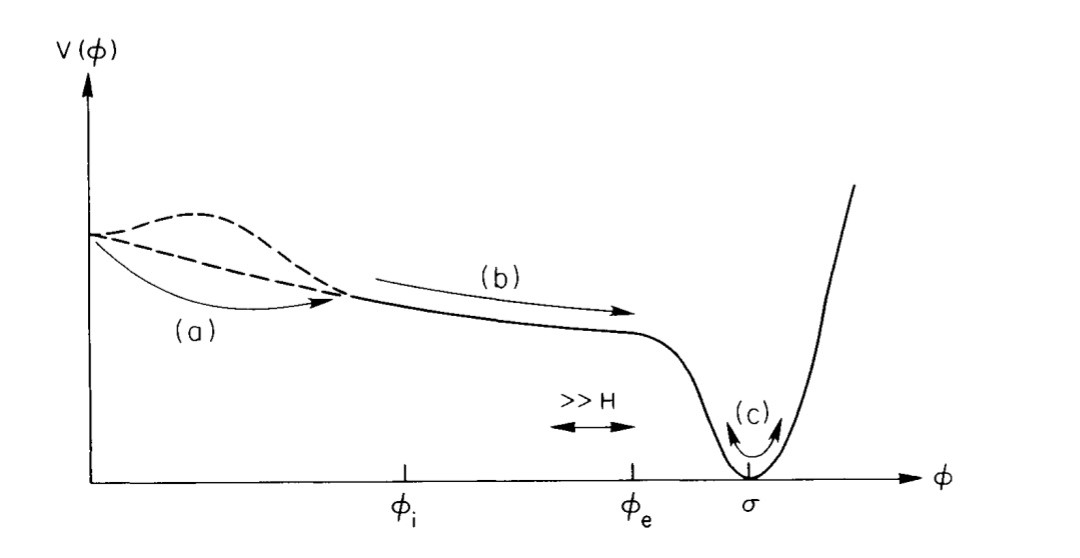
\includegraphics[width=0.8\linewidth, height=0.3\textheight]{Images/Chap1/ReheatingImage}
	\caption{Illustration of slow-roll inflation and reheating. In (a) we have barrier penetration (if needed); (b) is the stage of slow-roll; and (c) the coherent oscillations about the minimum of the potential \cite{Chap2:Kolb_Turner}.}
	\label{fig:reheatingimage}
\end{figure}

We start considering the simple single-field model discussed in the first chapter,
\begin{equation}
		\mathcal{L} = -\dfrac{1}{2} g^{\mu\nu} \partial_{\mu}\phi \partial_{\nu} \phi - V(\phi).
\end{equation}	
Inflation ends when the slow-roll parameter $\epsilon$ reaches the value 1, which implies that also $\eta=1$. Indeed, this happens when the curvature $ V'' $ of the potential starts to become non negligible, implying that the flat region in which the slow-roll takes place has ended. This stage is equivalent to say that $ V''\sim H^{2} $, that means $\eta \sim 1$ from (\ref{eta2}) (we recall that we have renamed $\eta_{V}$ as $\eta$). 

From this moment the second derivative of the potential starts to increase, becoming greater than the rate of the expansion of the universe, and the inflaton begins to oscillate around the minimum with a high frequency $\omega$. This leads to $ V'' \propto \omega^{2} \gg H^{2} $.
Moreover, the inflaton not only starts to oscillate with high frequency around the minimum of the potential, but it also decays with a rate $\Gamma_{\phi}$ to lighter relativistic particles that reheat the universe.

We can then modify the equation of motion for the inflaton field in a way that takes into account its decay,
\begin{equation}
	\label{Chap2:EOM_Modified}
	\ddot{\phi} + (3H + \Gamma_{\phi})\dot{\phi} + V'(\phi) = 0.
\end{equation}
We remark that the decay rate is a rate such as $H  $,  and then they should be multiplied by $\dot{\phi}$.
Consider now the energy density of the inflaton $\rho_{\phi} = \frac{1}{2} \dot{\phi^{2}} + V(\phi)$, and compute the time derivative
\begin{equation}
	\label{Chap2:dotPhi}
	\dot{\rho_{\phi}}=\dot{\phi}\ddot{\phi} + V'\dot{\phi}.
\end{equation}
Multiplying (\ref{Chap2:EOM_Modified}) by $\dot{\phi}$, and using the last expression, we obtain
\begin{equation}
	\label{Chap2:dotPhiEquation}
	\dot{\rho_{\phi}} + \dot{\phi^{2}}(3H^{2} + \Gamma_{\phi}) = 0.
\end{equation}
Moreover, using the fact that the typical time of oscillation is much smaller than the characteristic time of expansion, we can take an average over a period of oscillation such as
\begin{equation}
	\label{Chap2:oscillationAverage}
	\dfrac{1}{2} <\dot{\phi^{2}}>_{period}\ =\ <V(\phi)>_{period}\qquad \rightarrow\qquad \rho_{\phi}\ =\ <\dot{\phi^{2}}>_{period}.
\end{equation}
Finally, the final form of (\ref{Chap2:dotPhiEquation}) reads
\begin{equation}
	\label{Chap2:FinalEqRho}
\dot{\rho}_{\phi} + (3H + \Gamma_{\phi})\rho_{\phi} = 0	.
\end{equation}
To solve this equation, we consider the general solution
\begin{equation}
	\label{Chap2:rhoSolution1}
	\rho_{\phi}(t)=\rho_{osc}e^{-A(t)}, \qquad A(t)=\int_{t_{osc}}^{t}(3H+\Gamma_{\phi})dt,
\end{equation}
where $ \rho_{osc} $ denotes the initial condition at $ t_{osc} $, the time at which the inflaton begins to oscillate. The solution for $ A(t) $ reads
\begin{equation}
	\label{Chap2:solutionAt)}
	A(t)= \int_{t_{osc}}^{t}\Big (3 \frac{\dot{a}}{a} + \Gamma_{\phi}\Big) dt = 3 \ln \Big(\frac{a(t)}{a_{osc}}\Big) + \Gamma_{\phi}(t-t_{osc}),
\end{equation}
and substituing in (\ref{Chap2:rhoSolution1}), we finally obtain the solution
\begin{equation}
\label{Chap2:rhoSolution}
\rho_{\phi} = \rho_{osc} \Big (\frac{a}{a_{osc}}\Big)^{-3}e^{-(t-t_{osc})\Gamma_{\phi}}.	
\end{equation}
From this equation we obtain an interesting feature of this system: during the oscillation phase the inflaton beheaves as non-relativistic pressureless matter. Moreover, we can impose as initial condition $ \rho_{osc}=M^{4} $.
The exponential extra factor accounts for the decay of the field.
\begin{figure}
	\centering
	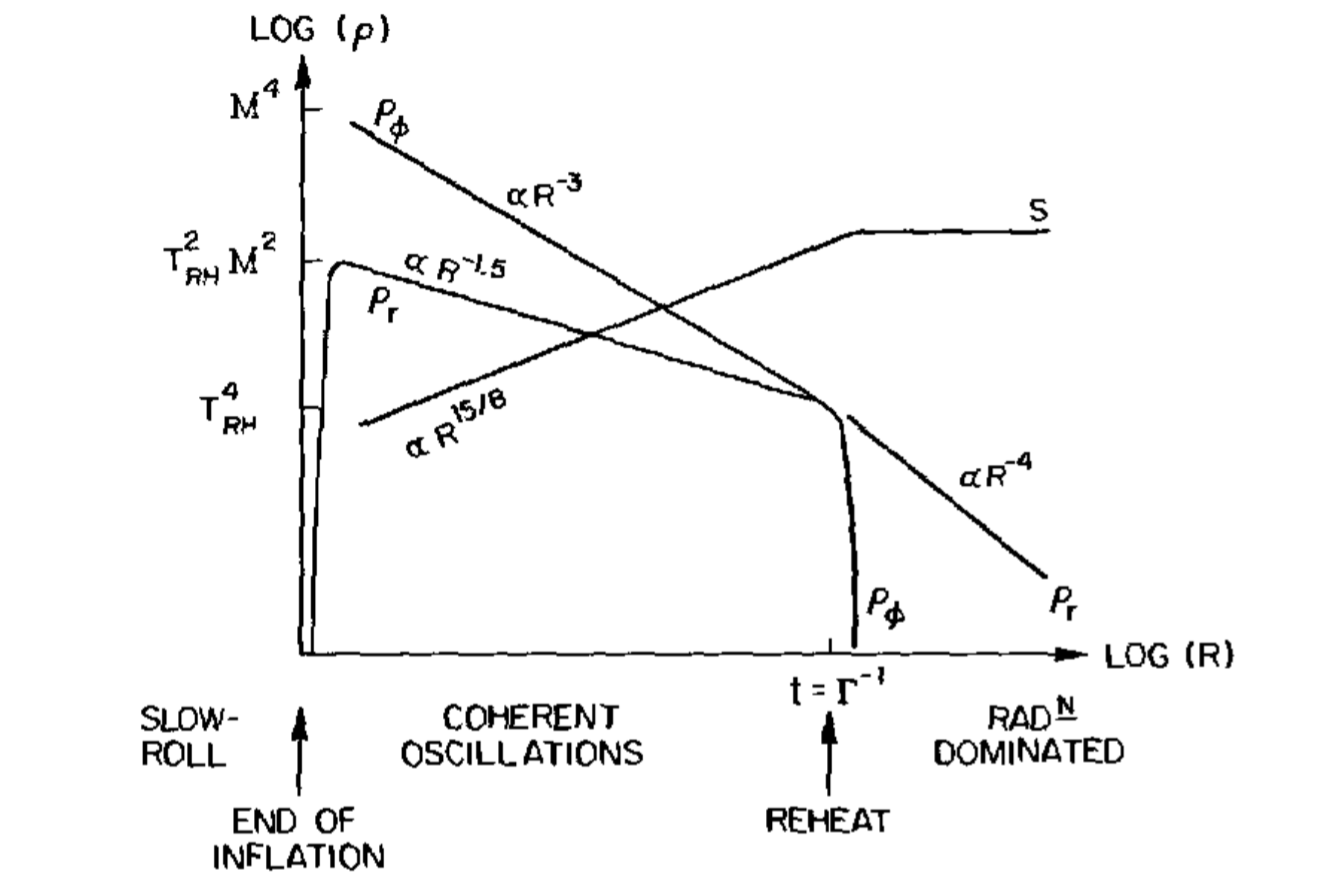
\includegraphics[width=0.8\linewidth, height=0.3\textheight]{Images/Chap2/EvolutionEnergyDensity}
	\caption{Summary of the evolution of $\rho_{\phi}$, $ \rho_{r} $ and $ S $ during reheating \cite{Chap2:Kolb_Turner}.}
	\label{fig:evolutionenergydensity}
\end{figure}

We can summarize the situation. After the end of inflation, as a consequence of the no-more negligible curvature of the potential, the inflaton field moves towards the minimum and starts to oscillate around it with  high frequency. At times $ t $ near to $ t_{osc} $ the decay of $\phi$ is not efficient and $\rho_{\phi}$ decreases essentially as $ a^{-3} $. However, the field $\phi$ starts to decay with a rate $\Gamma_{\phi}$. Because of these contributions the energy density of the inflaton decreases, but still dominates the energy density of the universe. As time passes, the decay starts to become important, and  at $ t_{decay} \sim 1/\Gamma_{\phi} $ becomes very efficient.
At this point the energy density of the inflaton starts to be very strongly suppressed and that of the relativistic particles increases (Fig. \ref{fig:evolutionenergydensity} from \cite{Chap2:Kolb_Turner}).

The presence of the new term $\Gamma_{\phi}$ related,  to the decay of the inflaton field, brings to a modification also to the equation for the energy density of radiation, which becomes
\begin{equation}
	\label{Chap2:radiationEquation}
	\dot{\rho_{r}} + 4H\rho_{r} = \Gamma_{\phi}\rho_{\phi}.
\end{equation}
As we said, from $ t_{osc} \simeq H^{-1} \simeq M_{pl}/M^{2} $ to $ t_{decay} \simeq \Gamma^{-1} $ the field oscillates but, although in principle it can decay, this process is still not efficient. Lighter particles begin to be produced in a slow way and their energy is still dominated by that of the inflaton, which energy continues to decrease.
As a consequence of this peculiar phase $\rho_{r}$ has not the particular beheaviour $ a^{-4} $, which is expected in the standard radiation dominated era, but the universe is still dominated by a matter-like field. In such a phase the scale factor evolves as $ a \propto t^{2/3} $ and the Hubble constant reads $ H=2/3t $.
Thus, starting from (\ref{Chap2:radiationEquation}) we can write
\begin{equation}
	\label{Chap2:radiationEquation2}
	\dot{\rho_{r}} + \frac{8}{3t}\rho_{r}\simeq \Gamma_{\phi}\rho_{osc}\Big (\frac{a}{a_{osc}}\Big)^{-3},
\end{equation}
where we have evaluated the expression near $ t_{osc} \sim M_{pl}/M^{2} $, neglecting the exponential term in $\rho_{\phi}$. Considering the time beheaviour of the scale factor  and $\rho_{osc}=M^{4}$, this equation yields
\begin{equation}
	\label{Chap2:radiation3}
		\dot{\rho_{r}} + \frac{8}{3t}\rho_{r} \simeq \Gamma_{\phi} M^{4} \Big (\frac{t}{t_{osc}}\Big)^{-2} \simeq \frac{\Gamma_{\phi} M_{pl}^{2}}{t^{2}}.
\end{equation}
To solve this equation we can search solution for $ \rho_{r} \propto t^{\alpha} $, taking as initial condition $\rho_{r}(t_{osc})=0$. We can use also the general solution
\begin{equation}
	\label{Chap2:generalSolution}
	\rho_{r}(t)=c_{in}e^{-A(t)} + e^{-A(t)} \int_{t_{osc}}^{t}dt'\ (g(t')e^{A(t')}), \qquad 
	g(t') = \frac{\Gamma_{\phi} M_{pl}^{2}}{t'^{2}}  ,
\end{equation}
where $ c_{in} $ denotes the initial condition. Putting $ \rho(t_{osc})=0 $, it is easy to see that $ c_{in}=0 $. The $ A(t) $ term is given by
\begin{equation}
	\label{Chap2:A(t)2}
	A(t)=\int_{t_{osc}}^{t}\frac{8}{3t'}dt'=\frac{8}{3}\ln(t/t_{osc}).
\end{equation}
Finally, the integral term in (\ref{Chap2:generalSolution}) yields
\begin{equation}
	\label{Chap2:IntegralTerm}
	\int_{t_{osc}}^{t} dt'\frac{\Gamma_{\phi} M_{pl}^{2}}{t'^{2}}\Big (\frac{t'}{t_{osc}}\Big)^{8/3} = \frac{9}{40}\frac{\Gamma_{\phi} M_{pl}^{2}}{t_{osc}^{8/3}}(t^{5/3} - t_{osc}^{5/3}).
\end{equation}
Putting all inside (\ref{Chap2:generalSolution}), we obtain
\begin{equation}
	\rho_{r}=\frac{9}{40}\frac{\Gamma_{\phi}M_{pl}^{2}}{t}\Big (1- \Big (\frac{t}{t_{osc}}\Big)^{-5/3}\Big).
\end{equation}
Using the scaling beheaviour $ a \propto t^{2/3} $, we can write the last expression in terms of the scale factor, obtaining the final solution
\begin{equation}
\label{Chap2:finalSolution}
\rho_{r}(t)=\frac{9}{40}\frac{\Gamma_{\phi}M_{pl}^{2}}{t_{osc}}\Big (\frac{a}{a_{osc}}\Big)^{-3/2}\Big (1- \Big (\frac{a}{a_{osc}}\Big)^{-5/2}\Big),
\end{equation}
and using $ t_{osc}=M_{pl}/M^{2} $,
\begin{equation}
	\rho_{r}(t)=\frac{9}{40}\Gamma_{\phi}M_{pl}M^{2}\Big (\frac{a}{a_{osc}}\Big)^{-3/2}\Big (1- \Big (\frac{a}{a_{osc}}\Big)^{-5/2}\Big).
\end{equation}
From this equation we can determine easily the beheaviour of the radiation energy density. During the period of oscillation of the inflaton field the radiation energy starts to grow from zero up to a maximum value $\rho_{max} \simeq \Gamma_{\phi} M_{pl} M^{2}$, thanks to the inflaton decays. Once the maximum is reached, $\rho_{r}$ decreased as $ a^{-3/2} $, instead of the usual $ a^{-4} $.

Regarding the temperature, we can estimate the maximum temperature reached by the radiation fluid at $\rho_{max}$ using $ \rho_{r}=(\pi^{2}/30)g_{*}T^{4} $. We obtain 
\begin{equation}
	T_{max} \sim g_{*}^{-1/4}(\rho_{r}^{max})^{1/4} \sim g_{*}^{-1/4}\Gamma_{\phi}^{1/4}M_{pl}^{1/4}M^{1/2}.
\end{equation}
During this phase the system  is still between the start of oscillations and the time at which decays become efficient. In such a period we have that also the entropy increases. Indeed, the total entropy $ S = sa^{3} $ is constant only if the entropy density scales as $ s \propto a^{3} $. This happens only in a pure FLRW radiation dominated universe, and we are not yet in that phase.
In this period 
\begin{equation}
\label{Chap2:entropy}
s \propto T^{3} \sim \rho_{r}^{3/4} \sim a^{-9/8},
\end{equation}
that leads
\begin{equation}
	\label{Chap2:totalEntropy}
	S \propto a^{15/8}.
\end{equation}
Thus, during this stage the inflaton decays producing new relativistic particles and this process causes the increasing of the entropy.

In the final stage we reach the time $ t_{decay} \sim \Gamma^{-1}_{\phi} $. From this moment the decay of the inflaton is efficient due to the exponential term in (\ref{Chap2:rhoSolution}). The energy density of the field $\rho_{\phi}$ decreases rapidly and $\rho_{r}$ becomes the dominant energy density, allowing to recover the usual radiation dominated era in which $ \rho_{r} \propto a^{-4} $ and $ S=const $. The temperature at which the radiation energy becomes the dominant energy of the universe (and then when the radiation dominated era begins) is called \textit{Reheating Temperature} $ T_{R} $. To estimate this temperature we can consider the Hubble constant during the standard radiation dominated era, and evaluating it at $ t_{decay}=\Gamma_{\phi}^{-1} $, we obtain
\begin{equation}
	\label{HubbleConstant}
	H^{2} = \Big (\frac{1}{2t}\Big)^{2} = \frac{\Gamma_{\phi}^{2}}{4} ,
\end{equation}
and
\begin{equation}
	H^{2}=\frac{8\pi }{3M_{pl}^{2}}\rho_{r}\simeq \frac{8 \pi g_{*}}{3M_{pl}^{2}}\frac{\pi^{2}}{30}T^{4}_{\ |t\simeq \Gamma_{\phi}^{-1}}.
\end{equation}
Combining the last two equations, we finally derive an estimate of the reheating temperature,
\begin{equation}
	\label{Chap2:reheatingTemperature}
	T_{R} \simeq 0.55g_{*}^{1/4}(\Gamma_{\phi}M_{pl})^{1/2},
\end{equation}
where we assumed for semplicity that the radiation dominated era starts at the instant $ t_{decay} $, when the decay of the inflaton field becomes efficient.
 
As final comment, we notice that there is no remnant of the vacuum energy density of the inflaton field, which drives the accelerated expansion of the universe. Indeed, just after inflation, $\phi$ beheaves as a non-relativistic pressureless field which causes its redshifting as $ a^{3} $.

There is also a special case in which the reheating is istantaneous at $ \rho_{osc} \simeq M^{4} \simeq T^{4}_{R} $. This happens when at $ t_{osc} $ the decay of the inflaton field is already extremely efficient. $\phi$ will not even make a single oscillation around the minimum, transforming immediately all the vacuum energy directly into radiation. In this special case we have $ T_{R} \simeq M $.

\chapter{Reheating Observables}
Detection of the stochastic background of primordial gravitational waves would have profound implications for the physics of the early universe and the high energy physics. The fundamental reason why gravitational waves carry information about the very early universe is that particles which decoupled from the primordial plasma at a certain time $ t\sim t_{dec} $, when the universe had a temperature of $ T_{dec} $, memorize the physical state of the universe at $ T_{dec} $. Since gravitons decoupled below the Planck energy scale, they memorize all the expansion history of the universe after they decoupled  allowing us to see through the entire history of the universe. Another example are CMB photons which decoupled from matter at $ T\sim 0.3 $ eV. However, the primordial gravitational waves carry information on the state of the much earlier universe than CMB photons do.

As discussed in the first chapter, the primordial gravitational waves spectrum would also provide informations about inflation and reheating. Indeed, the energy scale of inflation is directly related to the amplitude of the spectrum. Typically, the amplitude of the spectrum is of order $ 10^{-15} $ for $ 10^{16} $ GeV inflation energy scale. Inflation ends when the inflaton decays into radiation and reheats the universe. The energy scale of reheating could be seen from the highest frequency end of a nearly scale invariant energy density spectrum. The modes which re-entered the horizon during the radiation dominated era show a nearly scale invariant spectrum if we don't consider the change of the effective number of degrees of freedom.

The slope of the spectrum provides the power-law index of the tensor perturbation $ n_{T} $. $ n_{T}=0 $ corresponds to a scale invariant power spectrum from purely de-Sitter inflation. In a large class of inflationary models the absolute value of $ n_{T} $ is not zero but much smaller than unity, and its determination constraints the inflationary models. Thus, the  primordial gravitational waves not only test and probe the physics of inflation and reheating, but also the study of the spectrum enables us to probe the very early universe in a transparent way \cite{Chap3:GW_Watanabe_Komatsu}.

The universe is transparent to GW up to the Planck epoch in principle, and then we can obtain informations about the reheating epoch. Although the GW amplitude is constant  in the super-horizon regime, once a mode enters the horizon again it is reduced as the universe expands. Since the expansion rate depends on the equation of state of the universe, corresponding thermal history of the universe is imprinted in the gravitational wave spectrum at present.

In particular, the reheating stage is characterized by the reheating temperature $ T_{R} \sim g_{*}^{1/4}(\Gamma_{\phi}M_{pl})^{1/2} $, that we have estimated in the simple reheating model in the previous chapter. $ T_{R} $ is hardly constrained from cosmological observations by now. However, the reheating temperature contains rich information from the viewpoints of particle physics. Indeed, it is determined by the inflaton decay rate, and it depends on the inflaton properties, such as its mass, potential and the interaction strength with other particles. Thus, determining  $ T_{R} $ may have impacts on choosing realistic inflation models and inflaton candidates. In the first part of this chapter we consider how the detection of the primordial gravitational wave background produced in the inflationary era can determine the thermal history of the universe before Big-Bang Nucleosynthesis (BBN), in particular the reheating temperature $ T_{R} $. We will also discuss how the gravitational wave spectrum changes with some non-standard cosmological scenarios, as late-time entropy production during reheating.
In the second part we will study how we can obtain informations about reheating from measurements of CMB.
\section{Energy Density of GW}
In the first chapter we derived a solution for the gravitational waves. In this section we define the  spectral energy density $\Omega_{GW}$ of the gravitational wave background relative to the power spectrum $ P^{2}_{h}(k)$. In accordance with the literature, we rename the power spectrum of the gravitational waves as $ \Delta_{T} $ and the power spectrum of curvature perturbations as $\Delta_{\zeta}$.
\subsection{The transfer function}
Consider the equation of the gravitational waves for the mode \textbf{k},
\begin{equation}
	\ddot{h}_{\lambda,\textbf{k}} + 3H\dot{h}_{\lambda,\textbf{k}}+ k^{2}\frac{h_{\lambda,\textbf{k}}}{a^{2}}=0.
\end{equation}
we can express it in terms of the conformal time,
\begin{equation}
	\label{Chap3:equationGWConformalTime}
	h''_{\lambda,\textbf{k}} + \Big (\frac{2a'}{a}\Big)h'_{\lambda,\textbf{k}} + k^{2}h_{\lambda,\textbf{k}} = 0.
\end{equation}
This is just the massles Klein-Gordon equation for a plane wave in an expanding universe. Each polarization state of the wave behaves as a massless, minimally coupled, real scalar field. 

After the fluctuations left the horizon, $ k \ll aH $, (\ref{Chap3:equationGWConformalTime}) becomes
\begin{equation}
	\label{Chap3:solutionEquationConformalTime1}
	\frac{h''_{\lambda,\textbf{k}}}{h'_{\lambda,\textbf{k}}} \simeq -2 \frac{a'}{a}, 
\end{equation}
whose solution is
\begin{equation}
	\label{Chap3:solutionGWEquationConformalTime2}
	h_{\lambda,\textbf{k}}(\tau)=A + B \int_{}^{\tau}\frac{d\tau '}{a^{2}(\tau)},
\end{equation}
where A and B are integration constants. Discarding the second term, which is a decaying mode, we obtain that $ h_{\lambda,\textbf{k}} $ remains constant outside the horizon. Therefore, we can write a general solution of $ h_{\lambda,\textbf{k}} $ at any time as 
\begin{equation}
	\label{Chap3:transferFunction}
	h_{\lambda,\textbf{k}}(\tau) \equiv h_{\lambda,\textbf{k}}^{^{prim}}T(\tau, k),
\end{equation}
where $ h^{prim}_{\lambda,\textbf{k}} $ is the primordial gravitational wave mode that left the horizon during inflation. The transfer function $ T(\tau,k) $ then describes the sub-horizon evolution of GW modes after they  entered the horizon, and it is normalized such that $T (\tau,k) \rightarrow 1 $ as $ k \rightarrow 0$. The power spectrum of the gravitational waves $\Delta_{T}$ is defined as
\begin{equation}
	\langle h_{ij}(\lambda,\textbf{x})h^{ij}(\lambda,\textbf{x})\rangle = \int \frac{dk}{k}\Delta_{T}^{2}(\tau,\textbf{k}) = \frac{2k^{3}}{2\pi^{2}}\sum_{\lambda}\langle|h_{\lambda,\textbf{k}}(\tau)|^{2}\rangle.
\end{equation}
Using (\ref{Chap3:transferFunction}), one can write the power spectrum as 
\begin{equation}
	\label{Chap3:powerSpectrumTransferFunction}
	\Delta_{T}^{2}(\tau,k) \equiv \Delta^{2}_{T,prim}[T(\tau,k)]^{2},
\end{equation}
where
\begin{equation}
	\label{Chap3:DeltaTPrim}
\Delta_{T,prim} = \frac{2k^{3}}{2\pi^{2}}\sum_{\lambda}\langle|h^{prim}_{\lambda,\mathbf{k}}|^{2}\rangle = \frac{16}{\pi} \Big (\frac{H_{inf}}{M_{pl}}\Big)^{2}.
\end{equation}

\subsection{The spectral density $\Omega_{GW}(k)$}
The next step is to calculate the energy density of the gravitational waves, which is given by the (0-0) component of the stress-energy tensor. For reference of this section see \cite{Chap3:GW_Watanabe_Komatsu},\cite{Chap3: Gravitation}.

To obtain the energy momentum tensor of the gravitational waves consider the Ricci tensor of the FLRW metric (\ref{metric}), and expand it in metric perturbations, $ h $:
\begin{equation}
	\label{Chap3:RicciTensorExpansion}
	R_{\mu\nu} = \bar{R} + R^{(1)}_{\mu\nu} + R^{(2)}_{\mu\nu} + \mathcal{O}(h^{3}),
\end{equation}
where  $ R^{(1)}_{\mu\nu} \sim \mathcal{O}(h) $ and $ R^{(2)} \sim \mathcal{O}(h^{2}) $. In  vacuum we have $ R_{\mu\nu} = 0 $. Then, the linear term in (\ref{Chap3:RicciTensorExpansion}) must obey the vacuum equation,
\begin{equation} 
\label{Chap3:linearVacuumEquation}
	R^{(1)}_{\mu\nu} = 0.
\end{equation}
This is an equation for the propagation of the GW. The remaining part of (\ref{Chap3:RicciTensorExpansion}) in general is not linear in $ h_{\mu\nu} $, and can be divided into a smooth part which varies only on scales larger than some coarse-graining scales
\begin{equation}
	\label{Chap3:EqRicciTensor}
	\bar{R}_{\mu\nu} + \langle R_{\mu\nu}^{(2)} \rangle = 0, 
\end{equation}
and a fluctuating part which varies on smaller scales
\begin{equation}
	\label{Chap3:RicciEquationFluctuating part}
	R_{\mu\nu}^{(1)nonlinear} + R^{(2)}_{\mu\nu} - \langle R^{(2)}_{\mu\nu}\rangle = 0,
\end{equation}
up to second order in $ h_{\mu\nu} $. Here, $ R_{\mu\nu}^{(1)nonlinear}  $ is defined in this equation and represents the non-linear correction to the propagation of $ h_{\mu\nu} $ (\ref{Chap3:linearVacuumEquation}) (see \cite{Chap3:GW_Watanabe_Komatsu},\cite{Chap3: Gravitation}).

We can write the Einstein equation in vacuum as
\begin{equation}
\label{Chap3:RGEquation}
\bar{G}_{\mu\nu} = \bar{R}_{\mu\nu} - \frac{1}{2}\bar{R}\bar{g}_{\mu\nu} = 8\pi G T_{\mu\nu}^{(GW)},
\end{equation}
where
\begin{equation}
	\label{Chap3:TGWEquation}
	T_{\mu\nu}^{(GW)} \equiv -\frac{1}{8\pi G}\Big (\langle R^{(2)}_{\mu\nu}\rangle  - \frac{1}{2}\bar{g}_{\mu\nu}\langle R^{(2)}\rangle \Big)
\end{equation}
is a definition of the energy-momentum tensor for the gravitational waves, and $ \langle\cdot\rangle $ denotes an average over several wavelengths. The importance of the energy-momentum tensor is that it tells us how \textit{backreaction} from energy density of gravitational waves would affect the expansion law of the background universe. Since $ \langle R^{(2)}\rangle = 0 $ \cite{Chap3: Gravitation},
\begin{equation}
	\label{Chap3:TGW2}
	T_{\mu\nu}^{(GW)} = \frac{1}{32\pi G}\langle h_{\alpha\beta|\mu}h^{\alpha\beta}_{|\nu} \rangle  = \frac{1}{32\pi G} \langle h_{\alpha\beta,\mu} h^{\alpha\beta}_{,\nu} \rangle
	 + \mathcal{O}(h^{3}),
\end{equation}
where $ | $ is the covariant derivative with respect to the background metric, $\bar{g}_{\mu\nu} $. We have employed the transverse-traceless (TT) gauge and neglected higher order terms in the energy-momentum tensor.

The energy density of gravitational waves, $ \rho_{h} $, is defined by the (0-0) component of the energy momentum tensor
\begin{equation}
	\label{Chap3:energydensity}
	\rho_{h} \equiv T_{00}^{(GW)} = \frac{1}{32\pi G} \langle\dot{h}_{ij}\dot{h}^{ij}\rangle  ,
\end{equation}
where $ h_{ij} $ is in the TT gauge. We have only two independent modes for the GW:
\begin{equation}
	\label{Chap3:GWMatrix}
	h_{ij} = \left(
	\begin{array}{ccc}
		h_{+} & h_{\times} & 0 \\
		h_{\times} &- h_{+} & 0 \\
		0 & 0 & 0
	\end{array}
	\right),
\end{equation}
where $ + $ and $ \times $ denote the two independent polarization modes, and the propagation of the wave is taken in the $ \hat{z} $ direction.

Thus, from (\ref{Chap3:energydensity}) we obtain
\begin{equation}
	\label{Chap3:energydensity2}
	\rho_{h} = \frac{2}{32\pi G}\langle \dot{h}^{2}_{+} + \dot{h}^{2}_{\times}\rangle  = \frac{1}{16\pi G a^{2}}\langle h'^{\ 2}_{+} + h'^{\ 2}_{\times}\rangle   ,
\end{equation}
where we have expressed it in terms of the conformal time. The Fourier transformation of the last equation yields

\begin{equation}
\label{Chap3:EnergyDensityFourierTransform}
\rho_{h}=	\frac{1}{16\pi G a^{2}} \int \frac{d^{3}k}{(2\pi)^{3}}\int \frac{d^{3}k'}{(2\pi)^{3}} \langle (h_{+,\textbf{k}}'h_{+,\textbf{k}'}' + h_{\times,\textbf{k}}'h_{\times,\textbf{k}}')e^{i(\textbf{k} + \textbf{k}') \cdot \textbf{x}} \rangle  ,
\end{equation}
where $ h^{*}_{\lambda,\textbf{k}}=h_{\lambda,-\textbf{k}} $ is used. For stochastic modes the spatial average over several wavelengths, $ \langle  \rangle   $, is equivalent to the ensemble average in k space:
\begin{equation}
	\label{Chap3:ensembleAverage}
	\langle h'_{\lambda,\textbf{k}}h'_{\lambda',\textbf{k'}}\rangle  =(2\pi)^{3}\delta_{\lambda\lambda'}\delta^{(3)}(\textbf{k}+\textbf{k'})|h'_{\lambda,k}|^{2},
\end{equation}
where $\lambda = +,\times$. Inserting the last equation in (\ref{Chap3:EnergyDensityFourierTransform}), we obtain
\begin{equation}
	\rho_{h}(\tau)=\frac{1}{16\pi G a^{2}} \int \frac{d^{3} k}{(2\pi)^{3}}[|h'_{+,k}(\tau)|^{2} + |h'_{\times,k}(\tau)|^{2}].
\end{equation}
We assume that the primordial gravitational waves are unpolarized, i.e. $ |h'_{+,k}(\tau)|^{2} = |h'_{\times,k}(\tau)|^{2} $. Whenever we express the time evolution of some quantitities, it is convenient to express them in terms of the transfer function $T(k\tau)$.  The primordial amplitude $\Delta_{T,prim}^{2}$ defined in (\ref{Chap3:DeltaTPrim}) then reads
\begin{equation}
	\label{Chap3:EnergydensityTransferFunction}
	\rho_{h}(\tau)=\frac{1}{32\pi Ga^{2}}\int d\ln k\ \Delta_{T,prim}[T'(k\tau)]^{2},
\end{equation}
with 
\begin{equation}
	\label{Chap3:deltah2}
	\Delta_{T,prim}=4\frac{k^{3}}{2\pi^{2}}|h^{prim}_{k}|^{2}=\frac{16}{\pi}\Big(\frac{H_{inf}}{M_{pl}}\Big)^{2},
\end{equation}
where $|h^{prim}_{k}|^{2}  $ is the amplitude of gravitational waves outside the horizon, $ |k\tau| \ll 1 $, during inflation. 

It is common to define the relative spectral density as the normalized energy density per logarithmic scale
\begin{equation}
	\label{Chap3:relativeSpectralDensity}
	\Omega_{GW}(\tau,k) = \frac{\tilde{\rho_{h}}(\tau,k)}{\rho_{cr}(\tau)},
\end{equation}
with
\begin{equation}
	\label{Chap3:rhoTilde}
	\tilde{\rho_{h}}(\tau,k)=\frac{d \rho_{h}(\tau,k)}{d\ ln\ k},
\end{equation}
where $ \rho_{cr}(\tau) $ is the critical density of the universe, and $ \tilde{\rho_{h}}(\tau,k) $ denotes the energy density of the gravitational waves per logarithmic scale. Inserting (\ref{Chap3:EnergydensityTransferFunction}) into (\ref{Chap3:relativeSpectralDensity}), we obtain
\begin{equation}
	\label{Chap3:RelativeSpectralDensity_TransferFunction}
	\Omega_{GW}(\tau,k) = \frac{\Delta_{T,prim}^{2}}{32\pi Ga^{2}\rho_{cr}(\tau)}[T'(\tau,k)]^{2}.
\end{equation}
Finally, using the Friedmann equation $ H^{2}=8\pi G \rho_{c}/3 $, the final expression for the relative spectral energy density reads
\begin{equation}
	\label{Chap3:spectralDensityFinal}
		\Omega_{GW}(\tau,k) = \frac{\Delta_{T,prim}^{2}}{12H^{2}(\tau)a^{2}(\tau)}[{T'(\tau,k)}]^{2}.
\end{equation}
\subsection{Analytical solutions}
We can find  analytical solutions of (\ref{Chap3:equationGWConformalTime}) for the inflationary (assuming de-Sitter), radiation and matter dominated era \cite{Chap3:GW_Watanabe_Komatsu}.

From (\ref{Chap3:equationGWConformalTime}) we obtain the equation 
\begin{equation}
	\label{Chap3:eomMasslessDesitter}
	u''_{k}(\tau) + \Big[k^{2} - \frac{a''}{a}\Big]u_{k}(\tau) = 0,
\end{equation}
found in the first chapter (we remind that $ u_{k}(\tau) = h_{k}(\tau)/a(\tau) $). Using the fact that in a de-Sitter universe $ a''/a = 2/\tau^{2}  $, we obtain
\begin{equation}
	\label{eomMasslessDesitter2}
	u''_{k}(\tau) + \Big[k^{2} - \frac{2}{\tau^{2}}\Big]u_{k}(\tau) = 0.
\end{equation}
In this case we can find the exact solution 
\begin{equation}
	\label{Chap3:exactSolutionGWDeSitter}
	u_{k}(\tau) = c_{1}(k) \frac{e^{-ik\tau}}{\sqrt{2k}}\Big (1-\frac{i}{k\tau}\Big) + c_{2}(k) \frac{e^{ik\tau}}{\sqrt{2k}}\Big (1+\frac{i}{k\tau}\Big).
\end{equation}
Assuming the appropriate normalitation $ \lim_{\tau \rightarrow -\infty} u_{k}(\tau) = e^{-ik\tau}/\sqrt{2k}$ (positive frequency solution), (\ref{Chap3:exactSolutionGWDeSitter}) yields
\begin{equation}
	\label{Chap3:solutionBunchDavis}
h_{k}(\tau)= \frac{e^{-ik\tau}}{\sqrt{2k}a}\Big (1-\frac{i}{k\tau}\Big).
\end{equation}
For the radiation and matter dominated era we can recast (\ref{Chap3:equationGWConformalTime}) in the spherical Bessel functions. Indeed, considering that in the radiation era (RD) $\mathcal{H}= a'/a = 1/\tau$, and in the matter dominated era (MD) $\mathcal{H}=a'/a=2/\tau$, we obtain
\begin{equation}
	\label{Chap3:RadiationEra}
		h''_{\lambda,\textbf{k}} + \Big (\frac{1}{\tau}\Big)h'_{\lambda,\textbf{k}} + k^{2}h_{\lambda,\textbf{k}} = 0,
		\qquad
		RD
\end{equation}
\begin{equation}
	\label{Chap3:MatterEra}
	h''_{\lambda,\textbf{k}} + \Big (\frac{2}{\tau}\Big)h'_{\lambda,\textbf{k}} + k^{2}h_{\lambda,\textbf{k}} = 0.
	\qquad
	MD
\end{equation}
 We recognise in these equations the spherical Bessel equation after making the change of variables $ x\equiv k\eta $ and $ h\equiv f(x)/x $,
\begin{equation}
	\label{BesselFunction}
	x^{2}\frac{d^{2}f}{dx^{2}} + 2x\frac{df}{dx} + (x^{2} - l(l+1))f = 0,
\end{equation}
where $ l=0 $ in the case of radiation era, and $ l=1 $ in the matter era. The solution is given by $ f(x) = j_{l}(x) $.  Then the complete solution, accounting for the boundary conditions at the horizon crossing, is
\begin{equation}
	\label{Chap3:solutionRadiationEra}
	h_{\textbf{k}}(\tau)=[j_{0}(k\tau)]h_{\textbf{k}}^{prim}
	\qquad
	RD,
\end{equation}
\begin{equation}
	\label{Chap3:solutionMatterEra}
	h_{\textbf{k}}(\tau) = \Big [\frac{3 j_{1}(k\tau)}{k\tau}\Big] h_{\textbf{k}}^{prim}
	\qquad
	MD,
\end{equation}
where $ h_{\textbf{k}}^{prim} $ is evaluated at the horizon crossing.
Notice that $ |h_{k}(\tau)|^{2} $ in (\ref{Chap3:solutionBunchDavis}), (\ref{Chap3:RadiationEra}) and (\ref{Chap3:MatterEra}) does not depend on time at the super-horizon scale $ |k\tau| \ll 1$  ($ |h_{k}(\tau)|^{2} \simeq|h_{k}^{prim}|^{2} $).\\
Now, we classify wave modes by their horizon crossing time  $\tau_{hc}$: 
 $ |\textbf{k}|= k > k_{eq} $ denotes the modes that entered the horizon during RD ($ \tau_{hc} < \tau_{eq} $), while $ k < k_{eq} $ are the modes that entered the horizon during MD ($ \tau_{hc} > \tau_{eq} $). Using the transfer function (\ref{Chap3:transferFunction}), we obtain the time evolution of the amplitude of gravitational waves \cite{Chap3:GW_Watanabe_Komatsu}:
 \begin{equation}
 	\label{Chap3:TF1}
 	T(\tau < \tau_{eq}, k>k_{eq}) = j_{0}(k\tau),
 \end{equation}
\begin{equation}
	\label{Chap3:TF2}
     T(\tau > \tau_{eq}, k > k_{eq}) = \frac{\tau_{eq}}{\tau}[A(k)j_{1}(k\tau) + B(k)y_{1}(k\tau)],
\end{equation}
\begin{equation}
	\label{Chap3:TF3}
	T(\tau,k<k_{eq}) = \frac{3j_{1}(k\tau)}{k\tau},
\end{equation}
where
\begin{equation}
\label{Chap3:A(k)}
A(k) = \frac{3}{2k\tau_{eq}}-\frac{\cos(2k\tau_{eq})}{2k\tau_{eq}} + \frac{\sin(2k\tau_{eq})}{(k\tau_{eq})^{2}} ,
\end{equation}
\begin{equation}
	\label{Chap3:B(k)}
	B(k) = -1 + \frac{1}{(k\tau_{eq})^{2}} - \frac{\cos(2k\tau_{eq})}{(k\tau_{eq})^{2}} - \frac{\sin (2k\tau_{eq})}{2k\tau_{eq}},
\end{equation}
and $ y_{n} $ are the spherical Neumann functions. The conformal time derivatives  of the transfer functions are
\begin{equation}
	\label{Chap3:TF1der}
	T'(\tau < \tau_{eq}, k>k_{eq}) = -kj_{1}(k\tau),
\end{equation}
\begin{equation}
	\label{Chap3:TF2der}
	T'(\tau > \tau_{eq},k > k_{eq}) = -k\frac{\tau_{eq}}{\tau}[A(k)j_{2}(k\tau) + B(k)y_{2}(k\tau)],
\end{equation}
\begin{equation}
	\label{Chap3:TF3der}
	T'(\tau,k < k_{eq}) = -\frac{3j_{2}(k\tau)}{\tau}.
\end{equation}
Equations (\ref{Chap3:TF1}) and (\ref{Chap3:TF2}) are the evolution of modes which entered the horizon during the radiation era, while (\ref{Chap3:TF3}) is the evolution of modes which entered the horizon during the matter era. Coefficients $ A(k) $ and $ B(k) $ are obtained by equating the solution (\ref{Chap3:TF1}) with (\ref{Chap3:TF2}) and their first derivatives (\ref{Chap3:TF1der}) and (\ref{Chap3:TF2der}) at the matter-radiation equality.

Finally, the solution for the relative spectral density $ \Omega_{T} $ are
\begin{equation}
	\label{Chap3:Omega1}
	\Omega_{GW}(\tau < \tau_{eq},k > k_{eq}) = \frac{\Delta_{h,prim}^{2}a^{2}}{12H^{2}_{eq}a^{4}_{eq}}k^{2}[j_{1}(k\tau)]^{2}
	\qquad
	RD,
\end{equation}
\begin{equation}
	\label{Chap3:Omega2}
		\Omega_{GW}(\tau > \tau_{eq},k > k_{eq}) = \frac{\Delta_{h,prim}^{2}a}{12H_{0}^{2}a_{0}^{3}}k^{2}\frac{\tau_{eq}^{2}}{\tau^{2}}[A(k)j_{2}(k\tau) + B(k)y_{2}(k\tau)]^{2}
		\qquad
		MD,
\end{equation}
\begin{equation}
	\label{Chap3:Omega3}
	\Omega_{GW}(\tau > \tau_{eq},k < k_{eq}) = \frac{\Delta_{h,prim}^{2}a}{12H_{0}^{2}a_{0}^{3}}k^{2}\Big [\frac{3j_{2}(k\tau)}{k\tau} \Big ]^{2}
	\qquad
	MD.
\end{equation}

\begin{figure}
	\centering
	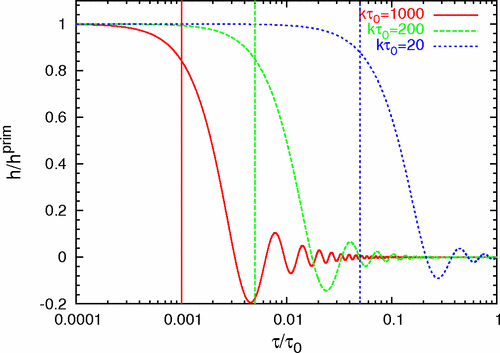
\includegraphics[width=0.7\linewidth, height=0.25\textheight]{Images/Chap3/Watanabe_Komatsu_Fig6}
	\caption{Numerical solutions of tensor perturbations. The solid, dashed, and short-dashed lines show the high, medium, and low frequency modes, respectively. The higher $k$-modes enter the horizon earlier, and are damped more by the cosmological redshift. Vertical lines define the horizon crossing time for each $ k $-mode\cite{Chap3:GW_Watanabe_Komatsu}.}
	\label{fig:watanabekomatsufig6}
\end{figure}

\begin{figure}
	\centering
	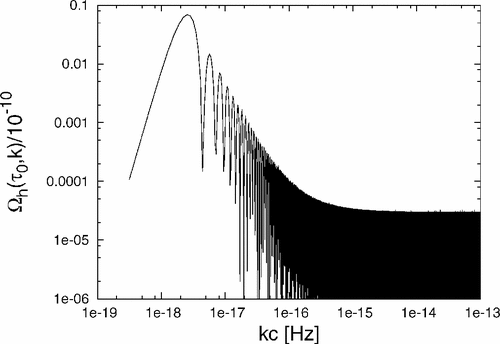
\includegraphics[width=0.7\linewidth, height=0.25\textheight]{Images/Chap3/Watanabe_Komatsu_Fig1}
	\caption{The primordial gravitational wave spectrum at present, $\tau=\tau_{0}$, as a function of the comoving number $ k $. The frequency of the gravitational waves observed today is related to $ k $ by $ f_{0}=kc/2\pi $. In the plot is assumed de-Sitter inflation and then the spectrum at large wavenumber is exactly scale-invariant. In this figure is not taken into account the effects of the change in relativistic degree of freedom or neutrino free-streaming \cite{Chap3:GW_Watanabe_Komatsu}.}
	\label{fig:watanabekomatsufig1}
\end{figure}

In (Fig. \ref{fig:watanabekomatsufig6}, \ref{fig:watanabekomatsufig1}) we report the plots in \cite{Chap3:GW_Watanabe_Komatsu} of the  numerical solutions for the temporal evolution of the GW modes and the primordial gravitational wave spectrum at present, respectevely.

The first solution (\ref{Chap3:Omega1}) describes $ \Omega_{GW}(\tau,k) $ during radiation era for the modes that entered the horizon before the time at the matter-radiation equality $ \tau_{eq} $. This solution is not relevant for what we observe today. The second (\ref{Chap3:Omega2}) and the third (\ref{Chap3:Omega3}) solutions describe $\Omega_{GW}(\tau,k)$ during matter era for the modes that entered the horizon before and after $\tau_{eq}$, respectively. While the expression is slightly complicated, one can find that the second solution is independent of k when the oscillatory part is averaged out, which explains  a scale-invariant spectrum at high frequencies, $ k>k_{eq} \sim 10^{-15} Hz $. On the other hand, the third solution gives $ \Omega_{GW}(\tau,k) \propto k^{-2} $.

These arguments can be understood in a more qualitative way and clearly seen in (Fig. \ref{fig:watanabekomatsufig1}). Energy density of gravitational waves evolves just like that of radiation inside the horizon, $ \tilde{\rho_{h}}(\tau,k) \propto a^{-4} $, for $ k\gg aH $. This implies that the relative spectral energy density, $ \Omega_{GW}(\tau,k) $, inside the horizon remains independent of time during the radiation era, while it decreases as $ \Omega_{GW}(\tau,k) \propto a^{-1} $ during the matter era. Thus, the modes that entered the horizon during the matter era \textit{later} would decay \textit{less}. As the low frequency modes represent the modes that entered the horizon at late times, $\Omega_{GW}(\tau,k)$ rises toward lower frequencies. On the other hand,  $\Omega_{GW}(\tau,k)$ at $  k > 10^{-15} $ is independent of k. These are the modes that entered the horizon  during the radiation era, for which $ \Omega_{GW} (\tau,k) $ was independent of time. After the matter-radiation equality all of these modes suffered the same amount of redshift, and then the shape of $\Omega_{GW}(\tau,k)$ still remains scale invariant at  $  k > 10^{-15} $.
\section{Thermal History}
In general it is granted that energy density of the universe evolves as $ \rho \propto a^{-4} $ during the radiation era, and this is exactly what caused a scale-invariant spectrum of $ \Omega_{GW}(k) $ at $ k > k_{eq}  $. However, $\rho \propto a^{-4}$ does not always hold in the radiation era because some particles would become non-relativistic before the others and don't contribute anymore to the radiation energy density. Since during the radiation era many kinds of particles interact with photons frequently, we can consider thermal equilibrium.

We recall that the energy density and the pressure in such era are given by 
\begin{equation}
\label{Chap3:EnergyDensityPressure}
 \rho(T)= \frac{\pi^{2}}{30}g_{*}T^{4} ,  
 \qquad
 p(T)=\frac{1}{3}\rho(T).
\end{equation}	
Moreover, we rewrite the expression for the entropy density,
\begin{equation}
	\label{Chap3:entropy}
	s(T)=\frac{2\pi^{2}}{45}g_{*s}(T)T^{3},
\end{equation}
with $ s(T) =(\rho(T) + p(T))/T $. The effective number of degrees of freedom, $ g_{*} $ and $ g_{*s} $, count respectively the (effective) number of relativistic species contributing to the radiation energy density and entropy. In an adiabatic system the entropy per unit comoving volume must be conserved, i.e. 
\begin{equation}
	\label{Chap3:conservationEntropy}
	S(T) = s(T)a^{3}(T) = constant.
\end{equation}
From the equation for energy density in (\ref{Chap3:EnergyDensityPressure}) we obtain the relation for the temperature
\begin{equation}
\label{Chap3:DependenceTemperature}
T = (30/\pi)^{1/4} \rho^{1/4}g_{*}^{-1/4} ,
\end{equation}
and, using (\ref{Chap3:conservationEntropy}),
\begin{equation}
	S(T)=\frac{2\pi^{2}}{45}g_{*s}(T)T^{3}a^{3} = \Big (\frac{2\pi^{2}}{45}\Big)\Big(\frac{30}{\pi}\Big)^{3/4} g_{*s}\ \rho^{3/4}g_{*}^{-3/4}a^{3} = const,
\end{equation}
from which we obtain the beheaviour of the energy density
\begin{equation}
	\label{Chap3:DependenceEnergyDensity}
	\rho \sim g_{*}g_{*s}^{-4/3}a^{-4}.
\end{equation}
We see then, unless $ g_{*} $ and $ g_{*s} $ are independent of time, the evolution of $\rho$ would deviate from $\rho \sim a^{-4}$. In other words, the evolution of $\rho$ during the radiation era is sensitive to how many relativistic species the universe had at a given epoch (Fig. \ref{fig:watanabekomatsufig2}).

\begin{figure}
	\centering
	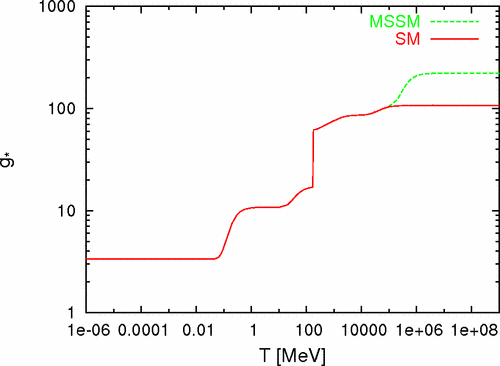
\includegraphics[width=0.7\linewidth, height=0.25\textheight]{Images/Chap3/Watanabe_Komatsu_Fig2}
	\caption{Evolution of the effective number of relativistic degree of freedom contribuiting to energy density, $ g_{*} $, as a function of temperature. The solid and dashed lines represent  $ g_{*} $ in the Standard Model and in the minimal extension of Standard Model (MSSM), respectively. MSSM also includes particles in supersymmetric models. At the energy scales above $ \sim 1$ TeV, $ g_{*}^{SM}=106.75 $ and $ g_{*}^{MSSM} \simeq 220 $. At energy scales below $ \sim 0.1 $ MeV, $ g_{*}\simeq 3.3626 $ and $ g_{*s}=3.9091 $; $ g_{*}=g_{*s} $ otherwise \cite{Chap3:GW_Watanabe_Komatsu}. }
	\label{fig:watanabekomatsufig2}
\end{figure}

We can then understand how $ g_{*} $ and $ g_{*s} $ would affect the shape of $ \Omega_{GW}(\tau_{0},k) $. While energy density of the universe  during the radiation era is affected by $ g_{*} $, $ g_{*s} $ as $ \rho_{cr} \propto g_{*}g_{*s}^{-4/3}a^{-4} $, energy density of  gravitational waves always evolves as $\tilde{\rho_{h}}(\tau,k) \propto a^{-4}$ inside the horizon, $ k \ll aH $, regardless $ g_{*} $ or $ g_{*s} $, because the gravitons are not in thermal equilibrium with other particles. Thus, this difference in the evolution of $ \tilde{\rho_{h}} $ and $ \rho_{cr} $ significantly modifies the spectrum of $ \Omega_{GW}(\tau_{0},k) $ at $ k>k_{eq} $.

Consider  a gravitational wave mode with $ k $ which entered the horizon at a given time $ \tau_{hc} < \tau_{eq} $ and temperature $ T=T_{hc} $ during the radiation era. After the mode entered the horizon its amplitude would be suppressed by the cosmological redshift. We can then derive, at first approximation, the relative spectral density $\Omega_{GW}(\tau_{0},k > k_{eq}) = \tilde{\rho_{h}}(\tau_{0},k)/\rho_{cr}(\tau_{0})$ today. Since energy density of gravitational waves is independent of other particles, we can write (the mode $ k $ entered the horizon during the radiation era at $ \tau_{hc} $)
\begin{equation}
 \tilde{\rho_{h}}(\tau_{0},k) =  \tilde{\rho_{h}}(\tau_{hc},k)\Big (\frac{a_{0}}{a_{eq}}\Big)^{-4}\Big (\frac{a_{eq}}{a_{hc}}\Big)^{-4},
\end{equation}
where the subscripts 0 and \textit{eq} denote the present value and the value at the radiation-matter equality, respectively.
Instead, the critical energy density of the universe during the matter era scales as $\sim a^{-3}$, and $ \sim g_{*}g_{*s}^{-4/3}a^{-4} $ during  the radiation era:
\begin{equation}
	\label{Chap3:CriticalDensityEvolution1}
	\rho_{crit}(\tau_{0})=\rho_{crit}(\tau_{eq})\Big(\frac{a_{0}}{a_{eq}}\Big)^{-3},
	\qquad
	\rho_{crit}(\tau_{eq})= \rho_{crit}(\tau_{hc})\Big[\frac{g_{*,0}}{g_{*}(T_{hc})}\Big]\Big [\frac{g_{*s,0}}{g_{*s}(T_{hc})}\Big]^{-4/3}\Big(\frac{a_{eq}}{a_{hc}}\Big)^{-4}.
\end{equation}  
Combining these equations in the expression for the relative spectral density of the GW at present, we obtain
\begin{equation}
	\label{Chap3:SpectralDensityAtPresent}
	\Omega_{GW}(\tau_{0}, k>k_{eq}) = \Omega_{GW}(\tau_{hc},k)\Big[\frac{g_{*s}(T_{hc})}{g_{*s0}}\Big]^{-4/3}\Big [\frac{g_{*}(T_{hc})}{g_{*0}}\Big] (1+z_{eq})^{-1},
\end{equation}
where we have used $ (1+z_{eq})^{-1} = a_{eq}/a_{0} $, with $ z_{eq}=3402 $. This equation helps us to understand how $ g_{*s} $ and $g_{*}$ would affect the beheaviour of $ \Omega_{GW}(\tau_{0},h) $.

The modes that entered the horizon earlier experienced larger suppression, as $ g_{*} $ and $ g_{*s} $ would be larger than the modes that entered the horizon later. The modes that entered the horizon during the matter era should not be affected by $ g_{*} $ or $ g_{*s} $, as they do not change during this era. (\ref{Chap3:SpectralDensityAtPresent}) can be obtained analytically also  directly from  the equation for the gravitational waves (\ref{Chap3:eomMasslessDesitter}), exploiting $ a''/a $ during the thermal history of the universe (see \cite{Chap3:GW_Watanabe_Komatsu}). 
In \cite{Chap3:GW_Watanabe_Komatsu} is also reported the full  computation of $ \Omega_{GW}(\tau_{0},k) $ obtained numerically integrating the wave equation together with the numerical data of $ g_{*} $ and $ g_{*s} $. The computation accounts also the effect of free-streaming of relativistic neutrinos which have decoupled from thermal equilibrium at $T < 2 $ Mev, and significantly contributes to damping the amplitude of the gravitational waves.

\begin{figure}
	\centering
	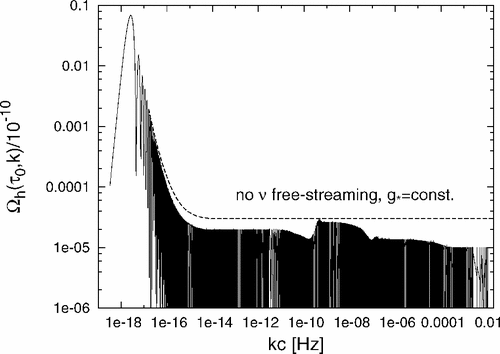
\includegraphics[width=0.7\linewidth, height=0.25\textheight]{Images/Chap3/Watanabe_Komatsu_Fig4}
	\caption{The primordial gravitational wave spectrum at present, $\Omega_{h}(\tau_{0},k)/10^{-10}$, as a function of the comoving wavenumber, $ k $. It is assumed a scale-invariant spectrum and $\Omega_{m}=1-\Omega_{r}, \Omega_{r} = 4.15 \times 10^{-5} h^{-2}, h=0.7$, and $ E_{inf}=10^{16} $ GeV. It is also included the effects of the effective number of relativistic degree of freedom and neutrino free-streaming. The dashed line shows the case in which these effects are ignored \cite{Chap3:GW_Watanabe_Komatsu}.}
	\label{fig:watanabekomatsufig4}
\end{figure}
The effect of the evolution of $ g_{*} $ and $ g_{*s} $ can be very important. For example, big changes in  $ g_{*} $ would occur at the electron-positron annihilation epoch ($\sim 0.51$ Mev, $\sim 2 \times 10^{-11}$ Hz), as well as the quark-gluon plasma (QGP) to hadron gas phase  ($\sim 180$ Mev, $\sim 10^{-7}$ Hz). From the analysis comes out that the gravitational wave spectrum is suppressed by roughly $ 20\% $ and $ 30\% $ above the electron-positron annihilation and QGP transition scales, respectively \cite{Chap3:GW_Watanabe_Komatsu}.

One may approximately relate the horizon crossing temperature of the universe to the frequency of the gravitational waves.  The horizon crossing mode, $ k_{hc} = a_{hc}H_{hc} $, is related to the temperature at that time by $ H^{2}_{hc}=\frac{8\pi G}{3}\rho_{hc}=\frac{8\pi^{3}G}{90}g_{*,hc}T^{4}_{hc} $. Using entropy conservation $ g_{*s,hc}a^{3}_{hc}T^{3}_{hc} = g_{*s0}a_{0}^{3}T_{0}^{3} $, one can obtain the following conversion factor  from the temperature of the universe to the frequency of gravitational waves observed today \cite{Chap3:Kamionkowsy_Turner},
\begin{equation}
		\label{Chap3:frequencyTodayGW}
		f_{0} = 1.65 \times 2\pi \times 10^{-7} \Big(\frac{T_{hc}}{1 Gev}\Big) \Big [\frac{g_{*s}(T_{hc})}{100}\Big]^{-1/3}  \Big [\frac{g_{*}(T_{hc})}{100}\Big]^{1/2} Hz ,
\end{equation}
 which is related to the comoving wavenumber, $ k $ (or $ kc $ in units of Hertz),  by $ 2\pi f_{0} = kc/a_{0} $.
 
 In an extremely high frequency region the gravitational wave spectrum should provide us unique informations about the reheating of the universe after inflation. On the other hand, in an extremely low frequency region (below $ \sim 10^{-18}$ Hz ) dark energy dominates the universe and affects the spectrum. The signatures of the primordial gravitational waves may be detected  by CMB polarization experiments in the low frequency region, $ < 10^{-16} $ Hz. For the higher frequency region, however, direct detection of the gravitational waves would be necessary, and it should allows us to search for a particular cosmological event, such as reheating.
\section{GW and Reheating}
In the previous section we have seen that the spectrum of the inflationary gravitational wave background directly reflects the expansion history of the universe. In particular, we see now that from  the direct detection of  gravitational waves we can extract informations about the reheating epoch, in particular the reheating temperature and the equation of state of the universe after inflation. 

As discussed, the growing mode solutions to the wave equation (\ref{Chap3:equationGWConformalTime}) have simple qualitative beheaviour: before the mode re-enters the horizon $ h_{\textbf{k}}(\tau) $ is constant. Once the modes cross inside the horizon during the radiation-dominated era the solution is $ h_{\textbf{k}}=h_{prim,\textbf{k}}(j_{0}(k\tau)) $, while for the modes that cross inside the horizon during the matter-dominated era the exact solution is $  h_{\textbf{k}}=h_{prim,\textbf{k}}(3j_{1}(k\tau)/k\tau) $. The Bessel function are given by $ j_{0}(x) = \sin x/x $ and $ j_{1}(x)= \sin x/x^{2} - \cos x/x $.

However, well into the matter dominated era the temporal beheaviour of modes that entered the horizon during the radiation-dominated era is also given by $(3j_{1}(k\tau)/k\tau)$.  For example, considering a gravitational wave mode of inflation that re-enters the horizon during the radiation era, its beheaviour is given by
\begin{equation}
\label{Chap3:GWSimpleBeheaviour}
h_{\textbf{k}}(\tau)=h_{\textbf{k}}^{prim}T(k/k_{EQ})\Big (\frac{3j_{1}(k\tau)}{k\tau}\Big),
\end{equation} 
where the transfer function of gravitational wave, $ T(k/k_{EQ}) $, is only a function of $ k/k_{EQ} $, with $ k_{EQ} \equiv a(t_{eq})H (t_{eq}) = 7.1 \times 10^{-2}\Omega_{m}h^{2} $ $ Mpc^{-1} $ \cite{Chap3:GW_Turner_White}.

The transfer function has been calculated by integrating (\ref{Chap3:equationGWConformalTime}) numerically from $ \tau=0 $ to $ \tau=\tau_{0} $ and we report the fit in (\ref{TransferFunction}) of \cite{Chap3:GW_Turner_White}, where this approach is introduced. 

However, as said in the previous section, the effect of the change of the relativistic degrees of freedom could be important. Indeed, during the expansion of the universe $ g_{*} $ changes and the expansion rate is modified from the simple power law $ a(t) \propto T^{-1} $ during radiation era. This effect yields the damping factor 
\begin{equation}
	\label{Chap3:dampingFactorDOF}
	\Bigg (\frac{g_{*}(T_{in})}{g_{*0}} \Bigg)\Bigg (\frac{g_{*s0}}{g_{*s}(T_{in})}\Bigg)^{4/3}
\end{equation}
on the power spectrum of the gravitational waves, where $ T_{in} $ denotes the temperature at which the corresponding mode enters the horizon, given by \cite{Chap3:ProibingReheatingTemperature2008}
\begin{equation}
	\label{T_{in}}
	T_{in} \simeq 5.8 \times 10^{6}\ Gev\ \Bigg (\frac{g_{*s}(T_{in})}{106.75}\Bigg)^{-1/6} \Bigg (\frac{k}{10^{14}Mpc^{-1}} \Bigg).
\end{equation}
Since we are interested about reheating, we consider the modes that re-enter the horizon during the reheating era. Moreover, we should also include the effect of dark energy that is leading today the expansion of the universe. 

 Before writing the solution we can rewrite the relative spectral density (\ref{Chap3:relativeSpectralDensity}) as
\begin{equation}
	\label{Chap3:RelativeSpectralDensity2}
	\Omega_{GW}(\tau,k) = \frac{\Delta_{T,prim}^{2}}{12H^{2}(\tau)a^{2}(\tau)}[T'(\tau,k)]^{2} = \frac{1}{12}\Bigg (\frac{k}{aH}\Bigg)^{2}\Delta_{h,prim}^{2}T^{2}_{h}(k).
\end{equation}
The last relation is a good approximation when we consider the modes deep inside the horizon, $ k \ll aH $. It is given by the fact  that the transfer function  is in general given by Bessel type functions, $ T(x) = \frac{1}{x^{n}}[Aj_{n}(x) + By_{n}(x)] $, and its conformal time derivative by $ T'(x) = -\frac{k}{x^{n}}[Aj_{n+1}(x) + By_{n+1}(x)] $, where $ x=k\tau $. Thus, in the limit $ k\ll aH $ we obtain (\ref{Chap3:RelativeSpectralDensity2}) \cite{Chap3:GW_Watanabe_Komatsu}.

In a single-field slow-roll inflation model the tensor-to-scalar ratio $ r = \Delta_{h,prim}^{2}(k_{0})/\Delta_{\zeta,prim}^{2}(k_{0}) $ can be related to the tilt of the tensor mode spectrum $ n_{T} = d \ln \Delta_{h,prim}^{2}(k_{0})/d \ln k  $ with $ r=-8n_{T} $. From $ r= - 8n_{T} $ we obtain the relation
\begin{equation}
	\label{Chap3:consistencyRelation}
	n_{T}=\frac{d \ln \Delta_{h,prim}^{2}(k)}{d \ln k} = -\frac{r}{8},
\end{equation}
from which
\begin{equation}
	\label{Chap3:ConsistencyRelation2}
	\frac{\Delta_{h,prim}^{2}(k)}{\Delta^{2}_{h,prim}(k_{0})} = \frac{k}{k_{0}}e^{-r/8},
\end{equation}
where $ k_{0} = 0.002 $ Mpc$^{-1}$ is the pivot scale. Thus, we can obtain from the expression of the tensor-to-scalar ratio $ r $ the equation \cite{Chap3:ProspectsForDeterminationWithDetectors}
\begin{equation}
	\label{Chapter3:solutionSpectrumDelta}
	\Delta^{2}_{h,prim}(k) \simeq r\Delta_{\zeta,prim}^{2}(k_{0})\ \exp \Bigg[-\frac{r}{8}\ln \frac{k}{k_{0}} + ... \Bigg].
\end{equation}
The effects of the cosmological evolution after inflation are then all included in the transfer function $ T_{h}(k) $ in (\ref{Chap3:relativeSpectralDensity}) \cite{Chap3:ProspectsForDeterminationWithDetectors}:
\begin{equation}
	\label{Chap3:FinalTransferFunction}
	T^{2}_{h}(k) = \Omega_{m}^{2}\Bigg (\frac{g_{*}(T_{in})}{g_{*0}}\Bigg)\Bigg (\frac{g_{*s}(T_{in})}{g_{*s0}}\Bigg)^{-4/3} \Bigg ( \overline{\frac{3j_{1}(k\tau_{0})}{k\tau_{0}}}\Bigg)^{2} T_{1}^{2}(x_{eq})T^{2}_{2}(x_{R}).
\end{equation}
The subscript 0 denotes the present time, and the subscript \textit{in} denotes the time when the mode crosses the horizon. The effective number of degrees of freedom at the end of reheating is taken to be the sum of the standard model particles,  $ g_{*}(T_{R}) $ =  $ g_{*s}(T_{R}) = 106.75 $. The values at present are $ g_{*0}=3.36 $ and $ g_{*s0}=3.90 $. $\tau_{0}$ is the present conformal time calculated assuming the universe matter dominated, $ \tau_{0}=2H_{0}^{-1} $. The parameter $\Omega_{m}=\-\Omega_{\Lambda}  $ accounts for the effect of the cosmological constant. In the limit of $ k\tau_{0} \ll 1 $ the spherical Bessel function $ j_{1}(x)=(\sin x -  x\cos x)/x^{2} $ is replaced by $ \overline{j_{1}(k\tau_{0})} \simeq \overline{\cos (k\tau_{0})}/(k\tau_{0}) = 1/(\sqrt{2}k\tau_{0}) $. The first transfer function $ T_{1}(x_{eq}) $  describes the change of the frequency dependence of the spectrum which arises from the change of the expansion rate of the universe at the matter-radiation equality $ t=t_{eq} $
\begin{equation}
	\label{TransferFunction}
	T_{1}^{2}(x_{eq})=[1+1.57 x_{eq} + 3.42 x_{eq}^{2} ],
\end{equation}
where $ x_{eq} = k/k_{eq} $ and $ k_{eq} \equiv \tau_{eq}^{-1} = 7.1 \times 10^{-2} \Omega_{m} h^{2} $ Mpc$^{-1}$. The second transfer function $ T_{2}(x_{R}) $ corresponds to the change of the expansion rate at the end of reheating $ t=t_{R} $ and connects the modes which enter the horizon after and before  reheating ends. 

Since before the inflaton decays the universe was dominated by the coherent oscillation of the inflaton, the spectrum of the gravitational waves changes for the modes which enter the horizon at the inflaton dominated epoch $ (k>k_{R}) $, where
\begin{equation}
	\label{Chap3:kReheating}
	k_{R}\simeq 1.7 \times 10^{13} Mpc^{-1} \Bigg(\frac{g_{*}(T_{R})}{106.75}\Bigg)^{1/6}\Bigg(\frac{T_{R}}{10^{6}Gev}\Bigg).
\end{equation}
In terms of frequency, this corresponds to 
\begin{equation}
	\label{Chap3:frequencyReheating}
	f_{R} \simeq 0.026\ Hz \Bigg (\frac{g_{*s}(T_{R})}{106.75}\Bigg)^{1/6}\Bigg ( \frac{T_{R}}{10^{6} Gev} \Bigg),
\end{equation}
which is close to the most sensitive frequency of detectors like DECIGO \cite{Chap3:ProibingReheatingTemperature2008}. The transfer function $ T_{2}(x_{R}) $ is obtained  by solving simultaneously the gravitational waves equation and the Friedmann equations taking into account the decay of the inflaton,
\begin{equation}
\ddot{h}_{\lambda,k} + 3H\dot{h}_{\lambda,k} + \frac{k^{2}}{a^{2}}h_{\lambda,k} = 0,
\end{equation}
\begin{equation}
	\dot{\rho_{\phi}} + 3H\rho_{\phi} = -\Gamma_{\phi}\rho_{\phi},
\end{equation}
\begin{equation}
	\dot{\rho_{r}} + 4H\rho_{r} = \Gamma_{\phi}\rho_{\phi},	
\end{equation}
\begin{equation}
	H^{2}=\dfrac{8\pi G}{3}(\rho_{\phi} + \rho_{r}),
\end{equation}
where $\rho_{\phi}$ denotes the energy density of the inflaton coherent oscillation. The best fit of $ T_{2}(x_{R}) $ is given by \cite{Chap3:ProibingReheatingTemperature2008}:
\begin{equation}
	\label{Chap3:TransferFunction2}
	 T_{2}^{2}(x_{R}) = [1-0.32 x_{R} + 0.99 x^{2}_{R}]^{-1},
\end{equation}
where $ x_{R} = k/k_{R} $.

$\Omega_{GW}(f)$ beheaves  as $ f^{0} $ for modes which enter the horizon in the radiation era, while it beheaves as $ f^{-2} $ for  modes which enter in the matter era (see later). Since the evolution of inflationary gravitational waves is sensitive to the expansion of the universe, $ H^{-1} $, we obtain a characteristic feature for the modes around $ f \sim f_{R} $. If the universe beheaves like a matter-dominated universe during reheating, the transition from reheating to the radiation domination era is seen as a change of the frequency dependence of the spectrum. If this signature exists in the frequency band of direct detection sensitivity, $ 0.1-1 $ Hz, we may able to determine the reheating temperature by measuring the knee-like feature where the frequency dependence changes from $ f^{-2} $ to $ f^{0} $. In this view, $ f_{R} $ is the important frequency where the change of the frequency dependence due to reheating arises. We show the spectra for different values of the reheating temperature in (Fig. \ref{fig:kurojanaginakayamafig1}) from \cite{Chap3:ProspectsForDeterminationWithDetectors}, where we can see the knee shape around $ f_{R} $.

\begin{figure}
	\centering
	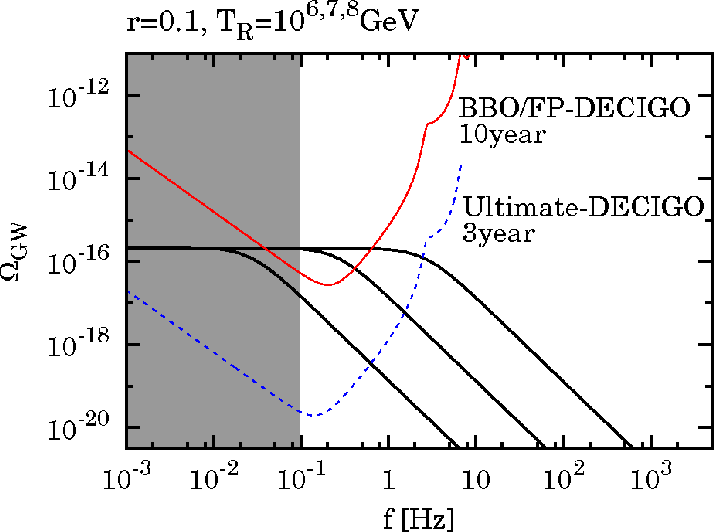
\includegraphics[width=0.7\linewidth, height=0.3\textheight]{Images/Chap3/Kurojanagi_Nakayama_Fig1}
	\caption{The spectra of the inflationary gravitational wave background for different values of the reheating temperature (thick black solid curves with $ T_{R}=10^{6},10^{7},10^{8} $ GeV from left to right). The tensor-to-scalar ratio is taken to be $ r=0.1 $. For reference, it is also plotted the noise spectra for BBO/FP-DECIGO with 10-year observation (red solid) and for Ultimate-DECIGO with 3-year observation (blue-dotted).  The grey  shaded region represents where the noise coming from white dwarf binaries may significantly contribute as systematic error \cite{Chap3:ProspectsForDeterminationWithDetectors}.}
	\label{fig:kurojanaginakayamafig1}
\end{figure}
\begin{figure}
	\centering
	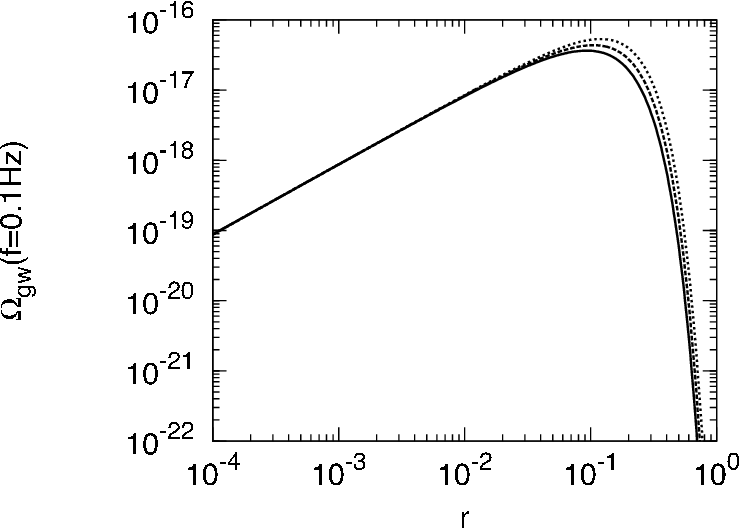
\includegraphics[width=0.7\linewidth, height=0.3\textheight]{Images/Chap3/Nakayama_Saito_Fig2}
	\caption{The spectrum $\Omega_{GW}(f)$ at $ f=0.1 $ Hz for $ \eta=0.01,0,-0.01 $ from upper to lower \cite{Chap3:ProibingReheatingTemperature2008}}.
	\label{fig:nakayamasaitofig2}
\end{figure}
\begin{figure}
	\centering
	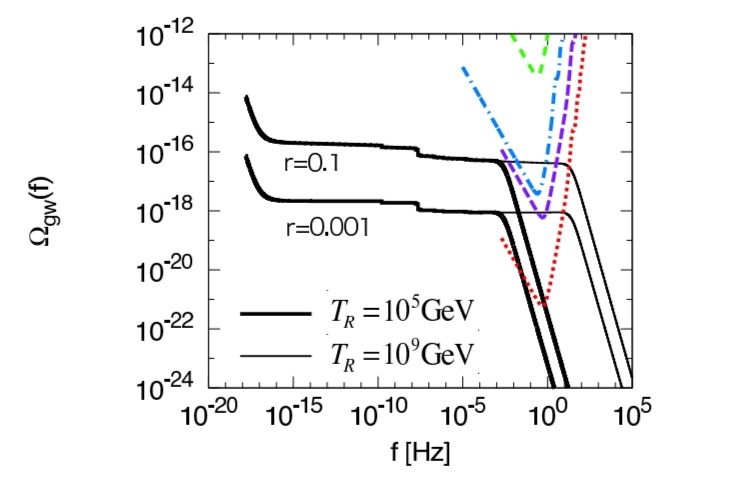
\includegraphics[width=0.8\linewidth, height=0.3\textheight]{Images/Chap3/Nakayama_Saito_FirstPlot}
	\caption{Primordial gravitational wave spectrum for $ T_{R}=10^{9}$ GeV and $ T_{R}=10^{5}$ GeV are shown by thin and thick lines for $ r=0.1 $ and $ r=0.01 $. Also shown are expected sensitivity of DECIGO (green dashed), correlated analysis of DECIGO (blue-dot dashed), Ultimate-DECIGO (purple dashed) and correlated analysis of ultimate-DECIGO (red dotted), from upper to lower \cite{Chap3:ProibingReheatingTemperature2008}. }
	\label{fig:nakayamasaitofig3}
\end{figure}
We also report in (Fig. \ref{fig:nakayamasaitofig2}) and (Fig. \ref{fig:nakayamasaitofig3})   two plots from \cite{Chap3:ProibingReheatingTemperature2008}. The first plot shows the resulting spectrum $\Omega_{GW}(f)$ at $ f=0.1 $ Hz for the values of the slow-roll parameter $\eta = 0.01, 0, -0.01$  from upper to lower (it is assumed $ T_{R} \le  10^{9}$). The second plot shows the resulting gravitational wave spectrum for $ T_{R}=10^{9} $ GeV and $ 10^{5} $ GeV with $ r=0.1 $ and $ r=0.001 $. 

Thus, the spectrum of the primordial gravitational wave background generated during inflation crucially depends on the reheating temperature $ T_{R} $.  This fact opens the possibility that future experiments devoted to detect the gravitational wave background will probe the reheating stage of the universe.

The important parameters that determine the primordial gravitational wave spectrum are the tensor-to-scalar ratio $ r $ and the reheating temperature $ T_{R} $. The tensor-to-scalar ratio $ r $ determines the overall normalitation of the spectrum (the amplitude), and $ T_{R} $ fixes the frequency above which the spectrum is significantly suppressed. The important point is that if the knee point in the spectrum  determined by $ T_{R} $ around the frequency $ f_{R} $ lies above the sensitivity of future detectors, $ T_{R} $ can be determined by observation of gravitational waves.

The non-zero value of the tensor-to-scalar ratio $ r $ is determined by measurements of the B-mode CMB polarization,  whose detection indirectly would confirm the existence of the primordial gravitational wave background. A certain amount of B-modes polarization has been detected  by BICEP2 collaboration, but the amplitude is compatible with foreground contamination. Current data actually provide only an upper bound on r ($ r_{0.05} < 0.09 $ at $ 95 \% $ C.L.).

In \cite{Chap3:ProibingReheatingTemperature2008} and \cite{Chap3:ProspectsForDeterminationWithDetectors} is studied the observable range of $ T_{R} $  for various value of $ r $, through future mission concepts based on space laser interferometers, like DECIGO \cite{Chap3: DECIGO} and NASA's Big Bang Observer (BBO). DECIGO is a future mission that will explore the gravitational wave range frequency $ 0.1 < f < 10 $ Hz, which would contains important informations about the primordial epoch and likely can put a meaningful constraint on $ T_{R} $. However, stochastic noise coming from some astrophysical sources must be taken into account for the purpose of detecting gravitational wave background. In particular, gravitational waves from white-dwarf binaries are considered to completely hide the primordial ones for the frequencies $ f<0.1 $ Hz. But for the frequency range $ 0.1-10 $ Hz, where DECIGO and BBO are most sensitive, foregrounds from astrophysical sources can be separated. 

From the analysis of \cite{Chap3:ProibingReheatingTemperature2008}, for $ 10^{-3} \le r \le 1 $, direct detection of the gravitational wave background can determine the reheating temperature $ T_{R} $ if it lies in the range $ T_{R} \sim 10^{6}-10^{8} $ Gev.

On the other hand, in \cite{Chap3:ProspectsForDeterminationWithDetectors} the detectability of $ T_{R} $ is studied using the Fisher information matrix approach. This Fisher matrix is a powerful method used in cosmology to forecast the constraining power of parameter of interest for a given survey.

The Fisher matrix  generally depends on the covariance matrix of signals, i.e. the noise properties of the survey configurations. In the case of the stochastic gravitational wave background direct detection can be attempted by cross-correlating the output signals between detectors. The Fisher matrix $ \mathcal{F}_{ij} $ depends on three ingredients: a total observational time $ T_{obs} $, an overlap reduction function $ \gamma_{ij}(f) $ and the noise spectra $ S_{I}(f) $. These functional forms rely on the type of interferometry that we choose. Both DECIGO and BBO are basically designed to aim at the detection of the inflationary gravitational waves with similar frequency ranges around $ 0.1-10 $ Hz. It is chosen a lower cutoff of $ f_{cut}=0.1  $ Hz, below which the signal may be contaminated by noise from cosmological white dwarf binaries. On the other hand, $ f_{max} $ is set to $ f_{max}=\infty $. 

The Fisher matrix is a product of the signal-to-noise ratios, $ \Omega_{GW}/S $, and the derivative, $ \partial_{p_{i}} \ln \Omega_{GW} $, and hence depends on the parameter response, namely the parameter degeneracy as well as the signal detectability. Fisher matrix can be calculated once the detector parameters are assigned and theoretical predictions for $\Omega_{GW}$ is provided.

The marginalized $ 1\sigma $ error is computed with the inverse of the Fisher matrix 
$ \sigma(p_{i}) = \sqrt{(\mathcal{F})^{-1}_{ii}} $. 
We can estimate the detectability of the reheating temperature substituing the expression of the relative spectral density (\ref{Chap3:spectralDensityFinal}) in the Fisher matrix, given by
\begin{equation}
	\label{FisherMatrix}
	\mathcal{F}_{ij}= \Bigg (\frac{3H_{0}^{2}}{10\pi^{2}}\Bigg)^{2}2T_{obs}\sum_{(I,J)}\int_{f_{cut}}^{f_{max}}
	df\frac{|\gamma_{ij}(f)|^{2} \partial_{p_{i}} \Omega_{GW}(f)\partial_{p_{j}}\Omega_{GW}(f)}{f^{6}S_{I}(f)S_{j}(f)}.
\end{equation}
The paramaters  $ r $ and $ T_{R} $ are taken as free and correspond to the amplitude of the spectrum and the frequency of the reheating signature, respectevely. In the plot (Fig. \ref{fig:kurojanaginakayamafig2}) from \cite{Chap3:ProspectsForDeterminationWithDetectors} is presented an example of future constraints. The fiducial parameters are chosen as $ r = 0.1 $ and $ T_{R}=10^{7} $ Gev. Each ellipse represents the $ 2\sigma $ error contours expected from 1, 3 and 10 years of observation with 	BBO/DECIGO. The error ellipse shrinks more for longer observations due to the fact that the signal-to-noise ratio scales as $\sqrt{T_{obs}}$. 

\begin{figure}
	\centering
	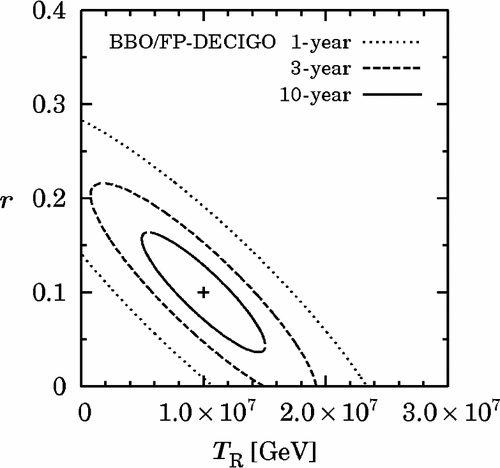
\includegraphics[width=0.7\linewidth, height=0.3\textheight]{Images/Chap3/Kurojanagi_Nakayama_Fig2}
	\caption{The $ 2\sigma $ confidence level contours in the $ T_{R}-r $ plane for 1-year (dotted), 3-year (dashed) and 10-year (solid) observation by BBO/FP-DECIGO. The fiducial parameters are set as $r=0.1$ and $ T_{R}=10^{7} $ GeV, which is shown by a cross mark \cite{Chap3:ProspectsForDeterminationWithDetectors}. }
	\label{fig:kurojanaginakayamafig2}
\end{figure}
\begin{figure}
	\centering
	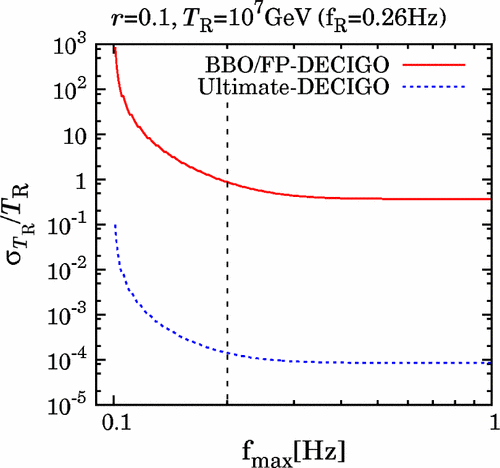
\includegraphics[width=0.7\linewidth, height=0.3\textheight]{Images/Chap3/Kurojanagi_Nakayama_Fig3}
	\caption{The $ 1\sigma $ margnalized errors are shown as a function of $ f_{max} $, calculated assuming $ r=0.1 $ and $ T_{R}=10^{7} $ GeV (corresponding to $ f_{R}=0.26 $ Hz) with 3-year observations. The best sensitivity frequency is plotted as a vertical line \cite{Chap3:ProspectsForDeterminationWithDetectors}.}
	\label{fig:kurojanaginakayamafig3}
\end{figure}
Another interesting question examinated in \cite{Chap3:ProspectsForDeterminationWithDetectors} is what frequency range actually carries information about the reheating temperature, i.e. how wide of a band  width is necessary to detect the knee shape with a good accuracy. We report the plot of \cite{Chap3:ProspectsForDeterminationWithDetectors} in (Fig. \ref{fig:kurojanaginakayamafig3}) in which errors in $ T_{R} $ are plotted as a function of the upper frequency limit in the calculation of the Fisher matrix ($ f_{max} $). From the analysis in the paper, apparently frequencies above $ f \simeq 0.3$ Hz do not contribute to detection of the reheating temperature. This is because both the suppression of the signal amplitude due to reheating and the increase of the noise spectrum intensity prevents us from reaching the spectrum informations.

Instead of choosing fixed values of $ r $ and $ T_{R} $, we can discuss the fiducial dependence and predict the parameter space where the signature of reheating can be successfully detected. In (Fig. \ref{fig:kurojanaginakayamafig4}) from \cite{Chap3:ProspectsForDeterminationWithDetectors} the marginalized error in $ T_{R}(\sigma_{T_{R}})$							
is calculated by changing $ r $ with the fixed value of $ T_{R}=10^{7} $ Gev. The error becomes smaller as the gravitational wave spectrum is detected with larger signal-to-noise ratio (the spike in the figure is an artificial effect due to the choice of parametrization). Similarly in (Fig. \ref{fig:kurojanaginakayamafig5}) from \cite{Chap3:ProspectsForDeterminationWithDetectors} is shown the dependence on the fiducial value of $ T_{R} $ with the fixed value of $ r = 0.1 $. From the plot we can see that the error becomes smaller when the signature of reheating comes into the range of the sensitivity, which corresponds to the reheating temperature of about $ 10^{6} $ Gev to $ 10^{8} $ Gev. The right panel of (Fig. \ref{fig:kurojanaginakayamafig5}) shows that Ultimate-DECIGO could determine the reheating temperature with $ 1 \% $ accuracy of $ 1.2 \times 10^{6} $ Gev $ < T_{R} <  3.3 \times 10^{8} $ Gev for $ r=0.1 $, and if $ 2.1 \times 10^{6} $ Gev  $ < T_{R} < 7 \times 10^{7} $ Gev, for $ r=0.01 $. We also report in (Fig. \ref{fig:kurojanaginakayamafig6}) from \cite{Chap3:ProspectsForDeterminationWithDetectors}  the parameter space of $ r $ and $ T_{R} $, where the reheating signature is detected at greater than $ 2\sigma $ level ($ T_{R} / \sigma_{T_{R}}  > 2$)  with 3-year observation. It is also shown the parameter region for the detection with a signal-to-noise ratio higher than 5 ($ S/N > 5 $), that is the criterion adopted in \cite{Chap3:ProibingReheatingTemperature2008}. However, in \cite{Chap3:ProibingReheatingTemperature2008} is not taken into account the degeneracy between the parameters $ T_{R} $ and $ r $, given by the fact that as long as the frequency dependence of the spectrum is measured with a good accuracy, we cannot distinguish the spectrum with larger $ T_{R} $ from that with smaller amplitude, i.e. with smaller $ r $. This may cause an underestimate of $ \sigma_{T_{R}} $.
\begin{figure}[]
	\centering
	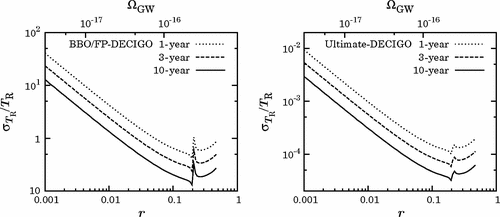
\includegraphics[width=0.8\linewidth, height=0.25\textheight]{Images/Chap3/Kurojanagi_Nakayama_Fig4}
	\caption{The marginalized $ 1\sigma $ uncertainty in $ T_{R} $ as a function $ r $ of BBO/DECIGO (left panel) and Ultimate-DECIGO (right panel). The fiducial value of the reheating temperature is fixed to be $ T_{R}=10^{7} $ GeV. The upper horizontal axis represents the values of $ \Omega_{GW} $ corresponded to $ r $ by (\ref{Chap3:RelativeSpectralDensity2}) \cite{Chap3:ProspectsForDeterminationWithDetectors}. \label{fig:kurojanaginakayamafig4}}
\end{figure}
\begin{figure}[]
	\centering
	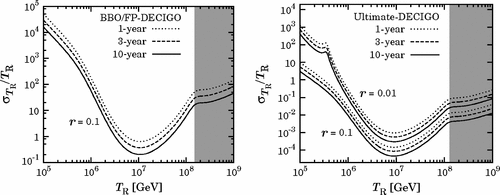
\includegraphics[width=0.8\linewidth, height=0.25\textheight]{Images/Chap3/Kurojanagi_Nakayama_Fig5}
	\caption{The marginalized $ 1\sigma $ uncertainty in $ T_{R} $ as a function of $ T_{R} $ for BBO/DECIGO (left panel) and Ultimate-DECIGO (right panel). The fiducial value of the tensor-to-scalar ratio is fixed to be $ r=0.1 $ \cite{Chap3:ProspectsForDeterminationWithDetectors}.}
	\label{fig:kurojanaginakayamafig5}
\end{figure}
\begin{figure}[]
	\centering
	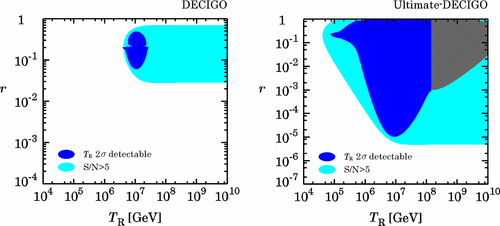
\includegraphics[width=0.8\linewidth, height=0.25\textheight]{Images/Chap3/Kurojanagi_Nakayama_Fig6}
	\caption{$ 2\sigma $ detection of $ T_{R} $ is shown as a blue shaded region for 3-years observations by BBO-FP-DECIGO (left panel) and Ultimate-DECIGO (right panel). The gray area represents the region where $ \sigma_{T_{R}} $ may be underestimated in the previous work \cite{Chap3:ProibingReheatingTemperature2008}, where the Fisher approach was not used. In the light blue shaded region  the inflationary gravitational wave background would be detected with a signal-to-noise ratio higher than 5 \cite{Chap3:ProspectsForDeterminationWithDetectors}.}
	\label{fig:kurojanaginakayamafig6}
\end{figure}
\section{Late-time Entropy Production}
So far we have assumed that there were no late-time entropy production processes after the completion of reheating after inflation. Let us consider also the case in which some other scalar field $\sigma$  dominates the universe some time after the inflaton decays. This new particle eventually decays releasing huge entropy. In some cases, during the radiation-dominated era after the decay of the inflaton, the oscillating $\sigma$ field can dominate over the radiation energy density. Then, the universe enters a matter-dominated like phase due to the $\sigma$ oscillation. After the $\sigma$-field decays into radiation the universe is dominated by the radiation energy again. Such a scenario can be interesting since it diluites all cosmological relics produced in the reheating era. 

This non-standard cosmological evolution is imprinted in the present gravitational wave spectrum. In the presence of such a late-decaying particle, the additional $\sigma$-matter dominated era suppresses the gravitational wave amplitude for the frequencies which re-entered the horizon during or before $\sigma$ begins to dominate the universe \cite{Chap3:ProibingReheatingTemperature2008}. The fitting formula for the transfer function is given by \cite{Chap3:ProibingReheatingTemperature2008}
\begin{equation}
	\label{Chap3:TransferFunctionLateEntropy}
	T^{2}_{h} = \Omega_{m}\Bigg(\frac{g_{*}(T_{in})}{g_{*0}}\Bigg)\Bigg(\frac{g_{*s0}}{g_{*s}(T_{in})}\Bigg)^{4/3}\Bigg (\frac{3j_{1}(k\tau_{0})}{k\tau_{0}}\Bigg)^{2}T_{1}^{2}(x_{eq})T_{2}^{2}(x_{\sigma})T_{3}^{2}(x_{\sigma R})T^{2}_{2}(x_{RF}),
\end{equation}
where $ k_{\sigma} $ corresponds to the wavenumber which enters the horizon at the time  when $\sigma$ decays into radiation after the $\sigma$-dominated era, and it is given by
\begin{equation}
\label{Chap3:kSigma}
k_{\sigma} = 1.7 \times 10^{14} \Bigg (\frac{g_{*s}(T_{\sigma})}{106.75}\Bigg)^{1/6}\Bigg (\frac{T_{\sigma}}{10^{7} Gev}\Bigg) Mpc^{-1},
\end{equation}
with $ T_{\sigma} $ being the temperature of the universe at the $\sigma$ decay. Before writing down $ k_{\sigma R} $ and $ k_{RF} $, we define the \textit{diluition factor} F, which represents the amount of entropy production by the decay of $\sigma$:
\begin{equation}
	\label{Chap3:DiluitionFactor}
	F \equiv \frac{s(T_{\sigma})a^{3}(T_{\sigma})}{s(T_{R})a^{3}(T_{R})},
\end{equation}
where $ s(T) $ is the entropy density at temperature T. The abundance of all dangerous cosmological relics produced in the reheating era after inflation are diluited by this factor.

With this quantity  we can define the other characteristic frequencies as $ k_{\sigma R}=k_{\sigma}F^{2/3} $ and $ k_{RF}=k_{R}F^{-1/3} $. The third transfer function $ T_{3}(x) $ describes the transition from the first radiation-dominated era to the $\sigma$-dominated phase and it is given by \cite{Chap3:ProibingReheatingTemperature2008}
\begin{equation}
	\label{Chap3:ThirdTransferFunction}
	T_{3}(x) = 1 + 0.59x + 0.65x^{2}.
\end{equation}
For the modes $ k_{\sigma R} < k < k_{R}$, which correspond to the modes which re-enter the horizon in the radiation dominated era before the $\sigma$ domination, the energy density of the gravitational waves is suppressed by the factor $\sim (k_{R}/k_{\sigma R})^{2} = F^{-4/3}$ \cite{Chap3:Seto_Yokohama}. On the other hand, there are no effects on large scales with the modes $ k < k_{\sigma} $.

The gravitational wave spectrum in the presence of late-time entropy production is then completely characterized by two additional parameters: the diluition factor F and the decay temperature of $\sigma$, $ T_{\sigma} $. Non-negligible effects of $ F $ can affect the overall amplitude of the gravitational wave background for the modes $ k_{\sigma R} < k < k_{R} $, and hence there is a degeneracy between F and the tensor-to-scalar ratio $ r $ when we consider the direct detection around $ 0.1 $ Hz. However, $ r $ should be determined by CMB B-mode measurements. Thus, if future CMB experiments measure $ r $, there does not remain any ambiguity coming from the degeneracy between $ r $ and $ F $. This means that if the results of direct detection experiments deviate from the expected signal from the large scale measurements of $ r $, there must be an entropy production process in the early universe. In (Fig. \ref{fig:nakayamasaitofig6}) from \cite{Chap3:ProibingReheatingTemperature2008} is plotted the gravitational wave spectrum with $ F=10^{2} $ and $ F=10^{4} $, with $ r=0.1 $, $ T_{R}=10^{9} $  Gev and $ T_{\sigma} = 1 $ Gev. The figure shows how the gravitational wave spectrum is affected by late-time entropy production.

If $ 0.1$ Hz $ < k_{R}(F) <10$ Hz, both $ F $ and $ T_{R} $ can be determined from the shape of the gravitational wave spectrum. In the figure are shown also the future sensitivities to determine the diluition factor $ F $ and the reheating temperature $ T_{R} $ with fixed tensor-to-scalar ratio $ r $, which can be measured by CMB polarization experiments.
\begin{figure}
	\centering
	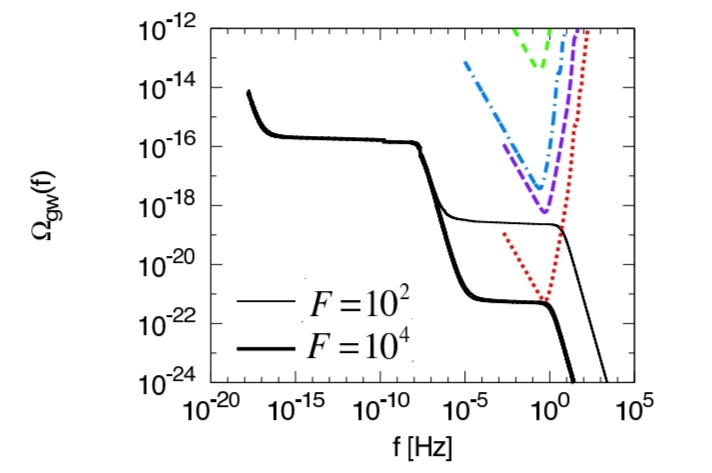
\includegraphics[width=0.8\linewidth, height=0.3\textheight]{Images/Chap3/Nakayama_Saito_SecondPlot}
	\caption{Gravitational wave spectrum for the diluition factor $ F=10^{2} $ and $ F=10^{4} $. Here is set $ r=0.1, T_{R}=10^{9} $ GeV and $ T_{\sigma}=1 $ GeV. Also shown are expected sensitivity of DECIGO (green dashed), correlated analysis of DECIGO (blue-dot dashed), Ultimate-DECIGO (purple dashed) and correlated analysis of ultimate-DECIGO (red dotted), from upper to lower \cite{Chap3:ProibingReheatingTemperature2008}.}
	\label{fig:nakayamasaitofig6}
\end{figure}

\section{Blue-tilted Spectrum}
Although the standard inflation model predicts a red-tilted spectrum since the tensor spectral index $ n_{T} $ has the so-called consistency relation $ n_{T}=-r/8 $, a blue-tilted spectrum can be realized in some non-standard models. There are several observational constraints on the energy density of the stochastic gravitational waves at different frequencies given by pulsar timing, Big-Bang Nucleosynthesis (BBN), interferometric GW detectors such as LIGO and VIRGO and so on. Although these limits are far above the predictions of the standard inflationary models, a strongly blue-tilted tensor spectrum can instead  be detected. Moreover, the mechanisms that generate GW do not necessary  predict a blue-tilted spectrum over all the frequencies. The spectral index of the primordial GW spectrum can change at some frequency. 

We can use two different approaches to describe GW spectrum. In the first approach we consider constraints on $ n_{T} $ taking into account the suppression of the spectrum at high frequencies due to reheating and late-entropy production, assuming that the primordial spectrum has uniform spectral index over all frequencies. Until now we used this approach considering a fitting formula that can reproduce the effect of the thermal history of the universe on the spectrum with a very good accuracy.

In the second approach, introduced in \cite{Chap3:BlueTiltedSpectrum},  we can consider the constraints on $ n_{T} $ without assuming an explicit model of the early universe. Since the shape of the GW spectrum strongly depends on the model assumed, in \cite{Chap3:BlueTiltedSpectrum}
a more general form of the spectrum  is used such that the spectral index changes from $ n_{T} $ to a different value at a given frequency. In this way, we can also include the case where the universe is dominated by a component whose equation of state differs from that of radiation/matter component.

We first summarize observational bounds on the energy density of the stochastic GW, which are used to obtain constraints on $ n_{T} $. The constraints adopted are the stringest ones from interferometric GW detectors, pulsar timing array, and BBN. For details and references for this section see \cite{Chap3:BlueTiltedSpectrum}. Here we discuss the main results of the paper.
\subsection*{LIGO + VIRGO}
From interferometric GW detectors, such as LIGO, we obtain an upper bound on the stochastic GW given  by the fact that we don't detect them until now. It is adopted $ 95\% $ C.L. upper bound from the LIGO-Virgo collaboration  \cite{Chap3:Ligo_Virgo}
\begin{equation}
	\label{Chap3:LigoVirgo}
	\Omega_{GW}h^{2} < 2.6 \times 10^{-6} \qquad  [f = 41.5 - 
	169.25\ Hz] ,
\end{equation}
where $ h $ is the dimensionless Hubble parameter that parametrizes the present Hubble constant as $ H_{0} = 100h\  km/s $. The analysis is performed using the approximate form of the GW spectrum, $ \Omega_{GW}(f)=\Omega_{GW,\alpha}(f/100Hz)^{\alpha}, $ where $\alpha$ is the local power index around the sensitive frequency $\sim 100$ Hz, where (\ref{Chap3:LigoVirgo}) is obtained assuming $\alpha=0$.
\subsection*{Pulsar timig array}
 The millisecond pulsars are very precise clocks. Gravitational waves can be searched through the effect of the pulse arrival timings, which currently provides the stringest constraint on the amplitude of GW at $ f\sim 10^{-8} $ Hz. We can use the bounds obtained by the North American Nanohertz Observatory for Gravitational waves (NANOGrav) project, which gives the upper bound \cite{Chap3:PulsarTiming}
 \begin{equation}
 	\Omega_{GW}h^{2} < 1.1 \times 10^{-8}   \qquad [f = 1/(5.54 years) = 5.72 \times 10^{-9} Hz],
 \end{equation}
where GW spectrum is modeled by $ h_{c}(f) = A_{1year}(f/f_{1year})^{\beta} $, which corresponds to $\Omega_{GW}(f)=(2\pi^{2}/3H_{0}^{2})f^{2}h_{c}^{2}(f)$, and $ A_{1year} $ is well approssimated by $ A_{1year}=2.26\times 10^{-14}(5.54year/1year)^{\beta}$.
\subsection*{BBN}
We can also consider contraints from Big-Bang nucleosynthesis. Primordial GW contribute to the energy density of the universe as an extra radiation component. Such extra radiation  changes the expansion rate of the universe during BBN and affects the abundance of the light elements. The total energy of GW, given by integrating the density  parameter  $ \Omega_{GW}(f) $, is therefore constrained not to spoil BBN:
\begin{equation}
	\label{Chap3:ConstraintsBBN}
	\int_{f_1}^{f_2} d(\ln f)\Omega_{GW}(f)h^{2} \le 5.6 \times 10^{-6}(N^{(upper)}_{eff} - 3),
\end{equation}
where $ N^{(upper)}_{eff} $ is the upper bound on the effective number of extra radiation at the time of BBN. The lower limit $ f_1 $ is given by the frequency  corresponding to the comoving horizon at the time of BBN, and $ f_{1}=10^{-10} $ Hz is taken. For the upper cutoff $ f_{2}=10^{7} $ Hz is taken, which corresponds to the temperature of the universe $ \sim 10^{15} $ Hz. In \cite{Chap3:BlueTiltedSpectrum} is adopted the $ 95 \% $ C.L. upper limit of $ N^{(upper)}_{eff} = 4.65 $.
\\

We illustrate how these observational bounds on $\Omega_{GW}(f)$ can provide upper bounds to $ n_{T} $ in consideration of  reheating and late-entropy production. Large values of $ n_{T} $ can elude the observational constraints if the reheating temperature is low or the amount of entropy produced at late time is large. We discuss the results of \cite{Chap3:BlueTiltedSpectrum}. In this paper are investigated constraints on $ n_{T} $ for the cases of the standard reheating and late-time entropy production scenarios, and how these constraints depend on the parameters of the two models, in particular $ T_{R} $, $ T_{\sigma} $ and $ F $.
\subsection*{Standard reheating scenario}
In the standard reheating scenario the universe enters in the matter dominated era soon after the end of inflation, and is connected to the radiation dominated era when the temperature of the universe becomes $ T=T_{R} $. In (Fig. \ref{fig:kurojanagitakahashifig3}) are reported the results of \cite{Chap3:BlueTiltedSpectrum}. The plot shows the parameter space ruled out by LIGO, pulsar timing and BBN in the $ n_{T}-T_{R} $ plane. For given $ n_{T} $ and $ T_{R} $ is calculated the stochastic GW spectrum and compared with the observational bounds presented. The GW spectrum is calculated using the fact that the power spectrum $\Delta_{T}^{2}=\Delta_{T,prim}^{2}(k)T_{T}^{2}(k)$ can be parametrized as
\begin{equation}
\Delta_{T,prim}^{2}(k)=A_{T}(k_{ref})\Big(\frac{k}{k_{ref}}\Big)^{n_{T}},
\end{equation} 
with $ T_{T}(k) $ the transfer function, $ A_{T}(k_{ref}) $ and $ n_{T} $ the amplitude and the spectral index at the reference scale $ k_{ref} $. The amplitude  $ A_{T}(k_{ref}) $  is linked to the tensor-to-scalar ratio $ r $ through $ r(k_{ref})=\Delta_{T,prim}^{2}(k_{ref})/\Delta_{\mathcal{R},prim}^{2}(k_{ref}) $, with $ \Delta_{\mathcal{R},prim}^{2}(k_{ref}) \simeq 2.2 \times 10^{-9} $ the power spectrum for the scalar perturbations at $ k_{ref}=0.01 $ Mpc$ ^{-1} $.
Notice that, in the case of LIGO and pulsar timing, we find a characteristic temperature above which the constraint on $ n_{T} $ does not depend on the reheating temperature. The reason is that the reheating temperature characterizes the frequency of the suppression due to reheating. For a reheating temperature higher than a certain value, the suppression occurs at  frequencies higher than the frequency band of the experiments, and the observational bound on $ n_{T} $ is determined regardless of the effect of reheating. The BBN can put a severe constraint on $ n_{T} $ depending on the reheating temperature because the bound is subject to the integrated value in (\ref{Chap3:ConstraintsBBN}). By putting together all the contraints, we see that the constraint on $ n_{T} $ is relaxed for lower rehating temperatures. Moreover, in order not to spoil the success of BBN we require that the reheating temperature should be larger than about $ 10 $ Mev. This implies that the spectral index $ n_{T} $ should be smaller than $ n_{T}=1.2 $ for $ r=0.2 $.
\begin{figure}
	\centering
	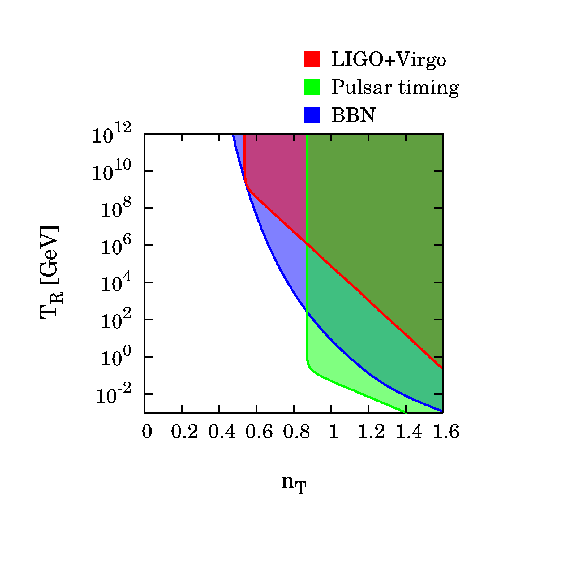
\includegraphics[width=0.75\linewidth, height=0.35\textheight]{Images/Chap3/Kurojanagi_Takahashi_Fig3}
	\caption{$ 2\sigma $ excluded region (colored) in the $ n_{T}-T_{R} $ plane for the case of the standard reheating scenario. The tensor-to-scalar ratio is assumed to be $ r=0.2 $ \cite{Chap3:BlueTiltedSpectrum}.}
	\label{fig:kurojanagitakahashifig3}
\end{figure}
\subsection*{Late-time entropy production}
In the case with late-time entropy production scenario, if large entropy is produced by the decay of another scalar field $\sigma$, the GW spectrum is further suppressed. The degree of suppression depends on the amount of the entropy produced, which is characterized by the diluition factor $ F $. The frequency range of the suppression depends on the temperature of the universe at the end of the second reheating $ T_{\sigma} $. Therefore, the bound on $ n_{T} $ depends on both $ F $ and $ T_{\sigma} $. The reheating temperature $ T_{R} $ is fixed  to be rather high as $ T_{R}=10^{15} $ GeV in order not to include the effect of the first reheating in the constraint on $ n_{T} $, and then simple see the effect of the late-time entropy production. In (Fig. \ref{fig:kurojanagitakahashifig4a}) and (Fig. \ref{fig:kurojanagitakahashifig5a}) are reported the excluded parameter space in the $ n_{T}-F $
 and $ n_{T}-T_{\sigma} $ planes. Since larger values of $ F $ give larger suppression of the GW spectrum, constraints from LIGO and BBN on $ n_{T} $ are weakened as $ F $ becomes large. On the other hand, we notice that the upper bound on $ n_{T} $ obtained from pulsar timing does not depend on the value of $ F $. This is because the constraint from pulsar timing is put at $ f \sim 10^{-8} $ Hz, which corresponds to  modes  which entered the horizon at $ T \sim 1 $ GeV. This involves that for the case of $ T_{\sigma} > 1 $ GeV the spectrum is suppressed at frequencies higher than $ f \sim 10^{-8} $ Hz, and then the constraint from pulsar timing is irrelevant to the value of $ F $.
 
Also in this model $ T_{\sigma} $ determines the frequency of the suppression of the spectrum. However, in contrast to the case of the standard reheating scenario, the suppression due to late-entropy production arises in a certain frequency range, which is determined by the amount of entropy production $ F $. Thus, the constraints on $ n_{T} $ from LIGO and BBN do not change depending on the value of $ T_{\sigma} $. The values $ F=10^{2} $ and $ 10^{5} $ assumed here are not enough to reduce the GW amplitude at high frequencies and to relax the observational bounds.

 Once the parameters $ T_{\sigma} $, $ F $, $ T_{R} $ and $ r $ are fixed, we can obtain an upper bound on $ n_{T} $ (see \cite{Chap3:BlueTiltedSpectrum}). An interesting fact is that BBN provides a stringest upper bound on $ n_{T} $ in most parameter space because the reheating temperature is assumed to be very high ($ T_{R}=10^{15} $ GeV) and the spectrum is not suppressed by reheating. Then BBN put strong constraints at very high frequencies. Instead, LIGO is sensitive at high frequencies ($\sim 100$ Hz ) and, as far as $ T_{\sigma} < 10^{10} $ GeV, the upper bound on $ n_{T} $ depends on the value of F and does not be affected by $ T_{\sigma} $. On the other hand, the pulsar timing has sensitivity at lower frequencies, $ f\sim 10^{-8} $ Hz, and when $ T_{\sigma} $ is below 0.1 GeV the suppression  becomes important at $ f\sim 10^{-8} $ Hz. 
\begin{figure}[h]
	\centering
	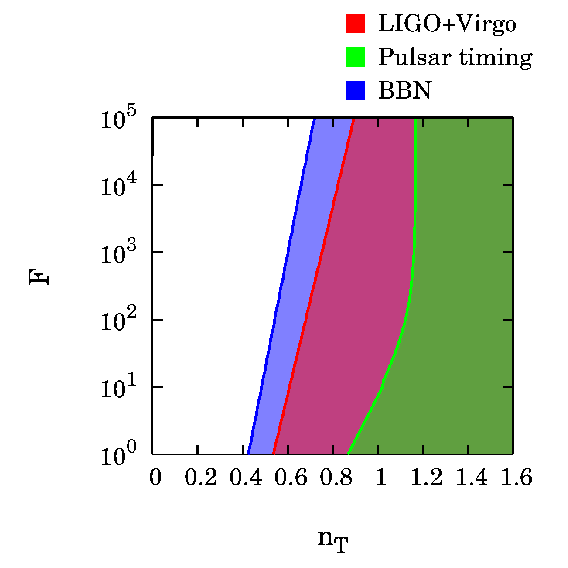
\includegraphics[width=0.45\linewidth, height=0.3\textheight]{Images/Chap3/Kurojanagi_Takahashi_Fig4A}
		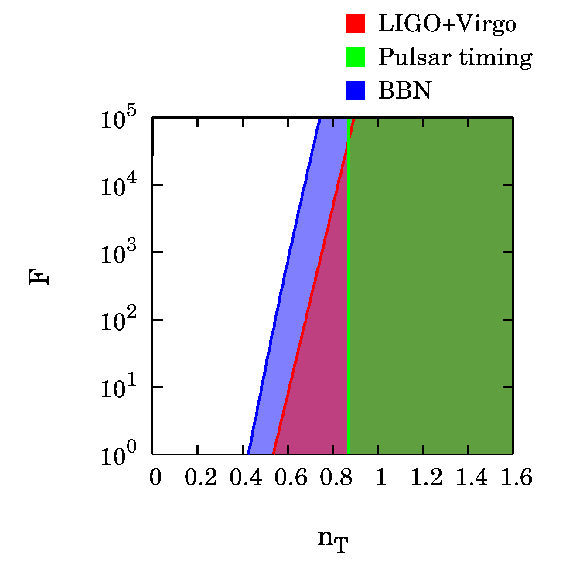
\includegraphics[width=0.45\linewidth, height=0.3\textheight]{Images/Chap3/Kurojanagi_Takahashi_Fig4B}
	\caption{$ 2\sigma $ excluded region (colored) in the $ n_{T}-F $ plane for the cases of $ T_{\sigma}=10^{-2} $ GeV(left) and $ 10^{3} $ GeV (right). We assume $ r=0.2 $ and $ T_{R}=10^{15} $ GeV \cite{Chap3:BlueTiltedSpectrum}. }
	\label{fig:kurojanagitakahashifig4a}
\end{figure}
\begin{figure}[h]
	\centering
	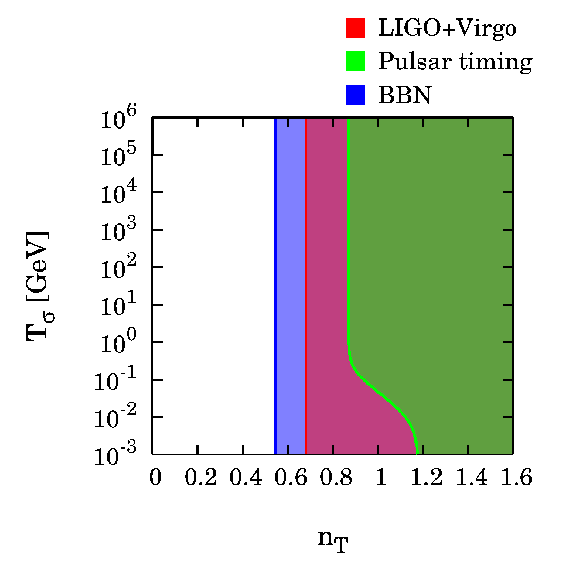
\includegraphics[width=0.45\linewidth, height=0.3\textheight]{Images/Chap3/Kurojanagi_Takahashi_Fig5A}
	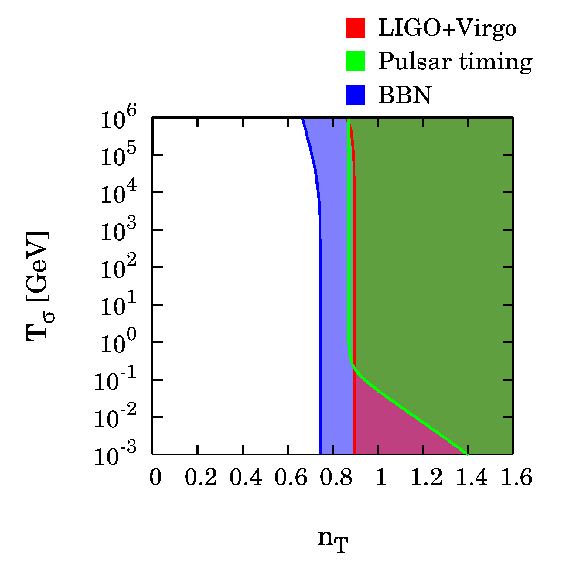
\includegraphics[width=0.45\linewidth, height=0.3\textheight]{Images/Chap3/Kurojanagi_Takahashi_Fig5B}
	\caption{$ 2\sigma $ excluded region (colored) in the $ n_{T}-T_{\sigma} $ plane for the cases of $ F=10^{2} $ GeV (left) and $ 10^{5} $ (right). We assume $ r=0.2 $ and $ T_{R}=10^{15} $ GeV \cite{Chap3:BlueTiltedSpectrum}.}
	\label{fig:kurojanagitakahashifig5a}
\end{figure}
\subsection{Extension to general case}
In the last part of this section we consider the most general case presented in \cite{Chap3:BlueTiltedSpectrum}. The stochastic GW spectrum is modeled by two parameters $\alpha$ and $ f_{\alpha} $, such that the power index of the spectrum changes from $ n_{T} $ to $\alpha$ at a characteristic frequency $ f_{\alpha} $. This approach covers a broad class of models of the early universe. For example, one can interpret the change of the power-law beheaviour as an effect of the change of the background evolution, which is applicable not only for reheating but also for different models. Moreover, we can adjust parameter values to describe a particular generation mechanism of primordial GW which does not predict a uniform spectral index over whole frequency range. 

The GW spectrum is modeled as 
\
\begin{equation}
	\large
		\label{Chap3:GWExtension}
	\Omega_{GW}(k) = 
	\begin{cases}
		\frac{1}{12}\Big ( \frac{k}{aH} \Big)^{2} T_{T}^{2}(k)A_{T}(k_{ref})\Big (\frac{k}{k_{ref}}\Big)^{n_{T}} \qquad  (k<k_{\alpha})\\		
		\frac{1}{12}\Big (\frac{k}{aH} \Big)^{2} T_{T}^{2}(k)A_{T}(k_{ref})\Big (\frac{k_{\alpha}}{k_{ref}}\Big)^{n_{T}}\Big (\frac{k}{k_{\alpha}}\Big)^{\alpha} \qquad  (k>k_{\alpha})
	\end{cases},
\end{equation}
where $ k_{\alpha} $ is the frequency at which the power index of the spectrum changes from $ n_{T}  $ to $\alpha$. The corresponding frequency is given by $ f_{\alpha}=k_{\alpha}/2\pi $. In this formula $ T_{T}^{2}(k) $ includes only $ T_{1}(k) $ (and not $ T_{2}(k) $ and $ T_{3}(k) $), which means  that only the change of the frequency dependence due to matter-radiation equality is included. The effect of reheating and late-time entropy production is excluded from the transfer function. This allows to treat in a more general way the change of the expansion rate before BBN.

An important application of this approach could be in the study of the equation of state during the reheating phase. Assume that the universe is dominated by a fluid whose equation of state parameter is $ \omega $. In the next section we will probe that a gravitational wave which enters the horizon during this phase has a spectral power dependence of
\begin{equation}
	\label{Chap3:OmegaEquationOfState}
	\Omega_{GW} \propto k^{\frac{2(3\omega - 1)}{1+3\omega}}.
\end{equation}
Therefore, when the background equation of state changes from $ \omega $ to $ 1/3 $ (radiation) at the temperature $ T_{\alpha} $, one can describe the GW spectrum by assuming $\alpha$ as 
\begin{equation}
\label{Chap3:dependence}
\alpha = \frac{2(3\omega-1)}{1+3\omega}	+ n_{T},
\end{equation}
and $ f_{\alpha} $ would be the quantity determined by $ T_{\alpha} $.
Moreover, this model can be applied also whenever in some models the spectral index changes from blue-tilted one to another.
This approach could be important when we consider the change of slope of the energy density spectrum of GW during the reheating epoch.

To have an intuitive idea of how the constraint on $ n_{T} $ depends on the value of $ \alpha $ and $ k_{\alpha} (f_{\alpha}) $ we show in (Fig. \ref{fig:kurojanagitakahashifig7}) the plot  in \cite{Chap3:BlueTiltedSpectrum} of the GW spectrum (\ref{Chap3:OmegaEquationOfState}). In the figure three examples of GW spectrum are shown, considering different scenarios of the early universe. First, a blue-tilted spectrum with $ n_{T} = 0.6 $, which underwent the standard reheating scenario with $ T_{R}=10^{6} $ GeV. Next, a scale invariant primordial spectrum in which the kinetic energy of a scalar field dominates the universe. Finally, a primordial spectrum  such that the model predicts a strongly blue-tilted spectrum of $ n_{T}=1 $ around the CMB scale, but at some later stage the situation becomes the same as the standard slow-roll inflation. 
In \cite{Chap3:BlueTiltedSpectrum} are presented also the contour plots in the $ f_{\alpha}-\alpha $ plane for each observational bound (LIGO, pulsar timing, BBN), which represent the upper bound on $ n_{T} $. Thus, once we know an approximated form  of the GW spectrum for some particular model, we can find the values of $\alpha$ and $ f_{\alpha} $ for that model and read off the upper bound on $ n_{T} $ from these plots (see the paper). 

Therefore, in this section we have seen a direct application of the reheting temperature.  It is found that the suppression of the GW spectrum due to reheating can significantly relax the constraints on the tensor spectral index $ n_{T} $, depending on the reheating temperature $ T_{R} $. Moreover, taking into account the late-time entropy production, the constraints on $ n_{T} $ changes depending on the amount of the produced entropy $ F $ and the cosmic temperature at the epoch of entropy production $ T_{\sigma} $. For example, assuming $ T_{R}=10^{15}  $ GeV, the constraints on $ n_{T} $ from BBN, LIGO and pulsar timing are $ n_{T} < 0.43,0.54 $ and $ 0.87 $ for $ r=0.2 $ at $ 95 \% $ C.L., respectevely. Assuming $ T_{R}=10^{6} $ GeV, instead, we obtain $ n_{T}<0.64,0.89,0.87 $ from BBN, LIGO and pulsar timing, respectevely \cite{Chap3:BlueTiltedSpectrum}.

\begin{figure}[h]
	\centering
	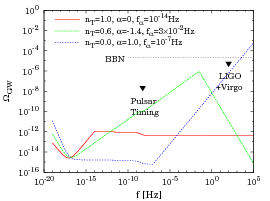
\includegraphics[width=0.7\linewidth, height=0.3\textheight]{Images/Chap3/Kurojanagi_Takahashi_Fig7}
	\caption{GW spectra modeled by $ \alpha $, $ f_{\alpha} $ \cite{Chap3:BlueTiltedSpectrum}.}
	\label{fig:kurojanagitakahashifig7}
\end{figure}

\section{Equation of State}
In the last sections we focused on the determination of the reheating temperature by observing the change of the frequency dependence of the GW spectrum. 

In the toy model of reheating showed in the previous chapter we assumed that, after inflation, the inflaton field behaves as non-relativistic matter with equation of state parameter $\omega = 0$. Thus, since this field still dominates the universe in this stage, the universe undergoes a matter-like era. 

We suppose now, in this model, that the inflaton beheaves during this phase as a generic perfect fluid with equation of state parameter $ \omega_{re} $.
We start rewriting the equation for the radiation during the reheating stage,
\begin{equation}
	\label{Chap3:radiationEquation}
	\dot{\rho_{r}} + 4H\rho_{r} = \Gamma_{\phi}\rho_{\phi}.
\end{equation}
Considering the general beheaviour of the scale factor, we can write
\begin{equation}
	\label{Chap3:ScaleFactorBeheaviour}
	\large
	a(t)=a_{osc}\Bigg(\frac{t}{t_{osc}}\Bigg)^{\frac{2}{3(1+\omega_{re})}},
\end{equation}
where $ a_{osc} \equiv a(t_{osc}) $ and $ t_{osc} $ is the time when the inflaton starts to oscillate around the minimum of its potential. During this stage the Hubble rate reads $ H=\frac{\dot{a}}{a}= \frac{2}{3(1+\omega_{re})t} $, and considering $\rho_{\phi} \sim a^{-3(1+\omega_{re})}$, (\ref{Chap3:radiationEquation}) becomes
\begin{equation}
	\label{Chap3:radiationEquationReheating2}
	\dot{\rho_{r}} + \frac{8}{3(1+\omega_{re})t}\rho_{r} = \Gamma_{\phi}\rho_{osc}\Bigg(\frac{a}{a_{osc}}\Bigg)^{-3(1+\omega_{re})},
\end{equation}
with $\rho_{r}(t_{osc})=0$ and $ \rho_{osc} = M^{4} $.
Before $ t \simeq \Gamma_{\phi}^{-1} $ the decay of the inflaton is not efficient. Using (\ref{Chap3:ScaleFactorBeheaviour}) we obtain
\begin{equation}
	\label{Chap3:TimeBeheaviour}
	\Bigg(\frac{a}{a_{osc}}\Bigg)^{-3(1+\omega_{re})} =  \Bigg(\frac{t}{t_{osc}}\Bigg)^{-2},
\end{equation}
and we set $ t_{osc}\simeq M_{pl}/M^{2} $. From (\ref{Chap3:radiationEquationReheating2}) the final equation to solve is
\begin{equation}
	\label{Chap3:FinalEquationRadiationReheating}
		\dot{\rho_{r}} + \frac{8}{3(1+\omega_{re})t}\rho_{r} = \frac{\Gamma_{\phi} M_{pl}^{2}}{t^{2}}.
\end{equation}
We solve this equation in the same way we did for the toy model of reheating. We write the general solution as
\begin{equation}
	\label{Chap3:GeneralSolutionReheating}
	\rho_{r}(t)=e^{-A(t)}\ \int_{t_{osc}}^{t} dt'(g(t')e^{A(t')}),
\end{equation}
where now $ A(t) $ is given by
\begin{equation}
	\label{Chap3:A(t)Parameter}
	A(t)=\frac{8}{3(1+\omega_{re})t},
\end{equation}
and the integral term now reads
\begin{equation}
	\label{Chap3:IntegralTermReheating}
	\int_{t_{osc}}^{t}\ dt' \frac{\Gamma_{\phi} M_{pl}^{2}}{t'^{2}}\Bigg(\frac{t'}{t_{osc}}\Bigg)^{\frac{8}{3(1+\omega_{re})}}=
	\frac{\Gamma_{\phi} M_{pl}^{2}}{t_{osc}^{8/3(1+\omega_{re})}}\int_{t_{osc}}^{t} dt'\ t'^{\frac{2(1-3\omega_{re})}{3(1+\omega_{re})}}.
\end{equation}
Solving the integral and putting all together in (\ref{Chap3:GeneralSolutionReheating}), we finally obtain
\begin{equation}
	\label{Chap3:radiationFinalSolutionTime}
	\rho_{r}(t)=\frac{\Gamma_{\phi}M_{pl}^{2}}{t}\Bigg(\frac{3(1+\omega_{re})}{5-3\omega_{re}}\Bigg)\Bigg(1-\Bigg(\frac{t}{t_{osc}}\Bigg)^{-\frac{5-3\omega_{re}}{3(1+\omega_{re})}}\Bigg).
\end{equation}
At $ t\simeq \Gamma_{\phi}^{-1} $ the decay becomes very efficient and we assume that the radiation era starts immediately. Equating the expression for the radiation density energy and (\ref{Chap3:radiationFinalSolutionTime}) at $ t \simeq \Gamma_{\phi}^{-1} $, we obtain an equation for the reheating temperature:
\begin{equation}
	\label{Chap3:EquatingRadiationThermalization}
\rho_{rad}=g_{*}\frac{\pi^{2}}{30}T_{reh}^{4}=\Gamma_{\phi}^{2}M_{pl}^{2}\Bigg(\frac{3(1+\omega_{re})}{5-3\omega_{re}}\Bigg),
\end{equation}
that yields
\begin{equation}
	T_{reh} \simeq 1.32\ g_{*}^{-1/4} (\Gamma_{\phi}M_{pl})^{1/2}\Bigg(\frac{3(1+\omega_{re})}{5-3\omega_{re}}\Bigg)^{1/4}.
\end{equation}
Thus, the reheating temperature has a dependence from the equation of state during reheating.

In general the equation of state is parametrized by a function $\omega_{re}(t)$ for the universe during the various stages of reheating. When inflation ends, $\omega_{re} = -1/3$. Assuming a massive inflaton, the equation of state climbs to 0. During this initial stage of reheating the frequency of oscillations, characterized by the inflaton mass, will be larger than the expansion rate. As the inflaton decays, the decay products compose an increasing percentage of the energy density of the universe,  increasing the equation of state parameter from 0 to 1/3 at the start of radiation dominance. However, it is estimated that during preheating (the initial stage of reheating) we have an increase of $ \omega_{re} $ from 0 to $\omega_{re} \sim 0.2-0.3$ \cite{Chap3:Podolsky_Felder}. However, the duration of this stage can be considered instantaneous in comparison with the remaining stages of reheating. Thus, in general $ \omega_{re} $ may be rightfully treated as a constant throughout the entire reheating era \cite{Chap3:Cook}.
\subsection{GW and equation of state}
We can relate the equation of state parameter $\omega$ to the tilt of the gravitational wave background spectrum. We assume that the initial power spectrum has no tilt, i.e. $ \Delta_{h,prim}^{2} \propto k^{0} $. Then, with this assumption, the frequency dependence of the spectrum is determined only by the transfer function. Therefore, from (\ref{Chap3:RelativeSpectralDensity2}) we have $\Omega_{GW} \propto k^{2}T^{2}_{T}(k)$.  A gravitational wave, with  initial amplitude of $ h_{\textbf{k},prim} $, mantains constant amplitude outside the horizon and it starts to decrease inversely proportional to the scale factor when the mode re-enters the horizon. Then, we can rewrite the transfer function as $ T_{T}(k) = |h_{\textbf{k,0}}|/|h_{\textbf{k},prim}| = (a_{0}/a_{in})^{-1} $, that implies $ \Omega_{GW} \sim k^{2}a^{2}_{in} $. We know that a mode re-enters the horizon  when $ k = aH $. Considering that the Hubble rate is given in terms of the equation of state as $ H^{2} \propto a^{-3(1+\omega)} $, we obtain $ a_{in} \propto k^{-2/(1+3\omega)} $. Thus, for modes which enter the horizon when the universe has the equation of state $\omega$, the spectrum has the frequency dependence of
\begin{equation}
	\label{Chap3:SpectrumFrequencyDependence}
	\Omega_{GW} \propto k^{\frac{2(3\omega - 1)}{3\omega + 1}}.
\end{equation} 
If we parametrize  the amplitude of the gravitational wave background spectrum, normalizing at $ f=F $, it reads
\begin{equation}
	\label{Chap3:SpectrumFrequencyDependenceParametrization}
	\Omega_{GW}(f) = \Omega_{GW,F}(f/F)^{\frac{2(3\omega - 1)}{3\omega + 1}}.
\end{equation}
Thus, from this equation we can easily see the change of slope of the spectrum at the reheating temperature in the case of the transition from the matter-like era after inflation to the radiation era. Indeed, matter-dominated era ($ \omega=0 $) and radiation-dominated era ($\omega=1/3$) corresponds to the frequency dependence $ f^{-2} $, $ f^{0} $, respectevely \cite{Chap3:ProspectsForDeterminationWithDetectors}. 

From the analysis of \cite{Chap3:ProspectsForDeterminationWithDetectors} results that the value of the tilt is more sensitive to the change of $\omega$ when the fiducial model is $ \omega \sim 0 $ than when $\omega$ has larger value. Then, it is easier for direct detection experiments  distinguish the model with smaller value of $\omega$.
\section{Informations from CMB}
Another possibility for extracting informations about reheating is to consider the expansion history of the universe between the time the observable CMB scales crossed outside the Hubble radius during inflation and the time they later re-entered. We can start by recapping the cosmic expansion history.

At early times the inflaton field $\phi$ drives the quasi-de-Sitter stage for $ N_{k} $ e-folds of expansion, while the reheating comoving horizon scale decreases as $ \sim a^{-1} $. The reheating phase starts when the accelerated expansion ends and the comoving horizon starts to increase. After another $ N_{re} $ e-folds of expansion the energy in the inflaton field has been completely dissipated into a hot plasma with a reheating temperature $ T_{re} $. After that, the universe expands under radiation domination for another $ N_{RD} $ e-folds before it makes the transition to the matter-dominated era. Thus, the number of e-folds between the time that the current comoving horizon scale exited the horizon during inflation and the end of inflation must be related to the number of e-folds between the end of inflation and today. Then, studying the expansion history of the universe we can trace the diluition of the energy density (Fig. \ref{fig:daikamionkowsifig1}) \cite{Chap3:Kai_Kamionkowsy}. 

\begin{figure}
	\centering
	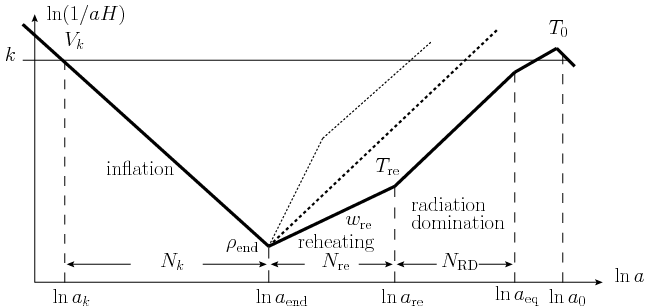
\includegraphics[width=0.8\linewidth, height=0.3\textheight]{Images/Chap3/Dai_Kamionkowsi_Fig1}
	\caption{The evolution of the comoving Hubble scale $ 1/aH $. The reheating phase connects the inflationary phase and the radiation era. Compared to instantaneous reheating (thick dotted curve), a reheating equation of state parameter $ \omega_{re}<1/3 $ implies more post-inflationary e-folds of expansion. Fewer post-inflationary e-folds requires $ \omega_{re} > 1/3 $ (thin dotted curve) \cite{Chap3:Kai_Kamionkowsy}.}
	\label{fig:daikamionkowsifig1}
\end{figure}
In this section we want find a connection between the CMB contraints on the primordial power spectrum (which would correspond to a prediction for $ N_{k} $) for a given inflationary model, and reheating parameters such as $ N_{re} $ (the duration of reheating). Moreover, for a given single-field inflationary model and for a given equation of state during reheating, we may use the CMB data to place constraints on the reheating temperature. We derive expressions for the reheating parameters $ (N_{re}$, $T_{re}$ and $ \omega_{re} $) in terms of a set of physical quantities that are specific to inflation and to the cosmological evolution subsequent to reheating (for reference see \cite{Chap3:Cook} and \cite{Chap3:Kai_Kamionkowsy}).

 Consider a single-field inflationary model with background field equation $ \ddot{\phi}+3H\dot{\phi} + V'=0 $. First, we derive an expression for $ N_{re} $. Assuming a constant equation of state during reheating,  the density energy of the universe beheaves as $ \rho \sim a^{-3(1+\omega_{re})} $. We write
\begin{equation}
	\label{Chap3:DensityEnergyBeheaviour}
	\frac{\rho_{end}}{\rho_{re}}=\Bigg( \frac{a_{end}}{a_{re}}\Bigg)^{-3(1+\omega_{re})},
\end{equation}
where the subscripts \textit{end} and \textit{re} denote, respectevely, the end of inflation and the end of reheating. In terms of e-foldings, $ N_{re}=ln(a_{re}/a_{end}) $, we obtain
\begin{equation}
	\label{Chap3:Nre}
	N_{re}=\frac{1}{3(1+\omega_{re})}\ln\Bigg(\frac{\rho_{end}}{\rho_{re}}\Bigg).
\end{equation}
For example,  consider for the inflaton power-law potentials
\begin{equation}
	\label{Chap3:potentialInflation}
	V(\phi)=\frac{1}{2}m^{4-\alpha}\phi^{\alpha},
\end{equation}
with power-law $\alpha$ and mass parameter $ m $. We can determine the number of e-folds $ N_{k} $ from the time that the field value is $\phi_{k}$ until the end of inflation $ \phi_{end} $: 
\begin{equation}
	\label{Chap3:N_{k}}
	N_{k}=\int_{t_{k}}^{t_{end}} H dt = \int_{\phi_{k}}^{\phi_{end}}\frac{H}{\dot{\phi}}d\phi.
\end{equation}
Using the equation of motion  $\dot{\phi} \simeq -V'(\phi)/3H $ and $ H^{2}\simeq (8\pi /3M_{pl}^{2})V(\phi) $ during inflation, we obtain
\begin{equation}
	\label{Chap3:eFolds}
	N_{k}=-\int_{\phi_{k}}^{\phi_{end}}\Bigg(\frac{8\pi \phi}{M_{pl}^{2}\alpha}\Bigg)d\phi = \frac{\phi^{2}_{k} - \phi^{2}_{end}}{2\alpha M_{pl}^{2}} \simeq \frac{\phi_{k}^{2}}{2\alpha M_{pl}^{2}},
\end{equation}
where we have assumed that the field value at the end of inflation $\phi_{end}$ is small compared to that during the slow-roll. 

For this model we can find also a simple relation for the slow-roll parameters
\begin{equation}
	\label{Chap3:slowRollParameters}
	\epsilon \simeq \frac{M_{pl}^{2}}{2}\Bigg(\frac{V'(\phi)}{V(\phi)}\Bigg)^{2},
	\qquad
	\eta \simeq M_{pl}^{2}\Bigg(\frac{V''}{V}\Bigg).
\end{equation}
Using the relation (\ref{Chap3:eFolds}), the slow-roll parameters can be simply rewritten in this model as
\begin{equation}
	\label{Chap3:slowRollParameters2}
	\epsilon_{k} = \frac{\alpha}{4N_{k}}
	\qquad
	\eta_{k}=\frac{\alpha-1}{2N_{k}},
\end{equation}
where they are evaluated at the reference scale $ k $. Finally, we obtain a simple relation also for the spectral tilt at the scale $ k $:
\begin{equation}
	\label{Chap3:spectralTilt}
	n_{s}-1=-6\epsilon + 2\eta = -\frac{\alpha + 2}{2N_{k}}.
\end{equation}

In Cosmology we observe perturbation modes on scales that are comparable to that of the horizon. For reference scale we choose the pivot scale at which Planck determines $ n_{s} $, $ k=0.05 $ Mpc$ ^{-1} $. The comoving Hubble scale $ a_{k}H_{k}=k $, when this mode exited the horizon, can be related to that of the present time by means
\begin{equation}
\label{Chap3:relationBetweenScales}
\frac{k}{a_{0}H_{0}} = \frac{a_{k}}{a_{end}}\frac{a_{end}}{a_{re}}\frac{a_{re}}{a_{eq}}\frac{a_{eq}H_{eq}}{a_{0}H_{0}}\frac{H_{k}}{H_{eq}},
\end{equation} 
where quantities with subscript k are evaluated at the time of the horizon exit. Same thing for the other subscripts: end of inflation (end), end of reheating (re), radiation-matter equality (eq) and the present time (0). Then, we use $ e^{N_{k}}=a_{end}/a_{k},\ e^{N_{re}}=a_{re}/a_{end}  $ and $ e^{N_{RD}}=a_{eq}/a_{re} $ to obtain a constraint on the total amount of expansion,
\begin{equation}
	\label{Chap3:relationBetweenScales2}
	\ln \Bigg(\frac{k}{a_{0}H_{0}}\Bigg) = -N_{k} - N_{re} - N_{RD} + \ln \Bigg(\frac{a_{eq}H_{eq}}{a_{0}H_{0}}\Bigg) + \ln \Bigg(\frac{H_{k}}{H_{eq}}\Bigg).   
\end{equation}
To solve this equation we first  write an expression for $ H_{k} $ as a function of $ n_{s} $. Using the definition of the tensor-to-scalar ratio $ r= P_{h}/P_{\zeta} $, with $ P_{h}=(2H^{2})/(\pi^{2}M_{pl}^{2}) $ and $ P_{\zeta} = A_{s} $ at the pivot scale, 
\begin{equation}
\label{chap3:tensortToScalarRatio}
r_{k}=\frac{2H^{2}_{k}}{\pi^{2}M_{pl}^{2}A_{s}}.
\end{equation}
Using the consistency relation $ r=16\epsilon $, we obtain
\begin{equation}
	H_{k}\simeq \pi M_{pl}\sqrt{8A_{s}\epsilon_{k}}.
\end{equation}
We can then express $ H_{k} $ in terms of the spectral tilt $ n_{s} $, the power-law index $\alpha$ and $ A_{s} $, using (\ref{Chap3:spectralTilt}) and (\ref{Chap3:slowRollParameters2}). The expression for $ H_{k} $ becomes
\begin{equation}
	\label{chap3:expressionHk}
	H_{k}=\pi M_{pl}\sqrt{\frac{2A_{s}\alpha (1-n_{s})}{\alpha +2}}.
\end{equation}
The energy density at the end of reheating determines the reheating temperature through $\rho_{re}=(\pi^{2}/30)g_{re}T^{4}_{re}$. The subsequent expansion is mainly driven by hot radiation, except for very recently non-relativistic matter and dark energy. Thus, for semplicity, we assume that no immense entropy production occurs after $ T_{re} $. Under this assumption the reheating entropy is preserved in the CMB-neutrino background today, and leads to the relation
\begin{equation}
	\label{Chap3:relationEntropy}
	g_{s,re}T_{re}^{3}a_{re}^{3}=g_{0s}T_{0}^{3}a_{0}^{3},
\end{equation}
from which
\begin{equation}
	\label{Chap3:relationEntropy2}
	g_{s,re}T_{re}^{3} = \Bigg(\frac{a_{0}}{a_{re}}\Bigg)^{3}\big(2T_{0}^{3} + 6 \cdot \frac{7}{8} \cdot T_{\nu 0}^{3}\big),
\end{equation}
where $ T_{0}=2.725  $ K is the present CMB temperature, and $ T_{\nu,0}=(4/11)^{1/3}\ T_{0} $ is the neutrino temperature. $ g_{re} $ is the effective number of degrees of freedom at the end of reheating. From  (\ref{Chap3:relationEntropy2}) we can derive a relation between  today CMB-temperature $ T_{0} $ and the reheating temperature $ T_{re} $:
\begin{equation}
\label{Chap3:RelationReheatingToday}
\frac{T_{re}}{T_{0}}=\Bigg(\frac{43}{11g_{s,re}}\Bigg)^{1/3}\frac{a_{0}}{a_{eq}}\frac{a_{eq}}{a_{re}}.
\end{equation}
Using $ e^{-N_{RD}} = a_{re}/a_{eq}$, we rewrite the reheating temperature as
\begin{equation}
\label{Chap3:ReheatingTemperature}
T_{re} = T_{0}\Bigg(\frac{43}{11 g_{s,re}}\Bigg)^{1/3}\Bigg(\frac{a_{0}}{a_{eq}}\Bigg)e^{N_{RD}}.
\end{equation}
We also rewrite $ a_{0}/a_{eq} $ using (\ref{Chap3:relationBetweenScales}),
\begin{equation}
\label{Chap3:a0/aeq}
\frac{a_{0}}{a_{eq}}= \frac{a_{0}H_{0}}{k}\frac{a_{k}}{a_{end}}\frac{a_{end}}{a_{re}}\frac{a_{re}}{a_{eq}}\frac{H_{eq}}{H_{0}}\frac{H_{k}}{H_{eq}},
\end{equation}
that leads
\begin{equation}
\frac{a_{0}}{a_{eq}}= \frac{a_{0}H_{k}}{k}e^{-N_{k}}e^{-N_{re}}e^{-N_{RD}}.
\end{equation}
With this expression for $ a_{0}/a_{eq} $, we can finally rewrite the reheating temperature as
\begin{equation}
	\label{Chap3:reheatingTemperature3}
	T_{re} = T_{0}\Bigg(\frac{43}{11 g_{s,re}}\Bigg)^{1/3}\Bigg( \frac{a_{0}H_{k}}{k} \Bigg)e^{-N_{k}}e^{-N_{re}}.
\end{equation}
From this relation we see that larger values of $ N_{re} $ corresponds to smaller $ T_{re} $ and viceversa. In other words, quicker and more efficiently reheating takes place, larger becomes the reheating temperature. 

We use now the fact that, at the end of inflation, the equation of state has to be $ \omega_{end}=-1/3 $ to stop the exponential quasi-de-Sitter expansion ($\omega_{inf} \simeq -1$). At this time then we have that the energy density and the pressure of the inflaton read
\begin{equation}
	\rho_{end} = \frac{1}{2}\dot{\phi^{2}} + V_{end}(\phi),
	\qquad
	P_{end}=  \frac{1}{2}\dot{\phi^{2}} - V_{end}(\phi),
\end{equation}
with the equation of state $ P_{end}=\omega_{end}\ \rho_{end}=-(1/3)\rho_{end} $, and the inflaton potential evaluated at the end of inflation. Using the equation of state at the end of inflation and  these expressions, we obtain 
$ -\frac{1}{3}\rho_{end}= \frac{1}{2}\dot{\phi^{2}}-V_{end} $. Using also $ \frac{1}{2}\dot{\phi^{2}}=\rho_{end}-V_{end} $, we obtain the simple relation 
\begin{equation}
	\label{Chap3:energyDensityPressure}
	\rho_{end}=\frac{3}{2}V_{end}.
\end{equation}
Plugging this into $ N_{re}=\frac{1}{3(1+\omega_{re})}\ln(\rho_{end}/\rho_{re})$, $ N_{re} $ becomes
\begin{equation}
\label{Chap3:Nre2}
N_{re}=\dfrac{1}{3(1+\omega_{re})}\ln \Bigg(\frac{3 V_{end}}{2\rho_{re}} \Bigg) = \dfrac{1}{3(1+\omega_{re})}\ln \Bigg( \frac{30 \cdot \frac{3}{2} V_{end}}{\pi^{2}g_{re}T^{4}_{re}}\Bigg).
\end{equation}
Finally, using the expression found for the reheating temperature (\ref{Chap3:reheatingTemperature3}), it reads
\begin{equation}
\label{Nre3}
N_{re}=\frac{4}{3(1+\omega_{re})}\Bigg[  \frac{1}{4} \ln \Bigg(\frac{45}{\pi^{2} g_{re}}\Bigg)   + \ln \Bigg(\frac{V_{end}^{1/4}}{H_{k}}\Bigg) +  \frac{1}{3}\ln \Bigg(\frac{11 g_{re}}{43}\Bigg) + \ln \Bigg(\frac{k}{a_{0}T_{0}}\Bigg) + N_{k} + N_{re}    \Bigg].
\end{equation}
Solving this in terms of $ N_{re} $, assuming $ \omega_{re} \ne 1/3 $, we find
\begin{equation}
	\label{Chap3:Nre3}
	N_{re}=\frac{4}{3(1-\omega_{re})}\Bigg[ - \frac{1}{4} \ln \Bigg(\frac{45}{\pi^{2} g_{re}}\Bigg)   - \ln \Bigg(\frac{V_{end}^{1/4}}{H_{k}}\Bigg) -  \frac{1}{3}\ln \Bigg(\frac{11 g_{re}}{43}\Bigg) - \ln \Bigg(\frac{k}{a_{0}T_{0}}\Bigg) - N_{k}     \Bigg].
\end{equation}
The second and the last terms in the right part of this equation depend on the specific inflationary model, since $ V_{end} $ is the potential of the inflaton evaluated at the end of inflation, and $ N_{k} $ is the number of e-folds between the pivot scale $ k $ crosses outside the Hubble radius and the time when inflation ends. Assuming $ g_{re} \simeq 100 $ and using Planck's pivot scale of $ 0.05 $ Mpc$^{-1}$, one obtains a simplified expression for $ N_{re} $, without specifying a particular inflationary model:
\begin{equation}
	\label{Chap3:NreFinalForm}
	N_{re}=\frac{4}{(1-3\omega_{re})}\Bigg[61.6 - \ln \Bigg( \frac{V_{end}^{1/4}}{H_{k}}\Bigg) - N_{k}     \Bigg].
\end{equation}
Moreover, plugging this equation into (\ref{Chap3:reheatingTemperature3}), we can find another expression for the reheating temperature,
\begin{equation}	
T_{re} = \Bigg[\Bigg(\frac{43}{11g_{re}}\Bigg)^{1/3}\frac{a_{0}T_{0}}{k}H_{k}e^{-N_{k}}\Big[\dfrac{45 V_{end}}{\pi^{2}g_{re}}\Big]^{-\frac{1}{3(1+\omega_{re})}}\Bigg]^{\frac{3(1+\omega_{re})}{3\omega_{re}-1}}.	
\end{equation}
The results obtained for $ N_{re} $ in (\ref{Chap3:NreFinalForm}) and (\ref{Chap3:Nre3}) are valid only if $\omega_{re} \ne 1/3$. Indeed, if $\omega_{re}=1/3$ in  (\ref{Chap3:Nre3}), $ N_{re} $ cancels from both sides of the equation. Assuming $ g_{re} = 100 $ and Planck's pivot scale, one finds \cite{Chap3:Cook}
\begin{equation}
	61.6 = \ln \Bigg( \frac{V_{end}^{1/4}}{H_{k}}\Bigg) + N_{k}.
\end{equation}
The issue is that we are defining the start of radiation dominance as the moment in which $\omega_{re}=1/3$. If $\omega_{re}$ is already equal to $ 1/3 $ during the reheating phase, then there is ambiguity in differentiating the two regimes. This implies that for $\omega_{re}=1/3$ is not possible to derive a prediction for $ N_{re} $ or $ T_{re} $ but, instead, for a particular inflation model, one finds a prediction for $ n_{s} $.

Going back to the inflaton potential $ V(\phi)=\frac{1}{2}m^{4-\alpha}\phi^{\alpha} $, we have found the expression for $ N_{k}=\frac{\alpha + 2 }{2(1-n_{s})} $, $ H_{k}=\pi M_{pl}\big(\frac{4\pi A_{s}(1-n_{s})}{\alpha +2}\big)^{1/2} $ in terms of $\alpha$, $ n_{s} $ and $ A_{s} $.
 We finally compute also $ V_{end} $ in terms of $ n_{s} $ and $ A_{s} $. To find $ V_{end} $ we start from the expression for $ H_{k} $ in terms of the potential
 \begin{equation}
\label{Chap3:HubblekPotential}
H_{k}\simeq  \frac{8\pi}{3M_{pl}^{2}}V(\phi_{k})= \frac{8\pi}{3M_{pl}^{2}}\frac{1}{2}m^{4-\alpha}\phi_{k}^{\alpha},
 \end{equation}
from which $ m^{4-\alpha} \simeq \frac{6M_{pl}^{2}H_{k}}{8\pi \phi_{k}^{\alpha}} $.
On the other hand, $ V_{end}=\frac{1}{2}m^{4-\alpha}\phi_{end}^{\alpha} $. Substituing in $ V_{end} $ the expression found for $ m^{4-\alpha} $, we obtain
\begin{equation}
	\label{Chap3:Vend}
	V_{end}=3M_{pl}^{2}H_{k}\Big(\frac{\phi_{end}}{\phi_{k}}\Big)^{\alpha}.
\end{equation}
The value of the field at the end of inflation is computed imposing the slow-roll condition $\epsilon = 1$. From (\ref{Chap3:slowRollParameters2}) we have that $\epsilon_{end}\simeq 1$ implies $\alpha = 4N= 4 \phi^{2}_{end}/2\alpha$, that yields
\begin{equation}
	\label{Chap3:phiEnd}
\phi_{end}\simeq\frac{\alpha M_{pl}}{\sqrt{2}}.
\end{equation}
Using also (\ref{Chap3:spectralTilt}),
\begin{equation}
\label{Chap3:expressionN_{k}}
\phi_{k}^{2}=2\alpha M_{pl}^{2}N_{k}=2\alpha M_{pl}^{2}\frac{\alpha + 2}{2(1-n_{s})},
\end{equation}
and, finally considering also the expression for $ H_{k} $ (\ref{chap3:expressionHk}), $ V_{end} $ reads
\begin{equation}
\label{Chap3:Vend2}
V_{end}=6\pi^{2}M_{pl}^{4}A_{s}(1-n_{s})\Bigg(\frac{\alpha(1-n_{s})}{2(\alpha+2)}\Bigg).
\end{equation}
Thus $ N_{k},\ H_{k}$ and $ V_{end} $ are all expressed as functions only of $ \alpha $, $ n_{s} $ and $ A_{s} $. One can then plot $ N_{re} $ or $ T_{re} $ as a function of $ n_{s} $ for some fixed values of $ \omega_{re} $ and $ \alpha $. We consider $ n_{s}=0.9682 \pm 0.0062 $ and Planck's central value $ A_{s}=2.196\times 10^{-9} $. Moreover, in general once the form of the inflaton potential is specified for a given model, one can express $ V_{end} $ as a function of model parameters calculated at the pivot scale. One can also use $ V_{end} $ to derive $ N_{re} $ and $ T_{re} $ as a function of inflationary model parameters using the equations found in this section \cite{Chap3:Cook}.
\subsection{Results}
We report the results of \cite{Chap3:Cook} and \cite{Chap3:Kai_Kamionkowsy}.
\begin{figure} [h]
	\centering
	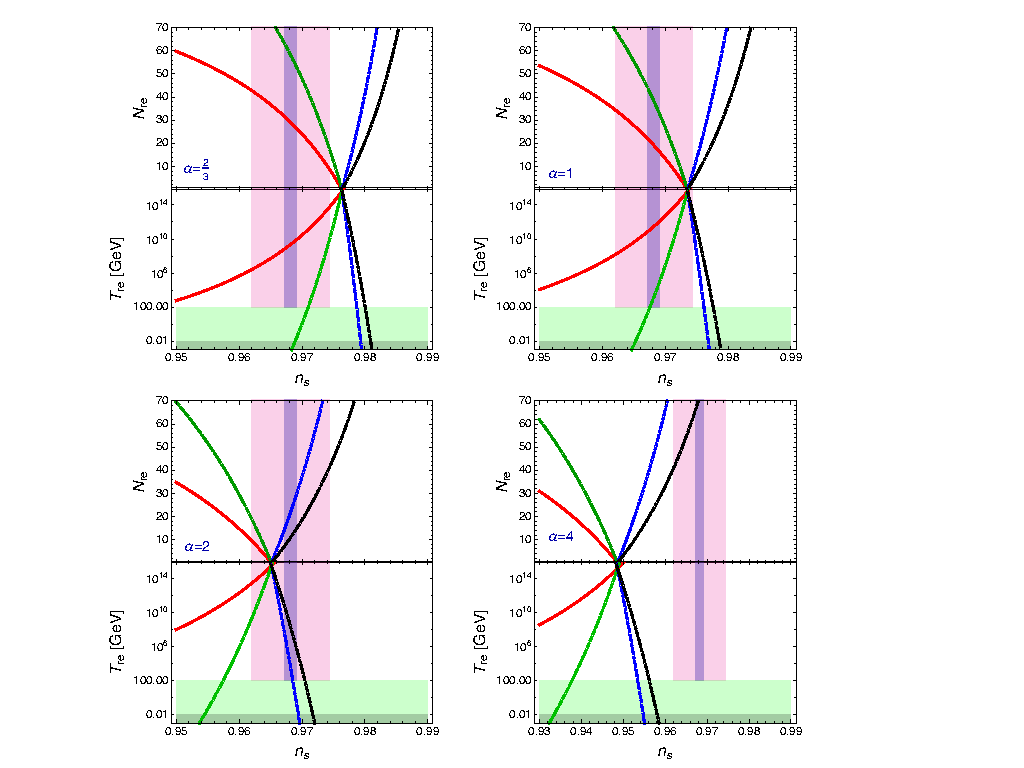
\includegraphics[width=1\linewidth, height=0.3\textheight]{Images/Chap3/Cook_Fig.2}
	\caption{Plots of $ N_{re} $ and $ T_{re} $, the length of reheating and the temperature at the end of reheating, respectively, for polynomial potentials with exponent $\alpha$. The solid red line corresponds to $ \omega_{re}=-1/3 $, the dashed green line to $\omega_{re}=0$, the dotted blue line to $ \omega_{re}=2/3 $, and the dot-dashed black line to $\omega_{re}=1$. The pink shaded region corresponds to the $ 1\sigma $ bounds on $ n_{s} $ from Planck. The purple shaded region corresponds to the $ 1\sigma $ bounds of a further CMB experiment with sensitivity $ 10^{-3} $, using the same central $ n_{s} $ value as Planck. Temperatures below the dark green shaded region are ruled out by BBN. The light green shaded region is below the electroweak scale, assumed 100 GeV for reference. This region is not disallowed but would be interesting in the context of baryogenesis \cite{Chap3:Cook}. }
	\label{fig:cookfig}
\end{figure}
 In (Fig. \ref{fig:cookfig}) from \cite{Chap3:Cook} are computed $ N_{re} $ and $ T_{re} $ as functions of $ n_{s}-1 $ for power-law potentials with $\alpha=2/3,1,2,4$. The results indicate that the quadratic potential $\alpha=2$ implies a prolonged reheating epoch for the central value $ n_{s} \simeq 0.96 $ and canonical reheating ($ \omega_{re} = 0 $). It is required a reheating temperature $ T_{re}\simeq 10^{6} $, and a number $ N_{re} \simeq 30 $ of e-folds in this case. Instead, a scalar tilt bluer than 0.96 requires smaller $ N_{re} $ and higher reheating temperature. In \cite{Chap3:Kai_Kamionkowsy}  is derived from  numerical analysis a relation between the reheat temperature $ T_{re} $ and the scalar spectral index $ n_{s} $, given by $ \log_{10}(T_{re}/10^{6}GeV) \simeq 2000(n_{s}-0.96) $. From this formula we see that an higher reheat temperature $ T_{re} $ implies a larger $ n_{s} $. If $ T_{re} $ is considerably above the electroweak scale, then $ n_{s} $ will have to be larger than its central value. For example, if reheating was nearly instantaneous and set $ T_{re}\simeq 10^{16} $ GeV, as may required by GUT-scale baryogenesis models, then quadratic inflation requires $ n_{s}\simeq 0.965 $ (taking $ k=0.05 Mpc^{-1} $ used by Planck. This value increase to $ n_{s} \simeq 0.967 $ for the WMAP pivot scale $ k=0.02 Mpc^{-1} $ ).
 
For models with smaller power-law indeces ($ \alpha=2/3,1 $) canonical reheating is too efficient in diluiting the energy density if $ n_{s} $ falls within its $ 1\sigma $ error range. These types of model (axion-monodromy models), unless $ n_{s} $ is above the current $ 1\sigma  $ upper limit, require some exotic mechanism of reheating, beyond that in the canonical scenario. On the other hand, models with larger power-law potentials indeces ($\alpha=3,4$), require $\omega_{re} > 1/3 $ (irrealistic considering that this would mean a diluition of energy density faster than that occurs during the radiation epoch). Thus, also in these models reheating  require some non-canonical picture, unless $ n_{s} $ is near the lower limit of the current $ 2\sigma $ range.

In conclusion, the analysis suggests that the power-law inflationary models, with $ \alpha=2 $, are the most compatible with the simplest canonical reheating scenario. The current data then do seem to favor a simple quadratic inflaton potential if a simple reheating scenario is assumed \cite{Chap3:Cook}.

In \cite{Chap3:Cook} is studied, with the approach discussed in this section, a broad range for the equation of state parameter, $ -1/3 \le \omega_{re} \le 1 $,  with the corresponding limits on CMB observables for different inflationary models. From the analysis comes out that a $\phi^{2}$ potential would favor relatively large values of $ r $. For example, a reheating model with $ \omega_{re} \le 1 $ imples $ r\ge 0.11 $. On the other hand, to allow a reheating model with $\omega_{re} \le 1/3$, which is very probable, the tensor-to-scalar ratio requires to be $ r\ge 0.14 $. For natural inflation, considered in the previous chapter, the paper finds that  Planck's $ 2\sigma $ bound on $ n_{s} $ favors a tensor-to-scalar ratio $ r\ge 0.05 $ for $ \omega_{re} \le 1/3 $.
 \section{Bayesian approach}
 We end this chapter considering the Bayesian approach to have informations about reheating using CMB. So far, the contraints on the reheating temperature and the reheating energy scale are not so numerous. The reheating temperature should be less than $ 10^{16}  $ GeV, and also should proceed before BBN implying $ T_{reh} \ge 10 $ MeV. Thus, the reheating temperature is poorly constrained, in particular its lower limit.
 
 In \cite{Chap3:Martin_Ringeval} are derived constraints on the reheating phase making use of Bayesian techniques and utilizing a full numerical approach. This approach has several advantages. First, the method remains accurate when the slow-roll approximation breaks down, as one expects near the end of inflation. Second, it permits a new treatment of reheating. Indeed, instead of viewing the reheating parameters as a nuisance collection of parameters, they can easily be included in the Bayesian data analysis process. Third, the evolution of cosmological perturbations in the hot Big-Bang theory already relies on numerical codes. Treating perturbations during inflation in the same way allows to automatize the entire procedure and easily extends to other scenarios. Fourth, the numerical approach allows us to solve the problem of the prior choice. Indeed, from a physical point of view, our prior knowledge is on the inflationary theory and not the shape of the primordial power-spectra which is actually a model prediction. Therefore, it is better and easier to choose prior probability distributions directly on model parameters, such as the power index of the large-field potentials \cite{Chap3:Martin_Ringeval}.
 
 In this section we only outline the main points. For a complete treatment see \cite{Chap3:Martin_Ringeval}, where the Bayesian approach was first introduce to study reheating, \cite{Chap3:Martin_Observing_Reheating} which is based on Planck 2013 data, and \cite{Chap3:Martin_Milestone} based on Planck 2015 data (using a better analysis).
 
 The evolution of scalar density perturbation is described by the Mukhanov-Sasaki variable $ v_{k} $, seen in the first chapter (in accordance with the literature, we renamed $ \mathcal{Q}_{k} $ with $ v_{k} $ ). The equation (\ref{finalEOM}) can be rewritten in terms of the slow-roll parameter $\epsilon$:
 \begin{equation}
\label{Chap3:equationScalarPerturbations}
v_{k}'' + \Bigg[k^{2} - \frac{(a\sqrt{\epsilon})''}{a\sqrt{\epsilon}}\Bigg]v_{k}=0.
 \end{equation}
The Mukhanov-Sasaki variable $ v_{k} $ is related to the curvature pertubation $\zeta_{k}$ through the following relation
\begin{equation}
	\label{Chap3:Zetak}
	\zeta_{k} = \frac{1}{M_{pl}}\frac{v_{k}}{a\sqrt{2\epsilon}},
\end{equation}
from which we derive the power spectrum of $ \zeta_{k} $,
\begin{equation}
	\label{Chap3:PowerSpectrum}
	P_{\zeta_{k}} \equiv \frac{k^{3}}{2\pi^{2}}|\zeta_{k}|^{2}=\frac{k^{3}}{4\pi^{2}M_{pl}^{2}}\Bigg|\frac{v_{k}}{a\sqrt{\epsilon}}\Bigg|^{2}.
\end{equation}
To obtain the power sperctrum $ P_{\zeta}(k) $ one has to integrate (\ref{Chap3:equationScalarPerturbations}) with initial conditions given by the Bunch-Davis vacuum 
\begin{equation}
	\label{Chap3:BunchDavis}
	\lim_{k/\mathcal{H} \rightarrow +\infty} v_{k} = \frac{1}{\sqrt{2k}}e^{-ik\tau},
\end{equation}
since, at the beginning of inflation, all the modes of astrophysical interest today were much smaller than the Hubble radius.

As said in the first chapter, the curvature perturbation $\zeta_{k}$ is directly linked to CMB anisotropies and it is a conserved quantity on large scales. This means that one can use it to propagate the inflationary spectrum from the end of inflation to the post-inflationary era. In other words, the power spectrum is not affected by the post-inflationary evolution, in particular by the reheating stage. However, in the previous section we have seen that the relation between the physical scales at present and during inflation depends on the properties of the reheating epoch. Thus, in order to calibrate the inflationary spectrum with respect to the physical scales of astrophysical interest today, we need to know how reheating proceed.

We can express (\ref{Chap3:equationScalarPerturbations}) in terms of the number of e-folds during inflation, $ N=\ln (a/a_{in}) $, where $ a_{in} $ is the value of the scale factor at the beginning of inflation. It can be written as 
\begin{equation}
\label{Chap3:scalarPerturbation}
\frac{d^{2} v_{\textbf{k}}}{dN^{2}} + \frac{1}{\mathcal{H}}\frac{d\mathcal{H}}{dN}\frac{dv_{\textbf{k}}}{dN} + \Bigg[\Bigg(\frac{k}{\mathcal{H}}\Bigg)^{2}-U_{s}(N)\Bigg]v_{\textbf{k}}=0,
\end{equation}
where $ U_{s}(N) $ is an effective potential for the perturbations which depends on the scale factor and its derivative only. All the terms in the equation, but $ k/\mathcal{H} $, are specified by the inflationary background evolution. Given  a physical scale today, say $ k/a_{now}=0.05 $ Mpc$^{-1} $, we need to express $ k/\mathcal{H} $ in terms of $ k/a_{now} $ and quantities defined during inflation. We can find then the relation
\begin{equation}
\label{Chap3:kH}
\frac{k}{\mathcal{H}}=\frac{\Gamma_{k}}{H(N)}e^{N_{T}}e^{-N},
\end{equation}
where $ N_{T} $ is the total number of e-folds during inflation. In \cite{Chap3:Martin_Ringeval} was defined $\Gamma_{k}$ as
\begin{equation}
	\label{Chap3:Gammak}
	\Gamma_{k}\equiv \frac{k}{a_{now}}(1+z_{now}) = \frac{k}{a_{now}}\Bigg(\frac{\rho_{end}}{\Omega_{\gamma}\rho_{cr}}\Bigg)^{1/4}R^{-1}_{rad},
\end{equation}
where in the paper was introduced the new parameter $ R_{rad} $. This parameter plays a crucial role in this treatment. $\rho_{end}$ is the energy density at the end of inflation, $\rho_{cr}$ is the present day critical energy density and $\Omega_{\gamma} \simeq 2.471 \times 10^{-5} h^{-2}$ is the density parameter of radiation today.
The parameter $ \Gamma_{k} $ depends on the whole post-inflationary evolution of the universe through $ z_{end} $. After inflation only the reheating phase is poorly known and represents the main source of uncertainty for the inflationary predictions.

In order to find the physical interpretation of $ R_{rad} $, assume that the reheating phase is dominated by a conserved effective fluid with energy density $\rho$ and pressure $ P $, with the equation of state parameter $\omega_{re}$.  We can define the energy density during reheating as
\begin{equation}
	\label{Chap3:energyDensityDuringReheating}
	\rho(N) = \rho_{end} \exp \Biggl\{-3 \int_{N_{T}}^{N}[1+\omega_{re}(n)]dn\Biggr\}.
\end{equation}
From this expression we can derive
\begin{equation}
\label{Chap3:lnRad}
\ln R_{rad} = \frac{\Delta N}{4}(-1 + 3\bar{\omega}_{re}),
\end{equation}
where 
\begin{equation}
	\Delta N \equiv N_{re} - N_{T}
\end{equation}
is the total number of e-folds during reheating, being $ N_{re} $ the number of e-folds at which reheating is completed and the radiation dominated era begins. The parameter $\bar{\omega}_{re}$ denotes the mean equation of state parameter
\begin{equation}
\label{Chap3:meanEqStateParametere}
\bar{\omega}_{re}\equiv \frac{1}{\Delta N}\int_{N_{T}}^{N_{re}}\omega_{re}(n)dn.
\end{equation}
Then, the parameter $ R_{rad} $  only depends on what happens during reheating. In the special case  in which $ \bar{\omega}_{re}=1/3 $, $ \ln R_{rad}=0 $ and, in this case, the reheating stage cannot be distinguished from the subsequent radiation dominated era and cannot affect the inflationary predictions. This also implies $ R_{rad}=1 $.

From (\ref{Chap3:energyDensityDuringReheating}) $ \ln R_{rad} $ can be put in the form
\begin{equation}
\label{Chap3:Rrad2}
\ln R_{rad}= \frac{1-3\bar{\omega}_{re}}{12(1+\bar{\omega}_{re})}\ln \Bigg ( \frac{\rho_{re}}{\rho_{end}} \Bigg),
\end{equation}
where $ \rho_{re} $ is the energy density at the end of the reheating era. 

 We can summarise the discussion. In order to calculate the power spectrum of the inflationary cosmological perturbations, we need to solve (\ref{Chap3:scalarPerturbation}). In this formula the only term not known during inflation is $ k/\mathcal{H} $, which depends on the parameter $ R_{rad} $ that is the only parameter that contains informations about the reheating stage. More precisely, it depends on the energy density at the end of reheating, $\rho_{re}$, and on the mean equation of state $\bar{\omega}_{re}$.
 
 Having discussed the physical interpretation of $ R_{rad} $, we can explain how it is constrained from CMB observations. $ R_{rad} $ can be expressed in terms of quantities defined at the Hubble horizon crossing,
 \begin{equation}
 	\label{Chap3:RradHorizonCrossing}
 	\ln R_{rad} = N_{T} - N_{*} + N_{0} - \frac{1}{4}\ln \Bigg(\frac{H_{*}^{2}}{M_{pl}^{2}\epsilon_{*}}\Bigg) +\frac{1}{4}\Bigg(\frac{3}{\epsilon_{*}}\frac{V_{end}}{V_{*}}\frac{3-\epsilon_{*}}{3-\epsilon_{end}}\Bigg),
 \end{equation}
 where it is defined
 \begin{equation}
\label{Chap3:reheatingN0}
N_{0} \equiv \ln \Bigg(\frac{k/a_{now}}{\rho_{\gamma}^{1/4}}\Bigg).
 \end{equation}
 In (\ref{Chap3:RradHorizonCrossing})  $ N_{*} $ is the e-folds number at which the scale $ k/a_{now} $ crossed out the Hubble radius during inflation, and same thing for the other quantities. In order to be consistent with the standard cosmological model, $ \ln R_{rad} $ cannot take any arbitrary values. One shoud have $\bar{\omega}_{re}<1$ to respect the positivity energy conditions of General Relativity, and $ \bar{\omega}_{re} > -1/3 $ by the fact that reheating is not inflation. Moreover, reheating should occur after inflation and before BBN, i.e. $\rho_{nuc} < \rho_{re} < \rho_{end}$, with
 \begin{equation}
 	\label{Chap3:rhoNuc}
 	\rho_{nuc}\equiv(10^{4}MeV)^{4}
 \end{equation} 
From this we can directly explicitily (\ref{Chap3:RradHorizonCrossing}) (see \cite{Chap3:Martin_Ringeval}).

The equation (\ref{Chap3:RradHorizonCrossing}) can be used in two manners. The first way is to assume something about $ R_{rad} $ and derive the corresponding range of variations of the slow-roll predictions $ N_{*} $ and $\epsilon(N_{*})$. In other words, this determines how the inflationary predictions depend on the details of the reheating era. This approach is the mostly used in the literature to compare inflationary predictions to the current contraints on the slow-roll parameters $\epsilon_{*}$ (or spectral index and tensor-to-scalar ratio). But, as pointed out in the paper, this is made by choosing a value of $ N_{*} $, which is directly linked to $ R_{rad} $, which itself depends on the energy density at which reheating ends, and on the equation of state during reheating. The range of variation for $ N_{*} $ then can only be known once a reheating model is assumed. Without such assumption, an assumed value of $ N_{*} $ can cause inconsistencies with standard cosmology (for example reheating occurring after BBN, or at energy densities higher than $\rho_{end}$).

The second approach, introduced in the \cite{Chap3:Martin_Ringeval}, consists of considering $ R_{rad} $ as an observable model parameter and includying it in the data analysis using a Bayesian approach. If we have specified a model, and then a potential, $ V_{end} $ is explicitily known. CMB data put a limit on $ H_{*}^{2}/\epsilon_{*} $, through the amplitude of the anisotropies, as well as on $\epsilon_{*}$ from the tensor-to-scalar ratio. One can expects CMB data to also give some informations on $ R_{rad} $. Therefore, to discuss how well CMB data constraint a set of inflationary models is to perform a Bayesian analysis of the data given the model parameters, including reheating. This is different than constraining the slow-roll parameters, or the spectral index and the tensor-to-scalar ratio, which only encode the shape of the primordial power spectra and know nothing about reheating (while a model of inflation does). The numerical exact integration method consists of the computation of the primordial power spectra assuming only General Relativity and linear perturbation theory. Therefore, the only model parameters are the ones appearing in the inflaton potential together with the reheating parameters $ R_{rad} $. In \cite{Chap3:Martin_Ringeval} is performed data analysis for both  large and small field models. It is showed that CMB data restrict the \textit{a priori} possible values of $ \Delta N $ and $\bar{\omega}_{re}$

In \cite{Chap3:Martin_Observing_Reheating} and \cite{Chap3:Martin_Milestone} the analysis are computed with the Planck data. In these papers are derived the posterior probabilities of the reheating parameters associated with almost 200 inflationary models taken from \textit{Encyclopedia Inflationaris} \cite{Chap3:EncyclopediaInflationaris}. Such a number is representative of all the single-field slow-roll models proposed (until 2015). This analysis allows to obtain  generic conclusions and new constraints on the inflationary reheating within the slow-roll.

 Performing a CMB data analysis within one model of inflation allows one to infer, among others, the marginalized posterior probability distribution $ P(\ln R_{re}|D
) $ for the parameter $ R_{re} $ defined as $R_{re}=R_{rad}\ (\rho_{end}^{1/4}/M_{pl})  $, under the dataset D.  Considering that reheating should occur after inflation and before BBN, and the conditions seen on the equation of state parameter $ -1/3 < \bar{\omega}_{re} < 1 $, one derives
\begin{equation}
	\label{Chap3:PriorChoiche}
	-46 < \ln R_{reh} < 15 + \frac{1}{3}\ln\Bigg( \frac{\rho_{end}}{M_{pl}^{4}}\Bigg).
\end{equation}
These bounds define a flat prior probability distribution $ \pi(\ln R_{reh}) $. The data are constraining the reheating epoch as soon as the posterior P is peaked compared to the prior $\pi$. Since the simple ratio of standard deviations wastes some information, in \cite{Chap3:Martin_Milestone}  is used the Kullback-Leibler divergence between the prior distribution $\pi$ and the posterior P,
\begin{equation}
\label{Chap3:KullbackLeiblerDivergence}
D_{KL}=\int P(\ln R_{reh}|D)\ln \Bigg[\frac{P(\ln R_{reh})}{\pi(\ln R_{reh})}\Bigg]d \ln R_{reh},
\end{equation}
which is a measure of the amount of information provided by the data D about $ \ln R_{reh} $.
In order to perform the CMB data analysis of the almost 200 slow-roll inflationary models, \cite{Chap3:Martin_Milestone} considered an effective likelihood $\mathcal{L}_{eff}$ depending  only by the slow-roll parameters ($ P_{*},\epsilon_{i*} $). This likelihood is obtained by marginalitation of the joint Planck 2015 and BICEP2/KECK likelihood over all the other parameters $ \theta_{iac} $, that corresponds to the instrumental, astrophysical and cosmological parameters.
\begin{figure}
	\centering
	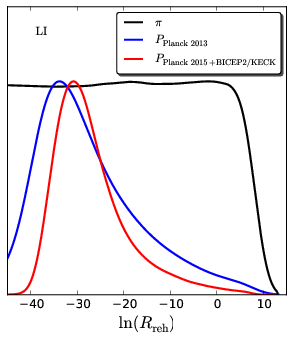
\includegraphics[width=0.45\linewidth, height=0.3\textheight]{Images/Chap3/Martin_Fig2A}
	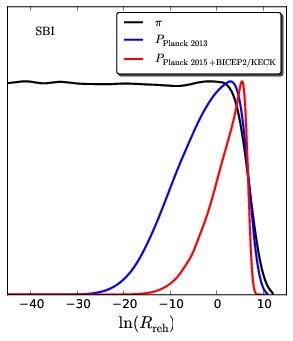
\includegraphics[width=0.45\linewidth, height=0.3\textheight]{Images/Chap3/Martin_Fig2B}
	\caption{Probability distributions (normalized to their maximum) for the rescaled reheating parameter $ R_{reh} $ associated with two of the 200 models analyzed: loop inflation on the left (LI) and supergravity brane inflation on the right (SBI) [\cite{Chap3:BraneInflation}]. The black curve corresponds to the prior (\ref{Chap3:PriorChoiche}) and is not exactly flat since the upper bound of (\ref{Chap3:PriorChoiche}) is slightly model dependent. The marginalized posterior obtained from  Planck 2013 data is displayed in blue and is to be compared to the more constraining posterior obtained from the Planck 2015 with BICEP/KECK (red curve) \cite{Chap3:Martin_Milestone}.}
	\label{fig:martinfig2a}
\end{figure}

The effective likelihood is defined as 
\begin{equation}
\label{Chap3:effectiveLikelihood}
\mathcal{L}_{eff}(P_{*},\epsilon_{i*}) \equiv \int P(D|\theta_{iac}, P_{*}, \epsilon_{i*})\pi(\theta_{iac})d\theta_{iac}.
\end{equation} 
Within a given slow-roll model of inflation $\mathcal{M}$, with theoretical parameters $\theta_{inf}$, the quantities $ P_{*} $ and $ \epsilon_{i*} $ are explicit function of $\theta_{inf}$ and, most importantly of $ \ln R_{reh} $. Thus, from Bayes' theorem, the posterior on $ \ln R_{reh} $ is given by
\begin{equation}
	P(\ln R_{reh}|D)= \frac{\pi(ln R_{reh})}{P(D|M)}
	\times \int \mathcal{L}[P_{*}(\theta_{inf},\ln R_{reh}), \epsilon_{i*}(\theta_{inf},\ln R_{reh})]\pi(\theta_{inf})d\theta_{inf},
\end{equation}
where $ P(D|M) $ is the global likelihood, which is proportional  to the Bayesian evidence $ P(\mathcal{M}|D)=P(D|\mathcal{M})\pi(\mathcal{M}) $ of the model $\mathcal{M}$ to explain the data D.

To fix better the idea in (Fig. \ref{fig:martinfig2a}) is reported the plot of \cite{Chap3:Martin_Milestone}, in which are represented the posteriors of $ \ln R_{reh} $ for two particular models: loop inflation and supergravity brane inflation using both the Planck 2013 and 2015 data. From the figure we can see the gain of information between these two data sets as well as the overall constraining power of CMB data on reheating. Of course, for other models $ \mathcal{M}_{i} $, the posteriors on $ \ln R_{reh} $ are different and may be peaked over large or small values, or not constrained at all.

We show in (Fig. \ref{fig:martinfig3a}) also the main plot of \cite{Chap3:Martin_Milestone}. In the plot each model is represented by a circle in the plane ($ \mathcal{B},D_{KL} $), where $\mathcal{B}$ is the Bayes' factor normalized to the best model, obtained from the global likelihoods by 
\begin{equation}
	\label{Chap3:BayesFactor}
	\mathcal{B} \equiv \frac{P(\mathcal{M}_{i}|D)}{sup_{j}[P(M_{j}|D)]}.
\end{equation}
Most of the models having large Bayes factor are concentrated around values $ D_{KL} \le 1 $, whereas disfavored models have $ D_{KL} > 2.5 $. This indicates how good a model fits the data. In the paper it is calculated also the average value of $ D_{KL} $ in the space of all models for Planck 2013 and Planck 2015 data, with 
\begin{equation}
<D_{KL}>\sum_{i} P(\mathcal{M}_{i}|D)D_{KL}(\mathcal{M}_{i}).
\end{equation}
This value is weighted by the Bayesian evidence, namely the probability of a model to explain the data. Disfavored models weight less than favored models. The authors estimate $ <D_{KL}> = 0.82 \pm 0.26 $ for Planck 2015 and  $ <D_{KL}> = 0.55 \pm 0.14 $. This leads a $ 40\% $ improvement in information gain from Planck 2015 compared to Planck 2013.

\begin{figure}[h]
	\centering
	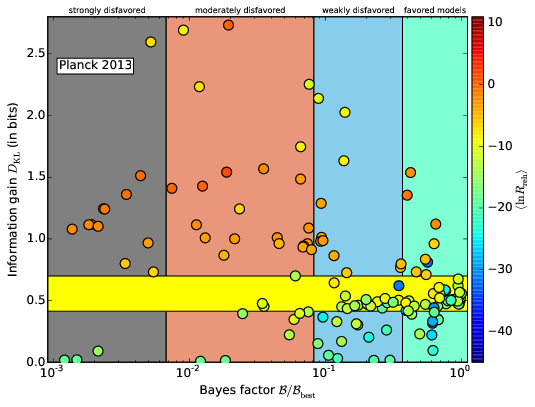
\includegraphics[width=0.75\linewidth, height=0.35\textheight]{Images/Chap3/Martin_Fig3A}
	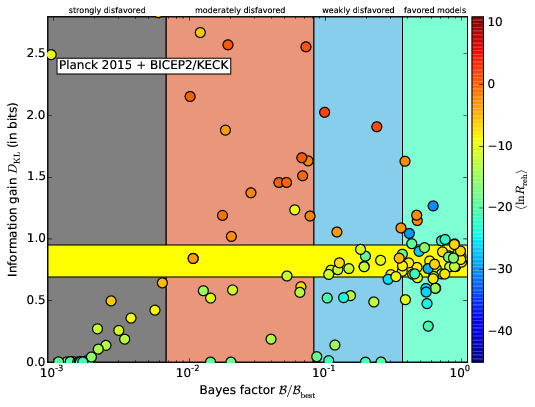
\includegraphics[width=0.75\linewidth, height=0.3\textheight]{Images/Chap3/Martin_Fig3B}
	\caption{Information gain $ D_{KL} $ in (bits) given by Planck 2013 (left panel) and Planck 2015 with BICEP2/KECK (right panel) about the rescaled reheating parameter $ \ln R_{reh} $ as a function of the Bayesian evidence. Each circle represents one of the 200 models of the \textit{Encyclopedia Inflationaris} collection whose color traces the mean value of $ \ln R_{reh} $. The yellow band represents the one-sigma deviation around the mean value. For Planck 2015 and BICEP2/KECK, one gets $ <D_{KL}> = 0.82 \pm 0.13 $. This corresponds to $ 40\% $ improvement compared to Planck 2013 \cite{Chap3:Martin_Milestone}. } 
	\label{fig:martinfig3a}
\end{figure}
\chapter{Preheating}
According to the theory of inflation, almost all elementary particles populating the universe are created during the reheating phase. In the previous chapters we introduced toy models of reheating that show the main idea. After inflation the inflaton oscillates near the minimum of its effective potential producing  particles that interact with each other and come to a state of thermal equilibrium at some reheating temperature $ T_{r} $. The process completes when all (or almost all) the energy of the classical scalar field $\phi$ transfers to the thermal energy of the  particles created in the process. 

A perturbative model of reheating is possible as long as the couplings are sufficiently small. However, the particle production from a coherently oscillating field for a wide range of couplings occurs in a non-perturbative regime of parametric excitation, called \textit{parametric resonance}. In fact, in a large part of inflationary models the first stages of reheating occur in a regime of a broad parametric resonance. This initial stage of reheating is called \textit{preheating}. A complete and analytical treatment of  preheating with parametric resonance after chaotic inflation  was introduced by Kofman, Linde and Starobinsky in \cite{Chap4:LindePreheatingModel}. During preheating the energy transfers from the inflaton field to other bose fields and particle production is extremely efficient. From the analysis in \cite{Chap4:LindePreheatingModel} comes out that reheating never completes at the stage of parametric resonance. Instead, the resonance becomes narrow and inefficient, and the final stages of  decay of the inflaton  can be described by a perturbative (elementary) theory of reheating. During preheating we have a copious particle production that occurs far away from thermal equilibrium. The energy of the inflaton zero mode is transferred to particles in an out-of-equilibrium state with very large occupation numbers within a very short time interval of about $ 10^{-35} $ seconds \cite{Chap7:Peloso_Thermalization}. One can expects that the initial conditions for the subsequent thermal history of the universe are settled during preheating. Moreover, a precise understanding of preheating and how thermal equilibrium is reached is crucial since partial thermal distributions can be responsible for cosmological baryo-leptogenesis, the possible creation of dangerous cosmological relics etc.

The most studied inflationary scenarios in which GW production is investigated during reheating are chaotic inflation and hybrid inflation. In the latter model preheating develops in a slightly different way compared to the first, with a mechanism called \textit{tachyonic preheating}. However, in both cases the process of gravitational waves production is essentially the same.

We start the discussion about preheating reviewing the Kofman-Linde-Starobinsky model in \cite{Chap4:LindePreheatingModel}. We will discuss the main points, see the paper for further details and references. For other references about preheating see \cite{Chap4:Lozanov}, \cite{Chap4:AminHetrzberg}, \cite{InflationDynamicsAndReheating:chap1}.

After preheating at the end of chaotic inflation scenario, we will discuss the tachyonic preheating after hybrid inflation and other important models discussed in the literature.

\section{Parametric Resonance Model}

\subsection{Elementary reheating}
We start considering a basic model that describes the interaction between the inflaton scalar field $\phi$ and a scalar field 	$\chi$ and a spinor field $\psi$:
\begin{equation}
	\label{Chap4:ElementaryReheating_Lagrangian}
	\mathcal{L}=\frac{1}{2}\partial_{\mu}\phi\partial^{\mu}{\phi} - V(\phi) +\frac{1}{2}\partial_{\mu}\chi\partial^{\mu}\chi -\frac{1}{2}m^{2}_{\chi}\chi^{2} + \bar{\psi}(i\gamma^{\mu}\partial_{\mu} - m_{\psi})\psi - \frac{1}{2}g^{2}\phi^{2}\chi^{2} - h\bar{\psi}\psi \phi,
\end{equation} 
where $ g,h $ are small coupling constants, and $ V(\phi) $ is the effective potential of the field $\phi$. 

During inflation the dynamics is leaded by the first two terms of the lagrangian. Consider the Klein-Gordon equation  for the inflaton field, $ \ddot{\phi} + 3H\dot{\phi} + V'(\phi) = 0 $. For sufficiently large initial value of the field, the friction term $ 3\dot{H}\phi $ dominates over $\ddot{\phi}$ and the potential term dominates over the kinetic term. In such a stage the universe expands quasi-exponentially. In the simplest model of chaotic inflation, $ V(\phi)=\frac{1}{2}m\phi^{2} $, inflation occurs at $\phi > M_{pl}$. With a decrease of the field $ \phi $ below $ M_{pl} $, the friction term becomes less and less important and inflation terminates at $ \phi \sim M_{pl}/2 $.

For the model (\ref{Chap4:ElementaryReheating_Lagrangian}) we consider first, for generality, the case in which the effective potential $ V(\phi) $ has a minimum at $ \phi = v $. Near the minimum the effective potential  is quadratic with respect to the field $\phi$, $ V(\phi) \sim \frac{1}{2}m^{2}(\phi-v)^{2} $, with $ m^{2} $ the effective mass squared of the inflaton field $\phi$. Suppose that we have a spontaneous symmetry breaking (SSB) of the parity symmetry $ \phi  \rightarrow -\phi$. In this case, we can expand the inflaton field around the minimum $ v $, $ \phi(x)=v + h(x)  $. Substituing this expansion in (\ref{Chap4:ElementaryReheating_Lagrangian}) and renaming $ h(x) $ with $\phi(x)$, the lagrangian becomes
\begin{equation}
	\label{Chap4:ElementaryReheating_LafterSSB}
	\mathcal{L}=\frac{1}{2}\partial_{\mu}\phi\partial^{\mu}\phi -\frac{1}{2}m^{2}\phi^{2} - \frac{1}{2}\partial_{\mu}\chi\partial^{\mu}\chi -\frac{1}{2}(m^{2}_{\chi} +g^{2}\sigma^{2})\chi^{2} + \bar{\psi}(i\gamma^{\mu}\partial_{\mu} - m_{\psi} - hv )\psi  - h\bar{\psi}\psi\phi -g^{2}v\phi\chi^{2}.
\end{equation}
After SSB we obtain then a correction for the effective mass of the field $\chi$, $ m^{2}_{\chi} \rightarrow m^{2}_{\chi}+g^{2}v^{2} $, a correction for the effective mass of $\psi$, $ m_{\psi} \rightarrow m_{\psi} + hv $, and a new term in the lagrangian, $ -g^{2}v\phi \chi^{2} $. Hereafter we rename $ m^{2}_{\chi} $ and $ m_{\psi} $ with the new effective masses after SSB. Moreover, we consider the case $ m \gg m_{\chi}, m_{\psi} $ with $ m_{\chi},m_{\psi} $ after the SSB, and we assume that after inflation $ H \ll m $. The last condition is always satisfied during the reheating stage.

The energy density of the oscillating inflaton field after the SSB is $ \rho_{\phi} = \frac{1}{2}\dot{\phi^{2}} + \frac{1}{2}m^{2}\phi^{2}$. Consider the field $\phi$ oscillating around $\phi=0$ with frequency $ k=m $. A homogeneous scalar field oscillating with frequency $ m $ can be considered as a coherent wave of $ \phi $-particles with zero momenta and with particle density $ n_{\phi}=\rho_{\phi}/m $. This means that $ n_{\phi} $ oscillators with the same frequency $ m $ that oscillate with the same phase can be described as a single homogeneous wave $\phi(t)$. If we consider time intervals larger than the typical oscillation time $ m^{-1} $, the energy density of the oscillating field $\rho_{\phi}$ and the number density of the particles $ n_{\phi} $ can be related to the amplitude of the inflaton $\Phi$, with $\rho_{\phi}=\frac{1}{2}m^{2}\Phi^{2}$ and $ n_{\phi}=\frac{1}{2}m\Phi^{2} $.

We consider now the effects related to the expansion of the universe and to particle production. The equation of motion for the inflaton field, considering a decay rate $ \Gamma $ and a Hubble constant $ H $, is
\begin{equation}
	\label{Chap4:ElemetaryReheating_EqMotion}
	\ddot{\phi} + (3H + \Gamma)\dot{\phi} + m^{2}\phi = 0.
\end{equation}
 In particular, the probability of decay of a $ \phi $-particle into a pair of scalar $ \chi $-particles or spinor $ \psi $-particles for $ m \gg m_{\chi},m_{\psi} $ is given by \cite{Chap4:LindePreheatingModel}
\begin{equation}
	\label{Chap4:ElemReheating_DecayRate}
	\Gamma(\phi \rightarrow \chi \chi) = \frac{g^{4}v^{2}}{8\pi m},
	\qquad
	\Gamma(\phi \rightarrow \psi \psi) = \frac{h^{2}m}{8\pi}.
\end{equation}
Solving the equation of motion (\ref{Chap4:ElemetaryReheating_EqMotion}), assuming $ H $ constant, we obtain the solution
\begin{equation}
	\label{Chap4:ElemReheating_solution}
	\phi(t)=\phi_{0}\exp\Big[-\frac{1}{2}(3H+\Gamma)t\Big]\sin(mt)=\Phi(t)\sin(mt).
\end{equation}
 This equation describes the damped oscillations of the field near $ \phi=0 $. This means that the amplitude of oscillations of the field $\phi$ decreases as $ \exp\Big[-\frac{1}{2}(3H+\Gamma)t\Big] $ due to particle production, which occurs during the decay of the inflaton field, and the expansion of the universe.

The decay products are ultrarelativistic ($ m \gg m_{\chi},m_{\psi} $). As seen in the previous chapters, reheating ends only when $ t $ becomes smaller than $\Gamma^{-1}$, because otherwise the main portion of energy remains stored in the inflaton field. Assuming that the universe reaches the thermodynamic equilibrium immediately after the complete decay of the field $ \phi $ at $ t \simeq \Gamma^{-1} $, we can estimate the reheating temperature as we did previously. 

However, this elementary theory has problems. First consider the fact that, in absence of fermions, the only contribution to the decay rate comes from $\Gamma(\phi \rightarrow \chi \chi) = g^{4}v^{2}/8\pi m $. This term vanishes in the theories without SSB, in which $ v=0 $. However, this doesn't mean that there is no reheating in theories without spontaneous symmetry breaking. In fact, we can have reheating also in the presence of a large oscillating field $\phi(t)$. We can obtain a naive estimate for the decay rate at $ v=0 $ writing $\Phi$ instead of $ v $ in the expression of the decay rate, obtaining $ \Gamma(\phi \phi \rightarrow \chi\chi) \simeq \frac{g^{4}\Phi^{2}}{8\pi m} $. In the chaotic inflation, for a quadratic potential, the beheaviour of the amplitude of the inflaton is $ \Phi^{2}\sim t^{-2} $, whereas the Hubble constant decreases as $ t^{-1} $. Thus, the decay rate never catches up with the expansion of the universe and reheating never completes. We can obtain a complete reheating only if $\Gamma$ decreases more slowly than $ t^{-1} $. An incomplete decay of the inflaton implies that the universe at the age of 10 billion years is cold, empty and unsuitable for life \cite{Chap4:LindePreheatingModel}. This could happens even if the coupling constant $ g^{2} $ is very large. Therefore, from the requirement that reheating has to complete we obtain important constraints on the theory.

The other problem with the elementary theory  is that it does not take into account  Bose condensation effects. Even if the couplings of the inflaton to bosons (for example $ \chi $) are small enough to allow for a perturbative coupling expansion, if many $\chi$-particles have been already produced and the phase space is densely populated, Bose condensation effects can greatly enhance the decay rate and lead to an explosive production of particles. Moreover, for larger couplings the perturbative methods fail and  particle production then must be treated as a non-perturbative effect. 

The inflaton condensate is a coherent oscillating homogeneous field. This means that particle production has to be treated as a collective process in which many inflaton particles decay simultaneously, not independently of each other. Moreover, due to the large occupation number we can treat the condensate classically.

 We see now that the periodic time-dependence of the effective masses of the decay products in the classical oscillating background can have a powerful effect on their production rates in the form of the parametric resonance.
\subsection{Parametric resonance}
Consider the interaction between the classical inflaton field $\phi$ and the quantum scalar field $\hat{\chi}$ with lagrangian given by (\ref{Chap4:ElementaryReheating_Lagrangian}). We can represent the quantum field $\hat{\chi}$ as 
\begin{equation}
	\label{Chap4:RepresentationScalarField}
	\hat{\chi}(t,\textbf{x}) = \frac{1}{(2\pi)^{3/2}}\int d^{3}k \Bigg(\hat{a}_{k} \chi_{k}(t)e^{-i\textbf{k}\cdot\textbf{x}} + \hat{a}^{+}_{k} \chi_{k}^{*}(t)e^{i\textbf{k}\cdot\textbf{x}}\Bigg),
\end{equation}
where $ \hat{a}_{k} $ and $ \hat{a}^{+}_{k} $ are the annihilation and creation operators. Now, the equation of motion for $\chi_{k}$, $ \frac{\delta S}{\delta \chi_{k}}=0 $, reads
\begin{equation}
	\label{Chap4:elemReheating_eomChi1}
	\Box \chi = \frac{\partial V(\phi,\chi)}{\partial \chi},
\end{equation}
where $\Box$ is the covariant D'alembert operator, given by (\ref{alembertOperator}). From the lagrangian (\ref{Chap4:ElementaryReheating_Lagrangian}) the equation of motion becomes
\begin{equation}
	\label{Chap4:elemReheating_eomChi}
	\ddot{\chi_{k}} + 3\frac{\dot{a}}{a}\dot{\chi_{k}} + \Bigg(\frac{\textbf{k}}{a^{2}} + \bar{m}^{2}_{\chi} + g^{2}\phi^{2}\Bigg)\chi_{k}=0.
\end{equation}
This equation describes an oscillator with a variable frequency $\omega(t)$ due to the changing with time of the scale factor $ a(t) $ and the background field $ \phi(t) $. We suppose that the effective mass $ \bar{m}_{\chi} + g^{2}\phi^{2} $ vanishes for $ \phi=0 $, i.e. $  \bar{m}_{\chi}=0 $.

Consider the potential that reproduces the SSB, $ V(\phi) \sim \frac{1}{2} m^{2} (\phi - v)^{2} $.  After the SSB the lagrangian (\ref{Chap4:ElementaryReheating_Lagrangian}), considering only the scalar sector, reads
\begin{equation}
\label{Chap4:ParamResonanceLagrangian}
\mathcal{L}=\frac{1}{2}\partial_{\mu}\phi\partial^{\mu}\phi -\frac{1}{2}m^{2}\phi^{2}+ \frac{1}{2}\partial_{\mu} \chi \partial^{\mu}\chi-\frac{1}{2}g^{2}v^{2}\chi^{2} - \frac{1}{2}g^{2}\phi^{2}\chi^{2}-g^{2}v\phi\chi^{2}.
\end{equation}  
Assume that the amplitude of $\phi$-oscillations are much smaller than $ v $, and neglect for the moment the expansion of the universe (set $ a=1 $). The equation for the modes (quantum fluctuations) of the field $\chi$ with physical momentum \textbf{k} (\ref{Chap4:elemReheating_eomChi}) becomes
\begin{equation}
	\label{Chap4:ParamResonance_eqMotion}
	\ddot{\chi_{k}} + (k^{2} + g^{2}v^{2} + 2g^{2}v \Phi \sin mt)\chi_{k} = 0,
\end{equation}
where $ k=\sqrt{\textbf{k}^{2}} $, and $\Phi$ stands for the amplitude of oscillations of the inflaton field. This equation describes an oscillator with a periodically changing frequency $ \omega^{2}(t) = k^{2} + g^{2}v^{2} + 2g^{2}v\Phi \sin mt $. For certain values of $ k $ this periodicity may lead parametric resonance. To see this effect we have to cast (\ref{Chap4:ParamResonance_eqMotion}) in the well known Mathieu equation. First, make the change of variables in $ mt=2z-\pi/2 $. In this way $ \sin (2z-\pi/2)=-cos (2z)  $. With this change of variable, the equation (\ref{Chap4:ParamResonance_eqMotion}) becomes
\begin{equation}
\label{Chap4:ParamResonance_eqMotion2}
\chi_{k}'' + \Bigg(4\frac{k^{2} + g^{2}v^{2}}{m^{2}}-\frac{8g^{2}v\Phi}{m^{2}} \cos(2z)\Bigg)\chi_{k} = 0,
\end{equation}
where prime denotes differentiation with respect to $ z $.
  Setting $ A_{k}=4\frac{k^{2} + g^{2}v^{2}}{m^{2}},\  q=\frac{4g^{2}v\Phi}{m^{2}} $ and $ z=\frac{mt}{2} $, we finally obtain the Mathieu equation:
\begin{equation}
	\label{Chap4:ParamResonance_MathieuEquation}
	\chi_{k}''+(A_{k} - 2q\cos(2z))\chi_{k}=0.
\end{equation}

The Mathieu equation is a type of Hill's equation
\begin{equation}
	\label{Chap4:Mathieu_HillEquation}
	\ddot{u_{k}} + \omega^{2}(k,t)u_{k}(t) = 0,
\end{equation}
where the angular frequency is periodic, $ \omega^{2}(k,t)=\omega^{2}(k,t+T) $.
From the Floquet theorem the most general solution of the Hill's equations is given by
\begin{equation}
\label{Chap4:solutionHillEquation}
u_{k}(t) = e^{\mu_{k}t}\mathcal{P}_{k+}(t) + e^{-\mu_{k}t}\mathcal{P_{k-}}(t),
\end{equation}
where $\mu_{k}$ is called Floquet exponent and $\mathcal{P}_{k}(t)=\mathcal{P}(t+T)$ is a periodic function. If the real part of the Floquet exponent $\mathcal{R}(u_{k}) $ is different from zero, one of the two terms increases exponentially with time. This is what we call parametric resonance. We can easily prove (\ref{Chap4:solutionHillEquation}).

First, we can put the Hill's equation (\ref{Chap4:Mathieu_HillEquation}) in the form
\begin{equation}
	\frac{d}{dt}
\left(
\begin{array}{c}
	u_{k}(t) \\
	\dot{u}_{k}(t)	
\end{array}
\right)
=
\left(
\begin{array}{cc}
	0  & 0 \\
	\omega^{2}(t) & 0
\end{array}
\right)
\left(
\begin{array}{c}
	u_{k}(t) \\
	\dot{u}_{k}(t)	
\end{array}
\right),
\end{equation}
and, more compactly,
\begin{equation}
	\label{Chap4:CompactHillEquation}
	\frac{d}{dt} x(t) = A(t) x(t),
\end{equation}
with $ x(t)=(u_{k}(t),\dot{u}_{k}(t))^{T} $, and $ A(t)=A(t+T) $. From (\ref{Chap4:CompactHillEquation}) we can easily see that if $ x(t) $ solves this equation, also $ x(t+T) $ is a solution. Obviously, the same is valid also for $ u_{k}(t) $. Consider now two independent solutions of (\ref{Chap4:Mathieu_HillEquation}), $ u_{k1}(t) $ and $ u_{k2}(t) $. If they are solutions, then also a general linear combination of them is a solution at the time $ t $ and at $ t+T $. Moreover, we can express them, evaluated at $ t+T $, in terms of $ u_{k}(t) $ evaluated at time $ t $, i.e. $ u_{k1}(t+T)=B_{11}u_{k1}(t) + B_{12}u_{k2}(t) $ and $ u_{k2}(t+T)=B_{21}u_{k1}(t) + B_{22}u_{k2}(t) $. We can rewrite this in a more compact way, $ u_{ki}(t+T)= \sum_{j=1}^{2}B_{ij}u_{kj}(t) $ with $ B_{ij} $ a constant $ 2\times 2 $ invertible matix. Diagonalizing the last equation, we obtain $ v_{ki}(t+T)=\sum_{j=1}^{2}\lambda_{i}^{B}\delta_{ij}v_{kj}(t) $, where $ \lambda_{i}^{B} $ are two eigenvalues of $ B_{ij} $ and $ v_{ki}(t) $ are independent linear combinations of $ u_{ki}(t) $. Then, we obtain that with a time shift $ t \rightarrow t+T $ we have a rescaling by an eigenvalue, $ v_{ki}(t+T)=\lambda_{i}^{B}v_{ki}(t) $. 
The most general solutions with this property are $ v_{ki}(t)=(\lambda_{i}^{B})^{t/T}P_{ki}(t) $, where $ P_{ki}(t+T)=P_{ki}(t) $. \\ Now, the Wronskian of the Hill's equation (\ref{Chap4:Mathieu_HillEquation}) is given by $ W[u_{k1},u_{k2}]=u_{k1}\dot{u}_{k2}-\dot{u}_{k1}u_{k2} $. Deriving the Wronskian and using the Hill's equation (\ref{Chap4:Mathieu_HillEquation}), we obtain $ \dot{W}[u_{k1},u_{k2}]=0 $. So must be $ \dot{W}[v_{k1},v_{k2}]=0$. On the other hand, it is easy to see that $ W[v_{k1},v_{k2}](t+T) = \lambda_{1}^{B}\lambda_{2}^{B}W[v_{k1},v_{k2}](t) $. This means that $ \lambda_{1}^{B}=1/\lambda^{B}_{2} \equiv \lambda^{B} $. The Floquet exponent is simply $ \mu_{k} = \ln(\lambda^{B})/T $, and in (\ref{Chap4:solutionHillEquation}) $\mathcal{P}_{k\pm}(t)$ is some linear combination of $ P_{k1,2}(t) $ \cite{Chap4:AminHetrzberg}, \cite{Chap4:Lozanov}.\

To find the Floquet exponent we  just need to calculate the eigenvalues of $ B_{ij} $. From \cite{Chap4:Lozanov} we point out a consideration. Consider the initial conditions $ u_{k1}(t_{0}) = 1 $, $ \dot{u}_{k1}(t_{0})=0 $ and $ u_{k2}(t_{0}) = 1 $, $ \dot{u}_{k2}(t_{0})=0 $. After evolving the Hill's equation for one period $ T $ for the two sets of initial conditions, the eigenvalues found in \cite{Chap4:Lozanov} are 
\begin{equation}
\lambda_{1,2}^{B}=\frac{1}{2}\Bigg[u_{k1}(t_{0} + T) + \dot{u}_{k2}(t_{0} + T)  \pm \sqrt{[u_{k1}(t_{0} + T) - \dot{u}_{k2}(t_{0} + T)]^{2} + 4\dot{u}_{k1}(t_{0}+T)u_{k2}(t_{0} + T)}\Bigg].
\end{equation}
We see that the initial conditions are relevant for the efficiency of the parametric resonance. If both the initial field and field velocities are zero, parametric resonance does not lead any growth. Therefore we obtain a difference respect to the case of ordinary resonance. In the ordinary resonance the forcing term leads to a rapid growth even if the field displacement and velocity are zero. Instead, in the parametric resonance we have no resonant excitations if no energy is stored in the fluctuations initially. This is the reason why vacuum fluctuations, even if small, are crucial for the particle production during preheating.

\begin{figure}
	\centering
	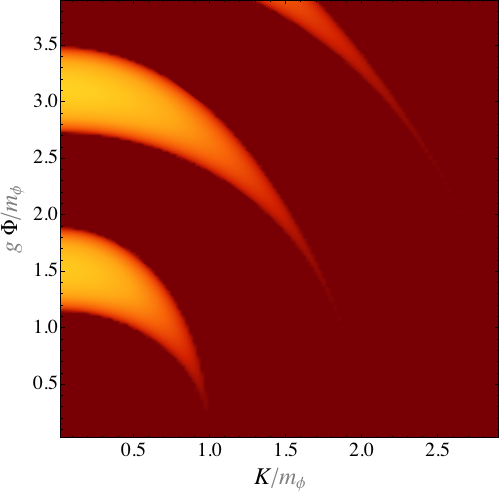
\includegraphics[width=0.6\linewidth, height=0.4\textheight]{Images/Chap4/AminHertzberg_MathieuChart}
	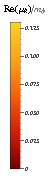
\includegraphics[width=0.15\linewidth, height=0.4\textheight]{Images/Chap4/MathieuChart_Legend}	
	\caption{A plot of the instability band structure for the model $ V(\phi, \chi)=\frac{1}{2}m^{2}_{\phi}\phi^{2} + \frac{1}{2}m^{2}_{\chi_{_{_{}}}}\chi^{2} + \frac{1}{2}g^{2}\phi^{2}\chi^{2} $. The color represents the real part of the Floquet exponent rescaled by the mass of the inflaton, $ \mathcal{R}(\mu_{k})/m_{\phi} $. The two other axes represent the scaled amplitude of the inflaton field, $ g\Phi/m_{\phi} $, and the rescaled wavenumber $ K/m_{\phi} $, where $ K=\sqrt{k^{2} + m^{2}_{\chi}} $ \cite{Chap4:AminHetrzberg}.}
	\label{fig:mathieuchartlegend}
\end{figure}
The properties of the solution of the Mathieu equation are represented by the stability/instability chart, plotted in (Fig. \ref{fig:mathieuchartlegend}) from \cite{Chap4:AminHetrzberg}. There is a region of stability, the dark-red zone, in which $\mathcal{R}(\mu_{k})=0$. The lighter regions are the  unstable zones in which $\mathcal{R}(\mu_{k})>0$. 

However, for now consider the case in which $ |q|\ll 1 $ and $ A_{k}> 0$. The regions of instability become narrow and approach $ A_{k}^{(n)}\simeq n^{2} $ as $ q\rightarrow 0 $ ($ n  $ integer). In the first narrow band the peak value of the Floquet exponent is $ \mathcal{R}(\mu_{k}) \simeq |q|/2 $, while $ A_{k}^{(1)} \simeq 1 \pm |q| = 1 \pm \frac{4g^{2}v\Phi}{m^{2}} $ \cite{Chap4:Mechanics}. In this case  the first band is the widest and most important band. The Floquet exponent $\mu_{k}$ describes the rate of the exponential growth and in the first band, for $ m^{2} \gg g^{2}v^{2} $, is given by \cite{Chap4:LindePreheatingModel}
\begin{equation}
	\label{Chap4:FloquetExponent}
	\mu_{k}=\sqrt{\Bigg(\frac{q}{2}\Bigg)^{2} - \Bigg(\frac{2k}{m}-1\Bigg)^{2}}.
\end{equation}
Considering the condition to have resonance, $\mathcal{R}(\mu_{k}) \neq 0$, the resonance occurs for $ k=\frac{m}{2}(1 \pm \frac{q}{2}) $. The maximal value is reached at $\mu_{k}=\frac{q}{2}=\frac{2g^{2}v\Phi}{m^{2}}$ at $ k=m/2 $, and the corresponding modes $ \chi_{k} $ grow at a maximal rate $ \exp(qz/2)=\exp(\frac{qmt}{4})=\exp(\frac{g^{2}v\Phi t}{m}) $. 

With the growth of the modes $ \chi_{k} $, we have a growth of the occupation number of the created particles $ n_{k}(t) $. In fact, we can estimate the number density $ n_{k} $ of particles with momentum $ \textbf{k} $ as the energy of the mode $ \frac{1}{2}|\dot{\chi}_{k}|^{2} + \frac{1}{2}\omega_{k}^{2}|\chi_{k}|^{2} $ divided by the energy $ \omega_{k} $ for each particle:
\begin{equation}
n_{k}=\frac{\omega_{k}}{2}\Bigg(\frac{|\dot{\chi_{k}}|^{2}}{\omega_{k}^{2}} + |\chi_{k}|^{2}\Bigg) - \frac{1}{2}.
\end{equation}
When the modes $ \chi_{k} $ grow as  $\exp(qz/2) $, the number of $ \chi $-particles grows as $ \exp(qz)= \exp(\frac{2g^{2}v\Phi t}{m}) $.

Since the resonance occurs near $ k=m/2 $, we can interpret this process as a decay of a $ \phi $-particle in two $ \chi $-particles with momentum $\sim k/2$.
In the perturbative limit the tree-level order Feynman diagrams gives the dominant contribution to the decay of the inflaton condensate into $ \chi $-particles. Feynman diagrams of higher order describe the simultaneous decay of more than one inflaton particles from the condensate and are negligible in the perturbative limit.
The main difference between  perturbation theory and parametric resonance is that in the first model the amount of produced particles does not depend on the number of particles produced earlier. Indeed, considering the rate of production $ \Gamma(\phi \rightarrow \chi \chi) = \frac{g^{4}v^{2}}{8\pi m} $, the decay rate $ \Gamma^{-1} $ is suppressed by the factor $ g^{4} $ making the decay very slow in the weak coupling limit. Instead, in parametric resonance the rate of the process can be calculated as $ u_{k}m \sim \frac{g^{2} v \Phi}{m} $, which is greater than $\Gamma$ for $ \Phi > \frac{g^{2}v}{8\pi} $, and the rate of production of $ \chi $-particles is proportional to the amount of particles produced earlier (this is the reason why we have an exponential growth). However, even if the elementary theory and preheating due to parametric resonance are two completely different effects, these processes may coexist. Moreover, parametric resonance in the narrow resonance regime  $ |q| \ll 1 $ is in good agreement with the perturbative treatment of Bose condensation \cite{Chap4:Lozanov}.

Thus, we have this picture. In the beginning the inflaton field $\phi$ oscillates with amplitude $ \Phi > \frac{g^{2} v}{8\pi} $ and we have parametric resonance with an exponential growth of the modes $\chi_{k}$. However, the inflaton loses its energy with the time and the amplitude becomes smaller than $ \frac{g^{2}v}{8\pi} $. From this point, the amplitude of the field $ \Phi $ decays exponentially within a time $ \Gamma^{-1} $, which is smaller than the typical time necessary for parametric resonance to occur. 

During the expansion of the universe the field $\phi$ decreases also for the friction term $ 3H\dot{\phi} $ in the equation of motion for the field $\phi$. Then we should compare $ qm $ with the effective decay rate $ 3H + \Gamma $. Parametric resonance occurs for $ qm > 3H + \Gamma $. Considering that the perturbative decay is inefficient at $ \Gamma < H $, we can consider only the condition $ qm > 3H $.

Parametric resonance can become inefficient also if the  momenta $ k $ are redshifted away from the resonance band. If the total width of the first band is given by $ qm $, we consider the part in which the resonance is efficient as $ qm/2 $. We can then roughly estimate the time in which a given mode remains within this band as $ q/H $, and depends on the equation of state of matter. During this time the number of particles in growing modes increases as $ \exp(\frac{q^{2}m}{2H}) $. This implies that we obtain an efficient decay of the inflaton field only if $ q^{2}m \ge H $ (see \cite{Chap4:LindePreheatingModel}). 

In the model considered the two conditions for an efficient resonance, $ qm \ge \Gamma $ and $ q^{2}m \ge H $, yield for the amplitude of the inflaton field the constraints
\begin{equation}
\label{Chap4:conditionAmplitudeField}
\Phi \ge \frac{g^{2}}{32\pi}v, \qquad  \Phi \ge \frac{m\sqrt{mH}}{4g^{2}v}.
\end{equation}
From this model we obtain that parametric resonance can be efficient only at a sufficiently large  amplitude $\Phi$, but reheating never ends in the regime of parametric resonance. Instead, as soon as the amplitude of oscillations becomes sufficiently  small, parametric resonance terminates and reheating can be described by the elementary theory.

In this simple model with SSB $ (v \neq 0) $ we assumed that the amplitude of oscillations of the inflaton field is very small, i.e $ \Phi \ll v $, and we considered only the quadratic part of the effective potential $ V(\phi) \sim (\phi - v)^{2} $. However, considering a realistic model of SSB this condition is satisfied only at the end of parametric resonance. Therefore, instead of this model, we can consider a model with spontaneous symmetry breaking with the potential $ V(\phi)=\frac{\lambda}{4}(\phi^{2}-v^{2})^{2} $, with $ m \gg m_{\chi},\ \lambda \gg g^{2} $. Unlike the previous model, in this case the interaction term $\frac{\lambda}{4}\phi^{4}  $ becomes more important than $ g^{2}\phi^{2}\chi^{2} $. This leads to a more efficient production of $ \phi $-particles respect to the production of $ \chi $-particles.

Assume that in the beginning the inflaton field $ \phi $ is at the top of the potential at $ \phi=0 $. In this case we have a negative effective mass squared. This implies, independent of any parametric resonance, a production of particles through a tachyonic process. However, this effect does not last long because away from the maximum the curvature of the potential becomes positive. When $ \phi = v $, the inflaton field begins to oscillate near its minimum. In this case the parametric resonance  with $ \phi $-particle production can be represented with a Mathieu equation  for the fluctuations $\delta \phi_{k}$. 
The decay of the coherently oscillating inflaton field $\phi$ into $\phi$-particles remains the dominant process until the amplitude of the field $\Phi$ becomes much smaller than $ v $, after which the decay $ \phi \rightarrow \chi \chi $ becomes more important. In the end, when the amplitude of the oscillations $ \Phi $ becomes smaller than $ \frac{g^{2}}{32\pi}v $  or   $ \frac{m\sqrt{mH}}{4g^{2}v} $, the parametric resonance stops and the decay $ \phi \rightarrow \chi \chi $ is described by the elementary reheating.
In this theory the process of $ \chi $-particle production is more efficient than $\phi$-particle production only for $ \Phi \ll v $.

The models studied in this section are a good laboratory to study different features of parametric resonance. However, there is a problem with the initial conditions. There is no a valid reason why the inflaton field should be stay initially at the top of the potential at $ \phi=0 $. Also, the shape of the potential is rather artificial. For this reason, from the next section we move in the more realistic scenario of chaotic inflation. In this theory, with a simple potential $ \frac{1}{2}m^{2}\phi^{2} $, the parametric resonance becomes very different.
 \section{Resonance after Chaotic Inflation}
 In the chaotic inflation we don't  impose any initial condition on the initial value of the inflaton. The amplitude  of oscillations of the inflaton can be as large as $ M_{pl} $, i.e. much greater than any other parameters such as $ v $. We consider now the lagrangian (without SSB)
 \begin{equation}
 	\label{Chap4:potentialChaoticInflation}
 	\mathcal{L}=\frac{1}{2}\partial_{\mu}\phi\partial^{\mu}\phi + \frac{1}{2}\partial_{\mu}\chi\partial^{\mu}\chi - \frac{1}{2}m^{2}\phi^{2} - \frac{1}{2}g^{2}\phi^{2}\chi^{2},
 \end{equation}
from which the equation for the fluctuations $ \chi_{k} $ is
 \begin{equation}
 	\label{Chap4:eqFluctuationChaoticModel}
 	\ddot{\chi_{k}} + (k^{2} + g^{2}\Phi^{2}\sin^{2}(mt))\chi_{k}=0.
 \end{equation}
From this, putting $ z=mt $, we can derive the Mathieu equation 
\begin{equation}
	\label{Chap4:eqMotionChi}
	\chi_{k}'' + (A_{k} - 2q\cos(2z))\chi_{k}=0,
\end{equation}
where, in this case, $ q=\frac{g^{2}\Phi^{2}}{4m^{2}} $,  $ A_{k} = \frac{k^{2}}{m^{2}} + 2q  $ and $ z=mt $. For $ g\Phi < m $ we have  narrow resonance with $ q \ll 1 $. Considering the first band $ A_{k}^{(1)}\simeq 1\pm q \simeq \frac{k^{2}}{m^{2}} + 2q $, the resonance is obtained for the modes $ k^{2}\sim m^{2}(1-2q \pm q) $. The modes $\chi_{k}$ with momenta corresponding  to the center of resonance at $ k \sim m $ grow as $\exp(\mu_{k}z)\simeq \exp(qz/2)\sim \exp(\frac{g^{2}\Phi^{2}t}{8m})$. At the same time, the number of $\chi$-particles grows as $\exp(2\mu_{k}z) \simeq\exp(qz) \sim \exp(\frac{g^{2}\Phi^{2}t}{4m})$. We can interpret this process as a resonance with decay of two $ \phi $-particles with mass $ m $ to two $\chi$-particles with momenta $ k\sim m $.

However, for oscillations with a large amplitude $\Phi$, the parameter $ q $ can be very large. In this case the resonance occurs for a broad range of values $ k $ and reheating becomes extremelly efficient. Considering the stability/instability chart for the Mathieu equation, the resonance occurs for modes  with $ \frac{k^{2}}{m^{2}}=A-2q $, i.e. above the line $ A=2q $. In this regime we can't apply the standard methods of the narrow resonance.

This broad resonance regime becomes important when we take into account the expansion of the universe. In the previous section we have seen that resonance in an expanding universe occurs only if $ q^{2}m \ge H $. This implies
\begin{equation}
	\label{Chap4:ConditionExpansionUniverse}
	g\Phi \ge 2m\Bigg(\frac{H}{m}\Bigg)^{1/4}.
\end{equation}
In the simplest inflationary models the value of the Hubble constant at the end of inflation is of the same order of the inflaton mass $ m $, $ H \sim m $. We can then conclude that the regime of the resonance reheating occurs only if the amplitude of the inflaton oscillations satisfies the condition $ \Phi > m/g $. The resonance stops at $ \Phi < m/g $ when $ q \le 1/4 $. Therefore, preheating in this model cannot begin for $ \Phi < m/g $. In fact, efficient preheating requires extremely large initial values of $ q $. The reason is that the amplitude of the inflaton field decreases rapidly during the expansion of the universe. Thus, for not very large initial values of $ q $, the condition (\ref{Chap4:ConditionExpansionUniverse}) becomes violated before the resonance has enough time to transfer the energy from the oscillating inflaton field into the energy of $ \chi $-particles. In this model preheating is efficient only if the initial value of $ q $ at the end of inflation is very large, $ q_{0} \ge 10^{3} $.

For this huge value of $ q $, the expansion of the universe makes preheating very peculiar and, instead of regular resonance, we obtain a  \textit{stochastic resonance} (Fig \ref{fig:lindefig4} from \cite{Chap4:LindePreheatingModel}).
\begin{figure}
	\centering
	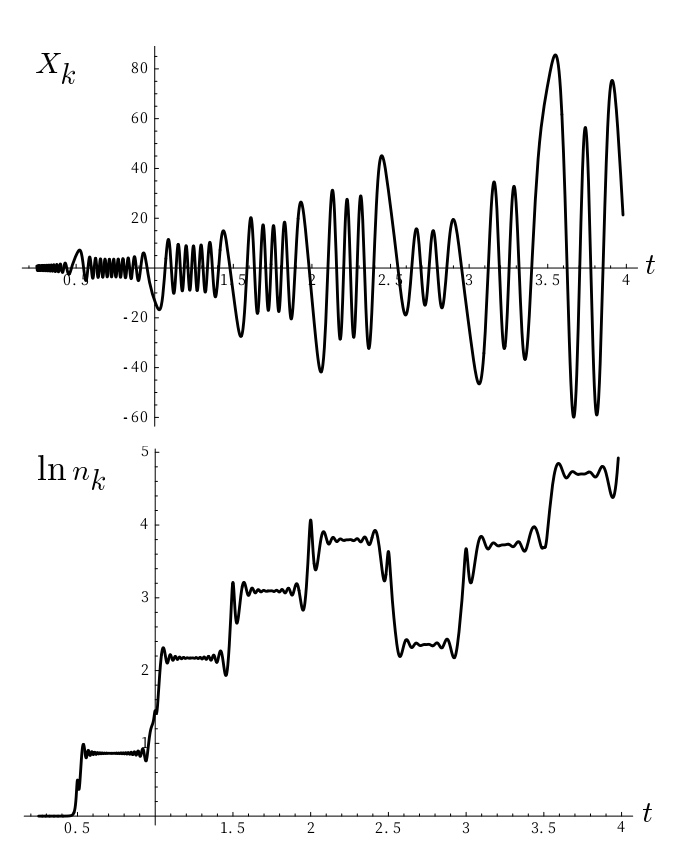
\includegraphics[width=0.6\linewidth, height=0.4\textheight]{Images/Chap4/Linde_Fig4}
	\caption{Parametric resonance in the theory $ m^{2}\phi^{2} $ in an expanding universe with scale factor $ a\sim t^{2/3}$ for $g=5\times 10^{-4} $ and $ m=10^{-6} M_{pl} $. The initial value of $ q $ in this process is $ q_{0}\sim 3 \times 10^{3} $.	The number of particles  $ n_{k} $ in this process typically increases, but it may occasionally decrease as well. This is a distinctive feature of stochastic resonance in an expanding universe. A decrease in the number of particles is a purely quantum mechanical effect which would be impossible if these particles were in a state of thermal equilibrium \cite{Chap4:LindePreheatingModel}.}
	\label{fig:lindefig4}
\end{figure}


\subsection{Stochastic resonance}
Consider the fluctuations $\chi_{k}$ in an expanding universe with $ m^{2}_{\chi}=0 $ and, after inflation, in a matter-dominated like era with $ a(t)=(t/t_{0})^{2/3} $. We consider $ t_{0} $ as initial time, counted from the end of inflation. 
With these assumptions, for sufficiently large $ t $, we can write the solution for the inflaton field after inflation as 
\begin{equation}
\label{Chap4:solutionInflaton}
\phi(t)=\Phi(t)\ \sin(mt),
\qquad
\Phi(t) = \frac{M_{pl}}{\sqrt{3\pi}mt}.
\end{equation}
We can simplify the study of the parametric resonance stage in the expanding universe introducing the function $ X_{k}(t)=a(t)^{3/2}\chi_{k}(t) $ (that it is equal to $ \frac{t}{t_{0}}\chi_{k}(t) $ in this case). The equation for the fluctuations $ \chi_{k} $ (\ref{Chap4:elemReheating_eomChi}) becomes simply
\begin{equation}
	\label{Chap4:ChaoticInflation_CompactEquationChi}
	\ddot{\chi_{k}} + \omega_{k}^{2}X_{k} = 0,
\end{equation}
where 
\begin{equation}
	\label{Chap4:ChaoticInflation_Omega_k}
	\omega_{k}^{2}=\frac{k^{2}}{a^{2}(t)} + g^{2}\Phi^{2}\sin^{2}(mt) + \Delta,
\end{equation}
with $ \Delta=m_{\chi}^{2}-\frac{3}{4}(\frac{\dot{a}}{a})^{2}-\frac{3}{2}\frac{\ddot{a}}{a} $. This term is usually very small. Indeed, we are considering the case in which $ m_{\chi}\simeq 0 $. Moreover,  soon after the end of inflation $ H^{2}=(\frac{\dot{a}}{a})^{2}\sim \frac{\ddot{a}}{a} \ll m^{2} $. Then, we can neglect this term. This equation describes an oscillator with a variable frequency $ \omega_{k}^{2}(t) $ due to the time-dependence of the background field $\phi(t)$ and $ a(t) $. The initial condition is given by the positive-frequency solution, $ X_{k}(t) \simeq e^{-\omega_{k}t}/\sqrt{2\omega_{k}} $.

We consider now the comoving occupation number of particles $ n_{k} $ in the mode $ k $ in an expanding universe,
\begin{equation}
	\label{Chap4:comovNumberParticles}
	n_{k}=\frac{\omega_{k}}{2}\Bigg(\frac{|\dot{\chi}_{k}|^{2}}{\omega^{2}_{k}} + |\chi_{k}|^{2}\Bigg) - \frac{1}{2}.
\end{equation}
This quantity is an adiabiatic invariant of (\ref{Chap4:ChaoticInflation_CompactEquationChi}). Indeed, in the WKB approximation, i.e. $\dot{\omega} \ll \omega^{2}$, the comoving number of particles $ n_{k} $ does not change with time. This is not true when the adiabatic approximation (and then the condition $\dot{\omega} \ll \omega^{2}$ ) is violated. The violent production of particles occurs, indeed, when the adiabatic approximation is broken.

We can study the beheaviour of $ X_{k} $ and $ n_{k} $ from the following consideration. The number of bands in the theory of Mathieu equation is given by $ n=\sqrt{A} $. In this model reheating occurs for $ A\sim 2q $, that implies $ n\sim\sqrt{2q}\sim g\Phi/m $. In the numerical analysis in \cite{Chap4:LindePreheatingModel}, with $ m\sim 10^{-6} M_{pl} $ and $ g\sim 10^{-1} $, from the first oscillation to the second oscillation the band number decreases from $ n \sim 3 \times 10^{3} $ to $ n\sim 1.5 \times 10^{3} $, because the amplitude $\Phi$ drops by a factor two after the second oscillation. Therefore, during a single oscillation of the inflaton the field does not remain in the same instability band of the Mathieu equation, but it jumps over $ 10^{3} $ different instability bands. Thus the standard approaches to study the Mathieu equation completely fails here.

However, as we will see in the next subsection, in the broad resonance regime particle production occurs only in a small interval around $ \phi=0 $. Nothing depends on the exact way the inflaton field $\phi$ beheaves in other moments. This happens because the WKB approximation breaks when the field $ \phi(t)=0 $. Then, the comoving number of particles $ n_{k} $  is not anymore an adiabatic conserved quantity, i.e. it changes with time. 

\begin{figure}
	\centering
	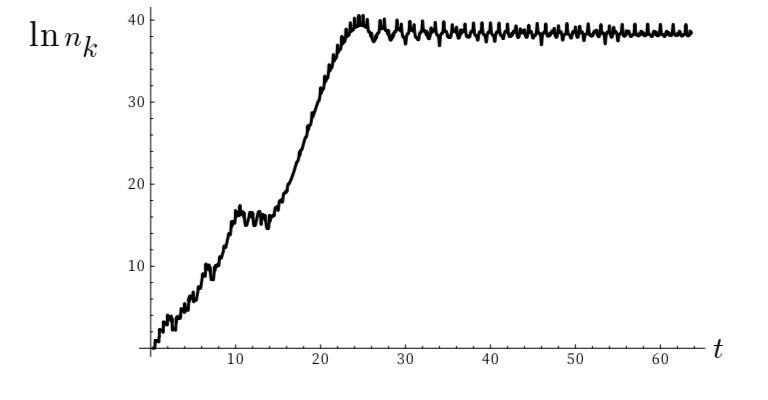
\includegraphics[width=0.7\linewidth, height=0.3\textheight]{Images/Chap4/Linde_Fig6}
	\caption{Parametric resonance in the theory $ m^{2}\phi^{2} $ in an expanding universe with scale factor $ a\sim t^{2/3}$ for $g=5\times 10^{-4} $ and $ m=10^{-6} M_{pl} $. Towards the end of this period, after approximatevely 25 oscillations of the inflaton field, the resonance ceases to exist, and the occupation number $ n_{k} $ becomes constant \cite{Chap4:LindePreheatingModel}.}
	\label{fig:lindefig6}
\end{figure}
Therefore, we have the following picture. Stochastic resonance occurs only in the first part of the process, when the value of  $ q $ is very large and the resonance is very broad.  During this phase particles are produced in bursts near the moment when $ \phi(t)=0 $, raher than smoothly as in the narrow resonance regime. Gradually, the amplitude of the field $\phi$ decreases, which makes $ q $ smaller. The field then stays in each resonance band for a longer time, also because the expansion of the universe slows down. The stochastic regime ends and the regular resonance begins when the parameter $ q $ drops from $ q \gg 1 $ to $ q \sim 1 $.

 The numerical analysis in \cite{Chap4:LindePreheatingModel} provides the following beheaviour. The transition from the stochastic resonance to a regular one is shown as a short plateau for $ \ln n_{k} $ in the plots of \cite{Chap4:LindePreheatingModel} (Fig. \ref{fig:lindefig6} from \cite{Chap4:LindePreheatingModel}). During this short stage the resonance is no longer stochastic and the mode $ X_{k} $ appears in the region of stability, which divides the second and the first instability band of the Mathieu equation. After this little time of stability, we don't have a broad resonance anymore, but the amplitude still grows exponentially at high rate until the amplitude of the field $ \Phi $ becomes smaller than $ m/g $, which corresponds to $ q \sim 1/3-1/4 $. Then, the resonance stops very soon and the amplitude stabilizes at a certain constant value.
 
We can estimate the time $ t_{f} $ and the number of oscillations $ N_{f} $ at the end of parametric resonance taking the condition $\Phi \simeq m/g$ when resonance stops. Using (\ref{Chap4:solutionInflaton}) we obtain $ t_{f}\simeq gM_{pl}m^{2}$ and $ N_{f}\simeq gM_{pl}/6m $. In \cite{Chap4:LindePreheatingModel} $ N_{f} $ is estimated as $ N_{f} \sim 26.5 $.

The first resonance band for $ k=0 $ extends from $ q\sim 0.8 $ to $ q\sim 1/3 $. At the time $ t\sim t_{f}/2 $ we have $ q \sim 1 $. During the time from $ t_{f}/2 $ to $ t_{f} $ the resonance occurs in the first resonance band. During this stage the resonance is not very broad and there are no stochastic jumps from one resonance band to another. At the time just before $ t_{f}/2 $ we don't have any resonance. The field is located in the stability band between $ q=1 $ and $ q=2 $.

 In \cite{Chap4:LindePreheatingModel} is pointed out that the final number of particles $ n_{k} $ produced by the resonance is extremely sensitive to even small modifications of $ g $. For example, $ n_{k} $ changes in a chaotic way even when $ g $ changes by only $ 10\% $. Moreover, we have to take into account the effects due to backreaction of created particles. In \cite{Chap4:LindePreheatingModel} the authors found that for $ g \sim 10^{-3} $ the occupation numbers $ n_{k} $ become incredibly large. However, for $ g \sim 10^{-4} $ backreaction of created particles is not very important. Instead, for $ g \le 3 \times 10^{-4} $ backreaction becomes crucial, because it does not allow the resonance to produce an indefinitely large number of particles.
 
We will now discuss an analytical approach, introduced in \cite{Chap4:LindePreheatingModel}, to investigate the stochastic resonance. But first, we need to talk about the WKB approximation.
\subsection{WKB approximation}
Consider the Schr\"{o}edinger equation
\begin{equation}
\label{Chap4:WKBApproximation_SchroedingerEquation}
\frac{d^{2}\psi}{dx^{2}} + \omega^{2}(x)\psi = 0,
\end{equation}
making the assumption of a slowly varying potential. If $ k(x)=const $, the Schr\"{o}edinger equation (\ref{Chap4:WKBApproximation_SchroedingerEquation}) has the simple solution $ \psi(x)=e^{\pm ikx} $. If $ k $ is no longer constant, but varies at a slow rate, we can consider 
\begin{equation}
	\label{Chap4:solutionWKBApproximation}
	e^{\pm \int \omega(t)dt}
\end{equation}
as solution of (\ref{Chap4:WKBApproximation_SchroedingerEquation}).
Applying the Schr\"{o}edinger equation to this solution, we obtain
\begin{equation}
\label{Chap4:SchroedingerApplied}
\Bigg(\dfrac{d^{2}}{dx^{2}} + \omega^{2}(x)\Bigg)e^{\pm \int \omega(t)dt} = \pm i\omega'(x)e^{\pm i \int \omega(t) dt},
\end{equation}
where the prime denotes the differentiation with respect $ x $, in this case.
Thus, if we consider the case in which $ \frac{|\omega'(x)|}{\omega^{2}(x)} \ll 1 $, then (\ref{Chap4:solutionWKBApproximation}) solves the Schr\"{o}edinger equation. This is called Wentzel-Kramers-Brillouin (WKB) approximation, used to construct  approximate solutions to differential equations.

We can then construct an iterative solution of (\ref{Chap4:WKBApproximation_SchroedingerEquation}). Considering an ordinary differential equation
\begin{equation}
y' = f(x,y),
\end{equation}
we define the solution at order $ n $ as 
\begin{equation}
	\label{Chap4:ConvergentSolutionInWKBApproximation}
	y_{n}=y_{0} + \int_{x}^{x_{0}} f(t,y_{n-1}(t))dt,
\end{equation}
where we assume that exists a series of function $ y_{n}(x) $ converging to the true solution $ y(x) $. The parameters $ y_{0} $ and $ x_{0} $ are set by the initial conditions.

We  assume now that the solution of the Schr\"{o}edinger equation (\ref{Chap4:WKBApproximation_SchroedingerEquation})  is given by 
\begin{equation}
	\psi(x)=e^{iu(x)},
\end{equation}
with  $ u(x) $ an unknown complex function. Substituing in (\ref{Chap4:WKBApproximation_SchroedingerEquation}), we obtain the equation for $ u(x) $
\begin{equation}
	\label{Chap4:NewEquation_u}
	iu''(x) - u'(x)^{2} + \omega(x)^{2} = 0.
\end{equation}
We can solve this equation with an iterative procedure. We set the $ 0 $-th approximation to be the simple guess in (\ref{Chap4:solutionWKBApproximation}),
\begin{equation}
	u_{0}=\int_{x_{0}}^{x} \omega(t) dt.
\end{equation}
From (\ref{Chap4:NewEquation_u}) we can derive an iterative solution
\begin{equation}
u_{n} = \pm \int_{x_{0}}^{x}\sqrt{\omega^{2}(t) + iu''_{n-1}(t)}dt.
\end{equation}
At first approximation, we obtain
\begin{equation}
	\label{Chap4:WKB_u1}
	u_{1}(x) = \pm \int_{x_{0}}^{x} \sqrt{\omega^{2}(x) + iu''_{0}(x)} = \pm \int_{x_{0}}^{x} \omega(t) \sqrt{1+i\frac{\omega'(t)}{\omega^{2}(t)}}.
\end{equation}
Using the WKB approximation, $ \omega'\ll \omega^{2} $, we obtain
\begin{equation}
u_{1}(x)\simeq \pm \int_{x_{0}}^{x} \Bigg[  \omega(t) + \frac{i}{2}\frac{\omega'(t)}{\omega(t)}\Bigg]dt =
 \pm \int_{x_{0}}^{x} \omega(t)\ dt + \frac{i}{2} \ln \omega(x) + constant.
\end{equation}
Therefore, the solution at first order is given by
\begin{equation}
\label{Chap4:Chap4:WKBFinalSolution}
\psi(x)=\exp[iu(x)]=\frac{1}{\sqrt{\omega(x)}}\exp \Bigg[\pm i\int_{x_0}^{x}\omega(t)dt\Bigg].
\end{equation}
\subsection{Stochastic resonance: analytic approach}
Coming back to preheating, we can represent the solution $ X_{k}=a^{3/2}\chi_{k}(t) $ of (\ref{Chap4:ChaoticInflation_CompactEquationChi}) as products of its solution in the adiabatic approximation and some functions $ \alpha (t) $ and $ \beta(t) $:
\begin{equation}
	\label{Chap4:SolutionAdiabaticForm}
	X_{k}(t) = \frac{\alpha_{k}(t)}{\sqrt{2\omega}}e^{-i\int^{t} \omega dt} 
	+ \frac{\beta_{k}(t)}{\sqrt{2\omega}}e^{+i\int^{t} \omega dt}.
\end{equation}
In terms of classical waves, quantum effects occur due to the departure from the initial positive-frequency solution, $ \sim e^{-i \int \omega dt}/\sqrt{2\omega} $. Thus, we consider as initial conditions $ \alpha_{k}=1 $ and $ \beta_{k}=0 $ with normalitation $ |\alpha_{k}|^{2} - |\beta_{k}|^{2} = 1 $.

Now, we can easily demonstrate that the comoving particle occupation number $ n_{k} $ is obtained by $ n_{k}=|\beta_{k}|^{2} $. To demonstrate this, consider the equation for $ n_{k} $, (\ref{Chap4:comovNumberParticles}). Derive the expression (\ref{Chap4:SolutionAdiabaticForm}) for $ X_{k} $ (assuming $ \alpha_{k} $, $\beta_{k}$ independent on time) and substitute it in the expression (\ref{Chap4:comovNumberParticles}). Finally, use the normalitation condition  $ |\alpha_{k}|^{2} - |\beta_{k}|^{2} = 1 $.

The quantity $ n_{k}=|\beta_{k}|^{2} $ is an adiabatic invariant of the equation for $ X_{k} $ in (\ref{Chap4:ChaoticInflation_CompactEquationChi}) in the WKB approximation. A time-dependent system  is said to be \textit{adiabatic} if the time-dependence is slow. For example, an adiabatic system in classical mechanics is generally an oscillator with slowly time-dependent parameters. Neither the frequency nor the energy of the oscillator are exactly conserved in the adiabatic process, but we can find approximately conserved quantities at high accuracy as the changes of the parameters are slow. In this case the occupation number $ n_{k} $ is approximately constant as the adiabatic condition $ \frac{|\omega'(x)|}{\omega^{2}(x)} \ll 1 $ is valid. 

During each oscillation of the inflaton field, the field $ \chi $ oscillates many time. In fact, the effective mass $ m_{\chi}(t) = g\phi(t)) $ is much greater than the inflaton mass for the main part of the oscillation of the inflaton in the broad resonance regime, $ q \gg  1$. Thus, the typical frequency of oscillation of $ \chi $, $\omega_{k}(t) = \sqrt{k^{2} + g^{2}\phi^{2}(t)}$, is much greater than that of the field $\phi$. Considering a period of oscillation $ T $ of the inflaton field, the field $ \chi $ makes $\mathcal{O}(g^{1/2})$ oscillations. We then can consider an adiabatically changing effective mass $ m_{\chi}(t) $, i.e. the frequency changes very slowly with time compared to the variation of the inflaton field. During this time the solutions $\chi_{k}(t)$ do not grow, $ n_{k} $ is  adiabatically invariant and it is conserved, i.e. we have no production of particles. Instead, when the field $ \phi(t) $ is near at $ \phi(t)=0 $, the change in the frequency of oscillations $ \omega(t) $ ceases to be adiabatic, $ n_{k} $ is no more a conserved quantity and we have particle production. In general the adiabaticity condition is violated each time the background value of the inflaton field is such that the interaction term vanishes, i.e. when the effective mass of $\chi$-field changes rapidly. For an oscillating field this happens twice in a period, implying a rate of particle production comparable to $ T. $

We discuss now the analytical approach presented in \cite{Chap4:LindePreheatingModel} to study the system when $ \phi(t)=0 $. Consider the general equation (\ref{Chap4:ChaoticInflation_CompactEquationChi}). From the previous discussion, the eigenfunctions $ X_{k}(t) $ has adiabatic evolution between the moments $ t_{j}, j=1,2,3.. $, where the inflaton field is equal to zero $ \phi(t_{j})=0 $ (twice in a period). Since the non-adiabatic changes of $ X_{k}(t) $ occur only in the vicinity of $\phi(t_{j})$, we expect that in all moments but $ t_{j} $ the wave $ X_{k}(t) $ have the form 
\begin{equation}
	\label{Chap4:ParabolicPotential_scatter1}
		X_{k}^{j}(t) = \frac{\alpha^{j}_{k}}{\sqrt{2\omega}}e^{-i\int^{t}_{0} \omega dt} 
	+ \frac{\beta^{j}_{k}}{\sqrt{2\omega}}e^{+i\int^{t}_{0} \omega dt},
\end{equation}
where the coefficients $ \alpha_{j}^{k} $ and $ \beta_{j}^{k} $ are constant for $ t_{j-1} < t < t_{j} $. Then, after the scattering within the interval $ t_{j}<t<t_{j+1} $, $ X_{k}(t) $ has the form
\begin{equation}
\label{Chap4:scattering2}
X_{k}^{j+1}(t) = \frac{\alpha^{j+1}_{k}}{\sqrt{2\omega}}e^{-i\int^{t}_{0} \omega dt} 
+ \frac{\beta^{j+1}_{k}}{\sqrt{2\omega}}e^{+i\int^{t}_{0} \omega dt},
\end{equation}
and the coefficients $ \alpha_{k}^{j+1} $ and $ \beta_{k}^{j+1} $ are constant for $ t_{j}<t<t_{j+1} $. These last two equations are essentially the asymptotic expressions for the incoming waves (for $ t < t_{j} $) and for the outgoing waves (for $ t > t_{j} $), scattered at the moment $ t_{j} $. The outgoing amplitudes $ \alpha_{j}^{k+1}, \beta_{k}^{j+1} $ can be expressed in terms of the incoming amplitudes $ \alpha_{k}^{j} $ and $ \beta_{k}^{j} $ through the reflection $ R_{k} $ and transmission $ D_{k} $ amplitudes  of scattering at $ t_{j} $,
\begin{equation}
	\label{Chap4:ScatteringMatrices}
		\left(
		\begin{array}{c}
			\alpha_{k}^{j+1}e^{-i\theta_{k}^{j}} \\
			\beta_{k}^{j+1}e^{+i\theta_{k}^{j}}
		\end{array}
		\right)
		=
		\left(
		\begin{array}{cc}
			\frac{1}{D_{k}}  & \frac{R_{k}^{*}}{D_{k}^{*}} \\
			\frac{R_{k}}{D_{k}} & \frac{1}{D^{*}_{k}}
		\end{array}
		\right)
		\left(
		\begin{array}{c}
		\alpha_{k}^{j}e^{-i\theta_{k}^{j}}	\\
			\beta_{k}^{j}e^{+i\theta_{k}^{j}}
		\end{array}
		\right),
	\end{equation}
where $ \theta_{j}^{k}=\int_{0}^{t_{j}} dt\ \omega(t)$ is the phase accumulated by the moment $ t_{j} $.

Around the points $ t_{j} $ the interaction term can be written as $ g^{2}\phi^{2}(t) \simeq g^{2}\Phi^{2}m^{2}(t-t_{j})^{2} \equiv k_{*}^{4}(t-t_{j})^{2} $, where $ k_{*}=\sqrt{g\Phi m} $ is a characteristic momentum. In correspondence of these points we can have an increase or a decrease of the number of particles, depending on the phase of the incoming wave (Fig. \ref{fig:lindefig8} from \cite{Chap4:LindePreheatingModel}).

\begin{figure}
	\centering
	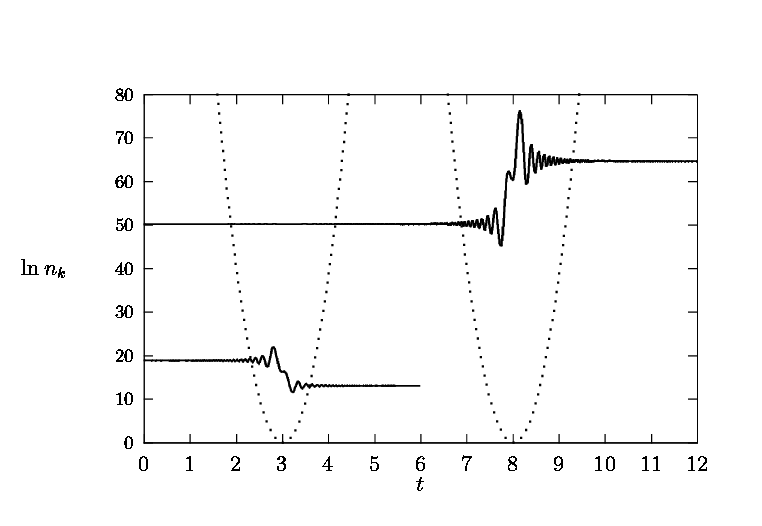
\includegraphics[width=0.65\linewidth, height=0.4\textheight]{Images/Chap4/Linde_Fig8}
	\caption{The change  of the comoving particle number $ n_{k} $ due to scattering at the parabolic potential. The dotted lines show the sequence of the parabilic potentials $ g^{2}\phi^{2}(t) \simeq g^{2}\Phi^{2}m^{2}(t-t_{j})^{2} $ where scattering occurs. Time is given in units of 2$\pi$/$\kappa$. The number of particles can either increase or decrease at the scattering, depending on the phase of the incoming wave \cite{Chap4:LindePreheatingModel}.}
	\label{fig:lindefig8}
\end{figure}
Consider the mode equation around a single parabolic potential. Around the time $ t_{j} $, we can write
\begin{equation}
	\label{Chap4:EquationXkAroundtj}
	\frac{d^{2}X_{k}}{dt^{2}} + \Bigg(\frac{k^{2}}{a^{2}} + g^{2}\Phi^{2}m^{2}(t-t_{j})^{2}\Bigg)X_{k}=0.
\end{equation}
We can rewrite this equation in the simple form 
\begin{equation}
	\label{Chap4:EquationXkAround2}
	\frac{d^{2}X_{k}}{d\tau^{2}} + (\kappa^{2} + \tau^{2})X_{k}=0,
\end{equation}
where we have introduced a new time variable $ \tau \equiv k_{*}(t-t_{j}) $ and a scaled momentum $ \kappa = k/ak_{*} $. Moreover, we have in this case $ \kappa^{2} = (A_{k}-2q)/2\sqrt{q} $. The asymptotes of this equation match the forms (\ref{Chap4:ParabolicPotential_scatter1}) and (\ref{Chap4:scattering2}). We can then interpret $ R_{k} $ and $ D_{k} $ as, respectevely, the reflection and transmission amplitudes of scattering at $ t_{j} $ of scattering at the parabolic potential. The reflection and the transmission coefficients, for consistency, must obey the equation $ |R_{k}^{j}|^{2}  +  |D_{k}^{j}|^{2} = 1$.

The reflection $ R_{k} $ and the transmission  $ D_{k} $ amplitudes can be found using  the linear combination of the parabolic cylinder functions $ W\Big(-\frac{\kappa^{2}}{2};\sqrt{2}\tau\Big) $, and take the form:
\begin{equation}
R_{k}=-\frac{ie^{i\varphi_{k}}}{\sqrt{1+e^{\pi \kappa^{2}}}},
\end{equation}
\begin{equation}
	D_{k} = \frac{e^{-i\varphi_{k}}}{\sqrt{1+e^{-\pi \kappa^{2}}}},
\end{equation}
where the angle $ \varphi_{k} $ is
\begin{equation}
\label{Chap4:angleParabolicPotential}
\varphi_{k}=arg\ \Gamma\Bigg(\frac{1+i\kappa^{2}}{2}\Bigg) + \frac{\kappa^{2}}{2}\Bigg(1+\ln \frac{2}{\kappa^{2}}\Bigg).
\end{equation}
Using these expressions in (\ref{Chap4:ScatteringMatrices}), we obtain the evolution of the amplitudes $ \alpha^{j}_{k},\ \beta_{k}^{j} $ from a single parabolic scattering in terms of the parabolic potential and the phase $ \theta_{k}^{k} $ only, that become
\begin{equation}
	\label{Chap4:scatteringMatrix2}
		\left(
	\begin{array}{c}
		\alpha_{k}^{j+1} \\
		\beta_{k}^{j+1}
	\end{array}
	\right)
	=
	\left(
	\begin{array}{cc}
		\sqrt{1+e^{-\pi \kappa^{2}}}e^{i\varphi_{k}}  & ie^{-\pi \kappa^{2}/2 + 2i\theta^{j}_{k}} \\
		-ie^{-\pi \kappa^{2}/2 - 2i\theta^{j}_{k}} & \sqrt{1+e^{-\pi \kappa^{2}}} e^{-i\varphi_{k}}
	\end{array}
	\right)
	\left(
	\begin{array}{c}
		\alpha_{k}^{j}	\\
		\beta_{k}^{j}
	\end{array}
	\right).
\end{equation}
Now, the number density of $\chi$-particles with momentum \textbf{k} is given by $ n_{k} = |\beta_{k}(t)|^{2} $. Then, from this equation we can calculate the number density of outgoing particles $ n_{k}^{j+1}=|\beta_{k}^{j+1}|^{2} $ after the scattering on the parabolic potential with $ n_{k}^{j}=|\beta_{k}^{j}|^{2} $ incoming particles. We obtain
\begin{equation}
\label{Chap4:parabolicPotentialParticles}
n_{k}^{j+1}=e^{-\pi \kappa^{2}} + \Bigg(1+2e^{-\pi \kappa^{2}}\Bigg)n^{j}_{k} - 2e^{-\pi \kappa^{2}/2}\sqrt{1+e^{-\pi \kappa^{2}}}\sqrt{n_{k}^{j}(1+n_{k}^{j})}\sin \theta^{j}_{tot},
\end{equation}
where $ \theta^{j}_{tot}=2\theta^{j}_{k} - \varphi_{k} + arg \beta_{k}^{j} - arg \alpha_{k}^{j} $. 

Now, we should make two important comments. First, the number of created particles is a step-like function of time. The value $ n_{j}^{k} $ is  constant between two successive scatterings at the points $ t_{j} $ and $ t_{j+1} $. We have a change of the number of particles exactly at the instances $ t_{j} $ in a step-like manner.

The second point is that the effect of particle creation is significant if $ \pi \kappa^{2} \le 1 $, otherwise the exponential term $ e^{-\pi\kappa^{2}} $ suppresses the effect of particle accumulation. We then obtain the following criterion for the width of the resonance band,
\begin{equation}
\label{Chap4:constraintResonanceBand}
\kappa^{2} = \frac{A-2q}{2\sqrt{q}} \le \pi^{-1}.
\end{equation}
Recalling that $ A=\frac{k^{2}}{a^{2}m^{2}} + 2q $ and $ q=\frac{g^{2}\Phi^{2}}{4m^{2}} $, we can rewrite this condition as
\begin{equation}
\label{Chap4:resonanceBand}
\frac{k^{2}}{a^{2}} \le \frac{k_{*}^{2}}{\pi} = \frac{gm\Phi}{\pi}.
\end{equation}
Finally, we can consider the large occupation limit of (\ref{Chap4:parabolicPotentialParticles}), $ n_{k} \gg 1 $,
\begin{equation}
	\label{Chap4:nkLargeOccupation}
	n_{k}^{j+1} \simeq \Bigg(1 + 2 e^{-\pi\kappa^{2}} -2\sin\theta^{j}_{tot}e^{-\pi\kappa^{2}/2}\sqrt{1+e^{-\pi\kappa^{2}}}\Bigg)n_{k}^{j}.
\end{equation}
The first two terms in this equation correspond to the effect of spontaneous particle creation, which always increases the number of particles. The last term corresponds to the induced particle creation, which can either increase or decrease the number of particles. The whole effect of particle creation depends crucially on the interference of the wave functions, i.e. the phase correlation/anticorrelation between successive scatterings at the parabolic potential. The beheaviour of the resonance essentially depends on the beheaviour of the phase $ \theta_{k}^{j} $ as a function of $ k $ for different time intervals $ j $.

In this treatment we now take into account the expansion of the universe. In the case with broad resonance, where $ q\gg 1 $, this parameter significantly varies within a few inflaton oscillations. However, we can treat also this case with the method of successive parabolic scattering and, in this case, (\ref{Chap4:nkLargeOccupation}) simplifies. The reason is that for large initial values of $ q $, the phase variations are much larger than $ \pi  $ for all relevant $ k $ (see \cite{Chap4:LindePreheatingModel}). Therefore, all the phases $ \theta_{j} $ can be considered as random numbers.

Moreover, the backreaction of created particles leads to an exponentially rapid decrease of $ q $ down to $ q \sim 1/4 $ only at the last moments of preheating. Thus, the parameter $ q $ in this regime remains very large and the phases remain random until the very last stages of preheating.

The stochastic character of the phases $ \theta_{k}^{j} $ simplifies significantly (\ref{Chap4:nkLargeOccupation}) since there is no memory in the phase and each scattering can be considered  independent from the previous ones.
Assuming then $\theta_{tot}$ completely random, we can rewrite (\ref{Chap4:nkLargeOccupation}) as
\begin{equation}
\label{Chap4:numberkRandom}
	n_{k}^{j+1} \simeq \Bigg(1 + 2 e^{-\pi\kappa_{j}^{2}} -2\sin\hat{\theta}e^{-\pi\kappa_{j}^{2}/2}\sqrt{1+e^{-\pi\kappa_{j}^{2}}}\Bigg)n_{k}^{j},
\end{equation}
where $\hat{\theta}$ is a random phase in the interval $ (0,2\pi) $, and $ k_{j}^{2} $ changes slowly with $ j $, $\kappa_{j}^{2} \sim j^{-1/3}$.
This equation defines the number of particles at an arbitrary moment as a function of the random phase. Then, the number of particles $ n_{k}^{j} $ is a random variable which can either increase or decrease depending on the realitation of the phase. The whole process is the superposition of elementary processes where $ n_{k} $ jumps up and down. However, on average the number of particles is amplified with time. This means that $ n_{k} $ increases more often than it decreases. Indeed, from the analysis of \cite{Chap4:LindePreheatingModel} comes out that the probability for the number of particles to increase is three times higher than the probability of its decreasing. There is also a natural selection effect. Among all modes $ \chi_{k} $, there will be some modes for which the increasing appears more often than in the proportion $ 3:1 $. These modes will give the dominant contribution to the total number of produced particles.

When the parameter $ q $ decreases because of the expansion of the universe and becomes smaller than 1, the resonance becomes similar to the usual parametric resonance with $ q\le 1 $. However, at some stage this description needs to be corrected because of the backreaction of the created particles.

\section{Backreaction and Rescattering}
In the preheating epoch we have a resonant amplification of the fluctuations $ \chi_{k}(t) $, which corresponds to an exponentially fast creation of $ n_{k} $ particles. However, because of the exponential  instability of the $\chi$-field, we expect that its backreaction on the background gradually accumulate until it affects the process of resonance itself. Therefore, we can divide preheating in two stages. In  the first part of preheating  the backreaction of created particles can be neglected. This stage is rather long, and if the initial value of $ q $ is small enough, i.e $ q_{0} \le 10^{3} $, preheating may end before backreaction becomes important. Instead, in the case in which $ q_{0} $ is greater than $ 10^{3}$, at some moment we have to change the description of the parametric resonance.

We can have several ways in which backreaction can alter the process. First, interactions with particles created by parametric resonance may change the effective masses of all particles and the frequency of oscillation of the inflaton field. Moreover, scattering of the particles off each other and their interaction with the oscillating field $ \phi(t) $ may lead to additional particle production and to the removal of the previously produced particles from the resonance.

Then, we have to take into account two effects. First, $\chi$-particles may change the frequency of oscillations of the inflaton field $ \phi(t) $. This can lead to an increase of the value of $ m $, making the resonance narrow and eventually shut it down.

The second effect is that the interaction of $ \chi $-particles with the oscillating field $ \phi(t) $ may lead to the production of $ \phi $-particles. Indeed, we can imagine this process as scattering of $ \chi $-particles on the oscillating inflaton field $ \phi(t) $. In each interaction each $\chi$-particle takes one $\phi$-particle away from the homogeneous oscillating field $ \phi(t) $. When many $\phi$-particles are produced, they may change the effective mass of the field $\chi$, making $ \chi $-particles so heavy that they no longer can be produced. Moreover, the process of rescattering can destroy the inflaton field $ \phi(t) $ by decomposing it into separate $ \phi $-particles. For references of this section see \cite{Chap4:LindePreheatingModel},\cite{Chap4:Reference1} and \cite{Chap4:Reference2}. Here we summarise the main points.

The simplest way to take into account the backreaction of the amplified quantum fluctuations $ \chi_{k} $ is to use the Hartree, or mean-field, approximation. In this approximation we assume that different modes and fields evolve independently (are uncorrelated in time), i.e.
 $ \langle \chi^{*}_\textbf{k-q}\chi_{\textbf{k}}\rangle \ \simeq 0 $ if $\textbf{q}\neq 0$, $\langle \delta \phi^{*}_\textbf{k-q}\chi_{\textbf{k}}\rangle \ \simeq 0 $ etc. for all $ q $.  In this way all effects of the amplification of the $\chi$-field are mediated by the variance of $\chi$, $ \langle \chi^{2}\rangle  $. 
 
In the Hartree approximation the equation for the field $\phi$ reads
\begin{equation}
\label{Chap4:Backreaction_HartreeApproximation}
\ddot{\phi} + 3H\dot{\phi} + m^{2}\phi + g^{2}\chi^{2}\rangle  \phi=0,
\end{equation}
where the vacuum expectation value $ \langle \chi^{2}\rangle   $ is
 \begin{equation}
\label{Chap4:Backreaction_vevChi2}
\langle \chi^{2}\rangle  =\frac{1}{2\pi^{2}a^{3}}\int_{0}^{\infty} dk\  k^{2}|\chi_{k}(t)|^{2}.
\end{equation}
Quantum effects contribute to the effective mass $ m_{\phi} $ of the inflaton field. Indeed, from (\ref{Chap4:Backreaction_HartreeApproximation}) we have that $ m_{\phi}^{2}=m^{2} + g^{2}\langle \chi^{2}\rangle   $. 

One can express $ \langle \chi^{2}\rangle   $ in terms of the coefficients $ \alpha_{k}(t) $ and $\beta_{k}(t)$ that describe the resonance \cite{Chap4:LindePreheatingModel}:
\begin{equation}
\label{Chap4:Backreaction_ExpressionFluctuation}
\langle \chi^{2}\rangle   = \frac{1}{2\pi^{2}a^{3}}\int_{0}^{\infty} \frac{dk k^{2}}{\omega} \Bigg(|\beta_{k}|^{2} + Re\Bigg(\alpha_{k}\beta_{k}^{*}e^{-2i\int_{0}^{t} \omega dt}\Bigg)\Bigg).
\end{equation}
Using the fact that $ n_{k}=|\beta_{k}|^{2} $, we can express the effective mass squared  of the background field $\phi(t)$ in the Hartree approximation as \cite{Chap4:LindePreheatingModel}
\begin{equation}
\label{Chap4:Backreaction_EffectiveMass}
m^{2}_{\phi}=m^{2} + \Bigg(1 + C\cos\Bigg( \frac{2g\Phi}{m} \cos mt \Bigg) \Bigg) \frac{gn_{\chi}}{|\phi(t)|},
\end{equation}
where $ C $ is a numerical factor that derives from the integration. 

The equation for the inflaton field becomes
\begin{equation}
\label{Chap4:Backreaction_equationInflaton}
\ddot{\phi} + 3H\dot{\phi} + m^{2}\phi + gn_{\chi}\Bigg(1 + C\cos \frac{2g\Phi 	\cos mt}{m}\Bigg) \frac{\phi}{|\phi|} = 0.
\end{equation}
The last term oscillates with a frequency $\sim 2g\Phi \gg m$. However, in the broad resonance regime with $ g\Phi \gg m $, the high frequency oscillation does not much affect the evolution of the field $ \phi(t) $, and then we can neglect it.
Thus, in the first approximation the equation for the inflaton field reads
\begin{equation}
	\label{Chap4:Backreaction_EquationPhiFinal}
	\ddot{\phi} + 3H\dot{\phi} + m^{2}\phi + gn_{\chi}\frac{\phi}{|\phi|} = 0.
\end{equation}
To estimate the change of the frequency of the oscillations of the inflaton field we can use the effective mass $ m^{2}_{\phi}=m^{2} + g^{2}\langle \chi^{2}\rangle  $. We obtain that the frequency of oscillations of the inflaton field does not change until the number of $ \chi $-particles grows to 
\begin{equation}
\label{Chap4:Backreaction_CriterionFirstStage}
n_{\chi} \simeq \frac{m^{2}\Phi}{g}=\frac{2m^{3}}{g^{2}}q^{1/2}.
\end{equation}
We can use this value to define the duration of the first stage of preheating where  backreaction of the created particles can be neglected. 

Therefore, we obtain the following picture (see \cite{Chap4:LindePreheatingModel}). The process of broad resonance can be divided in two stages. In the first stage, $ n_{\chi} \ll m^{2}\Phi/g $, backreaction of the $ \chi $-particles can be neglected and the frequency of oscillations of the field $ \phi $ is determined by its bare mass $ m $. The second stage begins when $ n_{\chi} \sim m^{2}\Phi/g $. From now, the frequency of oscillations of the field $\phi$ becomes determined not by its bare mass $ m $, but by its interaction with $\chi$-particles.

There is another process that affect the preheating stage. We should consider also the generation of inflaton fluctuations $\delta \phi$ due to the interaction of $\chi$-particles with the oscillating field $\phi(t)$ and the subsequent interaction between $\chi$ and $\delta \chi$ fluctuations. Using a \textit{particle-like} picture we can imagine the classical scalar field as a condensate of $\phi$-particles with zero momentum, and interpret $\phi$-particle production as the result of rescattering of $ \chi $-particles in the condensate. With this interpretation, we can use the concept of cross-section of interacting particles. Actually, the process is very complicated and this interpretation fails (see the discussion in \cite{Chap4:LindePreheatingModel}). However, there are two results that are valid. First, there is a significant generation of rapidly growing fluctuations $ \delta \phi \sim e^{2\mu m_{\phi}t} $, due to the interaction between $ \chi $-particles and the oscillating inflaton field $ \phi(t) $. Second, the generation of large fluctuations of $\delta \phi$ can terminate the resonant creation of $\chi$-particles at the end of the second stage of preheating. 

 We discuss now briefly the validity of the Hartree approximation. In fact, as the number of particles increases the Hartree approximation stops to  being a good description. The couplings between different Fourier modes become important, heralding the true beginning of the non-linear stage.  
However, we will discuss this important result. Fluctuations of the $\chi$-fields generated from vacuum by the oscillating inflaton in the large occupation number limit can be considered as classical waves with gaussian statistics. Therefore, in first approximation all fields $\chi$, $\delta \phi$ can be treated as interacting scalar waves. We can then study preheating by investigating  a system of non-linear classical equations or by lattice numerical simulations of the interacting scalar fields. The equations of motion in Fourier space for the Fourier modes of the fluctuations $\delta \phi$ are:
\begin{equation}
\label{Chap4:Backreaction_EquationDeltaPhi}
\ddot{\delta \phi_{k}} + 3H\delta \dot{\phi}_{k} + \Bigg(\frac{k^{2}}{a^{2}} + m^{2}_{\phi}\Bigg)\delta \phi_{k}
=-\frac{g^{2}\phi_{0}(t)}{(2\pi)^{3}} \int d^{3}k' \chi_{\textbf{k} - \textbf{k'}}\chi_{\textbf{k}'} - \frac{g^{2}}{(2\pi)^{3}}\int d^{3}k'\ d^{3} k'' \delta\phi_{\textbf{k}-\textbf{k}' + \textbf{k}''}\ \chi_{\textbf{k}'}\chi_{\textbf{k}''},
\end{equation}
and those for $ \chi_{k} $:
\begin{equation}
\label{Chap4:Backreaction_EquationChi}
\ddot{\chi_{k}} + 3H\dot{\chi}_{k} + \Bigg(\frac{k^{2}}{a^{2}} + g^{2}\phi_{0}^{2}(t)\Bigg)\chi_{k}
=-\frac{g^{2}\phi_{0}(t)}{(2\pi)^{3}} \int d^{3}k' \chi_{\textbf{k} - \textbf{k'}}\delta\phi_{\textbf{k}'} - \frac{g^{2}}{(2\pi)^{3}}\int d^{3}k'\ d^{3} k''\chi_{\textbf{k}-\textbf{k}' + \textbf{k}''}\ \delta\phi_{\textbf{k}'}\delta\phi_{\textbf{k}''}.
\end{equation}
 The Hartree approximation corresponds to neglect the scattering between different Fourier modes. Considering the first equation, only the second term in the r.h.s is retained. This term gives rise only to the  $ g^{2}\langle \chi^{2}\rangle  \delta\phi_{k} $ term for \textbf{k}'=\textbf{k}'' . The other term in this equation is neglected because involves coupling between different Fourier modes. Similarly, we obtain $ g^{2}\langle \delta \phi^{2}\rangle \chi_{k} $ from the r.h.s of the second equation. Therefore, the perturbed field equations under the Hartree approximation
 are
 \begin{equation}
\label{Chap4:Backreaction_deltaPhiHartree}
\ddot{\delta \phi_{k}} + 3H\delta \dot{\phi_{k}} + \Bigg(\frac{k^{2}}{a^{2}} + m^{2}_{\phi} + g^{2}\langle \chi^{2}\rangle  \Bigg)\delta\phi_{k} = 0,
 \end{equation}
\begin{equation}
\label{Chap4:Backreaction_deltaChiHartree}
\ddot{\chi_{k}} + 3H \dot{\chi}_{k} + \Bigg(\frac{k^{2}}{a^{2}} + g^{2}(\phi_{0}^{2}(t) + \langle \delta \phi^{2}\rangle  )\Bigg)\chi_{k}=0.
\end{equation}
The scattering between different momentum modes becomes crucial especially  at the non linear stage of preheating, and then we cannot have a complete view with the Hartree approximation. Indeed, the couplings between different Fourier modes actually lead  the rescattering process.

The equations (\ref{Chap4:Backreaction_EquationDeltaPhi}) and (\ref{Chap4:Backreaction_EquationChi}) explain also an observation of the lattice simulations. After the initial resonance in the $\chi$-field, there is a very rapid amplification of the fluctuations of the inflaton field. We can see this by looking at the first term on the r.h.s. of (\ref{Chap4:Backreaction_EquationDeltaPhi}). This term is independent of $\delta \phi_{k}$, which grows as $ \exp(2\mu_{k}m_{\phi}t) $ since each factor of $\chi$ is growing  exponentially with Floquet index $\mu$. This provides a rapid increasing source term for $\delta \phi_{k} $ fluctuations. Then, the fluctuations $\delta \phi_{k}$ goes as $ \delta \phi_{k} \sim e^{2\mu m_{\phi}t} $ and hence they  will grow basically with twice the Floquet index of the $\chi$-fluctuations (see Fig. (\ref{fig:nonlineardynamics}) from \cite{Chap4:Reference2} and \cite{InflationDynamicsAndReheating:chap1}).  

\begin{figure}
	\centering
	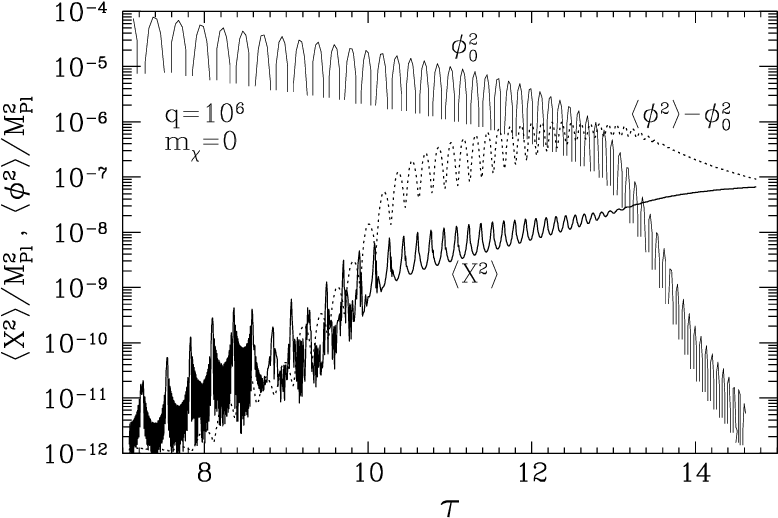
\includegraphics[width=0.6\linewidth, height=0.35\textheight]{Images/Chap4/NonLinearDynamics}
	\caption{Lattice simulations for the evolution of the field  variances in the $\phi$ and $\chi$ fields during preheating for the model $ V(\phi,\chi)=\frac{1}{2}m^{2}\phi^{2} + \frac{1}{2}g^{2}\phi^{2}\chi^{2} $ with an initial resonance parameter $ q=10^{6} $. Here $\tau$  is the conformal time and $ \langle X^{2}\rangle  $ is $ \langle \chi^{2}\rangle   $ in our notation. The $\chi$ fluctuations begins to grow initially through parametric resonance but this is followed by the growth of the $\phi$ fluctuations through the non-linear process of rescattering which is significantly more rapid (with roughly double the Floquet index). The backreaction shuts off the resonance in the $\chi$-field earlier than it does in the $\phi$ fluctuations which also dominate the final variances. The lattice simulations are essential to full understand the process \cite{Chap4:Reference2}, \cite{InflationDynamicsAndReheating:chap1}. }
	\label{fig:nonlineardynamics}
\end{figure}
 We can then put all together to summarise all the stages of preheating making some important comments.
In the first stage we can ignore the backreaction of created particles on the frequency of oscillations of $ \phi(t) $. An estimate of the moment $ t_{1} $ in which this stage ends is 
\begin{equation}
\label{Chap4:estimate}
n_{\chi}(t_{1}) \simeq \frac{m^{2}\Phi(t_{1})}{g}.
\end{equation}
A very important point is which fluctuations $\chi_{k}$ are amplified during the entire period of resonance. We remind that the amplification occurs when the adiabaticity condition $ \frac{d\omega}{dt} \langle  \omega^{2} $ is violated, i.e. when the inflaton field $ \phi(t)=0 $. This implies that the  fluctuations $\chi_{k}$ amplified by the broad resonance have physical momenta $ k \le k_{*}/2 \sim  \sqrt{gm\Phi}/2 $. In other words, we  obtain an exponentially growing occupation number of particles with $ k < k_{m} $, i.e. $ n(t) \sim \exp(2\mu m t) $, where $\mu$ is an effective index which describes an average rate of growth for modes with $ k<k_{*} $. Meanwhile, the amplitude $\Phi$ decreases as $\sim M_{pl}/3mt$ due to the expansion of the universe.

 For different values of the coupling constant $ g $, one can estimate for example the initial value $ q_{0} $ and the final value $ q_{1} $ of $ q $ at the  beginning/end of the first stage of preheating. We report the results of \cite{Chap4:LindePreheatingModel}. For $ g \simeq 10^{-3}$, we have $q_{0}\simeq 10^{4} $ and $ q_{1}\simeq 3 $. For $ g \simeq 10^{-2} $, we have $q_{0} \simeq 10^{6} $ and $ q_{1}\simeq 550 $. Finally, for $g\simeq 10^{-1} $, $ q_{0}\simeq 10^{8} $ and $ q_{1} \simeq 10^{5} $. One can also calculate the number of oscillations the inflaton field $ \phi $ makes from the end of inflation to the end of the first stage. For example, the inflaton makes 15, 11 and 8 oscillations for the three different couplings reported above, respectevely.
 
 From the analysis of \cite{Chap4:LindePreheatingModel} we can distinguish different scenarios depending on the coupling constant $ g $. For $ g \ll 3 \times 10^{-4} $, the broad resonance ends during the first stage. Parametric resonance in this case is not efficient enough to transfer the main part of energy of the inflaton field to the energy of  $\chi$-particles. 
 
 For $ g\sim 3 \times 10^{-4} $, at the end of the first stage we have $ q_{1} \sim 1/4 $. The energy becomes approximately equally distributed between the energy of the oscillating inflaton field $\phi$ and the energy of the $\chi$-particles produced by its oscillations.
 
 Finally, for $ g > 3 \times 10^{-4} $ the broad resonance continues after  the end of the first stage.  To study further the process, one should study quantum effects produced by the interaction of the $ \chi $-fluctuations with the oscillating inflaton field $\phi(t)$.
 
 In the second stage of preheating (after $ t_{1} $) the frequency  of inflaton oscillations is determined by the backreaction of $ \chi $-particles and it is no longer $ m $.
 Neglecting rescattering for the moment, from the numerical analysis of \cite{Chap4:LindePreheatingModel}, comes out that the system  spends half of the time in the broad resonance regime and another half of the time in the regime with $ q \sim 1 $. During all the time, except the last one or two oscillations, the parameter $ q $ is very large and the theory can be described with the stochastic resonance. When $ q\sim 1/4 $, the resonance terminates. However, this description should be modified because of the presence of the rescattering process. 
 
 The rescattering process leads to the fragmentation of the inflaton condensate. In  order to alter the motion of the field the fluctuations $ \delta \phi $ should have comparable kinetic energy to $ m_{\phi}\Phi^{2}/2 $. The fluctuations of the inflaton field $\delta \phi $ grow as $\delta \phi \sim e^{2\mu m t}$, due to the interactions of pairs of $\chi$-particles with the inflaton condensate. In this stage the inflaton fluctuations grows with double rate. When $ \langle \delta \phi^{2}\rangle \ \gg \Phi^{2}  $ we say that the condensate is substantially fragmented or destroyed. Then, rescattering also re-destributes the energy stored in the $\chi$-particles. The rescattering process transfers the energy from the amplified  modes to modes with momenta lying in the stability regions. Even if rescattering completely shuts off the resonance, rescattering becomes important since leads to the non-linear evolution of the system and to the fragmentation of the inflaton condensate.
 
 However, we should point out that having a fragmented inflaton condensate does not imply that the energy stored in it is negligible. We can say only that rescattering and fragmentation kick in when the energy stored in interaction terms and/or fluctuations is comparable to the energy of the classical background. Then, at the end of preheating, non-perturbative particle production ends and non-linear evolution begins with most (or at least non-negligible) fraction of the total energy being stored in field fluctuations.
 
  We can roughly estimate the time at which resonance ends comparing the effective mass term of the inflaton field $ g^{2}\langle \chi^{2}\rangle  $ with its squared bare mass $ m^{2} $. When  backreaction of the $\chi$ fluctuations are as large as the inflaton bare mass it is difficult for the resonance to continue. Considering that $ \langle \chi^{2}\rangle  \sim e^{2\mu m t} $, we obtain
 \begin{equation}
t_{end} \sim \frac{1}{\mu m}\ln\Bigg(\frac{m}{g}\Bigg).
 \end{equation}
 From the analysis of \cite{Chap4:LindePreheatingModel} comes out that, for example, at the end of resonance $\chi$-particles need to rescatter only 10 times to destroy the coherent oscillation of the field $\phi$ and decomposing it into separate $\phi$-particles. At the end of resonance, $\chi$-particles may destroy the classical field $\phi(t)$ completely. Then, the final stage of preheating is not determined by resonance, but by rescattering.  
 
 In the next chapter we will investigate through numerical simulations in the literature this peculiar stage. Before doing that, we explore now other models of preheating.

 \section{Model $\lambda \phi^{4}$}
 In this section we concentrate on the theory of preheating in a class of conformally invariant theories such as $ \frac{\lambda}{4} \phi^{4} + \frac{1}{2}g^{2}\phi^{2}\chi^{2} $. In such theories, the classical oscillating inflaton field $\phi(t)$ decays into $\chi$-particles and $\phi$-particles. The parametric resonance in this theory is described by the Lame equation and significantly differs from the resonance with a quadratic potential. The structure of the resonance in this case depends in a rather nontrivial way on the parameter $ g^{2}/\lambda $. For example,  with $ g^{2}=\lambda $ or $ g^{2}=3\lambda $ this theory has only one instability band, but the structure of the bands and the characteristic exponents $\mu_{k}$ are completely dfferent. Changing the ratio $ g^{2}/\lambda $ only slightly, the number of instability bands immediately becomes infinitely large.
 In this section we review the model. For reference and details see \cite{Chap4:ModelLambdaPhi4Reference}.
 
\subsection{Equation for the inflaton}
In the chaotic inflation model $ V(\phi)=\frac{1}{4} \lambda \phi^{4}$ the equation for the classical field $\phi(t)$ reads
\begin{equation}
\label{Chap4:lambdaPhi4_eomPhi4}
\ddot{\phi} + 3H\dot{\phi} + \lambda \phi^{3}=0.
\end{equation}
 For sufficiently large initial values $\phi > M_{pl}$, the friction term $ 3H\dot{\phi} $ dominates over $\ddot{\phi}$. This leads to the inflationary stage where the universe expands quasi-exponentially. With a decrease of the field $\phi$ below $ M_{pl} $, the friction term $ 3H\dot{\phi} $ becomes less important and inflation terminates at $ \phi \sim M_{pl}/2 $. After a short stage of fast rolling down, the inflaton rapidly oscillates around  the minimum of $ V(\phi) $ with  initial amplitude $ \Phi_{0} \sim 0.1 M_{pl} $.
 
 The amplitude $\Phi$ of the oscillations of the inflaton field $\phi$ after inflation asymptotically approaches
 \begin{equation}
\label{Chap4:lambdaPhi4_inflaton}
\Phi(t) \simeq \frac{1}{\sqrt{t}}\Bigg(\frac{3M_{pl}^{2}}{8\pi \lambda}\Bigg)^{1/4} \sim \frac{M_{pl}}{10N},
 \end{equation}
 where $ N $ is the number of oscillations after the end of inflation.
 
 To simplify calculations in this theory we make a conformal transformation of the space-time metric and the fields. We then use the conformal time
 \begin{equation}
\label{Chap4:ConformalTime}
\eta = \int \frac{dt}{a(t)},
 \end{equation}
 and the conformal field,
 \begin{equation}
 	\label{Chap4:lambdaPhi4_ConformalField}
\varphi = a\phi.
 \end{equation}
 In the coordinates $ (\eta,\textbf{x}) $ the equation of motion for the field $\phi$ (\ref{Chap4:lambdaPhi4_eomPhi4}) becomes 
 \begin{equation}
\label{Chap4:labdaPhi4_eomPhi2}
\varphi'' + \lambda\varphi^{3} - \frac{a''}{a}\varphi=0.
 \end{equation}
 However, the last term in this equation can be discarded. Indeed, in this particular model after inflation we have a radiation-like dominated era, $ p=\rho/3 $,  $ a(\eta) \sim \eta $ and then $ a''= 0 $. The equation (\ref{Chap4:labdaPhi4_eomPhi2}) now reads simply
 \begin{equation}
 	\label{Chap4:labdaPhi4_eomPhi3}
 	\varphi'' + \lambda\varphi^{3}=0.
 \end{equation}
 This equation can be reduced to the canonical equation for an elliptic function. We use the dimensionless conformal time variable
 \begin{equation}
\label{Chap4:lambdaPhi4_conformalTimeVariable}
x\equiv \sqrt{\lambda} \tilde{\varphi}\eta = \Bigg( \frac{6\lambda M_{pl}^{2}}{\pi}\Bigg)^{1/4}\sqrt{t},
 \end{equation}
 where $\tilde{\varphi}$ is the amplitude of the oscillations of the field $\varphi$. We rescale the field $\varphi$ as $\varphi=\tilde{\varphi}f(x)$, where the function $ f(x) $ has an amplitude equal to unity. This function  obeys to the canonical equation for elliptic functions
 \begin{equation}
 	\label{chap4:lambdaPhi4_EllipticFunction}
 	f'^{2}(x)=\frac{1}{2}(1-f^{4}),
 \end{equation}
 whose solution is in terms of the elliptic cosine
 \begin{equation}
\label{Chap4:lambdaPhi4_solutionF(x)}
	f(x)=cn\Bigg(x-x_{0};\frac{1}{\sqrt{2}}\Bigg).
 \end{equation}
 Oscillations in this theory are not sinusoidal, but are given by an elliptic function. Moreover, the energy density of the inflaton field $\phi$ decreases in the same way as the density of radiation, i.e. $ a^{-4} $.
 
 The elliptic cosine can be represented as follows \cite{Chap4:ModelLambdaPhi4Reference}:
 \begin{equation}
\label{Chap4:lambdaPhi4_EllipticCosineForm}
f(x)=\frac{8\pi\sqrt{2}}{T}\sum_{n=1}^{\infty}\frac{e^{-\pi(n-1/2)}}{1+e^{-\pi (n-1/2)}}\cos \frac{2\pi (2n-1)x}{T},
 \end{equation}
 where $ T \simeq 7.416 $ is the period of oscillations. In this equation the amplitude of the first term in the sum is 0.9550; the amplitude of the second term is much smaller, 0.04305. However, even if the first harmonic term is very close to the actual form of oscillations, to study the general structure of stability/instability bands one should consider the full solution.
 
 \subsection{Conformal theory}
 Consider the interaction between the classical inflaton field $\phi$ and the massless quantum scalar field $\chi$, given by the lagrangian
 \begin{equation}
\label{Chap4:lambdaPhi4_Lagrangian}
\mathcal{L}=\frac{1}{2}\partial_{\mu}\phi\partial^{\mu}\phi - \frac{\lambda }{4}\phi^{4} + \frac{1}{2}\partial_{\mu}\chi\partial^{\mu}\chi - \frac{1}{2}g^{2}\phi^{2}\chi^{2}.
 \end{equation}
 The fluctuations of the $\chi_{k}$-field with comoving momentum \textbf{k} obeys the equation
 \begin{equation}
\label{Chap4:lambdaPhi4_EquationChi}
\ddot{\chi}_{k} + 3\frac{\dot{a}}{a}\dot{\chi}_{k} + \Bigg(\frac{k^{2}}{a^{2}} + g^{2}\phi^{2}\Bigg)\chi_{k}= 0.
 \end{equation}
 The self-interaction $\lambda\phi^{4}$ also leads to the generation of fluctuations of the field $\phi$. The equation for the inflaton field $\phi_{k}$
is 
\begin{equation}
\label{Chap4:lambdaPhi4_EquationPhik}
\ddot{\phi}_{k} + 3\frac{\dot{a}}{a}\dot{\phi}_{k} + \Bigg(\frac{k^{2}}{a^{2}} + 3\lambda\phi^{2}\Bigg) \phi_{k}= 0.
\end{equation} 
Note that this last equation is equal to (\ref{Chap4:lambdaPhi4_EquationChi}) with $ g^{2}=3\lambda $. Then, the last equation is a particular case of (\ref{Chap4:lambdaPhi4_EquationChi}). Since the physical momentum $ \textbf{p}=\textbf{k}/\textbf{a(t)} $ in (\ref{Chap4:lambdaPhi4_EquationChi}) is redshifted in the same manner as the background field $ \phi(t) = \varphi(t)/a(t) $, we can eliminate the redshifting of momenta from the evolution of $\chi_{k}$. In fact, considering the rescaled quantity $ X_{k}(t) = a(t)\chi_{k}(t) $ and rewriting the mode equation for $ X_{k}(t) $ with the conformal time $ x $, we obtain
\begin{equation}
\label{Chap4:lambdaPhi4_modeEquation}
X_{k}'' + \Bigg(\kappa^{2} + \frac{g^{2}}{\lambda}cn^{2}\Bigg(x,\frac{1}{\sqrt{2}}\Bigg)\Bigg)X_{k} = 0,
\end{equation}
where $\kappa^{2}=k^{2}/\lambda \tilde{\varphi}^{2}$. In this way, the equation for the field fluctuations does not depend on the expansion of the universe and it is reduced to a problem in Minkowsky space-time. This is a special feature of this theory. The equation (\ref{Chap4:lambdaPhi4_modeEquation}) describes oscillators, $ X_{k} $, with a variable frequency
\begin{equation}
\label{Chap4:lambdaPhi4_frequency}
\omega^{2}_{k}=\kappa^{2} + \frac{g^{2}}{\lambda}cn^{2}\Bigg(x;\frac{1}{\sqrt{2}}\Bigg),
\end{equation}
which periodically depends on time, $ x $. For the fluctuations of the field $ \varphi = a\phi $, we have
\begin{equation}
\label{Chap4:lambdaPhi4}
\varphi_{k}'' + \Bigg(\kappa^{2} + 3cn^{2}\Bigg(x,\frac{1}{\sqrt{2}}\Bigg)\Bigg)\phi_{k} = 0.
\end{equation}
The solutions $ X_{k} $ are exponentially unstable, i.e. $ X_{k}(x) \propto e^{\mu_{k}x} $. Assuming positive-frequency initial condition, we expect then an exponentially fast creation of $\chi$-particles as the inflaton field oscillates, i.e. $ n_{k} \sim e^{2\mu_{k}x} $. The parameter $ g^{2}/\lambda $ gives the strength of the interaction with the periodic oscillations $ cn^{2}(x,1/\sqrt{2}) $. Therefore, we have a crucial difference with the theory with a quadratic potential described in the previous section. In the theory with quadratic potential it is required a large amplitude of the inflaton field. In the conformal theory, instead, is the combination of parameters $ g^{2}/\lambda $ that defines the structure of the parametric resonance.

The equation (\ref{Chap4:lambdaPhi4_modeEquation}) belongs to the class of the Lame equations and it is an equation with periodic coefficients, as the Mathieu equation. The solutions $ X_{k} $ of this equation may be stable or unstable depending on the particular values for $ \kappa $ and $ g^{2}/\lambda $. The parameter $ g^{2}/\lambda  $ represents the strength of the interaction. The second parameter $\kappa$ is the momentum of vacuum fluctuations $\kappa$ in units of the frequency of the inflaton oscillations.

As in the quadratic potential model, the evolution of the comoving number density of created $\chi_{k}$-particles, $ n_{k} $ with comoving momentum $ k $, is given by the comoving energy density and the energy per particle $\omega_{k}$,
\begin{equation}
\label{Chap4:lambdaPhi4Model}
n_{k}=\frac{\omega_{k}}{2}\Bigg(|\chi_{k}|^{2} + \frac{|\dot{\chi}_{k}|^{2}}{\omega_{k}^{2}}\Bigg) - \frac{1}{2}.
\end{equation}
\begin{figure}
	\centering
	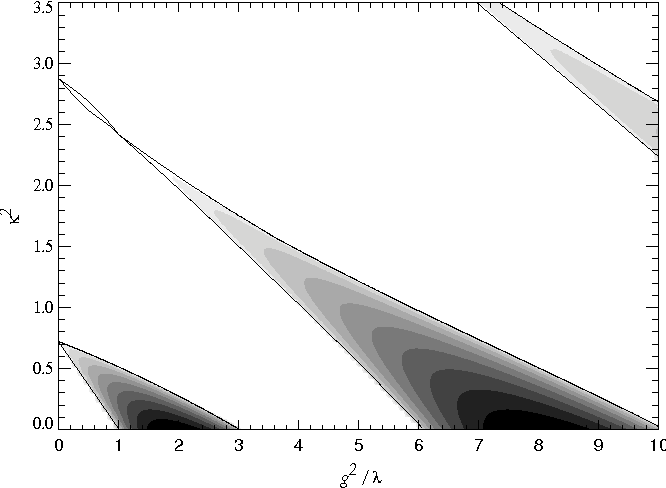
\includegraphics[width=0.6\linewidth, height=0.3\textheight]{Images/Chap4/ConformalTheory_Fig4}
	\caption{The stability/instability chart for the Lame equation for fluctuations $ X_{k}(x) $ in the variables $ (\kappa^{2},\frac{g^{2}}{\lambda}) $, obtained from the numerical solution of (\ref{Chap4:lambdaPhi4_modeEquation}). Shaded (unshaded) areas are regions of instability (stability). For instability bands, the darker shade implies a larger characteristic exponent $\mu_{k}$. There are 10 color steps. One color step corresponds to the increment $\Delta \mu_{k} = 0.0237$, so the darkest shade corresponds to maximal $\mu_{k}=0.237$, the least dark shade in the instability bands correspond to $\mu_{k}=0.009$. For positive $\kappa^{2}$, there is only one instability band for the particular values of the parameter $ \frac{g^{2}}{\lambda}=1 $ and 3. This occurs because the higher bands shrink into nodes as $ \frac{g^{2}}{\lambda} $ approaches 1 and 3 \cite{Chap4:ModelLambdaPhi4Reference}.  }
	\label{fig:conformaltheoryfig4}
\end{figure}

The stability/instability charts of the Lame equation describes preheating in the conformal invariant theories and it is studied in \cite{Chap4:ModelLambdaPhi4Reference}.
The stability/instability chart is plotted in (Fig. \ref{fig:conformaltheoryfig4}) from \cite{Chap4:ModelLambdaPhi4Reference}. The stability/instability chart is similar to the stability/instability chart of Mathieu equation, but there are important differences. In the case of Mathieu equation there are infinitely instability bands corresponding to each value of $ q $. Instead, in the Lame equation some of the instability bands may occasionally shrink to a point. For example, for $ g^{2}/\lambda=1 $ and for $ g^{2}/\lambda=3 $ there is only one instability band. From the (Fig. \ref{fig:conformaltheoryfig4}), indeed, we see that the higher zones shrink to nodes as $ g^{2}/\lambda  $ approaches to 1 and 3. For positive $\kappa^{2}$, whenever $ \frac{g^{2}}{\lambda}=\frac{n(n+1)}{2} $, there are a finite number of instability bands. Finally, as for the Mathieu equation, all other values of $ g^{2}/\lambda $ have infinite numbers of instability bands. 

In particular, for $\frac{g^{2}}{\lambda} \ll 1  $, the Lame equation can be formally transformed into the Mathieu equation with the parameters $ A\simeq 1.3932 \kappa^{2} $ and $ q\simeq 0.3464 \frac{g^{2}}{\lambda} \ll 1 $. Thus, in this case the stability/instability charts of Mathieu equation and Lame equation coincide exactly.
\subsection{Analysis of Lame equation}
The Lame equation can be solved in terms of the transcendental Jacobi functions. The analytical study of resonance using these functions is rather difficult. However, for $\frac{g^{2}}{\lambda}=\frac{n(n+1)}{2}  $, with $ n  $ integer, one can obtain simple solutions to (\ref{Chap4:lambdaPhi4_modeEquation}). In \cite{Chap4:ModelLambdaPhi4Reference} are studied different cases for the value of $ g/\lambda $. Here we summarise the main results.

First, we rewrite (\ref{Chap4:lambdaPhi4_modeEquation}) in the so-called algebraic form using the time variable $ z $ instead of $ x $, where
\begin{equation}
	\label{Chap4:lambdaPhi4}
	z(x)=cn^{2}\Bigg(x,\frac{1}{\sqrt{2}}\Bigg).
\end{equation}
The equation (\ref{Chap4:lambdaPhi4_modeEquation}) becomes
\begin{equation}
\label{Chap4:lambdaPhi4_fluctuations}
2z(1-z^{2})\frac{d^{2}X_{k}}{dz^{2}} + (1-3z^{2})\frac{dX_{k}}{dz} + (\kappa^{2} + \frac{g^{2}}{\lambda}z)X_{k}=0.
\end{equation}
Consider two linearly-independent solutions of this equation, $ X_{1}(z) $ and $ X_{2}(z) $. We expect that one of them exponentially grows and the other exponentially decreases during resonance. Introducing the linear combinations $ X_{1}^{2}, X_{2}^{2} $ and $ X_{1}X_{2} $,  turns out that they solve the third order equation 
\begin{equation}
\label{Chap4:lambdaPhi4_equationForMz}
2z(z^{2}-1)\frac{d^{3}M}{dz^{3}} + (9z^{2}-3)\frac{d^{2}M}{dz^{2}} -2\Bigg[\bigg(2\frac{g^{2}}{\lambda} - 3\bigg)z + 2\kappa^{2}\Bigg]\frac{dM}{dz} - 2\frac{g^{2}}{\lambda}M = 0.
\end{equation}
The three solutions, $ M(z) $, of this equation correspond to the three bilinear combinations of $ X_{1} $ and $ X_{2} $. The important point is that for $ \frac{g^{2}}{\lambda} = \frac{n(n+1)}{2} $ this equation admits a polynomial solution of degree $ n $. This solution is the product of an exponentially growing solution and an exponentially decreasing solution in the resonance zone, i.e. $ M(z)=X_{1}(z)X_{2}(z) $.
\subsection*{Solution for $ \frac{g^{2}}{\lambda}=1 $}
In the case $ g^{2}=\lambda $  the solution in the resonance band is 
\begin{equation}
\label{Chap4:lambdaPhi4_solution
Mz1}
M_{1}(z) = X_{1}(z)X_{2}(z) = z-2\kappa^{2}.
\end{equation}
Using the Wronskian of (\ref{Chap4:lambdaPhi4_fluctuations}), the solution for $ X_{1,2} $ is found
\begin{equation}
\label{Chap4:lambdaPhi4_fisrstSolution}
X_{1,2}(z)=\sqrt{|M_{1}(z)|}\exp\Bigg(\pm \frac{C_{1}}{2}\int \frac{dz}{\sqrt{z(1-z^{2})} M_{1}(z)}\Bigg),
\end{equation}
where
\begin{equation}
\label{Chap4:lambdaPhi4_C1}
C_{1}=\sqrt{2\kappa^{2}(1-4\kappa^{2})}.
\end{equation}
Considering that for exponentially growing solutions $ C_{1} $ must be real, these solutions take place in a single instability band where
\begin{equation}
\label{Chap4:lambdaPhi4_bandSolution1}
0 < \kappa^{2} < \frac{1}{2}.
\end{equation}
The growing solution of (\ref{Chap4:lambdaPhi4_fluctuations}) has the form $ X(x) = e^{\mu_{k} x}P(z(x)) $, where $ P(z(x)) $ is a periodic function of the conformal time $ x $. The solution for the characteristic exponent $ \mu_{k} $ is
\begin{equation}
\label{Chap4:lambdaPhi4_rateSolution1}
\mu_{k}(\kappa)=\frac{2}{T}\sqrt{2\kappa^{2}(1-4\kappa^{2})}I(\kappa),
\end{equation}
with
\begin{equation}
\label{Chap4:lambdaPhi4_auxiliaryFunction}
I(\kappa)=\int_{0}^{\pi/2} d\theta \frac{\sin^{1/2}\theta}{1+2\kappa^{2}\sin \theta}.
\end{equation}
The maximal value of $ \mu_{k} $ is $\mu_{max} \simeq 0.1470$ and $\kappa^{2}\simeq 0.228$.
\subsection*{Solution for $ \frac{g^{2}}{\lambda}=3 $}
In this case in the resonance zone the solution is given by
\begin{equation}
\label{Chap4:lambdaPhi4_MzsecondSolution}
M_{2}(z)=X_{1}(z)X_{2}(z)=z^{2}-\frac{2}{3}\kappa^{2}z-1+\frac{4}{9}\kappa^{2},
\end{equation}
and
\begin{equation}
	\label{Chap4:lambdaPhi4_ChiSolution2}
	X_{1,2}(z)=\sqrt{|M_{2}(z)|}\exp\Bigg(\pm \frac{C_{2}}{2}\int \frac{dz}{\sqrt{z(1-z^{2})} M_{2}(z)}\Bigg),
\end{equation}
with
\begin{equation}
\label{Chap4:lambdaPhi4_Csolution2}
C_{2}=\sqrt{\frac{32}{81}\kappa^{2}(\kappa^{4}-\frac{9}{4})(3-\kappa^{4})}.
\end{equation}
Also in this case there is only one instability band for 
\begin{equation}
\label{Chap4:lambdaPhi4_instabilityBandSolution2}
\frac{3}{2}<\kappa^{2}<\sqrt{3}.
\end{equation}
In this case the characteristic exponent is given by
\begin{equation}
\label{Chap4:lambdaPhi4_uksolution2}
\mu_{k}=\frac{8\sqrt{2}}{9T}\sqrt{\kappa^{2}\Bigg(\kappa^{4}-\frac{9}{4}\Bigg)(3-\kappa^{4})} J(\kappa),
\end{equation}
where
\begin{equation}
\label{Chap4:lambdaPhi4_Jk}
J(\kappa) = \int_{0}^{\pi/2}d \theta \frac{\sin^{3/2} \theta}{1+\frac{2}{3}\kappa^{2}\sin \theta + (\frac{4}{9}\kappa^{4}-1)\sin^{2}\theta}.
\end{equation}
The maximal value of the characteristic exponent is $ \mu_{max}\simeq 0.03598 $ at $ \kappa^{2}\simeq 1.615 $. In (Fig. \ref{fig:conformaltheoryfig3}) we show the plot of \cite{Chap4:ModelLambdaPhi4Reference} in this case.
\begin{figure}
	\centering
	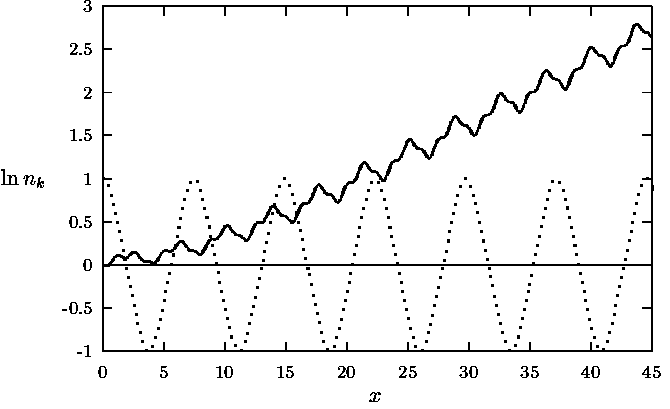
\includegraphics[width=0.6\linewidth, height=0.3\textheight]{Images/Chap4/ConformalTheory_Fig3}
	\caption{The typical resonant production of particles at the particular choice of rescaled comoving momentum $ \kappa^{2}=1.6 $, and the parameter $ \frac{g^{2}}{\lambda}=3 $. This plot shows the logarithm of the comoving particle number density $ n_{k} $. The number of particles grows exponentially with $ \log n_{k} \simeq 2\mu_{k}x$. In this case, $\mu_{k}\simeq 0.035 $ \cite{Chap4:ModelLambdaPhi4Reference}.}
	\label{fig:conformaltheoryfig3}
\end{figure}



\subsection*{Solution for $ \frac{g^{2}}{\lambda} \ll 1 $}
Considering that the function $ f(x) $ can be expanded in series (\ref{Chap4:lambdaPhi4_EllipticCosineForm}), comes out that the leading contribution to $ X_{k}(x) $ comes from the lower harmonic $ \cos(4\pi x/T) $. Keeping only this term, the equation for $ X_{k} $ can be reduced to the Mathieu equation
\begin{equation}
\label{Chap4:lambdaPhi4_MathieuEquationCase}
\frac{d^{2}X_{k}}{d\tau^{2}} + (A+2q\cos 2\tau)X_{k}=0,
\end{equation}
where $ \tau=2\pi x/T $, $ A=(T\kappa/2\pi)^{2} $ and $ q=0.4973\ \frac{g^{2}}{2\lambda}\ (\frac{T}{2\pi})^{2} $. Thus, for $ \frac{g^{2}}{\lambda} \ll 1 $ the parametric resonance corresponds to that of the Mathieu equation. 

The exponentially growing solution has the maximum characteristic exponent
\begin{equation}
\mu_{max} \simeq 0.1467 \Bigg(\frac{g^{2}}{\lambda}\Bigg).
\end{equation}
\begin{figure}[h]
	\centering
	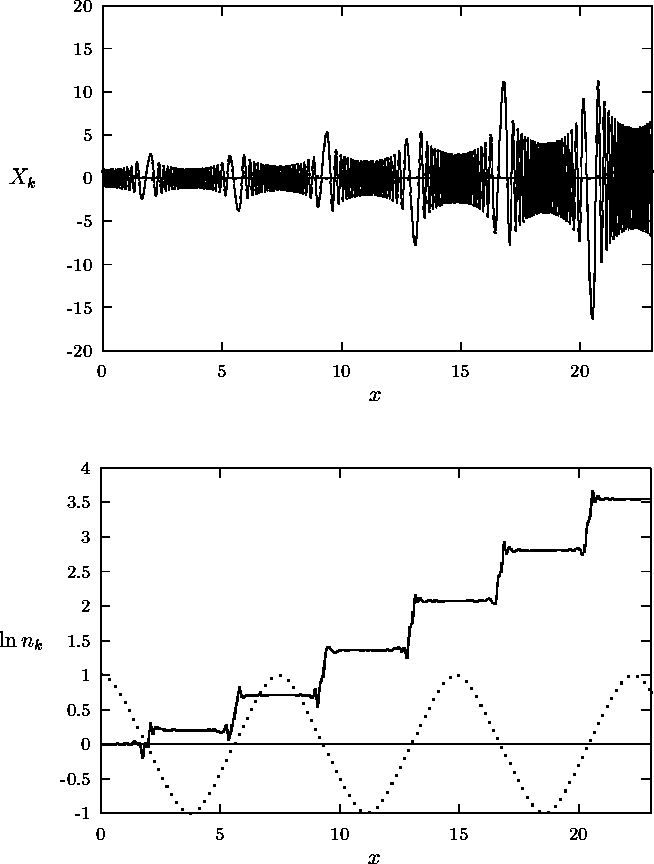
\includegraphics[width=0.6\linewidth, height=0.45\textheight]{Images/Chap4/ConformalTheory_Fig7}
	\caption{The upper plot shows the time-dependence of the real part of the eigenmode $ X_{k}(x) $, which demostrates the adiabatic (semiclassical) beheaviour between zeros of the inflaton oscillations (dotted line), where the comoving occupation number $ n_{k} $ of created particles is constant (lower plot). The lower plot shows $\log n_{k}$ as a function of time $ x $. Particle creation occurs in a step-like manner only in the vicinity of the zeros of the inflaton field, where the adiabaticity is broken. This beheaviour is the same of the quadratic potential model of the previous sections. In this plot the characteristic exponent $ \mu_{k}\simeq 0.1 $, $ \frac{g^{2}}{\lambda}=5050 $ and $\kappa^{2}=29$ \cite{Chap4:ModelLambdaPhi4Reference}.}
	\label{fig:conformaltheoryfig7}
\end{figure}

\subsection*{Solution for  $ \frac{g^{2}}{\lambda} \gg 1 $ }
In this case the parameter $ \frac{g^{2}}{\lambda}$ is very large. We report in (Fig. \ref{fig:conformaltheoryfig7}) from \cite{Chap4:ModelLambdaPhi4Reference} the plot of the time evolution of the fluctuations $ X_{k}(x) $ and the comoving number of particles in a given mode, $ n_{k}(x) $.

In this case, the evolution is similar to the broad/stochastic resonance regime in quadratic potential model. For $ \frac{g^{2}}{\lambda} \gg 1 $, the evolution of the modes $ X_{k}(x) $ is adiabatic and the number of particles $ n_{k}(x) $ is constant between the zeros of the background field. The number density of particles changes only near times $ x=x_{j} $,  when the amplitude of the oscillating inflaton field crosses zero $ (\varphi(x=x_{j})=0) $. We can use, as for the quadratic potential model, the scattering potential method.

We assume that the semiclassical solution is valid everywhere but around $ x_{j} $. Thus, away from the points $ x_{j} $, the mode function $ X_{k}(x) $ is adiabatic and we consider the scattering in the parabolic potential $ (x-x_{j})^{2} $ at the moment $ x_{j} $ between the incoming waves (for $ x<x_{j} $) and the outgoing waves (for $ x > x_{j} $). In the vicinity of $ x_{j} $ we have $ cn(x,1/\sqrt{2})\simeq (x-x_{j}) $, and from (\ref{Chap4:lambdaPhi4_fluctuations}) we obtain the simple equation
\begin{equation}
\label{Chap4:lambdaPhi4_simpleEquationAroundXj}
\frac{d^{2}X_{k}}{dx^{2}} + \Bigg(\kappa^{2} + \frac{g^{2}}{2\lambda}(x-x_{j})^{2}\Bigg) X_{k}= 0.
\end{equation}
In this way we can solve this equation in terms of coefficients  for transmissivity and reflectivity (see \cite{Chap4:ModelLambdaPhi4Reference} for details).

From \cite{Chap4:ModelLambdaPhi4Reference } turns out that in this case
\begin{equation}
\label{Chap4:lambdaPhi4_umaxParabolicPotential}
\mu_{max} = \frac{2}{T}\ln(1+\sqrt{2}) \simeq 0.2377.
\end{equation}
This is a general result for the upper limit of $ \mu_{max} $ for an arbitrary $ g^{2}/\lambda $. Therefore, in this special case the resonance is stronger both in terms of the characteristic exponent $ \mu_{max} $ and the width $ \kappa^{2} $.
\subsection{End of resonance}
We can study the end of the resonance with the pure $ \frac{1}{4}\lambda\phi^{4} $ model, with $ g^{2}=0 $ and no $\chi$-field involved. Indeed, if one neglects backreaction, the equations describing the resonance for the modes $\phi_{k}$ coincide with the equations for the modes $\chi_{k}$ in the theory $ g^{2}=3\lambda $ (see the equations (\ref{Chap4:lambdaPhi4_EquationChi}) and (\ref{Chap4:lambdaPhi4_EquationPhik}). Therefore, it is sufficient to study the theory with $ g^{2}=3\lambda $.

The main reason for the termination of the resonance in the $ \frac{1}{4}\lambda \phi^{4} $ model is the restructuring of the resonance band due to the backreaction of created particles. Indeed, it is sufficient to shift the position of the resonance band in momentum space by few percent to stop the growing of the leading resonant mode $\phi_{k}$.
There are two effects that lead to the restructuring of the resonance band. First, particle production reduces the energy  of the scalar field, and therefore reduces the amplitude of its oscillations. This means that the oscillations reduce their frequency and the resonance band is moved towards smaller $ k $. On the other hand, the effective mass of the field $\varphi$ grows due to its interaction with the $\phi$-particles. We then have an increase of the frequency of oscillations and a shift of the resonance band towards larger $ k $. Therefore, these effects act in opposite direction. 
From computer simulations of \cite{Chap4:ModelLambdaPhi4Reference} in this theory results that efficient preheating ends as soon as the fluctuations of produced particles $ \langle \varphi^{2}\rangle  $ grow to $ 0.05\ \tilde{\phi}^{2} $.

The  resonance in the particular case  of the pure theory $ \lambda\phi^{4} $ is inefficient because the resonance band in this theory is very narrow and the characteristic exponent $\mu$ is extremely small. However, when we take into account also the $\chi$-field with $ g^{2}=\lambda $ or $ g^{2}=2\lambda $ the characteristic exponent is much greater and the resonance band is very broad. It is much more difficult to shut down the resonance in such theories.

In the next subsection we discuss the case in which the conformally invariance is broken by a small mass term.

\subsection{Preheating with a massive self-interacting inflaton}
In the previous sections we investigated parametric resonance in the theory $ \frac{m^{2}}{2}\phi^{2} + \frac{g^{2}}{2}\phi^{2}\chi^{2} $. In this theory reheating can be efficient only if $ g\Phi \gg m $, with $\Phi$ the amplitude of the oscillating inflaton field. Due to the rapidly decrease of the amplitude $\Phi$, the parameter $ q $ in the Mathieu equation rapidly changes and we have a stochastic resonance regime.

In the theory $ \frac{\lambda}{4}\phi^{4} + \frac{g^{2}}{2}\phi^{2}\chi^{2} $, instead, the decreasing of the inflaton field $\phi$ does not make the resonance stochastic because all parameters of the resonance scale in the same way as $\Phi$ due to the conformal invariance.

However, neither of these two theories is completely general. Indeed, in the theory of the massive scalar field we expects terms $\sim \lambda \phi^{4}$ because of radiative corrections. On the other hand, in many realistic theories the effective potential is quadratic with respect to $\phi$ near the minimum of the effective potential. Therefore, one can study the general theory  $\frac{m^{2}}{2}\phi^{2} + \frac{g^{2}}{2}\phi^{2}\chi^{2} +\frac{1}{4} \lambda \phi^{4} $. We report here in (Fig. \ref{fig:conformaltheoryfig9}) the plot of \cite{Chap4:ModelLambdaPhi4Reference}, in which are shown the development of the resonance both for the massless theory, and for a theory with a small $ m $. See the paper for details. In the purely massless theory the logarithm of the number density $ n_{k} $ for the leading growing mode increases linearly. Instead, in the case with a small mass $ m $ the resonance becomes stochastic. However, in the case with smaller $ g^{2}/\lambda $  and a little massive inflaton field, the resonance is not stochastic, but it may consist of stages of regular resonance separated by stages without any resonance. Therefore, the presence of a little mass term can modify the nature of the resonance even if this term is much smaller than $ \lambda \phi^{4} $.

In this model if the ratio of $ g/\sqrt{\lambda} $ is smaller than a certain critical value, $ \sqrt{\lambda}M_{pl}/m $, the resonance never become stochastic. Otherwise, if $g/\sqrt{\lambda} > \sqrt{\lambda}M_{pl}/m $, the resonance originally develops as in the massless conformal theory and then, with the decrease of $ \Phi(t) $, the resonance becomes stochastic. In all cases the resonance stops when $ \Phi(t) $ becomes sufficiently small. Another interesting model studied in \cite{Chap4:ModelLambdaPhi4Reference} is the case with spontaneous symmetry breaking with the change of sign of $ m^{2} $, i.e.  $V(\phi,\chi)= -\frac{m^{2}}{2}\phi^{2} + \frac{g^{2}}{2}\phi^{2}\chi^{2} +\frac{1}{4} \lambda \phi^{4} $.
\begin{figure}
	\centering
	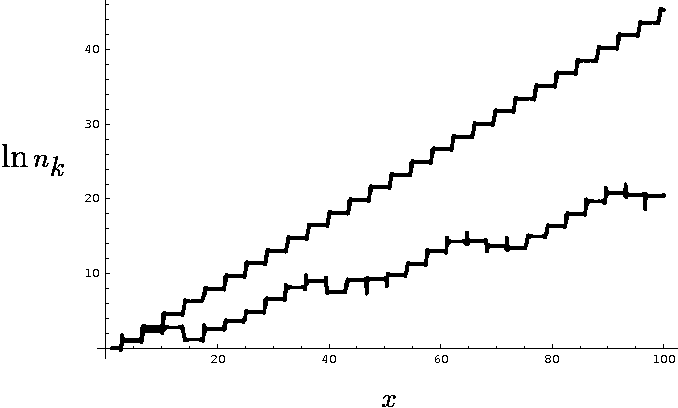
\includegraphics[width=0.6\linewidth, height=0.3\textheight]{Images/Chap4/ConformalTheory_Fig9}
	\caption{Development of the resonance in the theory $ \frac{m^{2}}{2}\phi^{2} + \frac{\lambda}{4}\phi^{4} + \frac{g^{2}}{2}\phi^{2}\chi^{2} $ for $ \frac{g^{2}}{\lambda}=5200 $. The upper curve corresponds to the massless theory, the lower curve describes stochastic resonance  with a theory with a mass $ m $ which is chosen to be much smaller than $ \sqrt{\lambda}\phi $ during the whole period of calculations. Nevertheless, the presence of a small mass term completely changes the development of the resonance \cite{Chap4:ModelLambdaPhi4Reference}.}
	\label{fig:conformaltheoryfig9}
\end{figure}


\section{Tachyonic Preheating}
In the second chapter we considered the hybrid inflation model
\begin{equation}
\label{Chap4:TachyonicPreheating_InflationModel}
V(\phi,\sigma)=\frac{1}{4\lambda}(M^{2}-\lambda\sigma^{2})^{2} + \frac{1}{2}m^{2}\phi^{2} + \frac{1}{2}g^{2}\phi^{2}\sigma^{2},
\end{equation}
where $ m $ and $ M $ are the bare masses of the scalar fields $\phi$ and $\sigma$. At large values of the fields, their effective masses squared are both positive and the potential  has the simmetry $ \sigma \rightarrow -\sigma $. At small values of the field $\phi$, the potential has a maximum at $\phi=\sigma=0$ and a global minimum at $\phi=0$, $\sigma=\sigma_{0} \equiv M/\sqrt{\lambda}$, where the simmetry is broken.

In the second chapter we discussed how inflation proceeds/ends in this model. Motion starts at large $\phi$, where the effective mass of the $\sigma$-field is positive and large. The $\sigma$-field is sitting at the minimum of the potential at $\sigma=0$. During the slow-roll, the effective mass of the $\sigma$-field is $ m^{2}_{\sigma}=g^{2}\phi^{2}-M^{2} $. When the field $\phi$ acquires the critical value $ \phi_{c}=M/g $, fluctuations of the massless $\sigma$ field trigger the symmetry breaking phase transition that ends inflation.

Therefore, in the simplest model of hybrid inflation, inflation ends as soon as the inflaton field decreases below $ \phi_{c}=M/g $. It is important to understand the \textit{waterfall} process in which the $\sigma$ field goes from $ \sigma=0 $ to $ |\sigma|=M/\sqrt{\lambda} $. In fact, considering the classical equation of motion, the field  at $ \sigma = 0 $ cannot change its value because the first derivative of the effective potential vanishes at $ \sigma=0 $. Indeed, in this case the process of SSB occurs due to the exponential growth of quantum fluctuations. The trigger field $\sigma$ acquires a negative mass squared $ -\mu^{2}(\phi)=g^{2}(\phi^{2}-\phi_{c}^{2}) $, which vanishes at the critical point, but becomes large and grows up to $ \mu(0)=M $ as the field $\phi$ moves to $\phi=0$.

Quantum fluctuations of the trigger field $\sigma$ with momentum \textbf{k} grow as $\sim e^{\omega_{k} t}$, where $\omega_{k}=\sqrt{\mu^{2}-k^{2}}$, $ k=|\textbf{k}| $.  Therefore, simmetry breaking occurs due to the growth of fluctuations with $ k\langle \mu $. We obtain an inhomogeneous distribution of the field $\sigma$ with $ \langle \sigma\rangle =0 $. The resulting distribution of the field $\sigma$ is rather homogeneous on a scale $ l\sim \mu^{-1} $ because the rate of exponential growth is maximal at $ k=0 $, and the fluctuations with $ k>\mu $ do not grow (see \cite{Chap4:TachyonicPreheating}).

After inflation, the fields oscillate around their minima producing particles. In this model there are two fundamental frequencies of oscillations near the minimum of the effective potential: $ m_{\sigma}=\sqrt{2}M $ and $ m_{\phi}=gM/\sqrt{\lambda} $. We have also two different scales for the fields $\phi$ and $\sigma$: $ \phi_{c}=M/g $ and $\sigma_{0}=M/\sqrt{\lambda}$.

In the case $\lambda \gg g^{2}$ we have $ \sigma_{0}\ll\phi_{0} $ and $ m_{\sigma} \gg m_{\phi} $. In this case oscillations of the $\sigma$-field tend to be insignificant and most of the energy of these two fields is concentrated in the oscillations of the inflaton field $\phi$. On the other hand, for $\lambda \ll g^{2}$ we have $ m_{\sigma} \ll m_{\phi} $. In this case we have the opposite situation: oscillations of the inflaton field $\phi$ is insignificant and most of the energy of the two fields will be concentrated in the oscillations of the scalar field $\sigma$. Finally,  the case $ \lambda \sim g^{2} $ is much more complicated. Both fields will oscillate with a comparable amplitude, transferring energy to each other in a chaotic way.

In \cite{Chap4:TachyonicPreheating} are studied different cases deriving, for each situation, the Mathieu equation that describes the system. For example, are studied the case in which  $g^{2} \ll \lambda$, where the beheaviour of the inflaton $\phi$ dominates, or the opposite case,  $g^{2} \gg \lambda$. However, if we consider the amplitude of oscillations of the field $\sigma$ small, resonance occurs in the narrow resonance regime and then, in general, the production of particles is inefficient in all cases . Instead, considering $ M \gg H $ for $ \lambda \ll g^{2} $, we obtain a different result. In this type of model we have a quick end of inflation and a large amplitude of oscillations of the field $\sigma$ after inflation. The field makes $ 10^{6} $ oscillations before the amplitude is damped by the expansion of the universe (taking for example a model with $ g=1$, $\lambda=10^{-2}$, $ m=10^{3} GeV $ and $ M=1.3 \times 10^{11} $ GeV, it gives $ H \sim 2\times 10^{4}$ GeV, $ m_{\phi} \sim 5 \times 10^{7} H $ and $ m_{\sigma} \sim 8 \times 10^{6} H $ ). 
As a result, we obtain very efficient production of $\sigma$ and $\phi$ particles. In the plots (Fig. \ref{fig:tachyonicmodel}) from \cite{Chap4:TachyonicPreheating} are shown the growth of the fluctuations for the two fields neglecting backreaction. Preheating in this model is so efficient that it completes within few oscillations.

The efficiency in this model of the process of production of $\sigma$-particles can be explained by the tachyonic instability of the field in the first stages of its rolling down. Neglecting the expansion of the universe, fluctuations of the field $\sigma$ in the beginning of the process grow as $\exp \sqrt{k^{2}-M^{2}t}$. The value of the homogeneous field $ \langle \sigma\rangle  $ vanishes at all time and all the energy is stored in the fluctuations of the $\sigma$-field.

Various simulations  are computed about this stage. We will see in the next chapter that preheating process after hybrid inflation is even more violent  than in the case of parametric resonance that occurs after chaotic inflation. For more details about this model see \cite{Chap4:TachyonicPreheating}.
\begin{figure}
	\centering
	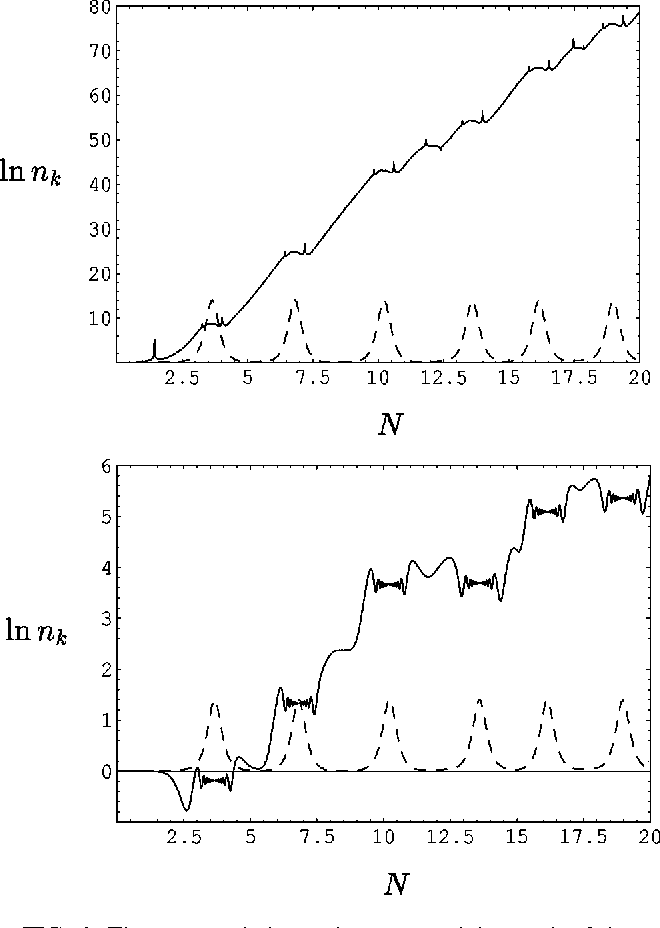
\includegraphics[width=0.6\linewidth, height=0.45\textheight]{Images/Chap4/TachyonicModel}
	\caption{The top panel shows the exponential growth of the occupation number $ n_{k} $ and $\sigma$ particles, as a function of $ N=\bar{m}_{\sigma}t/ 2 \pi $ for $ k=0.43M $ with $ \bar{m}_{\sigma}^{2} \equiv 2M^{2} $. It acquires a typical growth parameter $\mu_{k} \simeq 0.3$ during the last stages of preheating. The lower panel shows the occupation number $ n_{k} $ of $\phi$-particles, for $ k=0.2M $. In this case the growth parameter is an order of magnitude smaller, $\mu_{k} \simeq 0.023$. The dashed line shows the oscillations of the field $\sigma$. The upper panel shows $ 10\sigma/\sigma_{0} $, while the lower panel shows $ \sigma/\sigma_{0}. $ The number of the $\sigma$-field oscillations differs from $ N $ because the oscillations are not armonic. In this model $ \lambda = 10^{-2} $, $ g=1 $, $ m=10^{3} $ GeV, $ M=1.3 \times 10^{11} $ GeV \cite{Chap4:TachyonicPreheating}.}
	\label{fig:tachyonicmodel}
\end{figure}

\section{Other Models}
In this last section we briefly review some other very interesting models of preheating.
\subsection{Instant preheating}
Instant preheating works even in the models where parametric resonance does not develop. It leads to an almost instantaneous reheating accompanied by the production of superheavy particles with masses which may be as great as $ 10^{17}-10^{18} $ GeV \cite{Chap4:InstantPreheating}.

Consider the simple chaotic inflation model with $ \frac{m^{2}}{2}\phi^{2}+ \frac{\lambda}{4}\phi^{4} $ and assume that the inflaton interacts with some other scalar field $\chi$ with the interaction term $ -\frac{1}{2}g^{2}\phi^{2}\chi^{2} $. We have seen in the previous sections that, when the inflaton $\phi=0$, we have a production of $\chi$-particles. This mechanism is described by the broad resonance process. However, concentrate on the first instant of the process. Initially only a small fraction of the energy of the inflaton field is transferred to the particles $\chi$. Suppose that the particles $\chi$ interact with fermions $\psi$ with the coupling $ h\bar{\psi}\psi\chi $. If the coupling with fermions is strong enough, the $\chi$ particles may decay to fermions before the oscillating inflaton field $\phi$ returns back to the minimum of the effective potential. In this way, parametric resonance does not occur, but the total energy of the $\chi$-particles at the moment of their decay is much greater than their energy at the moment of their creation. Indeed, the effective mass of each $\chi$-particle grows as $ m_{\chi}=g\phi $ when the field $\phi$ rolls up from the minimum of the effective potential. We can consider the $\chi$-particles being \textit{fattened} by the energy of the inflaton field. These $\chi$ fattened particles decay to fermions when they have the greatest mass, i.e. when $\phi$ reaches the maximal value.

The $\chi$-particles can decay to two fermions with mass that can be as large as $ 5 \times 10^{17}$ GeV  for $ g \sim 1 $. It results that this mass is two orders of magnitude greater than the masses of the particles that can be produced by the parametric resonance process. The total energy density of the produced particles also becomes two orders of magnitude greater than their energy density at the moment of their production. Therefore, the chain $ \phi \rightarrow \chi \rightarrow \psi  $ significantly enhance the efficiency of the energy transfer from the inflaton field to matter.

Moreover, the produced superheavy particles $\psi$ eventually dominate the energy density of the universe, even if initially their energy density was relatively small. When these particles decay, they eventually lead to the reheating of the universe.

The entire non perturbative process is referred as \textit{instant preheating} since it occurs immediately after the end of inflation within less than one oscillation of the inflaton field (see \cite{Chap4:InstantPreheating} for the complete detailed model).  This process can lead to the production of particles with momenta and masses many orders of magnitude greater than the inflaton mass.

A peculiar and very interesting effect that can happens in this model occurs when the masses of the produced $\chi$ particles, $ m_{\chi}=g|\phi| $, become greater than $ M_{pl} $. When this happens, each $\chi$-particle becomes a Planck-size black hole, which immediately evaporates and reheats the universe.
\subsection{Preheating of fermions}
During preheating the leading channel of particle production is the non-perturbative process of parametric resonance of bosonic fields during which they are produced exponentially. Initially, because of the Pauli principle that prohibits unbounded creation of fermions, it was assumed that the creation of fermions can be treated with perturbation theory for the decay of individual inflatons. However, in \cite{Chap4:FermionPreheating} it is found that we can have preheating of fermions in a regime called $ \textit{parametric excitation of fermions} $. Fermionic preheating differs significantly from the perturbative expectation. In this case the number density of fermions varies periodically with time.

Consider the Dirac equation for a massless quantum Fermi field $\psi(t,\textbf{x})$:
\begin{equation}
\label{Chap4:OtherModels_DiracEquation}
[i\gamma^{\mu}\nabla_{\mu} - h\phi(t)]\psi = 0,
\end{equation}
where $\phi(t)$ should be considered as a coherently oscillating scalar field.

Consider the model $ \frac{1}{4}\lambda \phi^{4} + h\bar{\psi}\phi\psi $. We can do a conformal transformation of the involved fields: $\varphi=a\phi$, $\Psi=a^{3/2}\psi$ and $\tau=\sqrt{\lambda \tilde{\varphi}^{2}}\int dt\  a(t)^{-1}$. Take an auxillary field $ X(\tau,\textbf{x}) $, so that $\Psi$ = [i$\gamma^{\mu}\nabla_{\mu} + h\varphi]X$. It is found that the temporal part of the eigenmode $ X_{k} $ obeys the oscillator-like equation \cite{Chap4:FermionPreheating}
\begin{equation}
\label{Chap4:OtherModels_EquationForFermionEvolution}
\ddot{X_{k}} + \Bigg(\kappa^{2} + qf^{2} - i\sqrt{q}\dot{f}\Bigg)X_{k}=0.
\end{equation}
This is an equation with complex frequency which depends periodically on time. The comoving momentum $ k $ enters the equation in the combination $\kappa^{2}=k^{2}/\lambda\tilde{\varphi}^{2}$. The background oscillation enters in the form $ f(\tau) = cn\Bigg(\tau,\frac{1}{\sqrt{2}}\Bigg) $ with unit amplitude. Finally, the combination of the coupling parameters  $ q=h^{2}/\lambda $ defines the structure of the solution of (\ref{Chap4:OtherModels_EquationForFermionEvolution}). The comoving occupation number of particles $ n_{k} $ in a given spin state is given by
\begin{equation}
\label{Chap4:OtherModels_OccupationNumberFermion}
n_{k(\tau)}=\frac{1}{2} - \frac{\kappa^{2}}{\Omega_{k}}Im\Bigg(X_{k}\dot{X}_{k}^{*}\Bigg) - \frac{\sqrt{q}f}{2\Omega_{k}},
\end{equation}
where $\Omega_{k}=\kappa^{2} + qf(\tau)^{2}$ and $ n_{k}\le 1/2 $. From the numerical analysis in \cite{Chap4:FermionPreheating} comes out that the occupation number exhibits high frequency oscillations, which are modulated by  a long period beheaviour (see (Fig. \ref{fig:fermionicpreheating}) from \cite{Chap4:FermionPreheating}). 

For values $ q \gg 1 $, as in the case of parametric resonance production of bosonic particles, the number of fermions is almost constant between two successive zeros of the inflaton field. It jumps in a step-like manner at instances when $\phi(t)$ crosses zero. In this case we talk about \textit{parametric excitation of fermions} and $ q $ plays the role of the resonance parameter. For details about this model see \cite{Chap4:FermionPreheating}.
\begin{figure}
	\centering
	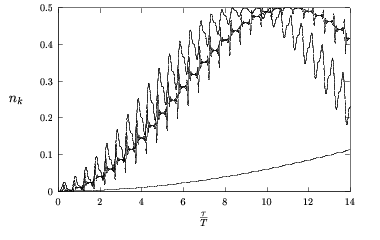
\includegraphics[width=0.7\linewidth, height=0.3\textheight]{Images/Chap4/FermionicPreheating}
	\caption{The occupation number $ n_{k} $ in this model as a function of $ \tau $ in units of $ T\simeq 7.416 $ (the period of the background oscillations) for $ q=10^{-4} $ (lower), 1 (middle on right), and 100 (upper on right) and $ \kappa^{2} = 0.18,\ 1.11, $ and 11.9, respectevely \cite{Chap4:FermionPreheating}.}
	\label{fig:fermionicpreheating}
\end{figure}

\subsection{Gauge-field preheating}
We can consider the possibilty of preheating via the parametric amplification of a massless, $ U(1) $ abelian gauge field. This is a model studied in \cite{Chap4:GaugeFieldPreheating}. 

In this model the inflaton field $\phi$ is coupled to $ U(1) $ gauge field with the action
\begin{equation}
\label{Chap4:OtherModels_GaugeFieldPreheatingAction}
S = \int d^{4}x \sqrt{-g}\Bigg(-\frac{W(\phi)}{4}F_{\mu\nu}F^{\mu\nu} - \frac{1}{2}\partial_{\mu}\phi\partial^{\mu}\phi - V(\phi)\Bigg),
\end{equation}
where $ W(\phi) $ and $ V(\phi) $ are scalar functions which represent the coupling strength and the inflationary potential, respectevely. The potential of the inflaton field is quadratic, $ V(\phi)=\frac{1}{2}m^{2}\phi^{2} $, and the coupling function has the form
\begin{equation}
\label{Chap4:OtherModels_GaugeFieldPotentialCoupling}
W(\phi)=e^{\phi/M},
\end{equation}
where $ M $ is a free parameter which value is near $ m $. As the scalar field decays, the coupling goes to unity and standard electromagnetism is recovered.

From  the analysis of \cite{Chap4:GaugeFieldPreheating} an abelian $ U(1) $, massless, electromagnetic field can be used as a mechanism  by which energy can be moved from the inflaton field into particles. Moreover, this model does not require additional channel of decay or tachyonic instabilities in order to generate the radiation dominated universe after reheating. Once the energy is moved to the gauge field during resonance, there is no movement of energy back to the scalar field that one normally see in other models.

Once the field $\phi$ becomes small, the coupling function term becomes negligible and the energy deposited in the gauge field remains there. In this model then we obtain a method for creating a universe at the end of inflation with a majority of its energy in a gauge field $ A_{\mu} $. At late times the coupling function is close to unity and the standard dynamics of the gauge field, for example electromagnetism, is recovered. 

Another possibility is the case in which the inflaton is charged \cite{Chap4:ChargedInflatonPreheating}. In this case we consider  the inflaton field $\phi$ to be a complex scalar field under an abelian $ U(1) $ symmetry, with the standard kinetic term replaced by 
\begin{equation}
\label{Chap4:OtherModels_U1KineticTemr}
\Delta \mathcal{L} = - |D_{\mu}\phi|^{2} = -|\partial_{\mu}\phi|^{2} + ig(\phi \partial_{\mu}\phi^{*}-\phi^{*}\partial_{\mu}\phi)A^{\mu} + g^{2}|\phi|^{2}A_{\mu}A^{\mu},
\end{equation}
where the final term is similar to the standard preheating interaction $ g^{2}\phi^{2}\chi^{2} $, but with the scalar field $\chi$ replaced by a gauge field. Since spin-1 fields are bosonic, this can leads to significant parametric resonance. 

\subsection{Multi-field preheating}
In the case we consider several oscillating homogeneous fields, the periodicity of the time-dependent background can be violated. Unless special situations \cite{Chap4:Lozanov}, the time-dependent coefficients in the equation of motion governing the fluctuations are not exactly periodic. This can lead a stochastic resonance if the adiabaticity condition is violated. 

In the case in which the number of oscillating homogeneous fields is much greater than one, the effective masses of the daughter fields evolve randomly. This reduces the efficiency of the particle production, but resonance still takes place. It occurs at all wavenumbers, not only within particular resonance bands. In fact, we can consider the condensed matter phenomenon of Anderson localitation, in which small random impurities make eigenfunctions exponentially localized in space (see \cite{Chap4:Lozanov}). Therefore, we expect that in the case of preheating, time-dependent masses with random components give rise to exponentially growing modes at all wavelength. A reference for this type of models can  be found in \cite{Chap4:multifieldPreheating}.

\chapter{Non-linear Evolution}
The study of reheating in the early universe involves the description of the evolution of interacting fields in a dense, high-energy environment.  Preheating and the subsequent phase of Thermalization involve non-perturbative interactions of fields with exponentially large occupation numbers in states far from thermal equilibrium. As seen in the previous chapter, approximation methods like the Hartree approximation fail in the description of the process because they neglect important scattering terms.

The simplest model of preheating involves a chaotic inflationary scenario with potential $ V(\phi)=\frac{1}{2}m^{2}\phi^{2} $ and a quadratic coupling  of the inflaton to another field $ \frac{1}{2}g^{2}\phi^{2}\chi^{2} $. We studied the process of preheating. However, backreaction of inhomogeneous fluctuations quickly brings the system of interacting scalar fields to a strongly non-linear regime characterized  by very high occupation numbers.

Another important class of inflationary models are given by hybrid inflation scenerios. As discussed, preheating in hybrid inflation, which contains a symmetry breaking mechanism, occurs in the tachyonic way and has a very different character respect to the chaotic inflation scenario. 

In this chapter we present the numerical results about the process of non-linear interactions of fields during and after preheating. We consider both tachyonic and chaotic models.

\section{Tachyonic Model}
We start discussing the dynamics of spontaneous symmetry breaking that leads to the tachyonic preheating process. In this model the particle production is extremelly efficient, much more than  parametric resonance models after chaotic inflation. For reference and details see \cite{Chap5:DynamicsSymmetryBreaking} and \cite{Chap5:TachyonicInstability}.

In the simplest models the instability appears because of the presence of a tachyonic mass term such as $ -m^{2}\phi^{2}/2 $ in the effective potential. This implies the exponentially growing of long wavelength quantum fluctuations $\phi_{k}$ of the field $\phi$ with momenta $ k < m $, $\phi_{k} \sim \exp(t\sqrt{m^{2}-k^{2}})$, which leads to spontaneous symmetry breaking.

The spontaneous symmetry breaking process is a strongly non-linear, non-perturbative effect, and leads to  production of particles with large occupation numbers. The approximation methods like perturbative theory or the Hartree approximation completely fail in the description. However, in the past years  methods of lattice simulations have been developed. They are based on the observation that quantum states of bose fields with large occupation numbers can be interpreted as classical waves and their dynamics can be fully analized through lattice simulations of relativistic wave functions. A significant advantage of this method is that the semi-classical nature of these effects allows us to have a clear visual picture of all the processes involved.

To understand the basic features of a SSB model we consider the simplest model 
\begin{equation}
	\label{Chap5:TachyonicModel}
V(\phi)=\frac{\lambda}{4}(\phi^{2}-v^{2})^{2} \equiv -\frac{m^{2}}{2}\phi^{2} + \frac{\lambda}{4}\phi^{4} + \frac{m^{4}}{4\lambda},
\end{equation} 
where $ m^{2}\equiv \lambda v^{2} $ and $\lambda \ll 1$. $ V(\phi) $ has a maximum at $ \phi=0 $ with curvature $ V''=-m^{2} $ and a minimum at $\phi=\pm v$.

Consider the Klein-Gordon equation for the scalar field fluctuations in this model:
\begin{equation}
\label{Chap5:TachyonicModel_KGEquation}
\ddot{\phi}_{k} + (k^{2} + V'')\phi_{k}=0.
\end{equation}
Suppose that initially at $ t=0 $  the mode functions describing quantum fluctuations in the symmetric phase $\phi=0$ are the same as for a massless field, $\phi_{k}=\frac{1}{\sqrt{2k}}e^{-ikt + i \textbf{k}\textbf{x}}$. Then, at $ t=0 $ we turn on the term $ -m^{2}\phi^{2}/2 $ corresponding to the negative mass squared $ -m^{2} $. The modes with $ k = |\textbf{k}| < m  $ grow exponentially, $ \sim e^{t\sqrt{m^{2} - k^{2}}} $, until $ \sqrt{\langle \delta \phi^{2}\rangle } $ reaches the value $\sim v/2$.  At $\phi \sim v/\sqrt{3}$ the curvature of the effective potential vanishes and one has the usual oscillations of all the modes instead of the tachyonic instability. This happens within a time $ t_{*} \sim \frac{1}{2m}\ln \frac{C}{\lambda} $, where $ C\sim 10^{2} $ (see  \cite{Chap5:TachyonicInstability}).

To study this process is convenient to use the occupation number $ n_{k} $ of produced particles. Indeed, in situations where the number of particles is well defined (this happens at the end of the process) the occupation number is an adiabatic invariant, i.e. it does not change during the field oscillations, unless some dramatic changes occur to the system. In the previous chapter we have seen the standard definition of the occupation number, which is valid for $ m^{2} \ge 0 $,
\begin{equation}
\label{Chap5:TachyonicModel_occupationNumber}
n_{k}=\frac{\omega_{k}}{2}\Bigg(\frac{|\dot{\phi}_{k}}{\omega_{k}^{2}} + |\phi_{k}|^{2}\Bigg) - \frac{1}{2}.
\end{equation}
However, this definition should not be interpreted as the occupation number of particles during the tachyonic regime. In fact, during this stage the effective mass squared of the field $\phi$ becomes negative since $\omega_{k} = \sqrt{k^{2} + m^{2}}$ becomes imaginary. We can define a formal quantity using for example $ \sqrt{k^{2} + |m^{2}|} $ in the expression for $ n_{k} $ whenever $ m^{2} < 0 $. This formal quantity $ n_{k} $ can be interpreted  as the occupation number of particles after the end of the tachyonic regime, when $ m^{2} > 0 $. Indeed, these two quantities matches at the end of the tachyonic stage.

 The exponential growth of fluctuations during the tachyonic regime can be interpreted as the growth of the occupation number of particles with $ k \ll m $. Considering the instant $ t_{*} $ at which the tachyonic growth of the fluctuations ends, it is showed in \cite{Chap5:TachyonicInstability} that $ n_{k} $ for $ k \ll m  $ at the time $ t_{*} $ grows up to $ n_{k} \sim \exp(2mt_{*})  \simeq \mathcal{O}(10^{2})\lambda^{-1} \gg 1$. Thus, for small $ \lambda $  fluctuations with $ k \ll m $ acquire very large occupation numbers. Moreover, these fluctuations will have large amplitude  and will be in a squeezed state. If we consider the general solution, it will contains two terms, a growing mode $\sim Ae^{\omega t}$ and a decreasing mode $ \sim Be^{-\omega t} $, but after a short time only the growing mode survives. Then, only modes with $ k < m $ survives after the beginning of the tachyonic regime independently of the initial phase of quantum fluctuations, and their amplitude will become extremely large. This implies that we can study these modes by lattice simulations since we can interpret them as classical waves. 
 
Equation for fluctuations in the model $ V(\phi)=-\frac{m^{2}}{2}\phi^{2} + \frac{\lambda}{4}\phi^{4} + \frac{m^{4}}{4\lambda} $ is 
\begin{equation}
\label{Chap5:equationFluctuation}
\ddot{\phi}_{k} + \Bigg(k^{2} -m^{2} +3\lambda\phi^{2}\Bigg) \phi_{k} = 0.
\end{equation}
This is the Lame equation that we have seen in the previous chapter, and its solutions depend on the parameter combination $ \sqrt{\lambda}\phi_{0}/m  $.
In the numerical computation this equation should be solved together with the equation for the background field $\phi(t)$:
\begin{equation}
\label{Chap5:equationBackground}
\ddot{\phi} - m^{2}\phi + \lambda \phi^{3} = 0.
\end{equation}
In this model the study of the growing of  perturbations is a generalitation of the theory of parametric resonance in the model $ \frac{\lambda}{4}\phi^{4} $, studied using the stability/instability chart of the Lame equation. The additional instability is due to the presence of the negative mass term.

From the analysis of \cite{Chap5:TachyonicInstability} we have the following picture. Consider the evolution of the occupation number $ n_{k} $ of the modes $ \phi_{k}  $ with $ \lambda = 10^{-4} $ and the field rolling from $ \phi_{0}=0.01v $.
Start with a mode $\phi_{k}$ with $ k\ll m $. When the field $\phi$ rolls from $\phi=\phi_{0}$ to $\phi=v/\sqrt{3}$, the occupation number becomes $ \sim e^{9} $. Then, the field reaches the bottom of the effective potential, goes little beyond this point, bounces back and again approaches the tachyonic region $ \phi < v/\sqrt{3} $. The occupation number of particles with $ k \ll m $ does not change much until the field becomes smaller than $ v/\sqrt{3} $.  After this point, however, the comoving number of particles decreases almost to the same value from which the simulation starts. Indeed, this beheaviour is due to the fact that the solution for the fluctuations has two modes, one growing and the other one decaying. Then, when the field bounces, fluctuations either grow or decay depending on the phase with which they re-enter the tachyonic regime. In (Fig. \ref{fig:tachyonicinstabilityfig1}) from \cite{Chap5:TachyonicInstability} is showed the growth of $ n_{k} $ during three consecutive oscillations of the field $\phi$. During each full oscillation the occupation numbers grow $ e^{15} $ times. Therefore, during $ n $ oscillations the occupation numbers grow $ e^{15n} $ times.
\begin{figure}[h]
	\centering
	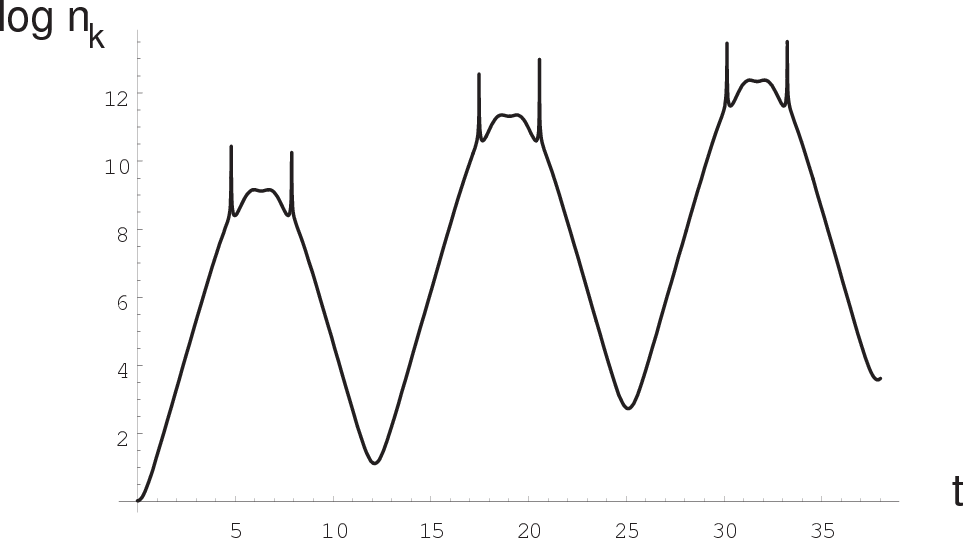
\includegraphics[width=0.6\linewidth, height=0.25\textheight]{Images/Chap5/TachyonicInstability_Fig1}
	\caption{Evolution of the occupation numbers for fluctuations with $ k\ll m $ in the model $ V(\phi)=-\frac{m^{2}}{2}\phi^{2} + \frac{\lambda}{4}\phi^{4} + \frac{m^{4}}{4\lambda} $ \cite{Chap5:TachyonicInstability}.}
	\label{fig:tachyonicinstabilityfig1}
\end{figure}
\begin{figure}[h]
	\centering
	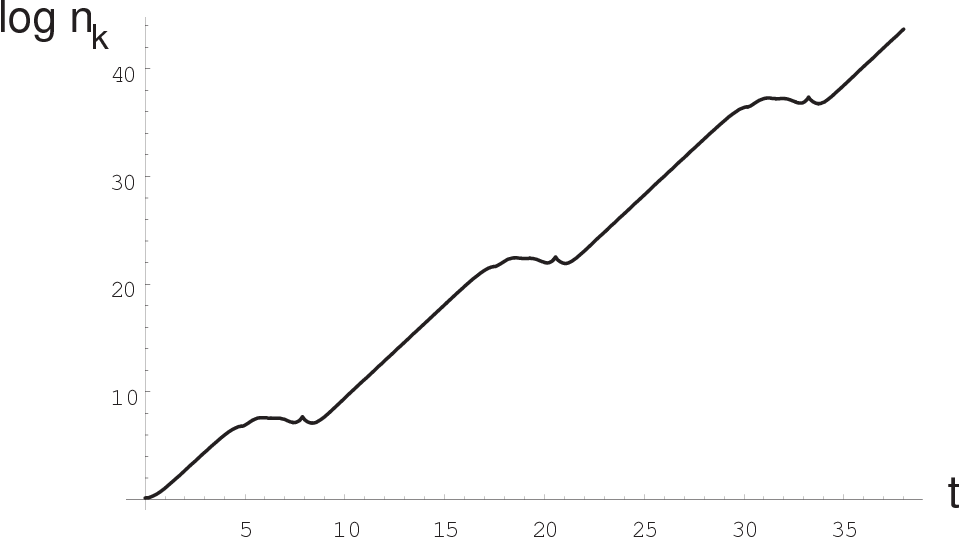
\includegraphics[width=0.6\linewidth, height=0.25\textheight]{Images/Chap5/TachyonicInstability_Fig2}
	\caption{Same as in (Fig. \ref{fig:tachyonicinstabilityfig1}) but for $ k=0.5\ m $\cite{Chap5:TachyonicInstability}.}
	\label{fig:tachyonicinstabilityfig2}
\end{figure}
We obtain from this model then an incredible fast growth, much faster than in the parametric resonance theories with $ m^{2} > 0 $. This process  can rapidly convert all the energy of the homogeneous field into the energy of the classical interacting fields.

If we consider in general a theory with $ V(\phi) \sim -\phi^{n} $ with $ n > 2 $, the growth of the occupation numbers for small $ k $ occurs faster. Indeed, the tachyonic fluctuations with small momenta in the long time limit grow as $\phi_{k} \sim \phi^{n/2}$. 
We can easily prove this statement. Consider a generic model
\begin{equation}
\label{Chap5:PotentialGeneric}
V(\phi)=V_{0}-\lambda\phi^{n}/2.
\end{equation}
Consider the field $\phi$ that begins rolling down from $\phi_{0}$. From energy conservation we have 
\begin{equation}
\label{Chao5:energyConservation}
\frac{1}{2}\dot{\phi}^{2} - \frac{1}{2}\dot{\phi}^{2}_{0} = V(\phi_{0}) - V(\phi).
\end{equation}
 Assume for semplicity that the field starts from $ \phi=0 $ with zero total energy, i.e. $ \phi_{0}=V_{0}=0 $. Then, we have 
 \begin{equation}
\label{Chap5:equationFieldFluctuation}
\frac{1}{2}\dot{\phi}^{2}=-V(\phi) = \frac{1}{2} \lambda\phi^{n},
 \end{equation}
that yields
\begin{equation}
\dot{\phi}=\sqrt{\lambda}\phi^{n/2},
\end{equation}
and finally,
\begin{equation}
\label{Chap5:dependenceFluctuationPotential}
\phi_{k}=C\phi^{n/2}.
\end{equation}
In particular, this implies that in the theory with the potential 
$ -\phi^{2} $ the long wavelength fluctuations grow just like the field itself, i.e. $ \phi_{k} \sim \phi $. If we consider for example a theory with a potential $\sim -\phi^{3} $, the fluctuations grow faster, $ \phi_{k} \sim \phi^{3/2} $, and for the theory $ -\phi^{4} $ they grow even faster, $ \phi_{k} \sim \phi^{2} $.

In the theory $ -m^{2}\phi^{2}$ the fluctuations grow as fast as the scalar field. For example, if one consider $ \phi_{0} \sim 10^{-2}v $, quantum fluctuations grow almost $ 10^{4} $ times when the field falls down from $ \phi=\phi_{0} $ and returns back. The amplitude of inhomogeneites after the return becomes approximately three orders of magnitude larger than $\phi_{0}$. This means that the homogeneous inflaton condensate becomes completely destroyed. When the inflaton field falls down to the minimum of the effective potential again, it becomes divided into large colliding waves. If we consider a general potential  $V(\phi) \sim -\phi^{n} $ with $ n>2 $, the process occurs even more faster (see \cite{Chap5:TachyonicInstability}).

\subsection{Lattice simulations}
To study the beheaviour of this process with lattice simulations in \cite{Chap5:TachyonicInstability} is considered the probability distribution function $ P(\phi,t) $, which is the fraction of the volume containing the field $\phi$ at a time $ t $. At $ t=0 $, at the start of the simulation, the probability distribution is concentrated near $\phi=0$.

In the beginning, quantum fluctuations are very small and the probability distribution $ P(\phi,t) $ is very narrowly focused near $\phi=0$. Then, it spreads out and shows two maxima that oscillate about $\phi = \pm v$ with an amplitude much smaller than $ v $. The symmetry becomes broken within a single oscillation of the distribution of the field $\phi$. After the SSB, the space becomes divided into domains with the field $\phi \sim \pm v$ (see (Fig. \ref{fig:tachyonicinstabilityfig3}) from \cite{Chap5:TachyonicInstability}). The size of the domains is large and they become even larger since large domains eat the small ones. In the numerical analysis  are considered only the modes with $ k < m $, since only these modes experience exponential growth and beheave as classical fields.

\begin{figure}[h]
	\centering
	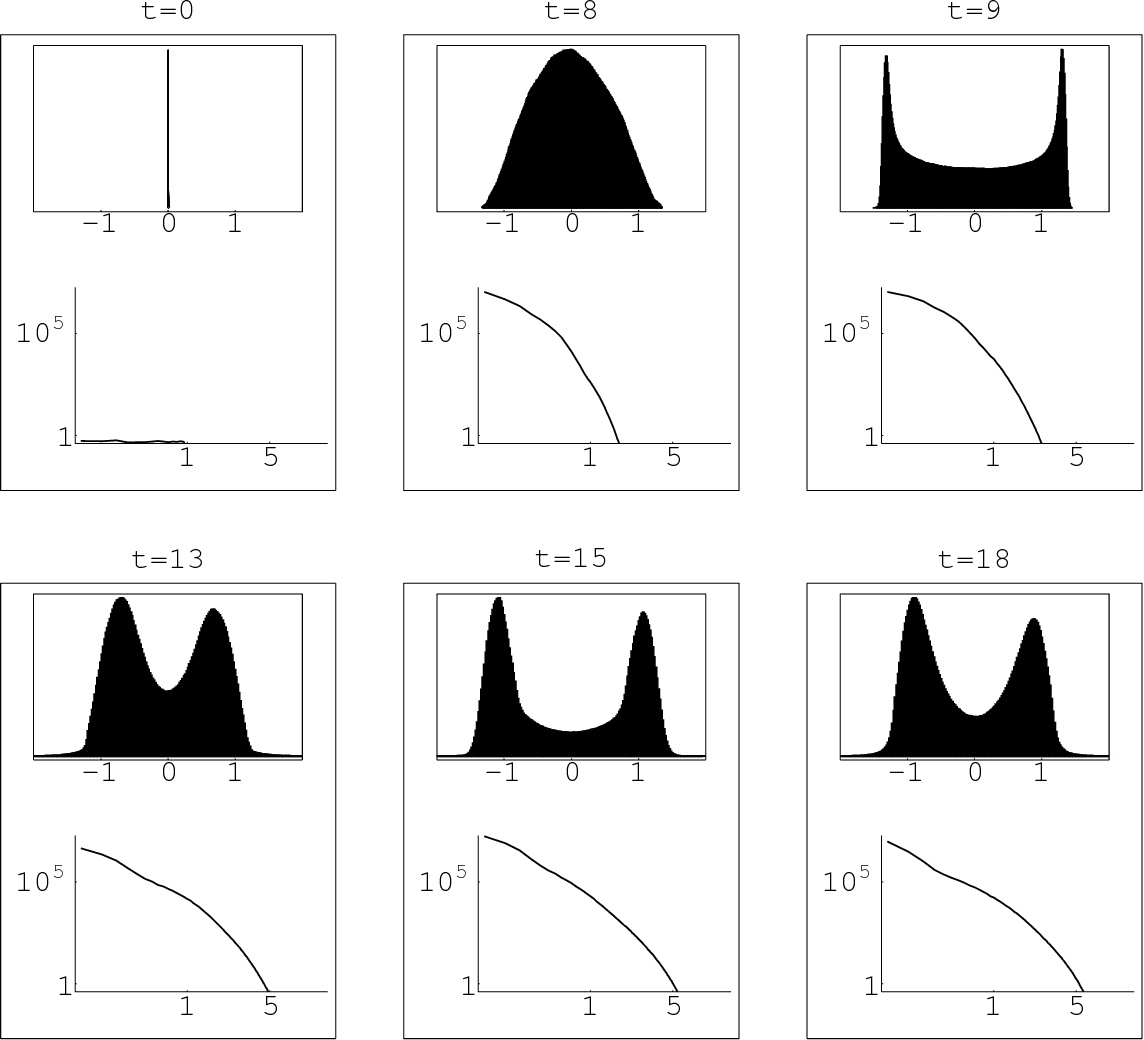
\includegraphics[width=0.7\linewidth, height=0.35\textheight]{Images/Chap5/TachyonicInstability_Fig3}
	\caption{The process of symmetry breaking in the model (\ref{Chap5:TachyonicModel}) for $\lambda = 10^{-4}$. The values of the field are shown in units of $ v $, time is shown in units of $ m^{-1} $. For each moment of time, it is also shown the occupation numbers $ n_{k} $ (the lower part of each panel), with $ k $ measured in units of $ m $. At $ t=0 $ one has $ n_{k}=0 $, as in the usual quantum field theory vacuum. In the beginning of the process the occupation numbers $ n_{k} $ grow exponentially for $ k < m $ ($ k < 1 $ in the figure), but then this growth spreads to $ k>m $ because of domain wall formation and collisions of classical waves of the field $\phi$. Within a single oscillation the occupation numbers for $ k\ll m $ grow up to $\sim 10^{6}$.  The spectrum rapidly stabilizes, but it is not thermal yet, and the occupation numbers remain extremely large \cite{Chap5:TachyonicInstability}.}
	\label{fig:tachyonicinstabilityfig3}
\end{figure}
\begin{figure}
	\centering
	\includegraphics[width=0.7\linewidth, height=0.45\textheight]{Images/Chap5/TachyonicInstability_Fig4}
	\caption{Tachyonic growth of quantum fluctuations and the early stages of domain formation in the simplest theory of spontaneous symmetry breaking with $ V(\phi)=-\frac{m^{2}}{2}\phi^{2} + \frac{\lambda}{4}\phi^{4}$ \cite{Chap5:TachyonicInstability}.}
	\label{fig:tachyonicinstabilityfig4}
\end{figure}
\begin{figure}
	\centering
	\includegraphics[width=0.7\linewidth, height=0.35\textheight]{Images/Chap5/TachyonicInstability_Fig5}
	\caption{Formation of domains in the process of symmetry breaking in the model (\ref{Chap5:TachyonicModel}) \cite{Chap5:TachyonicInstability}.}
	\label{fig:tachyonicinstabilityfig5}
\end{figure}
In (Fig. \ref{fig:tachyonicinstabilityfig4}) and (Fig. \ref{fig:tachyonicinstabilityfig5}) from \cite{Chap5:TachyonicInstability} is showed the growth of fluctuations in a two-dimensional slice of 3D space. Maxima corresponds to domain with $\phi > 0$, while minima correspond to domains with $\phi < 0$. The third image correspond to the first one half of an oscillation. In this moment, the universe is already divided into domains with $ \phi \pm v $ and initial  size somewhat greater than $ m^{-1} $. Inside  each domain the deviation from $ \phi = |v| $ is much smaller than $ v $. Therefore, from the lattice simulation we see that SSB occurs within a single oscillation. Gradually, the size of each domain grows and the domain wall structure becomes more and more stable. If one continues the simulation for a much longer time, we see  formation and growth of domains with $ \phi=\pm v $. In the beginning these domains are small, but they eat each other and grow.

We show also in (Fig. \ref{fig:tachyonicinstabilityfig7}) from \cite{Chap5:TachyonicInstability} the case in which we have the SSB for a theory of a multicomponent scalar field $ \phi_{i} $ with the potential
\begin{equation}
	\label{Chap5:TachyonicModelComplex}
	V(\phi)=\frac{\lambda}{4}(|\phi|^{2}-v^{2})^{2} \equiv -\frac{m^{2}}{2}|\phi|^{2} + \frac{\lambda}{4}|\phi|^{4} + \frac{m^{4}}{4\lambda}.
\end{equation} 
In the plots of (Fig. \ref{fig:tachyonicinstabilityfig7}) is illustrated the dynamics with a two-component scalar field $\phi = (\phi_{1} + i\phi_{2})/\sqrt{2}$. It shows the probability distributions $ P(\phi_{i},t) $ which is the fraction of the volume containing the field $\phi$ at a time $ t $.

In the beginning,  the probability distribution is concentrated near $\phi=0$. Then, it spreads out and stabilizes at $ |\phi|\sim v $ after a single oscillation, which corresponds to SSB. In (Fig. \ref{fig:tachyonicinstabilityfig8}) from \cite{Chap5:TachyonicInstability} is showed the occupation numbers $ n_{k} $ of produced particles. During the first oscillation the occupation numbers grow up to $ 10^{7}-10^{8} $ for $ k < m $ ($ k < 1 $ in the figure). Then, the occupation numbers at $ k < m $ slightly decrease, while at $ k > m $ begin to grow. In the model of a complex scalar field, instead of domain walls, we obtain strings that are produced when the field falls down. We report in (Fig. \ref{fig:tachyonicinstabilityfig9}) from \cite{Chap5:TachyonicInstability} a simulation of the strings produced after one half of an oscillation of the complex scalar field. The whole process of string formation in this model occurs within a single oscillation.

We see that, as in the case of the one-component scalar field, we obtain a formation of topological defects from the SSB. Indeed, this is not a small correction but an important feature of SSB. Topological defects, like other inhomogeneities generated by tachyonic instability, drain the energy of the scalar field rolling down to the minimum of the effective potential. In this way, they diminuish the amplitude of subsequent oscillations of the inflaton field.
\begin{figure}
	\centering
	\includegraphics[width=0.6\linewidth, height=0.4\textheight]{Images/Chap5/TachyonicInstability_Fig7}
	\caption{The process of symmetry breaking in the model (\ref{Chap5:TachyonicModelComplex}) for a complex field $ \phi=\frac{1}{\sqrt{2}}(\phi_{1} + i\phi_{2}) $ \cite{Chap5:TachyonicInstability}.}
	\label{fig:tachyonicinstabilityfig7}
\end{figure}
\begin{figure}
	\centering
	\includegraphics[width=0.5\linewidth, height=0.25\textheight]{Images/Chap5/TachyonicInstability_Fig8}
	\caption{Occupation numbers $ n_{k} $ of particles produced during tachyonic preheating in the model of a complex scalar field $\phi$ with effective potential $ V(\phi)=-m^{2}|\phi|^{2} + \lambda|\phi|^{4} $ with $\lambda = 10^{-4}$. In the beginning  (lower curves), $ n_{k} $ grows for $ k\le m $ ($ k\le 1 $ in this figure), but then eventually this growth spreads to larger $ k $ \cite{Chap5:TachyonicInstability}.}
	\label{fig:tachyonicinstabilityfig8}
\end{figure}
\begin{figure}
	\centering
	\includegraphics[width=0.6\linewidth, height=0.35\textheight]{Images/Chap5/TachyonicInstability_Fig9}
	\caption{Strings produced after one half of an oscillation in the model (\ref{Chap5:TachyonicModelComplex}) for a complex field $\phi$ \cite{Chap5:TachyonicInstability}.}
	\label{fig:tachyonicinstabilityfig9}
\end{figure}
\subsection{Tachyonic model simulations}
An important example of tachyonic model is provided by the theory
\begin{equation}
	\label{Chap5:TachyonicModel1}
V(\phi)=-\frac{\lambda}{3}v\phi^{3} + \frac{\lambda}{4}\phi^{4} + \frac{\lambda}{12}v^{4}.
\end{equation}
This potential is a prototype of the potential that appears in descriptions of symmetry breaking in F-term hybrid inflation \cite{Chap5:FTerm}. In this model the fluctuations increase considerably if the initial amplitude is somewhat greater than $ \delta \phi_{c} \sim \frac{\lambda v}{4\pi^{2}} $. Low probability fluctuations with $ \delta \phi \gg \delta \phi_{c} $ correspond to peaks of the initial Gaussian distribution of the fluctuations  of the field $\phi$ (see \cite{Chap5:TachyonicInstability}). In this model of tachyonic preheating the whole process looks not like a uniform growth of all modes, but more like bubble  production. The numerical simulation is showed in (Fig. \ref{fig:tachyonicinstabilityfig12}) from \cite{Chap5:TachyonicInstability}. The bubbles, that are high peaks of the field distribution, grow, change shape, and interact with each other, rapidly dissipating the vacuum energy $ V(0) $. In (Fig. \ref{fig:tachyonicinstabilityfig14}) is showed the occupation numbers of produced particles with $ \lambda=10^{-2} $. These occupation numbers grow up to $ 10^{4}-10^{5} $ within a single oscillation.

\begin{figure}
	\centering
	\includegraphics[width=0.7\linewidth, height=0.5\textheight]{Images/Chap5/TachyonicInstability_Fig12}
	\caption{Field values on a 2D slice through the lattice for $ V=-\frac{\lambda}{3}v\phi^{3} + \frac{\lambda}{4}\phi^{4} $. The growth of quantum fluctuations of $\phi$ looks like bubble formation. The bubbles expand and collide even before the average field value reaches the minimum. Preheating occurs due to a combined effect of bubble production, tachyonic instability and bubble wall collisions \cite{Chap5:TachyonicInstability}.}
	\label{fig:tachyonicinstabilityfig12}
\end{figure}
\begin{figure}
	\centering
	\includegraphics[width=0.6\linewidth, height=0.25\textheight]{Images/Chap5/TachyonicInstability_Fig14}
	\caption{Occupation numbers of particles produced during tachyonic preheating in the model (\ref{Chap5:TachyonicModel1}) with $\lambda = 10^{-2}$ \cite{Chap5:TachyonicInstability}.}
	\label{fig:tachyonicinstabilityfig14}
\end{figure}
We consider now the model of tachyonic preheating with potential
\begin{equation}
\label{Chap5:TachyonicPreheatingPotential}
V(\phi,\sigma)=\frac{\lambda}{4}(|\sigma|^{2}-v^{2})^{2} + \frac{g^{2}}{2}\phi^{2}|\sigma|^{2} + \frac{1}{2}m^{2}\phi^{2},
\end{equation}
that we have seen in the previous chapter. If $\sigma$ is a real one-component scalar, the SSB may lead to the formation of domain walls. In this case, assuming $\sigma$ a complex field, SSB after inflation produces cosmic strings \cite{Chap5:DynamicsSymmetryBreaking}. 

\begin{figure}
	\centering
	\includegraphics[width=0.6\linewidth, height=0.4\textheight]{Images/Chap5/SymmetryBreaking_Fig7}
	\caption{Snapshots of the growth of the Higgs peak in a full non-linear lattice simulations, for $ \lambda=0.11/4 $ and $ V=0.003 $. Plotted is the value of the Higgs amplitude $\sigma$ in the $(x,y) $ plane, where the $ z $-coordinate is that of the highest peak. Note that several peaks appear in the simulation. Here are showned the first stages of the evolution, where the highest peak invaginates and form the bubble. In the figure $\phi$ is the our Higgs field $\sigma$ \cite{Chap5:FalseVacuumDecay}.}
	\label{fig:symmetrybreakingfig7}
\end{figure}
\begin{figure}
	\centering
	\includegraphics[width=0.6\linewidth, height=0.4\textheight]{Images/Chap5/SymmetryBreaking_Fig8}
	\caption{Same as in (Fig. \ref{fig:symmetrybreakingfig8}). Here are showed the late stages, in which gradients arise from collisions of bubbles and the symmetry is broken. In the figure $\phi$ is the our Higgs field $\sigma$ \cite{Chap5:FalseVacuumDecay}.}
	\label{fig:symmetrybreakingfig8}
\end{figure}
In this model a lattice simulation can be found in \cite{Chap5:FalseVacuumDecay} and it is showed in (Fig. \ref{fig:symmetrybreakingfig7}) and (Fig. \ref{fig:symmetrybreakingfig8}).  This model leads, as the previous one, to bubbles formation. The non-perturbative evolution is studied numerically solving the coupled classical equations of motion for the inflaton field $\phi$ and the Higgs field $\sigma$ with gaussian initial conditions. 
As seen in the other models, also in this one SSB in not at all a homogeneous process. Already in the linear regime, the Higgs field $\sigma$ evolves by developing lumps in space that grows with time. In the plots (Fig. \ref{fig:symmetrybreakingfig7})  and (Fig. \ref{fig:symmetrybreakingfig8}) from \cite{Chap5:FalseVacuumDecay} is followed the classical evolution of the Higgs' lumps. From the figure we can see that the peak of the largest  Higgs' lump is the first to break the symmetry, i.e. to reach $ |\sigma|=v $, and soon after the center of the lump invaginates, creating an approximately spherically symmetric \textit{bubble}, with ridges that remain above $ |\sigma|=v $. Finally, from these plots we see that neighbouring bubbles collide and the symmetry gets fully broken through the generation of higher momentum modes.

Regarding the beheaviour of the $ |\sigma(\textbf{x},t)| $ at the center of the highest Higgs lump, it oscillates around $ |\sigma|=v $ with an amplitude that is dumped in time. Oscillations of the field remain coherent and give rise to concentric bubbles, until the time when bubble collisions break the symmetry.

\section{Chaotic Models}
Consider the potential of chaotic inflation
\begin{equation}
\label{Chap5:ChaoticModel_potential}
V(\phi,	\chi)= \frac{1}{2}m^{2}\phi^{2} + \frac{1}{2}g^{2}\phi^{2}\chi^{2},
\end{equation}
where $\phi$ is the inflaton and $\chi$ the scalar field coupled to it. At the end of inflation, $\phi$ is a homogeneous oscillating field and $\chi$ a quantum field which obeys an oscillator equation with a periodic frequency $ \omega_{k}^{2}=\frac{k^{2}}{a^{2}} + g^{2}\phi^{2} $. In the previous chapter we have seen that the amplitude $\chi_{k}(t)$ undergoes parametric resonance, leading to large occupation numbers of created particles $ n_{k} $. Since the occupation numbers grow very fast, we can treat the field $\chi(t,\textbf{x})$ as a classical scalar field. Once the $\chi$ field is amplified in this way, the other fields coupled to it are themselves amplified. Thus, within a short time of linear preheating (of order dozens of inflaton oscillations), fluctuations of $\chi$ generate inhomogeneous fluctuations of the inflaton field $\phi$.

 The equation of motion for $\phi$
\begin{equation}
\label{Chap5:EquationForPhi}
\Box\phi + m^{2}\phi^{2} + g^{2}\chi^{2}\phi = 0,
\end{equation}
in Fourier space reads
\begin{equation}
\label{Chap5:EquationForPhiFourierSpace}
\ddot{\phi}_{k} + 3H\dot{\phi}_{k} + ((k^{2}/a^{2}) + m^{2})\phi_{k} = g^{2}\phi_{0}(t) \int d^{3}q\chi_{q}\chi_{q}^{*},
\end{equation}
where is neglected the term that is third order with respect to fluctuations and $\phi_{0}(t)$ is the background oscillation \cite{Chap5:Fragmentation}. When the amplitudes of the fields $\phi$ and $\chi$ become sufficiently large we obtain a full non-linear problem. The field evolution can be well determined using the classical equation of motion (\ref{Chap5:EquationForPhi}) supplemented by the equation for the field $\chi$,
\begin{equation}
\label{	Chap5:ChaoticModelEquationForChi}
\Box \chi + g^{2}\phi^{2}\chi=0.
\end{equation}
To obtain the simulations in this section of non-linear preheating it is used the program LATTICEEASY \cite{Chap5:Latticeeasy}. LATTICEEASY can generally solve the classical equations of motion for interacting scalar fields, with or without the effects of the expansion of the universe. This program has a variety of applications since it simulates the nonlinear scalar field dynamics, i.e. parametric resonance, formation of gravitational waves, phase transitions, formation of topological defects, Thermalization after preheating. Each particular scalar field potential that the program solves is encoded in a model file, which is read in LATTICEEASY. The model contains all the necessary equations for running the potential and includes the potential itself and its first and second derivatives, all of which have to be provided in the model file. The model contains also all the parameters for a given run of the program, the number of grid points, the time step, and a number of other general variables specific to each run.

 LATTICEASY uses a staggered leapfrog algorithm with a fixed time step. This means that at each step the field values $ f $ and their derivatives $\dot{f}$ are stored at two different times $ t $ and $ t + dt/2 $, respectevely. The derivatives are used to advance the field values by a full step $ dt $, and then the field values are used to calculate the second derivatives $\ddot{f}$, which are in turn used to advance the field derivatives by $ dt$ (see \cite{Chap5:Latticeeasy}).
 
 \begin{figure}
 	\centering
 	\includegraphics[width=0.8\linewidth, height=0.3\textheight]{Images/Chap5/Fragmentation_Fig1}
 	\caption{Evolution of spectra in the combination $ k^{3}\omega_{k}n_{k} $ of the $\phi$ and $\chi$ fields during and immediately after preheating. Bluer plots show later spectra. Horizontal axis $ k $ is in units of $ m $ \cite{Chap5:Fragmentation}.}
 	\label{fig:fragmentationfig1}
 \end{figure}
 \begin{figure}
 	\centering
 	\includegraphics[width=0.7\linewidth, height=0.3\textheight]{Images/Chap5/Fragmentation_Fig2}
 	\caption{Evolution of the comoving number density of $\phi$ (red, lower plot) and $\chi$ (blue, upper ploat) in units of $ m^{3} $. Time is in units of $ 1/m $ \cite{Chap5:Fragmentation}.}
 	\label{fig:fragmentationfig2}
 \end{figure}
For chaotic inflation we show the results of \cite{Chap5:Fragmentation} in (Fig. \ref{fig:fragmentationfig1}) expressed in terms of the evolution of the occupation numbers $ n_{k}(t) $ with $ m=10^{-6} M_{pl} $ (fixed by CMB normalitation) and $ g^{2}=2.5 \times 10^{-7} $. The size of the simulation box is $ L=10m^{-1} $ and the grid contains $ 256^{3} $ points. The spectra in (Fig. \ref{fig:fragmentationfig1})  show a rapid growth of the occupation numbers of both fields, with a resonant peak that develops first in the infrared ($ k\simeq k_{*} $), and then moves towards the ultraviolet as a result of rescattering. In the other plot in (Fig. \ref{fig:fragmentationfig2}) from \cite{Chap5:Fragmentation} is showed the evolution of the comoving number density for the fields $\phi$ and $\chi$. We can see clearly the exponentially fast growing of the occupation number of the field $\chi$, due to parametric resonance, followed by even faster growth of the field $\phi$ due to the interaction. This beheaviour is in accordance with (\ref{Chap5:EquationForPhiFourierSpace}).

Another feature of preheating is the onset of chaos: small differences in the initial conditions for the fields lead to exponentially divergent solutions, i.e. $D(t) \simeq e^{\lambda t} $, where $ D $ is the distance in phase space between the solutions and $\lambda$ is called Lyapunov exponent (see \cite{Chap5:Fragmentation}). After the violent transition, the distance $ D $ begins to diverge exponentially towards the turbolent stage.

The evolution of the fields in configuration space is showed in (Fig. \ref{fig:fragmentationfig4}) from \cite{Chap5:Fragmentation}. Each frame shows the spatial profile of the fields $\phi$ and $\chi$ along a two-dimensional slice of the 3D lattice. Times are reported in units of $ 1/m $.

\begin{figure}[h]
	\centering
	\includegraphics[width=0.75\linewidth, height=0.6\textheight]{Images/Chap5/Fragmentation_Fig4}
	\caption{Values of the $\phi$ and $\chi$ fields in a two dimensional slice through the lattice. The horizontal axes are spatial axes and the vertical axis is field value \cite{Chap5:Fragmentation}.}
	\label{fig:fragmentationfig4}
\end{figure}
\begin{figure}[h]
	\centering
	\includegraphics[width=0.6\linewidth, height=0.5\textheight]{Images/Chap5/Fragmentation_Fig6}
	\caption{Field distributions. The horizontal axes are field values and the vertical axis represents the frequency of that field value on the lattice. The black dots represent the simulation results and the red lines are best-fit Gaussian curves. The fitting lines can not be seen in the first frame  because they lie directly under the dots \cite{Chap5:Fragmentation}.}
	\label{fig:fragmentationfig6}
\end{figure}
For $ t \le 100 $, we have the initial evolution of the fields characterized by linear growth of fluctuations of $\chi$. The positive and negative peaks correspond to the peaks  of the initial gaussian random field $\chi$. During this stage the fluctuations have the form of a superposition of standing waves with random phases, which yield to a random gaussian field. The first panel in (Fig. \ref{fig:fragmentationfig4}) shows the fields at the end of this first linear stage. After this point, the oscillations become nonlinear and $\phi$ becomes excited. The amplitude of these $\phi$ oscillations grows much faster than the initial $\chi$ oscillations, and the oscillations have different and changing frequencies.

For $ t \le 110 $, the peaks reach their maximum amplitude, comparable to the initial value of the homogeneous field $\phi$, and begin to spread. The two lower left panels of (Fig. \ref{fig:fragmentationfig4})  shows the peaks expanding and colliding.

By $ t=124 $, the fluctuations have spread throughout the lattice. Shortly after this time all coherence is lost and the field configurations appear to be like random turbolence.

The evolution during the non-linear period is analyzed not using the Fourier-mode description (\ref{Chap5:EquationForPhiFourierSpace}), but instead considering the configuration space description (\ref{Chap5:EquationForPhi}).

We show also in (Fig. \ref{fig:fragmentationfig6}) from \cite{Chap5:Fragmentation} the evolution of the statistics of the fields $\phi$ and $\chi$. In (Fig. \ref{fig:fragmentationfig6})  are showed the field distributions, i.e. histograms, at various times during the evolution. Initially both fields have gaussian distributions from their random quantum fluctuations. The field $\phi$ is sharply peaked around $\phi_{0}$, and the field $\chi$ is centered around zero. As non-linear effects become important, the statistics of the two fields become complicate. The distribution  of the inflaton field becomes at times sharply peaked to one side (when the condensate is at an extreme end of its oscillation), and at other times with a presence of the homogeneous component plus a significant inhomogeneous component, i.e. bi-modal. The statistics of the field $\chi$ also becomes strongly non-gaussian. Moreover, the statistics of the two fields remain non-gaussian for a long time after preheating. At $ t=300 $, when the simulation in \cite{Chap5:Fragmentation} ends, the fields are still non-gaussian.

The picture that emerges in this model is similar to what we observed in the previous section for tachyonic preheating in hybrid inflation.  For example, in the model (\ref{Chap5:TachyonicModel1}) small initial random fluctuations of $\phi$ are amplified by the non-linear $\phi^{3}$ term. The peaks of the gaussian field then begin to grow very fast relatively to the surrounding regions of $\phi$. In the same way, in the model discussed in this section, it is found in \cite{Chap5:Fragmentation} that oscillations of the fields $\chi$ and $\phi$ grow initially at the locations of the peaks in the initial $\chi$ field. In this model these growing peaks form a pattern of standing waves that persists throughout the linear regime, and then begin to spread and overlap as rescattering becomes important.

Therefore, we can split the reheating process from the end of inflation, when we have the inflaton condensate, to the begin of the radiation era, where we have the radiation of randomly moving waves, in four stages. The first is the exponentially growing of small inhomogeneities that emerge from vacuum fluctuations (due to parametric resonance or tachyonic instabilities). During this stage fluctuations are linear and the fields are gaussian random fields. The second stage is violent backreaction and rescattering of the waves with non-gaussian, non-linear and non-thermal fluctuations. In the next chapter we will study the third and the last stage of reheating. The third stage is the Kolmogorov turbolence. During this phase, the fluctuations are nearly gaussian and energy gradually cascades towards high momentum modes. The final stage is Thermalization where eventually the fields reach thermal equilibrium characterized only by the temperature.

To end this section, we discuss an important signature from the non-linear bubble-stage of inflaton fragmentation. Lumps of the scalar fields correspond to large energy density inhomogeneites at the scale of those bubbles, say $ R $. The collisions of bubbles generate gravitational waves. The fraction of the total energy at the time of preheating converted into gravitational waves is significant. To estimate this quantity we consider the following result. The energy converted into gravitational waves from the collision of two black holes is of the order of the black hole masses. Suppose the mass of lumps of size $ R $ equals to a fraction $ f $ of a black hole of the same size.
Thus, the fraction of energy converted to gravitational waves from the collision of two lumps is $ f $. Scalar field lumps at the Hubble scale would form black holes, so $ f = (RH)^{2} $. We can then estimate the fraction of the total energy  converted into gravitational waves as
\begin{equation}
\label{Chap5:fractionTotalEnergyGW}
\frac{\rho_{GW}}{\rho_{rad}} \simeq (RH)^{2}.
\end{equation}
The present-day frequency of this gravitational radiation is  estimated as 
\begin{equation}
\label{Chap5:frequencyGW}
f\simeq \frac{10^{7} GeV}{M} Hz,
\end{equation}
where $ M=V^{1/4} $ is the energy scale of inflation with the potential $ V $.\\
For the chaotic inflation model in this section the size of the bubbles is $ R\sim few/m $ and they begin colliding at $ H\sim m/100 $ \cite{Chap5:Fragmentation}. Then, the fraction of energy converted into gravitational waves is estimated as $\sim 10^{-3}-10^{-4}$. For chaotic inflation with $ M  $ at the GUT scale this frequency is too short and not observable. However, better possibility of observations comes from low energy hybrid inflation where $ f $ can be much smaller. 

Gravitational waves continue to  be generated during the turbolent stage and even during thermal equilibrium due to thermal fluctuations, but with a smaller amplitude. In the final chapter of this thesis we present various numerical simulations of gravitational wave production from preheating after chaotic and hybrid inflation.


\section{Oscillons}
We end this chapter considering a very peculiar model from which we can have a signature in the spectrum of gravitational waves. 

Many interesting non-perturbative phenomena may take place during preheating such as formations of oscillons when we have the inflaton fragmentation. Oscillons are spatially localized, temporally oscillating configurations of a nonlinear scalar field. They are first described by Bogolubsky and Makhankov \cite{Chap5:Oscillon}, and then are studied in great detail through numerical simulations. 

Oscillons are not strictly stable, even in the classical limit since they are not associated  with conserved charges, but are long-lived (see \cite{Chap5:OscillonAfterInflation} and \cite{Chap5:Oscillon_OscillonFormationInThreeDimension}. There are various models in which massive oscillons are generated during preheating, and in a large class of inflationary scenarios oscillons may account for the majority of the energy density in the post-inflationary universe, i.e. axion monodromy model. In these scenarios, the universe undergoes a transient matter-dominated phase.

Oscillons can form in a variety of models. However, an oscillon-dominated universe  can follow inflation driven by a single-field model. Oscillons can form if the inflaton potential is
\begin{equation}
	\label{Chap5:Oscillons_Potential}
	V(\phi)=\frac{1}{2}m^{2}\phi^{2} + U(\phi),
\end{equation}
where $ U(0)=0 $ and $ U(\phi) < 0 $ for some range of $\phi$.

Consider potentials with $ V(\phi) \sim \phi^{2\alpha} $ during inflation and $\alpha < 1$. These models are generated by various string and supergravity scenarios which yield $ U(\phi) < 0  $ at large $\phi$. It is also required that $ V(\phi) $ has a stable minimum set at the origin in order to have $ V(\phi) \sim \phi^{2} $ at small $\phi$. We can consider the potential
\begin{equation}
\label{Chap5:OscillonsPotential}
V(\phi)=\frac{m^{2}M^{2}}{2\alpha}\Bigg[\Bigg(1+\frac{\phi^{2}}{M^{2}}\Bigg)^{\alpha} - 1\Bigg],
\end{equation}
where $ 0 \le \alpha \le 0.9$ and $ M \le 0.05 M_{pl} $. In particular, $\alpha = 1/2$ is the axion monodromy model. When $\phi/M$ is small, we have $ V(\phi) \simeq m^{2}\phi^{2}/2 $. For this potential very massive oscillons can be copiously produced after inflation, giving rise to an oscillon-dominated phase. They eventually decay reheating the universe.

A very interesting feature of this model is the production of gravitational waves as a consequence of an oscillon-dominated phase in the early universe. Gravitational waves can arise during their formation, during the oscillon dominated phase  itself, and during their decay and the subsequent Thermalization of the universe \cite{Chap5:GWFromOscillon}. In \cite{Chap5:GWFromOscillon} is computed the gravitational wave spectrum during the resonance and the oscillon-formation phase. In (Fig. \ref{fig:oscillonsfig2}) from \cite{Chap5:GWFromOscillon} is showed the resulting spectrum. The spectrum has a specific and characteristic structure, with multiple peaks and troughs.

In models in which the scalar field is complex, one can also get nontopological solitons, called Q-balls \cite{Chap5:QBall}. Also Q-balls can generate high-frequency gravitational waves \cite{Chap5:QBallGWS}.
\begin{figure}
	\centering
	\includegraphics[width=0.6\linewidth, height=0.35\textheight]{Images/Chap5/Oscillons_Fig1}
	\caption{Sample output from a 3D oscillon simulation. Contours delineate regions where the local energy density exceeds the average value by a factor 10, showing localized, approximatevely spherical, overdensities characteristic of oscillons \cite{Chap5:Oscillon_OscillonFormationInThreeDimension}.}
	\label{fig:oscillonsfig1}
\end{figure}
\begin{figure}
	\centering
	\includegraphics[width=0.6\linewidth, height=0.35\textheight]{Images/Chap5/Oscillons_Fig2}
	\caption{Peaks and troughs of the gravitational wave spectrum. The vertical lines correspond to the gravitational wave frequencies associated with the different harmonics of the oscillon \cite{Chap5:GWFromOscillon}.}
	\label{fig:oscillonsfig2}
\end{figure}


\chapter{Thermalization}
We have seen in the previous chapters that after inflation all energy density is stored in a Bose-condensate, the coherently oscillating inflaton field. This stage is highly unstable: non-adiabatic processes as parametric resonance or tachyonic instability lead to an explosive and fast  decay of the inflaton and production of particles. The decay of the inflaton leads to a rapid amplification of one or more bosonic fields to exponentially large occupation numbers. This process eventually shuts down because of backreaction and rescattering. We obtain  at the end a turbolent medium of coupled, inhomogeneous, classical waves far from equilibrium.

The transition from this stage of turbolence to a hot Friedmann universe in thermal equilibrium is the stage called Thermalization. A theory of Thermalization of the fields is necessary to bridge inflation and the Hot Big Bang universe. The details of  Thermalization depend on the costituents of the fundamental Lagrangian and their coupling. At first glance the description of this process would be strongly model-dependent. However, from various analysis, i.e. \cite{Chap6:DevelopmentEquilibrium}, many features of this stage seem to hold generically across a wide spectrum of models. This is due to the fact that the conditions at the end of preheating are in general not qualitatevely sensitive to the details of inflation.

In this chapter we review the main common features of Thermalization among various different models. We will discuss the beheaviour of the spectrum in terms of the so-called Kolmogorov turbolence.

\section{Rules of thermalization}
In \cite{Chap6:DevelopmentEquilibrium} is calculated the evolution of  the number density $ n(t) $ of particles with time for different models. For all models examinated in the paper,  $ n(t) $  shows an exponential growth during preheating. This exponential growth is well-studied in the previous chapters and corresponds to the explosive particle production due to parametric resonance or tachyonic instabilities. After preheating, the fields enter a turbolent regime during which $ n(t) $ decreases. Indeed, the decrease can be interpreted as a consequence of the particle interactions: as $ n_{k} $ shifts from low to high momenta the overall number decreases. We then have a flow towards infrared momenta.

This beheaviour can be understood from (Fig. \ref{fig:developmentofequilibriumfig2}) from \cite{Chap6:DevelopmentEquilibrium}. The spectrum shows a cutoff at some momentum $ k_{*} $, above which the occupation number falls off exponentially.  This is because we have an excess of occupation numbers at low $ k $ due to parametric resonance. Indeed, parametric resonance is typically most efficient at exciting low momentum modes, and becomes completely inefficient above a certain cutoff $ k_{*} $. From (Fig. \ref{fig:developmentofequilibriumfig2}) we can see the flow towards higher momenta. The ultraviolet cutoff is initially at the momentum $ k_{*} $, where parametric resonance shuts down. However, during the time the cutoff moves to higher $ k $ as more modes are brought into the quasi-equilibrium of the infrared part of the spectrum. Moreover, the infrared sector  gradually flattens as the system approaches a true thermal distribution.

We have an other interesting feature  studied in \cite{Chap6:DevelopmentEquilibrium}. Consider the pure one-field model $ \lambda \phi^{4} $ and the two-field model $ g^{2}\phi^{2}\chi^{2} $. The numerical analysis in \cite{Chap6:DevelopmentEquilibrium} shows that in the first case $ n_{\phi} $ decreases very slowly compared to the second. This occurs because  the interactions between $\phi$ and $\chi$ greatly speed up the Thermalization of both fields (see the plots in \cite{Chap6:DevelopmentEquilibrium}). In the pure $ \lambda \phi^{4} $ model, $\phi$ can only thermalize through its weak self-interaction. Moreover, the spectra of the two fields $\phi$ and $\chi$ are essentially identical and results $ n_{\phi} \simeq n_{\chi} $. The two spectra match shortly after preheating, and from that they evolve identically. This is due to the fact that the potential term $ V\simeq g^{2}\phi^{2}\chi^{2} $ is symmetric with respect to the two fields, and then they act as a single effective field.

Finally, we can also include an additional decay channel for $\chi$. The interaction between $\chi$ and the decay field, $\sigma$, drag $\sigma$ exponentially quickly into an excited state. The field $\sigma$ is exponentially amplified not by parametric resonance, but by its stimulated interactions with the amplified $\chi$-field. The interaction of the two fields does not affect the preheating of $\chi$. From this, results that $ n_{\chi} $ decreases as $\sigma$ grows, so the spectra of $\chi$ and $\phi$ are no longer identical.

\begin{figure}
	\centering
	\includegraphics[width=0.6\linewidth, height=0.25\textheight]{Images/Chap6/DevelopmentOfEquilibrium_fig2}
	\caption{Evolution of the spectrum of the field $\chi$ in the model $ V=\frac{1}{4}\lambda \phi^{4} + \frac{1}{2}g^{2}\phi^{2}\chi^{2}. $The lower plots all show early times. In the bundle of plots higher up the spectrum rises on the right and falls on the left as time progresses  \cite{Chap6:DevelopmentEquilibrium}. }
	\label{fig:developmentofequilibriumfig2}
\end{figure}
In \cite{Chap6:DevelopmentEquilibrium} the previous features are encoutered in various models.  Thus, in the paper are established a set of rules that seem to hold generically. They are called \textit{rules of Thermalization}. We report them in the following:
\begin{enumerate}
	\item \textit{In most models of inflation exist a mechanism for exponentially amplifying fluctuations of at least one field $\chi$. These mechanisms tend to give rise an highly infrared spectrum due to the long-wavelength excitations.}
	
	Indeed, we have seen in the case of single-field models the parametric resonance mechanism. In hybrid models the same amplification is mainly leaded by tachyonic instabilities. Adding additional fields or self-couplings has little or no effect on the resonant period. Moreover, the qualitative features of the fields arising from these processes are largely independent of the details of inflation or the mechanisms used to produce the fields.
	
	\item \textit{Exciting one field $\chi$ is sufficient to rapidly drag all other light fields with which $\chi$ interacts into a similarly excited state}. 
	
	In the paper is simulated the beheaviour of multiple fields directly coupled to $\chi$. It is sufficient to have one field rapidly excited to amplify an entire sector of interacting fields. These  amplified fields will inherit the basic features of the $\chi$-field, i.e. they will have spectra with more energy in the infrared than would be expected for a thermal distribution.
	
	\item \textit{The excited fields will be grouped into subsets with identical characteristic (spectra, occupation numbers, effective temperatures) depending on the coupling strengths.}
	
	In general, fields  that are interacting in a group will thermalize much more quickly than other fields. 
	
	\item \textit{Once the fields are amplified, they will approach thermal equilibrium by scattering energy into higher momentum modes.}
	
	In this process we obtain a slow redestribution of the particle occupation number as low momentum particles are scattered and combined into higher momentum modes. The tilt of the infrared part of the spectrum decreases, meanwhile the ultraviolet cutoff of the spectrum increases. Within each field group the evolution proceeds identically for all the fields. However, different groups can thermalize at very different rates.
\end{enumerate}


\section{Kolmogorov Turbolence}
Turbolence appears in a large variety of non-equilibrium phenomena in nature. In particular, Kolmogorov turbolence was first applied in the study of fluids with large Reynolds number. In this case Kolmogorov identified turbolence as a statistically scale invariant flow of spectral energy mediated by vortex interaction. The same structure may appear in systems of coupled waves \cite{Chap6:turbolence}.

If there exists an active (stationary) source of energy in momentum space, the turbolence is called \textit{stationary} (or driven). When the source is switched off after the stage of activity, the freely propagating energy flux is called \textit{free} turbolence.

In the case of reheating, we can think the inflaton field as a source of energy localized in the infrared part of the spectrum. The energy flows towards a significantly separated region of ultraviolet, high momentum modes. In the first stage of turbolence the energy is pumped out by the zero-mode of the inflaton field. At this stage we have stationary turbolence driven by the zero-mode. The stage of stationary turbolence terminates when the energy left out by the inflaton zero-mode becomes smaller than the energy stored in created particles. From this moment the transport of energy from the source is negligible, and we observe non-stationary evolution of particles distribution towards thermal equilibrium. This last stage of free turbolence is very long and analitically can be described as self-similar evolution.

We can consider first the simple $ \lambda \phi^{4} $ model. In  (Fig. \ref{fig:turbolentThermalizationfig2}) from \cite{Chap6:TurbolentThermalization} we see the exponential growth with time of the occupation numbers, which are shown at different moments of conformal time $\eta$.  $\bar{\phi}_{0}$ denotes the amplitude of the zero-mode oscillations. At the time $\eta = 100$ we have the parametric resonance. At later times, the growth of the resonance peak is stopped by re-scattering of particles out of the resonance band, which leads the appearance of multiple peaks at $ \eta=400 $. At even later times, the spectra becomes smooth because of rescattering.

The particles with small momenta are distributed according to a power-law. At larger momenta  we have a cutoff that moves with time to the ultraviolet. In the system energy is continuosly inputted in the region of $ k $ near the resonance peak. We have a continuos flux of energy across momentum space, from low to high momenta.

We have the following features for $\eta > 1500$ \cite{Chap6:TurbolentThermalization}:
\begin{enumerate}
	\item The system overall is statistically close to a Gaussian distribution of field amplitudes.
	
	\item The spectra in the dinamically important region can be described by a power-law, $ k^{-s} $, with $ s \simeq 3/2 $. The exponent of particle distributions in the power region corresponds to Kolmogorov turbolence. The system is not in thermal equilibrium, which would imply $ s=1 $.
	
	\item the power-law is followed by a cutoff at higher $ k $. The position of the cutoff monotonously grows towards the ultraviolet, reflecting the evolution towards thermal equilibrium.
	
	\item This motion can be described as a self-similar evolution
	\begin{equation}
	\label{Chap6:selfSimilarEvolution}
	n(k,\tau)=\tau^{-q}n_{0}(k\tau^{-p}),
	\end{equation}
where $ \tau = \eta/\eta_{c} $ and $ \eta_{c} $ is some arbitrary late-time moment. In (Fig. \ref{fig:turbolentThermalizationfig3}) from \cite{Chap6:TurbolentThermalization} is reported the best numerical fit of \cite{Chap6:TurbolentThermalization} that correponds to $ q \simeq 3.5p $ and $ p\simeq 1.5 $. The value of the exponent $ p $ determines the rate with which the system approaches equilibrium.
\end{enumerate}
In (Fig. \ref{fig:turbolentThermalizationfig1}) from \cite{Chap6:TurbolentThermalization} is reported the squared amplitude of oscillations of the zero-mode of the inflaton field, $ \phi_{0}=\langle \phi\rangle  $, and the variance $ var(\phi)=\langle \phi^{2}\rangle  -\  \phi_{0}^{2} $, as a function of time. From the plot we can see the initial fast transfer of the zero-mode energy into fluctuations during  preheating (up to $\eta \sim 300$), and the subsequent decreasing of the amplitude of the zero-mode oscillations.

\begin{figure}
	\centering
	\includegraphics[width=0.55\linewidth, height=0.3\textheight]{Images/Chap6/TurbolentThermalization_fig2}
	\caption{Occupation numbers as function of $ k/\bar{\phi}_{0} $ at the conformal time $ \eta=100, 400, 2500,  5000, 10000 $ \cite{Chap6:TurbolentThermalization}.}
	\label{fig:turbolentThermalizationfig2}
\end{figure}
\begin{figure}
	\centering
	\includegraphics[width=0.6\linewidth, height=0.3\textheight]{Images/Chap6/TurbolentThermalization_fig3}
	\caption{On the right hand side, it is plotted the wave energy per decade found in lattice integration at $\eta$=3600,5100,7000,10000. On the left hand size are the same graphs but transformed according to the relation inverse to (\ref{Chap6:selfSimilarEvolution}) \cite{Chap6:TurbolentThermalization}. }
	\label{fig:turbolentThermalizationfig3}
\end{figure}
\begin{figure}
	\centering
	\includegraphics[width=0.6\linewidth, height=0.3\textheight]{Images/Chap6/TurbolentThermalization_fig1}
	\caption{Squared amplitude of the zero-mode oscillations, $\bar{\phi}_{0}^{2}$, and variance of the field fluctuations as functions of time $\eta$ \cite{Chap6:TurbolentThermalization}.}
	\label{fig:turbolentThermalizationfig1}
\end{figure}

\subsection{Analytical model}
In the Kolmogorov turbolence we have a stationary transport of some conserved quantity between different scales in momentum space. Turbolence occurs when a source of energy or particles is present and is localized in some momentum region $ k_{in} $. Considering reheating, the localized source of energy is represented by the coherently oscillating inflaton zero-mode that pumps energy into the system of particles at $ k_{in}\simeq k_{res} $. The mechanism behind the pumping can be parametric resonance, tachyonic instabilities etc.

A complete analytical model is described in \cite{Chap6:TurbolentThermalization} and here we discuss only the main points. The model is based on the analysis of the wave kinetic equation
\begin{equation}
\label{Chap6:waveKineticEquation}
\dot{n}_{k}=I_{k}[n],
\end{equation}
where $ n_{k} $ is the occupation number which describes the average volume of phase space occupied  by the oscillations of a single mode with a wave-number $ k $. The evolution of $ n_{k} $ is a result of wave interactions. The quantity $ I_{k}[n] $ is the collision integral, which is a function of the external momentum $ k $ and a functional of the distribution function $ n $. Considering for example the scattering of two particles into two particles, the collision integral reads
\begin{equation}
\label{Chap6:ColisionIntegral}
I_{k}[n] = \int d\Omega(k,q_{i})F(k,q_{i}).
\end{equation}
In this definition are separated the contributions which are due to the (fixed) particle model, $ d\Omega(k,q_{i}) $, from those which are due to the evolving particle distribution functions, $ F(k,q_{i}) $. In this equation $ k $ is the external momentum and $ q_{i} $ refer to momenta over which the integration is carried out. The infinitesimal solid angle, $ d\Omega(k,q_{i}) $, reads
\begin{equation}
\label{Chap6:solidAngle}
d\Omega(k,q_{i}) = \frac{(2\pi)^{4}|M|^{2}}{2\omega_{k}}\delta^{4}(k_{\mu},q_{i\mu})\prod_{i=1}^{3}\frac{d^{3}q_{i}}{2\omega_{i}(2\pi)^{3}}.
\end{equation}
In this formula the $ \delta $- function represents the usual energy-momentum conservation, $ |M|^{2} $ is the squared matrix element of the process and $\omega_{k}$ is the particle energy.
Finally, $ F $ accounts for quantum effects and, in the limit $ n\gg 1 $, reads in this case
\begin{equation}
\label{Chap6:quantumEffectsf}
F(k,q_{i}) = (n_{k} + n_{q_{1}})n_{q_{2}}n_{q_{3}} - n_{k}n_{q_{1}}(n_{q_{2}} + n_{q_{3}}).
\end{equation}
The limit $ n\gg 1 $ corresponds to interactions of classical waves.
In this limit, $ F  $ is a homogeneous function with  respect to multiplication of each occupation number by a quantity $\zeta$. For example, in the case of interaction of $ m $ waves $ F(\zeta n)=\zeta^{m-1}F(\zeta n) $.

In the initial stage, when the turbolence is stationary, the flux should be scale-independent. Considering the energy flux, $ S^{\rho}(p) $, through the sphere of radius $ p $
\begin{equation}
\label{Chap6:energyFluxRaidus}
(2\pi)^{d} \cdot S^{\rho}(p)=-\int^{p} d^{d}k\  \omega_{k} \dot{n}_{k}=-\frac{\pi^{d/2}}{\Gamma(1+d/2)}\int^{p}dk\ k^{d-1}\omega_{k}I_{k[n]_{}},
\end{equation}
the stationarity implies that the  integral in this equation should not depend upon its integration limit $ p $. This is possible only if the collision integral equals to zero, i.e. $ I_{k}[n]=0 $. Such solutions correspond to stationary turbolence and are found in \cite{Chap6:TurbolentThermalization} considering states for which the collision integral has certain scaling properties under $\epsilon$-rescaling of the external momentum $ k $, i.e. 
\begin{equation}
\label{Chap6:rescalingCollisionIntegral}
I_{\epsilon k}[n]=\epsilon^{-\nu}I_{k}[n].
\end{equation}
In an analytical approach when the process is described by free turbolence, i.e. non-stationarity, it is usually assumed that the evolution is self-similar. In the numerical simulation of \cite{Chap6:TurbolentThermalization} at late times, in the $ \lambda \phi^{4} $ model, the evolution is self-similar.

Suppose $ n_{0}(k) $ a distribution function at some late moment of time $ t_{0} $, when the regime of self-similarity has been already established. We can describe the evolution with a rescaling of momenta accompanied by a suitable change of the overall normalitation
\begin{equation}
\label{Chap6:evolutionSelfSimilarGeneral}
n(k,\tau)=A^{\gamma}n_{0}(kA),
\end{equation} 
where it is defined $ \tau=t/t_{0} $, $\gamma$ is a constant and $ A(\tau) $ is some time-dependent function satisfying $ A(1)=1 $. $ A(\tau) $ and $\gamma$ are determined by solving the wave kinetic equation (\ref{Chap6:waveKineticEquation}).

Using the scaling beheaviour of the collision integral $ I(k,\tau) $ (\ref{Chap6:rescalingCollisionIntegral}) (setting $\epsilon=A$), and the wave kinetic equation (\ref{Chap6:waveKineticEquation}), results
\begin{equation}
	\label{Chap6:Aevolution}
A=\tau^{-p},
\end{equation}
with $ p=\Gamma t_{0} $ and $\Gamma$ is some typical rate. Finally, substituing (\ref{Chap6:Aevolution}) in (\ref{Chap6:evolutionSelfSimilarGeneral}) we obtain 
\begin{equation}
\label{Chap6:analyticalModelSelfSimilarEvolution}
n(k\tau)=\tau^{-\gamma p}n_{0}(k\tau^{-p}),
\end{equation}
that confirms the numerical beheaviour (\ref{Chap6:selfSimilarEvolution}). The exponent $ p $ determines the speed with which the distribution function moves over momentum space and defines the time scale of Thermalization. During reheating the energy is concentrated at low momenta initially and should propagate to high momenta. The solution of (\ref{Chap6:analyticalModelSelfSimilarEvolution}) then is physically relevant only for $ p>0 $. The exponent $\gamma$ can be specified by appropriate boundary conditions that are studied in \cite{Chap6:TurbolentThermalization}.
\subsection{Numerical results}
We refer to the numerical analysis in \cite{Chap6:TurbolentThermalization}. In the analysis is considered the two-field model 
\begin{equation}
\label{Chap6:twoFieldModel}
 V(\phi,\chi)=\frac{\lambda_{\phi}}{4}\phi^{4} + \frac{1}{2}\lambda_{\phi \chi}\phi^{2}\chi^{2} + \frac{\lambda_{\chi}}{4}\chi^{4},
\end{equation}
where $\phi$ is the inflaton. The couplings are set $ \lambda_{\phi}=10^{-13} $, $ g \equiv  \lambda_{\phi \chi}/\lambda_{\phi}=30 $ and $ h \equiv \lambda_{\chi}/\lambda_{\phi} $. The parameter $ h $ is varied in the range $ 0.1 g \le h \le 10^{4} g $.

At late times the spectra of the two fields are very similar to the one-field model and have the same turbolent exponents, $ s=3/2 $. Both fields evolve in a self-similar way with $ p=1.5 $ at sufficiently late times.

The measure of the total energy density stored in particles as function of time is shown in (Fig. \ref{fig:turbolentThermalizationfig5}) and (Fig. \ref{fig:turbolentThermalizationfig6u}), from \cite{Chap6:TurbolentThermalization} in which are compared models with two different values of $ h $. We can see three different regimes:
\begin{enumerate}
	\item \textit{Parametric resonance:} In this regime the energy density $\rho_{\chi}$ grows exponentially. The resonance stops when re-scattering becomes important. Larger is the parameter $ h $, earlier resonance stops.
	
	\item \textit{Stationary turbolence:} At later times the energy density in $\chi$ particles grows linearly with time. This is a sign of stationary turbolence since in this phase the flux of energy is constant and the total energy has to grow linearly with time.
	
	\item \textit{Free turbolence:} This phase starts when the energy density in the zero-mode of the inflaton field drops below  the energy density already stored in particles. From this point the regime of free turbolence, with conserved energy in particles, follows as a self-similar evolution.
\end{enumerate}
If we consider models with larger self-coupling, turns out that the parametric resonance stops earlier and only a negligible part of the inflaton energy is transferred to particles during the resonance stage. Moreover, in \cite{Chap6:TurbolentThermalization} is showed that if all coupling constants are of order of the inflaton self-coupling, Thermalization becomes a very long process and the universe reheats to a very low temperature $ T \sim 100  $ eV. This means that some couplings, such as self-couplings or couplings to the inflaton in a realistic model, have to exceed significantly the scale of the inflaton self-coupling. In models with larger couplings Thermalization proceeds faster. In realistic models the major mechanism of energy transfer from the inflaton to particles is stationary turbolence. Indeed, in many models the parametric resonance stops very soon, only when a negligible fraction of the inflaton energy has decayed.
\begin{figure}
	\centering
	\includegraphics[width=0.6\linewidth, height=0.35\textheight]{Images/Chap6/TurbolentThermalization_fig5}
	\caption{Spectral energy distributions for $\chi$ (upper panel) in the model with $ h=10g $. In each panel it is plotted the wave energy per decade found in lattice integrations at $\eta = 1000, 1500, 2000$. In the lower-left corner of each panel are the same graphs transformed according to (\ref{Chap6:selfSimilarEvolution}) \cite{Chap6:TurbolentThermalization}.}
	\label{fig:turbolentThermalizationfig5}
\end{figure}
\begin{figure}
	\centering
	\includegraphics[width=0.6\linewidth, height=0.3\textheight]{Images/Chap6/TurbolentThermalization_fig6ù}
	\caption{Different regimes of the evolution of the $\chi$ field for two values of self-coupling, $ h=10g $ and $ h=100g $. The dashed lines correspond to a linear growth of energy in the $\chi$ field with time, $\rho_{\chi} \propto \eta$ \cite{Chap6:TurbolentThermalization}.}
	\label{fig:turbolentThermalizationfig6u}
\end{figure}

\section{Equation of state}
In \cite{Chap7:Peloso_Thermalization} is computed the equation of state during and immediately after preheating. In this paper is considered a chaotic inflaton quadratic potential $ V(\phi,\chi)=\frac{1}{2}m^{2}\phi^{2}+\frac{1}{2}g^{2}\phi^{2}\chi^{2} $ with  mass of the inflaton $ m\simeq 10^{13} $ GeV.

Previously, we have seen that  immediately after inflation the equation of state is effectively the one of matter domination since we expect that in this stage the frequency of oscillations of the inflaton  is much higher than the rate of expansion $ H $.

In \cite{Chap7:Peloso_Thermalization} is perfomed a three-dimensional lattice simulation for this model with $ m=10^{-6} M_{pl} $ and $ g^{2}=10^{-7} $. It is chosen this value because it is large enough to produce highly efficient preheating, but small enough that the occupation numbers $ n_{k} \sim 1/g^{2}$ produce strong rescattering.

The numerical simulation is showed in (Fig. \ref{fig:equationofstatefig1}) from \cite{Chap7:Peloso_Thermalization} where it is studied the time evolution of the EOS $ \omega(t) $ for different couplings.
Each point plotted in the figure represents the value of $\omega$ averaged over a complete inflaton oscillation. The equation of state averaged over inflaton oscillations is $\omega = 0$ immediately after inflation and it sharply changes at the end of preheating. In \cite{Chap7:Peloso_Thermalization} are showed  three important points:
\begin{enumerate}
	\item \textit{The transition of the EOS from $\omega=0$ to the value $\omega \sim 0.2-0.3$ occurs very sharply, within a time interval $\sim 10^{-36}$ seconds.}
	
	In (Fig. \ref{fig:equationofstatefig1}) the unit of time is $ 1/m $ ($ m $ inflaton mass), i.e. $ 10^{-37} $ seconds. The first stage of preheating is completed in $ 10^{-35} $ seconds.
	\item \textit{The dependence of $\omega(t)$ on the coupling $ g^{2} $ for resonant preheating is a non-monotonic function of $ g^{2} $.}
	
	The time at which preheating comes to an end is very weakly (logarithmically) dependent on the coupling. In (Fig. \ref{fig:equationofstatefig1}) we can see that the curves $\omega(t)$ initially shifts to the left towards an earlier end of preheating. However, at some point the curves stop moving to the left and, instead, begin to return towards the right. Moreover, as $ g^{2} $ is varied, the function $\omega$ not only shifts but it also varies its detailed shape.
	\item \textit{The equation of state $\omega$ does not necessarily immediately go to the radiation dominated value $ 1/3 $.}
	
	This is due to the fact that, immediately after preheating, the light field still has a significant induced effective mass because of the interaction with the inflaton field. On the other hand, a significant residual contribution comes from the inflaton itself. 
\end{enumerate}
\begin{figure}
	\centering
	\includegraphics[width=0.6\linewidth, height=0.25\textheight]{Images/Chap6/EquationOfState_fig1}
	\caption{Evolution of the equation of state $\omega =\omega (t)$ as a function of time (given in units of $ m^{-1} $) for various couplings $ g^{2} $ around $ g^{2}=2 \times 10^{-7} $ \cite{Chap7:Peloso_Thermalization}.}
	\label{fig:equationofstatefig1}
\end{figure}

\section{Thermalization}
During the last stage of free turbolence the front of the distribution propagates into the ultraviolet until it relaxes to a Bose-Einstein (or Fermi-Dirac) spectrum. At this stage quantum effects dominate over thermal fluctuations, and Thermalization is obtained through particle fusion and off-shell processes. 

Thermalization is a long process, much longer than the preceding preheating, non-linear and turbolent stages. A complete Thermalization requires two conditions: the system has to reach a nearly constant equation of state with $\omega \sim 1/3$ (radiation-dominated universe), and it has to reach Local Thermal Equilibrium (LTE).

 In principle, the universe can attain a radiation-like equation of state during or shortly after the turbolent stage. However, it can take much longer  to reach a state of LTE and involves particle fusion and off-shell processes.  We say that the universe is in a prethermalized state if $\omega \simeq 1/3$ but LTE is not established yet.
 
If we consider long-lived objects such as Q-balls or oscillons, preThermalization can be delayed. They beheave as pressureless dust,  and they then should decay into relativistic matter to achieve a radiation-like equation of state before BBN. On the other hand, if we consider  massive scalar field condensates, they must decay completely before preThermalization. For example, if there is some remnant condensate, even if subdominant in energy during Thermalization, it can make the universe re-enter in a matter-dominated  state of expansion before BBN. To avoid this, we can add perturbative interactions for the absolute removal of the inflaton condensate such that a three-leg interactions, i.e. $\phi\chi^{2}$, or a Yukawa interaction with fermions, $\phi \bar{\psi}\psi$. 

A state of LTE is characterized by particle species both in kinetic and chemical equilibrium. The kinetic equilibrium ensures that the moment distribution of the particles maximizes the entropy. Chemical equilibrium, on the other hand,  ensures the stability of different species of matter interacting with each other. Kinetic and chemical equilibrium require in this stage the re-distribution of momentum and energy between different particles and the increase of their total number. Both number-conserving and number-violating (i.e. off-shell processes, particle fusion) reactions are involved.

Kinetic equilibrium entails efficient exchange of energy and momentum between particles. This means that it is sufficient to have number-conserving interactions only. Instead, chemical equilibrium can be achieved only by changing the number of particles. Even if number-violating interactions are suppressed initially (for example particles mediating this type of interactions have a large mass at early times), these processes become efficient during the time.  Therefore, particles flow to lower chemical potentials until the sum of chemical potentials of reacting particles becomes equal to the sum of the chemical potentials of the products in every reaction. At this point full LTE is reached \cite{Chap4:Lozanov}.

An understanding of the entire Thermalization process is still incomplete. In particular, given any particular model, it remains an open challenge to trace the evolution of the system through each of the four major stages and compute a robust equilibrium reheat temperature, $ T_{reh} $ \cite{Chap4:AminHetrzberg}. For references about thermalization see for example \cite{Chap4:AminHetrzberg} and \cite{Chap4:Lozanov}.

We can sum up all the stages of rehating after inflation using the results of \cite{Chap7:Peloso_thermalization}:
\begin{enumerate}
	\item \textit{Preheating:} This first phase, dominated by parametric resonance, lasts typically $\delta t_{1} \sim 100 m^{-1}$, where $ m $ is the mass of the inflaton field.
	
	\item \textit{Non-linear dynamics}: This stage occurs at the end of preheating. It consists of a short and violent stage in which non-linear effects evolve in a chaotic way, erasing details of initial conditions. This stage lasts $ \delta t_{2} \sim 1 0m^{-1} $.
	
	\item \textit{Turbolent regime:} The spectrum of fluctuations cascades towards both ultraviolet and infrared modes. This process lasts on a time-scale $\delta t_{3}$, which is longer than either $\delta t_{1}$ and $ \delta t_{2} $
	
	\item \textit{thermalization:} This last stage is characterized by particle fusion and off-shell processes. The reaching of LTE state occurs on a time-scale $\delta t_{4}$, which is the longest of the four stages.  
\end{enumerate}

\chapter{GW from Reheating}
Gravitational waves play an important role in the context of inflationary cosmology. A detection of the cosmological background of GW may carry unique informations about the universe  at very early/high energies since once produced they propagate freely to us.

 During inflation tensor modes are produced from the amplification of initial quantum fluctuations into classical perturbations outside the Hubble radius, due to the accelerated expansion of the universe. The amplitude of these gravitational waves depends directly on the energy scale during inflation and, in particular, they lead to the B-mode polarization of the CMB anisotropy fluctuations. The imprint of the GW on the CMB anisotropies should be detectable by forthcoming CMB polarization experiments. However, if inflation occurs at lower energies (for example in many hybrid inflationary models), the amplitude of the resulting gravitational waves would be too weak to be observed. 

 On the other hand, we have during reheating another type of gravitational wave production which is not associated with amplification of quantum fluctuations, but instead with classical production from energy sources involving large, time-dependent inhomogeneites. In the previous chapters we have seen the dynamics of reheating: the inflaton decays and reheats the universe. In most models preheating, the first stage of this process, is dominated by an explosive and non-perturbative production of highly inhomogeneites, non-thermal fluctuations of the inflaton and the other bosonic fields coupled to it.
 
 In the case of chaotic inflation models, the inflaton decays via parametric resonance accompanied by violent dynamics of non-linear inhomogeneous structures of the scalar fields. Instead, in hybrid inflation models, the inflaton decays into inhomogeneous structures through a tachyonic process. After preheating the dynamics is characterized by turbolent interactions between Bose (scalar) waves until the system settles into thermal equilibrium.
 
 Preheating, non-linear stage at the end of preheating and thermalization are inevitably accompanied by the emission of gravitational waves. For low energy scale inflationary models, the frequencies of the GW produced after inflation may well occur in the range which can be detected by direct detection experiments (like LIGO/VIRGO and BBO/DECIGO). The detection of these gravitational waves would provide us, with the complement of CMB data, a way to test inflation and a potential observational window to understand the subsequent dynamics of the very early universe \cite{Chap7:GreenMethod}.
 
 In this last chapter we discuss the main results and the various methods studied in the literature to understand the production of gravitational waves during the reheating epoch, considering all the stages discussed in the previous chapters.

\section{Emission of GW}
In this section we consider the discussion and the results of \cite{Chap7:GreenMethod}. In this paper the authors develop  a theoretical framework for calculating systematically the emission of classical gravitational waves from random media of dynamical scalar fields in an expanding universe. Here we summarise the main points of \cite{Chap7:GreenMethod}. See the paper for details. 

Considering the Robertson-Walker background, gravitational waves can be represented by the transverse and traceless part of the spatial metric perturbation
\begin{equation}
\label{Chap7:metricPerturbation}
ds^{2}=g_{\mu\nu}dx^{\mu}dx^{\nu} = a^{2}(\tau)[-d\tau^{2} + (\delta_{ij} + h_{ij})dx^{i}dx^{j}],
\end{equation}
with $ \partial_{i}h_{ij}=h_{ii}=0 $. The tensorial perturbation $ h_{ij} $, which has two independent degrees of freedom, has the equation of motion
\begin{equation}
\label{Chap7:equationOfMotionForhij}
h''_{ij} + 2\frac{a'}{a}h'_{ij} - \nabla^{2}h_{ij} = 16\pi G a^{2} \Pi^{TT}_{ij},
\end{equation}
where  prime denotes a derivative with respect to the conformal time $\tau$. In the third chapter we have considered this equation without the source term. In this case the tensorial modes are produced by quantum fluctuations during inflation. Now, we consider the situation in which quantum effects are negligible and classical gravitational waves are generated by a non-zero source term in (\ref{Chap7:equationOfMotionForhij}). The source term $\Pi^{TT}_{ij}$ is the transverse-traceless part $ (\partial_{i}\Pi^{TT}_{ij} = \Pi^{TT}_{ii} = 0) $ of the anisotropic stress $ \Pi_{ij} $
\begin{equation}
\label{Chap7:anisotropicStress}
a^{2}\Pi_{ij}=T_{ij}-\langle p\rangle g_{ij},
\end{equation}
where $ \langle p\rangle  $ is the background homogeneous pressure and $ T_{ij} $ is the energy-momentum tensor. 

We consider the classical gravitational waves emitted by a background made by inhomogeneous scalar fields denoted collectively by $ \{\phi_{a},a=1,2...\} $. In this case the energy-momentum tensor reads
\begin{equation}
\label{Chap7:EnergyMomentumTensor}
T_{\mu\nu}=\partial_{\mu}\phi_{a}\partial_{\nu}\phi_{a} - g_{\mu\nu}\Bigg(\frac{1}{2}g^{\rho\sigma}\partial_{\rho}\phi_{a}\partial_\sigma \phi_{a} + V \Bigg),
\end{equation}
where repeated indeces are summed. In this treatment we work at linear order in $ \delta g_{\mu\nu} $ considering its linear response to the inhomogeneous part of $ T_{\mu\nu} $. Indeed, the inflaton decays inhomogeneously and some of the fields that are coupled to it are significantly amplified. We work at linear order in $\delta g_{\mu\nu}$ because its coupling to $ T_{\mu\nu} $ is suppressed by the Planck mass $ M_{pl} $, and the typical mass scales involved in the energy-momentum tensor are much lower than $ M_{pl} $. Gravitational waves are the only physical degrees of freedom, among the different components of the metric perturbations, that propagate and carry energy out of the source.

One can solve the equation (\ref{Chap7:equationOfMotionForhij}) in different ways. One example is based on the Weinberg formula and using the wave-zone approximation of the solution in configuration space. However, this approach is applicable only for isolated sources without expansion of the universe and requires the knowledge of the whole evolution of the stress-energy tensor with time. In the next section we will study this method. In this section, instead, we present the method in \cite{Chap7:GreenMethod}, which is better suited to cases such as reheating with extended sources or continuos media in an expanding universe, and allows to follow the evolution of GW with time.
Consider the equation (\ref{Chap7:equationOfMotionForhij}) in Fourier space
\begin{equation}
	\label{Chap7:EquationGWFourierSpace}
	\bar{h}''_{ij}(\textbf{k}) + \Bigg(k^{2}-\frac{a''}{a}\Bigg)\bar{h}_{ij}(\textbf{k}) = 16\pi Ga^{3}\Pi^{TT}_{ij}(\textbf{k}),
\end{equation}
where it is redefined $ \bar{h}_{ij}=ah_{ij} $. The transverse-traceless part of the tensor $ \Pi_{ij} $ is obtained in momentum space by the projection
\begin{equation}
\label{Chap7:transverseTracelessProjection}
\Pi^{TT}_{ij}(\textbf{k})=\mathcal{O}_{ij,lm}(\hat{\textbf{k}})\ \Pi_{lm}(\textbf{k})= \Biggl[P_{il}(\hat{\textbf{k}})P_{jm}(\hat{\textbf{k}}) - \frac{1}{2}P_{ij}(\hat{\textbf{k}})P_{lm}(\hat{\textbf{k}})\Biggr] \Pi_{lm}(\textbf{k}),
\end{equation}
with
\begin{equation}
\label{Chap7:ProjectionOperator}
P_{ij}(\hat{\textbf{k}})=\delta_{ij}-\hat{k}_{i}\hat{k}_{j},
\end{equation}
where $ \hat{\textbf{k}}=\textbf{k}/k $ is the unit vector in the $ \textbf{k} $ direction. The operators $ P_{ij} $ are projectors on the subspace orthogonal to \textbf{k} satisfying $ P_{ij}k_{i}=0 $ and $ P_{ij}P_{jl}=P_{il} $. These properties imply that $ k_{i}\Pi^{TT}_{ij} = \Pi^{TT}_{ii}=0. $

At first order (\ref{Chap7:anisotropicStress}) becomes
\begin{equation}
\label{Chap7:anisotropicStressDelta}
a^{2}\Pi_{ij}\simeq T_{ij}-\langle p\rangle \delta_{ij},
\end{equation}
where $ T_{ij} $ reads
\begin{equation}
\label{Chap7:stressEnergyTensorDelta}
T_{ij}\simeq\partial_{i}\phi_{a}\partial_{j}\phi_{a} - \delta_{ij}\Bigg(\frac{1}{2}\delta^{kl}\partial_{k}\phi_{a}\partial_l \phi_{a} + V \Bigg).
\end{equation}
In the last two equations we have neglected the spatial metric perturbation $ h_{ij} $ in the spatial part of the metric tensor $ g_{ij}=\delta_{ij}+ h_{ij} $ since it gives a contribution $ \frac{16\pi G}{3}\langle \partial \phi\ \partial \phi \rangle  \bar{h}_{ij} $, which emerges only at second order in the gravitational coupling and it is negligible at sub-Hubble scales. In the last two expressions the part proportional to $\delta_{ij}$ are pure trace and then they do not contribute in the computation of the transverse-traceless part of the stress-energy tensor. Thus, the relevant part of the energy-momentum tensor is given by the product of the spatial derivatives of the fields, which gives a convolution in Fourier space,
\begin{equation}
\label{Chap7:stressEnergyTensor}
a^{2}\Pi^{TT}_{ij}=T^{TT}_{ij}(\textbf{k})=\mathcal{O}_{ij,lm}(\hat{\textbf{k}}) \{\partial_{l}\phi_{a}\partial_{m}\phi_{a}\} (\textbf{k}) = \mathcal{O}_{ij,lm}(\hat{\textbf{k}}) \int \frac{d^{3}\textbf{p}}{(2\pi)^{3/2}}\ p_{l}\  p_{m}\ \phi(\textbf{p})\ \phi_{a}(\textbf{k} - \textbf{p}),
\end{equation}
where $ \{\partial_{l}\phi_{a}\partial_{m}\phi_{a}\}(\textbf{k}) $ denotes the Fourier transform of $ \partial_{l}\phi_{a}\partial_{m}\phi_{a} $.

The dominant part of the gravitational wave spectrum is produced well inside the Hubble radius at the time of production. In this case the term $ a''/a $ in (\ref{Chap7:EquationGWFourierSpace}) can be neglected since $ a''/a  \sim a^{2}H^{2} \ll k^{2}$. Dropping this term in (\ref{Chap7:EquationGWFourierSpace}), and using (\ref{Chap7:stressEnergyTensor}), we obtain
\begin{equation}
\label{Chap7:equationGWNeglectingExpansion}
\bar{h}''(\tau,\textbf{k}) + k^{2}\bar{h}_{ij}(\tau,\textbf{k}) = 16\pi G a(\tau) T^{TT}_{ij}(\tau,\textbf{k}).
\end{equation}
Assume that there are no gravitational waves at  scales k before the initial time $\tau_{i}$, yielding the initial conditions $ h_{ij}(\tau_{i})=h'_{ij}(\tau_{i}) =0 $. The solution of (\ref{Chap7:equationGWNeglectingExpansion}) simply is given by the Green function
\begin{equation}
\label{Chap7:solutionhijGreenFunction}
\bar{h}_{ij}(\tau,\textbf{k}) = \frac{16\pi G}{k}\int^{\tau}_{\tau_{i}} d\tau' \sin [k(\tau - \tau')]\  a(\tau')\ T^{TT}_{ij}(\tau',\textbf{k})
\end{equation}
for k $\neq$0. Moreover, we have
\begin{equation}
\label{Chap7:derivativehij}
\bar{h}'_{ij}=16\pi G \int_{\tau_{i}}^{\tau} d\tau'\cos[k(\tau-\tau')]\ a(\tau')\ T_{ij}^{TT}(\tau', \textbf{k}).
\end{equation}
If we assume that the source eventually becomes negligible after some time $ \tau = \tau_{f} $, the waves propagate freely. At the time of production the gravitational wave modes  were sub-Hubble and remain sub-Hubble until today. The solution of (\ref{Chap7:equationGWNeglectingExpansion}) without the source reads
\begin{equation}
\label{Chap7:solutionhWithoutSource}
\bar{h}_{ij}(\tau,\textbf{k}) = A_{ij}(\textbf{k})\sin[k(\tau-\tau_{f})] + B_{ij}(\textbf{k})\cos[k(\tau-\tau_{f})]
\qquad
\tau \ge \tau_{f}.
\end{equation}
Matching $ h_{ij} $ and $ h'_{ij} $ at $ \tau=\tau_{f} $, yields
\begin{equation}
\label{Chap7:ExpressionA}
A_{ij}(\textbf{k}) = \frac{16\pi G}{k}\int_{\tau_{i}}^{\tau_{f}} d\tau'\cos[k(\tau_{f}-\tau')]\ a(\tau')\ T_{ij}^{TT}(\tau', \textbf{k}),
\end{equation}
and
\begin{equation}
	\label{Chap7:ExpressionB}
	B_{ij}(\textbf{k}) = \frac{16\pi G}{k}\int_{\tau_{i}}^{\tau_{f}} d\tau'\sin[k(\tau_{f}-\tau')]\ a(\tau')\ T_{ij}^{TT}(\tau', \textbf{k}).
\end{equation}

\section{GW Energy Density Spectrum}
The energy density carried by  gravitational waves can be defined as an average over a volume $ V $ of several wavelengths' size. We can compute the energy density of GW as 
\begin{equation}
\label{Chap7:energyDensityGWs}
\rho_{GW}=\frac{1}{32\pi G}\langle \dot{h}_{ij}(t,\textbf{x})\ \dot{h}_{ij}(t,\textbf{x}))\rangle _{V},
\end{equation}
where in this case $ \dot{a} $ denotes a derivative with respect to the cosmic time $ t $. We can rewrite the term $ \dot{h}_{ij}\dot{h}_{ij} $ in terms of the conformal time and $ \bar{h}_{ij}= a h_{ij} $,
\begin{equation}
\label{Chap7:hConformalTime}
\dot{h}_{ij} \dot{h}_{ij} = \frac{1}{a^{4}}(\bar{h}'_{ij} \bar{h}'_{ij} + 2aH \bar{h}_{ij} \bar{h}'_{ij}+ a^{2}H^{2} \bar{h}_{ij} \bar{h}_{ij}).
\end{equation}
In the case of sub-Hubble wavelengths, $ k/a \gg H $,  the second and third terms are negligible with respect to the first one. Therefore, we obtain
\begin{equation}
\label{Chap7:energyDensity2}
\rho_{GW} = \frac{1}{32\pi G a^{4}} \langle \bar{h}'(\tau,\textbf{x})\ \bar{h}'(\tau,\textbf{x})\rangle _{V}.
\end{equation}
From this expression, we can expand each $ \bar{h}(\tau,\textbf{x}) $ into Fourier components $ \bar{h}(\tau,\textbf{k}) $ and calculate the remaining spatial average as
\begin{equation}
\label{Chap7:spatialAverage}
\frac{1}{V}\int_{V \gg \lambda^{3}}\ d^{3}\textbf{x}e^{-i(\textbf{k} + \textbf{k'})\textbf{x}} = \frac{(2\pi)^{3}}{V}\delta^{(3)}(\textbf{k} + \textbf{k}'),
\end{equation}
where the comoving volume $ V $ has large dimensions compared to the comoving wavelengths $\lambda$. In the lattice simulations $ V $ corresponds to the volume of the box in configuration space. The final results are independent of $ V $. The final expression for $\rho_{GW}$ is then
\begin{equation}
\label{Chap7:energyDensity}
\rho_{GW}=\frac{1}{32\pi G a^{4}}\frac{1}{V}\int d^{3}\textbf{k}\ \bar{h}'(\tau,\textbf{k})\ \bar{h}'^{*}(\tau,\textbf{k}),
\end{equation}
where $*$ denotes the complex conjugate.

Consider free waves propagating up to now after the emission process is completed. Suppose that today we are not interested in the resolution of the oscillation of $ \bar{h}(\tau,\textbf{k}) $ with time, and then we average over a complete period of oscillation $ T=2\pi/k $, i.e.
\begin{equation}
\label{Chap7:spectrumh}
\langle \bar{h}'(\tau,\textbf{k})\  \bar{h}'^{*}(\tau,\textbf{k})\rangle _{T}\  = \frac{k^{2}}{2}\sum_{i,j}(|A_{ij}|^{2} + |B_{ij}|^{2}).
\end{equation}
Using (\ref{Chap7:ExpressionA}) and (\ref{Chap7:ExpressionB}), the right part of this expression reads
\begin{equation}
 \frac{(16\pi G)^{2}}{2}\sum_{i,j}\Biggl\{\Bigg|\int_{\tau_{i}}^{\tau_{f}} d\tau'\cos[k(\tau_{f}-\tau')]\ a(\tau')\ T_{ij}^{TT}(\tau', \textbf{k})\Bigg|^{2} + \Bigg|\int_{\tau_{i}}^{\tau_{f}} d\tau'\sin[k(\tau_{f}-\tau')]\ a(\tau')\ T_{ij}^{TT}(\tau', \textbf{k})      \Bigg|^{2}\Biggr\}.
\end{equation}
Expanding the cosine and sine in this expression in terms of $\cos(k\tau_{f})$ and $ \sin(k\tau_{f}) $, we obtain the final expression of $\rho_{GW}$ using (\ref{Chap7:energyDensity}),
\begin{equation}
	\label{Chap7:energyDensityCompleteExpression}
	\rho_{GW}=\frac{4\pi G}{a^{4}}\frac{1}{V}\int d^{3}\textbf{k} \ \sum_{i,j}\Biggl\{\Bigg|\int_{\tau_{i}}^{\tau_{f}} d\tau'\cos(k\tau')\ a(\tau')\ T_{ij}^{TT}(\tau', \textbf{k})\Bigg|^{2} + \Bigg|\int_{\tau_{i}}^{\tau_{f}} d\tau'\sin(k\tau')\ a(\tau')\ T_{ij}^{TT}(\tau', \textbf{k})    \Bigg|^{2}\Biggr\}.
\end{equation}
Defining the quantity
\begin{equation}
\label{Chap7:Sk}
S_{k}(\tau_{f})=\frac{4\pi G k^{3}}{V}\int d\Omega \sum_{i,j}\Biggl\{\Bigg|\int_{\tau_{i}}^{\tau_{f}} d\tau'\cos(k\tau')\ a(\tau')\ T_{ij}^{TT}(\tau', \textbf{k})\Bigg|^{2} + \Bigg|\int_{\tau_{i}}^{\tau_{f}} d\tau'\sin(k\tau')\ a(\tau')\ T_{ij}^{TT}(\tau', \textbf{k})    \Bigg|^{2}\Biggr\},
\end{equation}
we can construct the spectrum of the gravitational wave energy density per unit logarithmic interval,
\begin{equation}
\label{Chap7:EnergyDensityPerUnitLog}
\Bigg(\frac{d \rho_{GW}}{d\ \ln k}\Bigg)_{\tau \rangle  \tau_{f}} = \frac{S_k (\tau_{f})}{a^{4}(\tau)}.
\end{equation}
$ S_{k}(\tau_{f}) $ is the main quantity computed in \cite{Chap7:GreenMethod}. This quantity does not depend on the subsequent cosmological evolution that diluites the energy density and redshifts the frequencies of gravitational waves. The final spectrum today is obtained from the expression (\ref{Chap7:Sk}), where $\tau_{f}$ is the time at which the source becomes negligible.

It is important to remark that the gravitational waves that we are considering here are very different from the ones produced during inflation. During inflation, initial quantum fluctuations are amplified into super-horizon classical perturbations, as a result of the accelerated expansion. In this case, the inhomogeneous part of the scalar field corresponds to a small perturbation compared to the homogeneous part. At linear order the source term $ \Pi^{TT}_{ij} $ vanishes. Instead, in the case of GW that we are studying in this chapter, the inhomogeneous part of the scalar fields cannot be treated as small perturbations and $\Pi^{TT}_{ij}$ acts as a classical source. Gravitational waves can be produced classically from the second-order scalar perturbations generated during inflation \cite{GWFromInflation:Intro}.

Finally, consider the expression (\ref{Chap7:Sk}) of $ S_{k}(\tau_{f}) $. We can distinguish two different regimes where the spectrum (\ref{Chap7:EnergyDensityPerUnitLog}) depends in a simple way on the frequency. In the case of quadrupole approximation for large wavelengths, and then small $ k $, the sine and cosine in the time integrals of (\ref{Chap7:Sk}) vary more slowly with time than the source and can be taken out of the integrals. In this way, $ S_{k} $ varies as the cube of the frequency since its $ k-$dependence comes only from the pre-factor in $ k^{3} $. On the other hand, for large $ k $ the time integrals of the factor in cosine and sine in (\ref{Chap7:Sk}) are proportional to $ 1/k $. Therefore, $ S_{k} \propto k $ and the gravitational wave spectrum varies linearly with the frequency. 

From (\ref{Chap7:EnergyDensityPerUnitLog}) we can compute the abundance of gravitational waves energy  today
\begin{equation}
\label{Chap7:abundanceEnergyGw}
h^{2}\Bigg(\frac{\rho_{GW}}{\rho_{cr}}\Bigg)_{0}=\int \frac{df}{f}\  h^{2} \Omega_{GW}(f),
\end{equation}
and the spectrum per logarithmic frequency interval
\begin{equation}
\label{Chap7:SpectrumPerLogarithmicInterval}
h^{2}\Omega_{GW}(f) = \Bigg( \frac{h^{2}}{\rho_{c}}\frac{d\rho_{GW}}{d\ln f}   \Bigg)_{0},
\end{equation}
where $ f $ is the frequency and $\rho_{c}=3H_{0}^{2}/(8\pi G)$ is the critical energy density today. To convert the spectrum into physical variables today, it is necessary to consider the evolution of the scale factor from preheating up today. We have seen in the previous chapter that if we consider an inflaton potential quadratic around its minimum, the equation of state jumps from $\omega=0$ to an intermediate value close to $\omega=1/3$ during preheating.

Denote by $ t_{i} $ the time at the end of inflation, $ t_{*} $ the instant at which reheating ends, i.e when thermal equilibrium is established, $ t_{j} < t_{*} $ a moment after the jump of the equation of state, and finally $ t_{0} $ the present time. Moreover, we assume that from $ t_{*} $ to $ t_{0} $, i.e. from the end of thermalization to today, the expansion of the universe obeys entropy conservation. We assume also that from $ t_{j} $ to $ t_{*} $, i.e. from the jump of the equation of state to the end of thermalization, the universe evolves with a mean equation of state $\omega$, which is close to $ 1/3 $.
From the time $ t_{i} $ to $ t_{j} $ the equation of state is $\omega = 0$. During such a period the energy density of the universe evolves as $\rho \sim a^{-3}$, and at $ t_{j} $ we have $\rho_{j}=\rho_{i}\ (a_{j}/a_{i})^{-3}$. At $ t_{*} $ we have $ \rho_{*}=\rho_{j}\ (a_{*}/a_{j})^{-3(1+\omega)} $. In these expressions $\rho_{i}$, $ \rho_{j} $ and $ 	\rho_{*} $ denote the energy density at $ t_{i} $, $ t_{j} $ and $ t_{*} $, respectevely. Denoting $\rho_{rad,0}$ as the energy density of radiation today, we can use entropy conservation $ a_{0}^{4}\ g_{0}^{1/3}\rho_{rad,0}=a_{*}^{4}\ g_{*}^{1/3}\rho_{*} $ to find an expression of $\rho_{rad,0}$ in terms of $ \rho_{j} $. We obtain 
\begin{equation}
\label{Chap7:ExpressionEnergyDensity}
\rho_{rad,0}=\Bigg(\frac{g_{*}}{g_{0}}\Bigg)^{1/3}\Bigg(\frac{a_{0}}{a_{*}}\Bigg)^{-4}\rho_{j}\Bigg(\frac{a_{j}}{a_{*}}\Bigg)^{3(1+\omega)}.
\end{equation}
From this expression we derive an equation for the scale factor today $ a_{0} $,
\begin{equation}
\label{Chap7:scaleFactorToday}
\frac{1}{a_{0}}= \frac{1}{a_{j}\rho_{j}^{1/4}}\Bigg(\frac{g_{*}}{g_{0}}\Bigg)^{-1/12}\Bigg(\frac{a_{j}}{a_{*}}\Bigg)^{1-\frac{3}{4}(1+\omega)}\rho_{rad,0}^{1/4}.
\end{equation}
Therefore, we can derive the physical wave-number today, $ k_{0}=k/a_{0} $, in terms of the comoving wave-number $ k $,
\begin{equation}
\label{Chap7:frequencyToday}
f_{0}=\frac{k_{0}}{2\pi}=\frac{k}{a_{j}\rho_{j}^{1/4}}\Bigg(\frac{a_{j}}{a_{*}}\Bigg)^{1-\frac{3}{4}(1+\omega)} 4 \times 10^{10} Hz.
\end{equation}
From this result, we can obtain the energy density spectrum today from (\ref{Chap7:EnergyDensityPerUnitLog}) setting $ a=a_{0} $,
\begin{equation}
\label{Chap7spectrumToday}
\Omega_{GW}h^{2}=\frac{h^{2}}{\rho_{c}}\frac{d\rho_{GW}}{d\ln k}
= \frac{h^{2}}{\rho_{c}}\ \frac{S_{k}(\tau_{f})}{a_{0}^{4}}
=\frac{S_{k}(\tau_{f})}{a_{j}^{4}\rho_{j}}\Bigg(\frac{g_{*}}{g_{0}}\Bigg)^{-1/3}\Bigg(\frac{a_{j}}{a_{*}}\Bigg)^{1-3\omega}\Omega_{rad}h^{2},
\end{equation}
where $\Omega_{rad}h^{2} = h^{2} \rho_{rad,0}/\rho_{c} = 4.3 \times 10^{-5}$ is the abundance of radiation today, and we consider $ g_{*}/g_{0}=100 $.

\section{No-go Theorem}
In \cite{Chap7:GreenMethod} it is derived an important result, called \textit{no-go theorem}. To discuss it, we start expressing the amplitude of the gravitational waves from (\ref{Chap7:solutionhijGreenFunction}) 
\begin{equation}
\label{Chap7:amplitudeGWNoGoTheorem}
\bar{h}_{ij}(\tau,\textbf{k}) = \frac{16\pi G}{k}\mathcal{O}_{ij,lm}\int^{\tau}_{\tau_{i}} d\tau' \sin [k(\tau - \tau')]\  a(\tau')\int \frac{d^{3}\textbf{p}}{(2\pi)^{3/2}}\ p_{l}\  p_{m}\  \phi_{a}(\tau',\textbf{p})\  \phi_{a}(\tau',\textbf{k}-\textbf{p}).
\end{equation}
Consider gravitational waves emitted by a medium made of a real free massive scalar fields $\phi$ obeying the Klein-Gordon equation in Minkowsky spacetime, with $ a(\tau)=1 $. The Fourier transform of the fields is 
\begin{equation}
\label{Chap7:FourierTransformField}
\phi(\textbf{p},\tau)e^{i\textbf{p}\textbf{x}}=b(\textbf{p})e^{\pm \omega_{p}\tau + i \textbf{p}\textbf{x}},
\end{equation}
with dispersion relation $ \omega_{p}=p^{2}+m^{2} $, and $ m $ mass of the scalar fields. Therefore, we can rewrite (\ref{Chap7:amplitudeGWNoGoTheorem}) in the form
\begin{equation}
\label{Chap7:AmplitudeGWTrilinearInteraction}
h_{ij}(\tau) \propto e^{ik\tau}\mathcal{O}_{ij,lm}(\bar{\textbf{k}})\int d^{3}\textbf{p}\ p_{l}\ p_{m}\  b(\textbf{p})\ b(\textbf{k}-\textbf{p})\int^{\tau}_{\tau_{i}}d\tau'e^{i(\pm \omega_{p} \pm \omega_{|\textbf{k}-\textbf{p}|}  \pm k)\tau'},
\end{equation}
that corresponds to trilinear interactions between two $\phi$-particles and one graviton, with different signs in the phase corresponding to different channels of integration. However, in the limit of large $\tau$ respect to the frequencies of the particles, the time integrals reduce to the Dirac delta function, yielding energy conservation
\begin{equation}
\label{Chap7:NoGoTheorem_EnergyConservation}
\omega_{p} + \omega_{|\textbf{k}-\textbf{p}|}=k.
\end{equation}
In this case energy and momentum conservation can be realized only for massless particles. We can derive this exploting the relation (\ref{Chap7:NoGoTheorem_EnergyConservation}) using the dispersion relation. Moreover, we have that for the conservation of helicity, which forbids interactions between free scalar waves and a graviton  at linear order, the gravity amplitude (\ref{Chap7:AmplitudeGWTrilinearInteraction}) becomes zero. Indeed, helicity 2 of the emitted graviton cannot match the helicity zero of the incoming scalar waves, and the resulting amplitude vanishes. Interactions involving several gravitons are possible but further suppressed by the Planck mass. On the other hand, if we consider the source of gravitational radiation as a superposition of vector field waves (photons or gauge bosons), gravitons can be emitted already at first order  since  vector fields carry helicity 1. Thus, for example a thermal bath of photons emits gravitational waves, while a thermal bath of massless scalars does not (see \cite{Chap7:GreenMethod}).

We apply this result to the various stages of reheating to see what phases can lead to gravitational waves emission. Suppose that we are dealing with interacting scalar waves instead of free scalar waves. Therefore, the dispersion relation of the field $\phi$ will involve the other scalar fields interacting with it. For example, in the case of chaotic inflation with coupling $ g^{2}\phi^{2}\chi^{2} $ we obtain
\begin{equation}
\label{Chap7:dispersionRelationWithCoupling}
\omega_{p}^{2}=p^{2}+m^{2}+g^{2}\chi^{2}.
\end{equation}
In the case in which the frequencies $\omega_{p}$ vary adiabatically with time, the time evolution of the  field $\phi$ can be described by the WKB approximation, $ \phi(\textbf{p},\tau) \sim e^{\int d\tau' \omega_{p}} $ in (\ref{Chap7:amplitudeGWNoGoTheorem}) and the no-go result holds. Thus, from \cite{Chap7:GreenMethod}, we can introduce the no-go theorem:\\
\textit{Scalar field configurations which can be represented  as the superposition of waves with wave-like dispersion relations and adiabatically varying frequencies do not emit gravitational waves at first order in the gravitational coupling.}

This theorem has very interesting applications in the case of gravitational wave production during reheating. For instance, during preheating after chaotic inflation scalar field waves are produced only during short intervals of time and vary adiabatically between those instances. Therefore, no gravitational radiation is emitted during the adiabatic phases. The no-go theorem is violated when the frequency does not change adiabatically and the dispersion relation is not wave-like. We have this beheaviour during preheating in the instances in which the WKB approximation is broken.

 Another stage of production of gravitational waves is in the strongly non-linear phase at the end of preheating described by bubble-like configurations of non-linear scalar fields. During this bubble stage the wave-like dispersion is violated. The collision of scalar field bubbles emit gravitational waves.
 
 After preheating, the scalar fields enter a stage of Kolmogorov turbolence, characterized by the irreversible dynamics of weakly interacting scalar waves. We do not expect gravitational waves to be emitted from this stage. Finally, we do not expect emission of  GW neither in the case of thermalization, in which we have a thermal bath of interacting scalar fields.
 \section{Analytical Calculations}
 Before considering lattice simulations of production of GW we outline the analytical approach discussed in \cite{Chap7:GreenMethod}. In the previous sections we have considered the emission of gravitational waves by inhomogeneous media, without using their stochastic character. In this section we consider the gravitational wave energy density obtained from the ensemble average over different realitations of the random scalar fields. We consider the energy density (\ref{Chap7:energyDensity2}) decomposing $ h_{ij}(\tau,\textbf{x}) $ into Fourier components, and taking the ensemble average  $ \langle ...\rangle  $ of the resulting bilinear combinations of the gravitational wave amplitudes
 \begin{equation}
\label{Chap7:energyDensity3}
\rho_{GW}=\frac{1}{32\pi G a^{4}} \int \frac{d^{3} \textbf{k}}{(2\pi)^{3/2}} \int \frac{d^{3} \textbf{k}'}{(2\pi)^{3/2}} \langle \bar{h}_{ij}'(\textbf{k},\tau)\ \bar{h}^{'*}_{ij}(\textbf{k}',\tau)\rangle e^{i(\textbf{k}-\textbf{k}')\textbf{x}}.
 \end{equation}
 For $ h_{ij}(\tau,\textbf{k}) $ consider the free waves (\ref{Chap7:solutionhWithoutSource}) after the emission process is completed. This leads to the computation of terms of type $ \langle A_{ij}(\textbf{k})\ A^{*}_{ij}(\textbf{k}'))\rangle  $ in (\ref{Chap7:ExpressionA}) and  $ \langle B_{ij}(\textbf{k})\ B^{*}_{ij}(\textbf{k}'))\rangle  $ in (\ref{Chap7:ExpressionB}),  which involve the computation of the unequal time correlators of the transverse-traceless  part of the energy-momentum tensor $\  \langle T^{TT}_{ij}(\tau',\textbf{k})\ T^{TT*}_{ij}(\tau'',\textbf{k}')\rangle  $ for an arbitrary random medium and depends on the 4-point unequal time correlators of the scalar fields. In the computation it is assumed the the fields $ \phi_{a}(\textbf{p}) $ are described by a statistically homogeneous random gaussian field. During reheating the scalar fields  are gaussian during the linear stage of preheating and non-gaussian during the bubble-stage at the end of preheating. Gaussianity is recovered at the later stage of turbolence.
 
 The unequal time correlator for the energy-momentum tensor reads
 \begin{equation} 	
 \begin{split}
 		\label{Chap7:UnequalTimeCorrelators}
  \langle T^{TT}_{ij}(\tau',\textbf{k})\ T^{TT*}_{ij}(\tau'',\textbf{k}')\rangle 
&= \mathcal{O}_{ij,lm}(\hat{\textbf{k}})\mathcal{O}_{ij,rs}(\hat{\textbf{k}'})
\int \frac{d^{3} \textbf{p}}{(2\pi)^{3/2}} \int \frac{d^{3} \textbf{p}'}{(2\pi)^{3/2}}\ p_{l}\ p_{m}\ p_{r}'\ p_{s}' \\
&  \times \langle \phi_{a}(\textbf{p},\tau')\phi_{a}(\textbf{k}-\textbf{p},\tau')\phi_{b}^{*}(\textbf{p}',\tau'')\phi_{b}^{*}(\textbf{k}'-\textbf{p}',\tau'')\rangle .
\end{split} 	 
 \end{equation}
The 4-point functions can be expanded in terms of 2-point functions for the Wick's theorem. We can express the unequal time correlators of the scalar fields  as 
\begin{equation}
\label{Chap7:correlatorsPhi}
\langle \phi_{a}(\textbf{p},\tau')\ \phi_{b}^{*}(\textbf{p}',\tau'')\rangle  \ =F_{ab}(p,\tau',\tau'')\delta(\textbf{p}-\textbf{p}'),
\end{equation}
where $ F_{ab} $ depends only on $ p=|\textbf{p}| $, by statistical homogeneity and isotropy of the scalar fields.\\
Averaging over a complete period of oscillation of the free waves we obtain
\begin{equation}
\label{Chap7:average}
\langle \langle \bar{h}_{ij}'(\textbf{k},\tau)\ \bar{h}^{'*}_{ij}(\textbf{k}',\tau)\rangle \rangle _{T}=\frac{k^{2}}{2}\Big(\langle A_{ij}(\textbf{k})\ A^{*}_{ij}(\textbf{k}')\rangle  + \langle B_{ij}(\textbf{k})\ B^{*}_{ij}(\textbf{k}')\rangle \Big).
\end{equation}
From these expressions we can compute the quantity $ S_{k}(\tau_{f}) $, that now reads
\begin{equation}
\label{Chap7:quantitySk}
\begin{split}
S_{k}(\tau_{f}) & =\frac{2}{\pi}Gk^{3}\int \frac{d^{3} \textbf{p}}{(2\pi)^{3}}p^{4}\sin^{4}(\hat{\textbf{k}},\hat{\textbf{p}}) \\
               & \times \int_{\tau_{i}}^{\tau_{f}} d\tau' \int_{\tau_{i}}^{\tau_{f}} d\tau'' \cos [k(\tau'-\tau'')] a(\tau')a(\tau'')F_{ab}(p,\tau ',\tau'') F_{ab}(|\textbf{k}-\textbf{p}|,\tau',\tau''),  
\end{split}
\end{equation}
where $ (\hat{\textbf{k}},\hat{\textbf{p}}) $ denotes the angle between $ \textbf{k} $ and $ \textbf{p} $. This result is used in \cite{Chap7:GreenMethod} to compute analytically the energy density of gravitational waves during the various stages of reheating.

\subsection{Linear Preheating}
In the first linear stage of preheating only the field $\chi$ is amplified. The quantum field $\chi$ is described by the field operator
\begin{equation}
\label{Chap7:QuantumFieldChi}
\hat{\chi}(\tau,\textbf{x}) = \int \frac{d^{3}\textbf{k}}{(2\pi)^{3/2}} \Big(\hat{a}_{\textbf{k}}\ \chi_{k}(\tau)\ e^{i\textbf{k}\textbf{x}} + \hat{a}_{\textbf{k}}^{+}\ \chi_{k}^{*}(\tau)\  e^{-i\textbf{k}\textbf{x}}\Big ),
\end{equation}
where $ \hat{a}_{\textbf{k}} $, $\hat{a}_{\textbf{k}}^{+}  $ are the annihilation and creation operators with the usual commutation relations. The field $\hat{\chi}$ obeys Gaussian statistics. When we  compute the unequal time correlators such as (\ref{Chap7:correlatorsPhi}), we have to use the operator $\hat{\chi}(\textbf{p},\tau)$ defined as
\begin{equation}
\label{Chap7:fieldChiOperator}
\hat{\chi}(\textbf{p},\tau)\equiv \chi_{p}(\tau)\ \hat{a}_{\textbf{p}} + \chi_{k}^{*}(\tau)\ \hat{a}_{-\textbf{p}}^{+}.
\end{equation}
The field correlator then reads
\begin{equation}
\label{Chap7:fieldCorrelator}
\langle 0|\hat{\chi}(\textbf{p},\tau')\ \hat{\chi}^{+}(\textbf{p}',\tau'')|0\rangle  = \chi_{p}(\tau ')\chi_{p}^{*}(\tau'')\delta(\textbf{p}-\textbf{p}'),
\end{equation}
from which we obtain
\begin{equation}
\label{Chap7:Fchichi}
F_{\chi\chi}(p,\tau',\tau '') = \chi_{p}(\tau')\chi_{p}^{*}(\tau'').
\end{equation}
Inserting this into the expression for $ S_{k}(\tau_{f}) $ (\ref{Chap7:quantitySk}),  we finally obtain
\begin{equation}
	\label{Chap7:quantitySk_preheating}
	\begin{split}
		S_{k}(\tau_{f}) & =\frac{2}{\pi}\ G\ k^{3}\int \frac{d^{3} \textbf{p}}{(2\pi)^{3}}\ p^{4}\ \sin^{4}(\hat{\textbf{k}},\hat{\textbf{p}}) \\
		& \times \Biggl\{\Bigg|\int_{\tau_{i}}^{\tau_{f}} d\tau\ cos(k\tau)\ a(\tau)\ \chi_{p}(\tau)\ \chi_{|\textbf{k}-\textbf{p}}(\tau)\Bigg|^{2} + \Bigg|\int_{\tau_{i}}^{\tau_{f}} d\tau\ \sin(k\tau)\ a(\tau)\ \chi_{p}(\tau)\ \chi_{|\textbf{k}-\textbf{p}|}(\tau) \Bigg|^{2}    \Biggr\}.  
	\end{split}
\end{equation}

From the last equation we can compute analytically the gravitational wave spectrum emitted in different models during the linear stage of preheating. In the case of broad resonance with interaction $ g^{2}\phi^{2}\chi^{2} $, the dispersion relation for the $\chi_{p}$ field is $ \omega_{k}=(k/a)^{2}+g^{2}\phi^{2}(t) $, where $\phi(t)$ is the background oscillating inflaton field at the end of chaotic inflation. When $\phi$ is away from its zeros, the frequency $\omega_{k}$ changes adiabatically with time and the field $\chi_{p}(\tau)$ is described by the WKB approximation. During these stages there is no production of gravitational waves for the no-go theorem. When $\phi(t)$ crosses zero, the frequency $\omega_{k}$ changes non-adiabatically with time and we have production of GW.

In \cite{Chap7:GreenMethod} is computed in detail the spectrum of the gravitational waves  emitted in the broad resonance regime for the model $ V=\frac{\lambda}{4}\phi^{4} + \frac{1}{2}g^{2}\phi^{2}\chi^{2} $ using (\ref{Chap7:quantitySk_preheating}). See \cite{Chap7:GreenMethod} for details. In (Fig. \ref{fig:greenmethodfig10}) from \cite{Chap7:GreenMethod} is plotted the spectrum derived analytically from (\ref{Chap7:quantitySk_preheating}), compared with lattice simulations, in the first stage of linear preheating during which only the $\chi$-field has been significantly amplified.
\begin{figure}
	\centering
	\includegraphics[width=0.65\linewidth, height=0.3\textheight]{Images/Chap7/GreenMethod_Fig10}
	\caption{Spectrum of energy density in gravitational waves computed at the time of their production with $(\Omega_{GW})_{p}= S_{k}(\tau_{f})/(a^{4}_{j}\rho_{j}) $, as a function of their comoving wave-number k, in units of $ \sqrt{\lambda} \phi_{0} $, for the model $ V=\frac{\lambda}{4}\phi^{4} + \frac{1}{2}g^{2}\chi^{2} $ with $\phi_{0}$  amplitude of the inflaton at the of inflation. The two thin lines correspond to the spectrum obtained from the lattice simulation. The thick line corresponds to the spectrum obtained from analytical computation. The spectra are calculated with $ q=g^{2}/\lambda=128 $ during the linear stage of preheating ($ x_{f}\simeq 50 $ in (\ref{Chap7:Sk})) \cite{Chap7:GreenMethod}.}
	\label{fig:greenmethodfig10}
\end{figure}

\subsection{Non-linear stage}
At the end of preheating there is a violent, highly non-linear and non-perturbative stage where the inhomogeneous fields have very large occupation numbers and strongly interact. In this phase the fields become extremely non-gaussian and the analytical approach discussed in this section does not work anymore. This stage gives the dominant contribution to the gravitational wave production.

During the linear stage of preheating after chaotic inflation, scalar fields interacting with the inflaton field are produced as standing random gaussian fields with exponentially increasing amplitude. During the non-linear rescattering stage in the final part of preheating, standing random non-gaussian inflaton inhomogeneites are generated with very fast growing amplitude. The peaks of the inflaton inhomogeneities coincide with the peaks of the scalar fields produced by parametric resonance. When the inflaton peaks  reach their maxima, they stop growing and begin to expand. The subsequent dynamics is characterized by the expansion and the superposition of the scalar waves generated from the peaks. This phase is then characterized by the formation, expansion  and collision of bubble-like field inhomogeneities associated with the peaks of the gaussian field. This process is similar to the bubble-like inflaton fragmentation occurring in tachyonic preheating after hybrid inflation.

This fragmentation gives the dominant contribution to the production of gravitational waves. Supposing $ R_{*} $ the typical size of the bubble-like field inhomogeneities, we have roughly estimated in  (\ref{Chap5:fractionTotalEnergyGW}) the fraction of the total energy converted into gravitational waves when two bubbles collide. We can re-express (\ref{Chap5:fractionTotalEnergyGW}) as
\begin{equation}
	\label{Chap7:fractionTotalEnergyGW}
	\Bigg(\frac{\rho_{GW}}{\rho_{rad}}\Bigg)_{p} \simeq  \alpha \Big( R_{*}\ H\Big)_{p}^{2},
\end{equation}
where the subscript $ p $ indicates that this quantity is evaluated at the time of production $ t_{p} $ and $ H $ is the Hubble radius evaluated at that time. In \cite{Chap7:GreenMethod} $\alpha$ is estimated $\alpha \sim 0.15$ from numerical analysis.

\subsection{Thermalization}
After preheating the scalar fields enter the stage of Kolmogorov turbolence. This stage corresponds to media of the scalar waves, weakly interacting and having random phases. These waves have dispersion relation similar to $ \omega_{p}=p^{2}+k^{2} $ and are described by eigenfunctions varying as $ e^{-i\omega_{k} t} $ with time. Thus, during the stage of Komogorov turbolence we have no production of gravitational waves because of the no-go theorem. However, numerical computations of the scalar field dynamics show that the Kolmogorov turbolence is not established immediately after preheating, but the fields stay non-gaussian for a while after the end of preheating. Moreover, for models of chaotic inflation, the residual inflaton condensate is still significant at the end of preheating and the wave-like dispersion  $ \omega=m^{2}+p^{2} $ is not established yet. Therefore, we can expect some residual gravitational wave production after the non-linear stage at the end of preheating.

In the final stage of thermalization the scalar fields are described by  field operators decomposed into oscillators as in (\ref{Chap7:QuantumFieldChi}), and obey gaussian statistics. Therefore, for the no-go theorem, neither in this stage we have production of gravitational waves. In \cite{Chap7:GreenMethod} it is also derived analytically this result during thermalization using the partition function $ Z=\Pi_{k}(1-e^{-\omega_{\textbf{k}}}/T) $ and the density matrix $ Z^{-1}e^{-\hat{H}/T} $, with $ \hat{H} $ the hamiltonian for oscillators $ \hat{H}=\sum_{k}\omega_{k} a^{+}_{\textbf{k}} \hat{a}_{\textbf{k}} $. For a scalr field $\varphi$ in thermal equilibrium with a thermal bath at temperature T, the correlator results \cite{Chap7:GreenMethod}
\begin{equation}
\label{Chap7:Correlatorthermalization}
\langle \varphi(\textbf{k},\tau)\varphi^{*}(\textbf{k}',\tau')\rangle  = Z^{-1}\ Tr\Bigg(e^{-\hat{H}/T}\hat{\varphi}(\textbf{k},\tau)\hat{\varphi}^*(\textbf{k}',\tau')\Bigg) = \frac{\cos[\omega_{p}(\tau-\tau')]}{\omega_{p}(e^{\omega_{p}/T}-1)}\ \delta(\textbf{p}-\textbf{p}').
\end{equation}
The field correlator is an harmonic function of time. Deriving $ F_{\varphi\varphi} $ from this correlator and inserting it in (\ref{Chap7:quantitySk}) we reproduce the conditions for the no-go theorem.
 Therefore, no gravitational waves are emitted from the thermal bath of scalar fields. However, a bath of gauge fields and photons emits gravitational waves \cite{Chap7:EmissionBathPhotonsGaugeField}.
 
\section{Numerical analysis}
The numerical analysis in \cite{Chap7:GreenMethod} is based on the computation of the quantity $ S_{k}(\tau_{f}) $, defined in (\ref{Chap7:Sk}), using the program LATTICEEASY to calculate the evolution of the scalar fields and the evolution of the scale factor. The calculation of the scalar field evolution is performed in configuration space and it is described by LATTICEEASY documentation \cite{Chap5:Latticeeasy}. To find the integrand at each integration time step it is calculated the transverse, traceless components of the energy momentum tensor $  T_{ij}^{TT} (\tau',\textbf{k})$.

\begin{figure}
	\centering
	\includegraphics[width=0.65\linewidth, height=0.3\textheight]{Images/Chap7/GreenMethod_Fig4}
	\caption{Spectrum of gravitational wave energy density in physical variables today (\ref{Chap7:SpectrumPerLogarithmicInterval}), accumulated up to the time $ x_{f}\simeq 240 $, with $ q=120 $. The two spectra are obtained from simulations with different box sizes, and averaged over different directions in \textbf{k}-space \cite{Chap7:GreenMethod}.}
	\label{fig:greenmethodfig4}
\end{figure}
\begin{figure}
	\centering
	\includegraphics[width=0.65\linewidth, height=0.3\textheight]{Images/Chap7/GreenMethod_Fig5}
	\caption{The thick curve shows the total density energy in gravitational waves (\ref{Chap7:abundanceEnergyGw}) accumulated up to the time $ x_{f} $, as a function of $ x_{f} $. The thin curve shows the evolution with time of the total particles number density, $ n_{tot}=n_{\phi} + n_{\chi} $, rescaled to fit on the same figure \cite{Chap7:GreenMethod}.}
	\label{fig:greenmethodfig5}
\end{figure}
In \cite{Chap7:GreenMethod} is computed the gravitational radiation emitted in the model $ V=\frac{\lambda}{4}\phi^{4}+\frac{g^{2}}{2}\phi^{2}\chi^{2} $ for several values of the coupling constant $ g^{2} $. In (Fig. \ref{fig:greenmethodfig4}) from \cite{Chap7:GreenMethod} is showed the results of simulations for $ q=g^{2}/\lambda=120 $. This figure shows the gravitational wave spectrum (\ref{Chap7:SpectrumPerLogarithmicInterval}) accumulated up to the time $ x_{f}= 240 $, where $ x_{f} $ is defined as $ x_{f}=\sqrt{\lambda}\phi_{0}\tau_{f} $, with $\phi_{0} \simeq 0.342 M_{pl}$ initial amplitude of the inflaton condensate at the end of inflation. $ x_{f}=240 $ is well after the end of preheating. For this model the peak amplitude is $ h^{2}\Omega_{GW} \sim 3 \times 10^{-11} $ with a peak frequency $ f \sim 7 \times 10^{7} $ Hz. All the modes are produced well inside the Hubble radius. Any gravitational wave produced from preheating in this model are at frequencies well above the range of LIGO/VIRGO.

In (Fig. \ref{fig:greenmethodfig5}) from \cite{Chap7:GreenMethod} is also showed how the total energy density in gravitational waves is accumulated with time, in comparison with the evolution with time of the total particle number density of the fields $\phi$ and $\chi$. The first stage, up to $ x_{f}\simeq 90 $, corresponds  to preheating by parametric resonance. In this stage gravitational waves are produced in very short intervals where the fields evolve in a non-adiabatic way. The resulting gravitational waves energy density grows twice the exponent  of the scalar field number density, i.e. $ \rho_{GW} \sim n_{tot}^{2} $. At the end of preheating, during the highly non-linear stage, the energy density in gravitational waves continues to increse significantly up to $ x_{f}\simeq 150 $. At this time the number density becomes approximatevely constant. For different values of the parameter $ q $ this non-linear stage may be much shorter. During the early stage of the subsequent  regime of turbolence, the gravitational waves energy density still slightly increases but at a much lower scale. From the plot we see that the rate of production of GW is maximal during parametric resonance, but the main part of the final energy density in gravitational waves is produced during the non-linear bubble stage at the end of preheating.

\begin{figure}
	\centering
	\includegraphics[width=0.65\linewidth, height=0.55\textheight]{Images/Chap7/GreenMethod_Fig8}
	\caption{Evolution with time of the gravitational waves energy density spectrum (left panels) and of the scalar field spectrum (right panel) for different values of $ q=g^{2}/\lambda $. From top to bottom, $ q=1.2,120,128,1130 $. The left panels show  the spectra $ (\Omega_{GW})_{p} $, accumulated up to different times $ x_{f} $, as a function of the comoving momentum $ K=k/(\sqrt{\lambda}\phi_{0}) $. The right panels show the total scalar field spectrum $ K^{2}(|X_{k}| + |\Phi_{k}|)/\phi_{0} $ at different times, as a function of $ K $ \cite{Chap7:GreenMethod}.}
	\label{fig:greenmethodfig8}
\end{figure}

In (Fig. \ref{fig:greenmethodfig8}) from \cite{Chap7:GreenMethod} are plotted the results of simulations for different values of the coupling constant $ g^{2} $ and hence the resonant parameter $ q=g^{2}/\lambda $. They are all performed in lattice simulations on lattice with $ 256^{3} $ points, up to the same final time $ x_{f}=240 $. The spectra of gravitational waves energy density accumulated up to different times are shown on the left panel of the figure for $ q=1.2,\ 120,\ 128 $ and 1130, and they are calculated around the time of their production,
\begin{equation}
(\Omega_{GW})_{p}=\Bigg(\frac{1}{\rho_{tot}}\frac{d\rho_{GW}}{d\ \ln k}\Bigg)_{p} \simeq \frac{S_{k}(\tau_{f})}{a^{4}\rho_{j}}.
\end{equation}
 On the right panel are shown, for each of these values of $ q $, the evolution with time of the spectrum of $ K^{2}(|X_{k}| + |\Phi_{k}|) $ for the two scalar fields, where $ X=a\chi $, $ \Phi=a\phi $ and $ K=k/(\sqrt{\lambda} \phi_{0}) $. The peak amplitude in the gravitational wave spectra depends only mildly on the values of $ q $ for the cases considered. The maximal amplitude is for $ q=1.2 $, in which case the spectrum today has a peak amplitude $ h^{2}\Omega_{GW}\sim 5 \times 10^{-10} $, at a frequency of order $ 5 \times 10^{6} $ Hz. 
 
The IR part of the spectrum is essentially produced around the end of preheating, when the peaks in the scalar field spectra  become maximal. The UV part of $\Omega_{GW}(k)$ then increases, for example with new peaks appearing at high frequencies in the case of $ q=128 $ and $ q=1130 $. However, the peak amplitudes at low frequencies stay basically unchanged. The frequencies of these peaks in the GW spectrum depend directly on the resonant momentum $ k_{*} $ amplified by preheating, which corresponds to the initial peaks in the scalar field spectra. The corresponding frequencies of these gravitational waves spectrum's peak today can be computed from (\ref{Chap7:frequencyToday}),
\begin{equation}
	\label{Chap7:frequencyTodayResonance}
	f_{*}\simeq \frac{k_{*}}{a_{j}\rho_{j}^{1/4}}\ 4 \times 10^{10}\ Hz \simeq K_{*}\ \lambda^{1/4}\ 5 \times 10^{10} Hz \simeq K_{*}\ 2 \times 10^{7} Hz, 
\end{equation}
where it is used $ a^{4}\rho_{j} \simeq 1.15\ \lambda \phi_{0}^{4} $, $ k_{*}=\sqrt{\lambda}\phi_{0}K_{*} $ with $\lambda = 10^{-14}$. 

During preheating the exponential growth of the spectra of the scalar fields with a sharp peak at the comoving resonant momentum $ k_{*} $ corresponds to the amplification of bubble-like inhomogeneities with a characteristic, physical size $ R_{*} \sim a/k_{*} $. At the end of preheating the shift of the spectra of the scalar fields towards the UV corresponds to the fragmentation of these inhomogeneities into smaller structures. Equation (\ref{Chap7:fractionTotalEnergyGW}) estimates the contribution of this non-linear stage to the energy density in gravitational waves at the time of production shortly after the end of preheating. At this time, the total energy density in GW is given by the peak of the spectrum,
\begin{equation}
\label{Chap7:GWBubblePhase}
(\Omega^{*}_{GW})_{p} \sim \alpha (R_{*} H)^{2}_{p} \sim \alpha \Bigg(\frac{aH}{k_{*}}\Bigg)^{2}_{p} \sim \frac{\alpha}{a^{2}_{p} K_{*}^{2}} \frac{(a^{2}H)_{p}^{2}}{\lambda \phi_{0}^{2}},
\end{equation}
where $ R_{*}=a/k_{*} $ and $ a_{p} $ is the value of the scale factor when the peak of the spectrum is reached. In all simulations of \cite{Chap7:GreenMethod} the last factor $  (a^{2}H)_{p}^{2}/(\lambda \phi_{0}^{2}) \simeq 0.28  $. The dependence on $ 1/a_{p}^{2} $ is expected since for this model $ T^{TT}_{ij} $ diluites as $ 1/a^{2} $ with the expansion, giving an overall factor of $ 1/a^{2} $ in $ S_{k} $. The peak amplitude  of $ \Omega_{GW} $ is reached  when the rescaled scalar modes $ X_{k} $ and $ \Phi_{k} $ stabilize to their maximal value. Gravitational waves produced after this moment are suppressed by the expansion.

The value of $ (\Omega_{GW}^{*})_{p} $ tends to decrease with $ q $, for example from about $ 3 \times 10^{-5} $ for $ q=1.2 $ to $ 3 \times 10^{-6} $ for $ q=120 $. However, its precise value varies with $ q $ in a non-monotonic way. For example, it is higher for $ q=128 $ than for $ q=120 $.  Indeed, also the resonant momentum $ k_{*} $ is lower for $ q=128 $. In this case, preheating is also more rapid and $ a_{p} $ is lower. Moreover, from the analysis of \cite{Chap7:GreenMethod}, the parameter $\alpha$ is estimated as $\alpha \sim 0.15$.

The numerical results of this model, $ V=\frac{\lambda}{4}\phi^{4}+\frac{g^{2}}{2}\phi^{2}\chi^{2}  $, for the frequency and the amplitude of the spectrum of GW are well described by (\ref{Chap7:frequencyTodayResonance}) and (\ref{Chap7:GWBubblePhase}). From the analysis of \cite{Chap7:GreenMethod}  turns out that these quantities depend very mildly on the details of the rescattering, non-linear phase, but they are mainly determined by the characteristic momentum $ k_{*} $ amplified during preheating. The precise value of $ k_{*} $ can be calculated analytically for any values of the coupling constants. However, $ k_* $ is a non-monotonic function of the parameters.

Finally, from the analysis of \cite{Chap7:BoxMethod} we remark that the exponential rate of gravitational wave production is maximal during parametric resonance, but the main part of the final energy density in GW is produced during the non-linear bubble stage.

\section{Other methods}
There are several approaches to study the production of gravitational waves. The first prediction about the production of GW from the fields was made by Khlebnikov and Tkachev in \cite{Chap7:WeinbergBoxMethod}. In \cite{Chap7:WeinbergBoxMethod} the authors predicted a gravitational wave signal whose peak amplitude was approximatevely $ \Omega_{GW}  \simeq 10^{-10}$ for quartic $\lambda \phi^{4}$ models, at present day frequencies of around $ 1$ GHz. In this paper the gravitational radiation emitted was calculated using the Weinberg formula in flat spacetime, assuming that the time scale of processes that give rise to gravitational radiation is much smaller than the time scale of the expansion of the universe. In this approach, the total energy of gravitational waves radiated in the direction $ \textbf{n} $ in flat spacetime  is calculated as
\begin{equation}
\label{Chap7:WeinbergFormula}
\frac{dE}{d\Omega} = 2 G \Lambda_{ij,lm}\int_{0}^{+\infty} \omega^{2} T^{ij*}(\textbf{k},\omega)T^{lm}(\textbf{k},\omega)d\omega,
\end{equation}
where $ T^{ij}(\textbf{k},\omega) $ are the Fourier components of the stress-energy tensor, and $ \Lambda_{ij,lm} $ is a projection tensor made of the components of \textbf{n} and Kronecher's deltas (we can think this projector as the $ \mathcal{O}_{ij,lm} $ of the previous section). Therefore, in this method the energy in gravitational waves is expressed in terms of the double Fourier transform in both space and time of the stress-energy tensor.

In 2006 Easther and Linn argued that the amplitude  of any preheating signal could be essentially independent of the inflationary scale, while its present day frequency is proportional to the energy scale of inflation \cite{Chap7:BoxMethod}. Therefore, while a GUT scale model would be peaked near GHZ, preheating following inflation at $ 10^{9} $ GeV scale would lead to a signal near the LIGO band, while lowers scales would overlap with the range of BBO. The approach developed in \cite{Chap7:BoxMethod} was a numerical algorithm derived from \cite{Chap7:WeinbergBoxMethod}. However, this algorithm has limitations since it does not allow the gravitational wave spectrum to be computed at arbitrary times. Indeed, it is considered the power generated in a series of four dimensional space-time \textit{boxes}, and it is based on a formula for the radiated power in gravitational waves which is only strictly valid in a non-expanding universe.

In \cite{Chap7:SpectralMethod} was developed a new algorithm, similar to the one studied in the previous section, in which  the tensorial components of the metric perturbation are directly evolved. This paper confirmed that a preheating signal could be visible in future versions of LIGO or BBO when the inflationary scale is low enough, and that its amplitude was essentially independent of the inflationary scale \cite{Chap7:SpectralMethodComparison}. In this method is considered the perturbed Einstein's equation
\begin{equation}
\label{chap7:PertubedEinsteinEquation}
\bar{G}_{\mu\nu} + \delta G_{\mu\nu}(x,t) = 8\pi G [\bar{T}_{\mu\nu}(t) + \delta T_{\mu\nu}(x,t)],
\end{equation}
where the background $\bar{G}_{\mu\nu}$ and $ \bar{T}_{\mu\nu} $ obey Einstein's equations for the unperturbed  metric,
\begin{equation}
\label{Chap7:BackgroundMetic}
\bar{G}_{\mu\nu}(t)= 8\pi G \bar{T}_{\mu\nu}(t),
\end{equation}
and the perturbed metric,
\begin{equation}
\label{Chap7:PerturbedEquation}
\delta G_{\mu\nu}(x,t)=8\pi G \delta T_{\mu\nu}(x,t).
\end{equation}
From this equation one obtains the equations of motion for the $ h_{ij} $,
\begin{equation}
	\label{Chap7:EquationGWs}
	\ddot{h}_{ij}-2\Bigg(\frac{\dot{a}^{2}}{a^{2}} + 2\frac{\ddot{a}}{a}\Bigg)h_{ij} + 3\frac{\dot{a}}{a}\dot{h}_{ij}-\frac{1}{a}\nabla^{2}h_{ij} = \frac{16\pi G}{a^{2}} \delta S^{TT}_{ij},
\end{equation}
where 
\begin{equation}
	\label{Chap7:S_{ij}}
	S_{ij}=\delta T_{ij}(x,t) - \frac{1}{3}\delta_{ij}\delta T^{k}_{k},
\end{equation}
and $ S^{TT}_{ij} $ is the transverse-traceless part of $ S_{ij} $. This can be extracted from $ S_{ij} $ by projecting into the transverse plane and subtracting its trace, i.e.
\begin{equation}
\label{Chap7:transverseTracelessPartS}
S_{ij}^{TT}=P_{ik}S_{kl}P_{lj} - \frac{1}{2}P_{ij}(P_{lm}S_{lm}),
\end{equation}
where $ P_{ij}=\delta_{ij}- k_{i}k_{j}/k^{2} $ is the projection operator. Then, $ h_{ij} $ is Fourier transformed, obtaining the resulting differential equation for the Fourier component $\tilde{h}_{ij}$
\begin{equation}
\label{Chap7:SpectralEquation}
\bar{G}_{\mu\nu}(\textbf{k},t) = 8\pi G \bar{T}_{\mu\nu}(\textbf{k},t).
\end{equation}
The mode $ k=0 $ is the homogeneous background for which the corresponding components of $ h_{ij} $ vanish. This approach is referred as the \textit{spectral method}, since it explores the spectral evolution of the $ h_{ij} $. In \cite{Chap7:SpectralMethod} and \cite{Chap7:SpectralMethodComparison} is used a 4th order Runge-Kutta integrator to evolve the modes. At each point in space it is calculated $ S_{ij}(\textbf{x}) $ explicitily from
\begin{equation}
\label{Chap7:SpectralMethod_StressEnergyTensor}
T_{\mu\nu}=\partial_{\mu}\phi_{k}\partial_{\nu}\phi_{k} - g_{\mu\nu}\Bigg[\frac{1}{2}\partial_{\alpha}\phi_{k}\partial^{\alpha}\phi_{k} - V(\phi_{i})\Bigg].
\end{equation}
The full $ T_{\mu\nu} $ is obtained by summing in the last equation over all the scalar fields. The non-vanishing components of $ S_{ij} $ are 
\begin{equation}
\label{Chap7:SijNonVanishingComponent}
S_{ij}=\partial_{i}\phi_{k}\partial_{j}\phi_{k} - \frac{2}{3}\delta_{ij}[\partial_{m}\phi_{k}\partial^{m}\phi_{k}].
\end{equation}
Then, $ S^{TT}_{ij}(\textbf{k}) $ are constructed Fourier-transforming the last equation. The field evolution is computed using LATTICEEASY.

The relative spectral density is calculated as
\begin{equation}
\label{Chap7:spectralDensity}
\Omega_{GW}h^{2} = \Omega_{r}h^{2}\frac{d\Omega_{GW}(a_{e})}{d\ \ln k}\Bigg(\frac{g_{0}}{g_{*}}\Bigg)^{1/3},
\end{equation} 
where $ a_{e} $ is evaluated at the end of the simulation and $ g_{0}/g_{*} $ is the ratio of the number of degrees of freedom today to the number of degrees of freedom at matter/radiation equality, and $ \Omega_{r} $ is the present day radiation energy density. In the simulation are taken $ g_{0}/g_{*}=100 $. The form of $d\Omega_{GW}/d \ln k  $ is 
\begin{equation}
\label{Chap7:SpectralDensity}
\frac{d \Omega_{GW}}{d\ \ln k}=\frac{1}{\rho_{crit}}\frac{d\rho_{GW}}{d\ \ln k}=\frac{\pi k^{3}}{3H^{2}L^{2}}\sum_{i,j}|h_{ij,0}(k)|^{2},
\end{equation}
where $ L $ is the length of one side of the lattice. This equation is derived using the expression for the stress-energy tensor
\begin{equation}
\label{Chap7:StressEnergyTensorSpectralMethod}
T_{\mu\nu}=\frac{1}{32\pi G}\langle h_{ij,\mu}h^{ij}_{\ ,\nu}\rangle ,
\end{equation}
from which the associated energy density is computed exploiting the $ (0-0) $ component (see \cite{Chap7:SpectralMethodComparison} for details). In (Fig. \ref{fig:spectralmethodfig1}) from \cite{Chap7:SpectralMethod} is plotted the spectrum of gravitational waves produced during resonance with the spectral method for the quadratic  model $ V(\phi,\chi)=\frac{1}{2}m^{2}\phi^{2} + \frac{1}{2}g^{2}\phi^{2}\chi^{2} $.

\begin{figure}
	\centering
	\includegraphics[width=0.8\linewidth, height=0.3\textheight]{Images/Chap7/SpectralMethod_Fig1}
	\caption{Spectrum of gravitational radiation produced during resonance using the spectral approach with $m=10^{-18}$ (left) through to $ 10^{-6} $ (right) in units where $ M_{pl}\simeq 10^{19} GeV = 1 $. Each spectrum  has a value of $m$ $ 10^{3} $ times larger than the one immediately to the left. The corresponding initial energy densities run from $ (4.5 \times 10^{9} GeV)^{4} $ to $ (4.5 \times 10^{15} GeV)^{4} $. The plots are made on $ 128^{3} $ grids and the spikes at high frequencies are a numerical artifact \cite{Chap7:SpectralMethod}.}
	\label{fig:spectralmethodfig1}
\end{figure}
\begin{figure}
	\centering
	\includegraphics[width=0.6\linewidth, height=0.3\textheight]{Images/Chap7/BoxMethod_Fig4}
	\caption{Gravitational wave spectrum for the quadratic model of inflation $ m^{2}\phi^{2} $ computed with the box method. The parameters are set $ g^{2}=2.5\times 10^{-7} $, $ m=10^{12} $ GeV. The resonance parameter is $ q=2.5 \times 10^{5} $ \cite{Chap7:BoxMethod}.}
	\label{fig:boxmethodfig4}
\end{figure}
  In (Fig. \ref{fig:boxmethodfig4}) from \cite{Chap7:BoxMethod} is shown the gravitational spectrum calculated using the Weiberg formula (\ref{Chap7:WeinbergFormula}) in the quadratic model. We refer to this  method as the \textit{box method} since the spectrum is calculated subdividing the spacetime into descrete 4-D boxes of spatial sizes $ L^{3} $, and time interval $ \tau=L $ with $\tau$ conformal time. In the box method each box, labeled $\alpha$, is a localized source and the total gravitational waves energy density produced for each box, $\rho_{GW}^{\alpha}$, is calculated from the Weinberg formula (\ref{Chap7:WeinbergFormula}). The total energy density is then built up summing the energy densities computed for each box, diluited  appropriately, i.e.
\begin{equation}
\label{Chap7:SumUpEnergyDensityBoxMethod}
\frac{d\rho_{GW}(a_{e})}{d\ \ln \omega} = \sum_{\alpha} \frac{d\rho_{GW}^{(\alpha)}(a_{\alpha})}{d\ \ln \omega} \Bigg(\frac{a_{e}}{a_{\alpha}}\Bigg)^{4},
\end{equation}
where $ a_{\alpha} $ is the scale factor taken at the middle of the box in conformal time and $ a_{e} $, in this case, is the scale factor at the end of inflation. For each box $\alpha$ results
\begin{equation}
\label{BoxMethod_EnergyDensityEmitted}
\frac{d\rho_{GW}(a_{\alpha})}{d\ \ln \omega}=8\pi G \omega^{3}l^{-3}_{a_{\alpha}}\Lambda_{ij,lm}T^{ij*}T^{lm},
\end{equation}
where $ l^{3}_{a_{\alpha}} $ is the physical size of the box at time $ a_{\alpha} $ and $\omega$ is the physical frequency. The total density of GW is computed with (\ref{Chap7:spectralDensity}). In this method it is implicitly assumed the universe is radiation dominated at the end of preheating.

The source term for $ h_{ij} $ contains different  combinations of derivatives which are evaluated on a discretized lattice. Thus, there is an ample opportunity for numerical noise to contaminate these simulations. Therefore, the analysis has to take into account the spatial extent of the lattice, which has to be small enough to ensure that the highest Fourier modes that contribute to the gravitational wave spectrum are well resolved.

During the reheating phase  following inflation with quartic potential the universe grows significantly diluiting the gravitational waves as they are produced. The box method does not properly account for the growth of the universe in the computation. Therefore, it is safest to solve $ h_{ij} $ self-consistenly in an expanding background when we need to evaluate the gravitational wave signal generated during preheating.

We can compare the Green's function method discussed in the previous section, with the box method considering the discussion in \cite{Chap7:SpectralMethodComparison}. In the previous section we have estimated the quantity $ S_{k}(\tau_{f}) $ in (\ref{Chap7:Sk}). In the Green's function method  the source, or the continuos media, extends over the whole expanding universe, and is active (with respect the gravitational wave emission) for a limited period of time $\tau_{f}$. This can be extended to systems emitting gravitational waves continuosly, i.e. active all the time, by taking $ \tau_{f} \rightarrow +\infty $. Thus, we can relate the Green's function method to the Weinberg formula for the case of isolated sources in the wave-zone limit (where the distances are large compared to the wavelengths and to the size of the localized source) in Minkowsky spacetime. The computation is done in \cite{Chap7:GreenMethod},  setting $ a(\tau)=1 $  and taking the limit $ \tau_{f}\rightarrow +\infty $ in  (\ref{Chap7:energyDensityCompleteExpression}). Expressing $ T_{ij}^{TT}(\tau,\textbf{k}) $ in terms of $ T_{ij}(\textbf{k},\omega) $ and after some easy math the Weinberg formula (\ref{Chap7:WeinbergFormula}) is obtained (in this case $\Lambda_{ij,lm}$ is the projection $ \mathcal{O}_{ij,lm} $) (see \cite{Chap7:GreenMethod} for details).

As explained, gravitational waves from preheating after chaotic inflation in the box method is investigated on the basis of the Weinberg Formula (\ref{Chap7:WeinbergFormula}) in Minkowsy spacetime. In this approach the expansion of the universe is taken into account by dividing the conformal time into steps $\Delta \tau$, calculating the gravitational wave density energy that results from each step, and summing up each contribution diluited by the value of the scale factor at the middle of the step. From the analysis of \cite{Chap7:GreenMethod}, this results that the terms 
\begin{equation}
\label{Chap7:OtherMethds_Terms}
\Bigg|\int_{\tau_{i}}^{\tau_{f}}d \tau'\ \cos(k\tau')\ a(\tau')\ T^{TT}_{ij}(\tau',\textbf{k}) \Bigg|^{2}
\end{equation}
in (\ref{Chap7:Sk}) are effectevely replaced  by
\begin{equation}
\label{Chap7:OtherMethod_sumTerm}
\sum_{\alpha}\Bigg|\int_{\tau_{\alpha}}^{\tau_{\alpha + \Delta \tau}}d \tau'\ \cos(k\tau')\ a(\tau')\ T^{TT}_{ij}(\tau',\textbf{k}) \Bigg|^{2},
\end{equation}
where $\alpha=1,2,3...$ counts the steps. Indeed, in the box method what is summed up is the energy density from each partial step, instead of the energy density from the whole evolution of gravitational waves with time. Indeed, we can divide the term (\ref{Chap7:OtherMethds_Terms}) into similar steps. The final result is different from (\ref{Chap7:OtherMethod_sumTerm}), because all the cross terms given by the products of integrals over different steps are lost. This means that the approach based on (\ref{Chap7:OtherMethod_sumTerm}) does not take into account the precise propagation history of the gravitational waves in the medium. However, this approach may give a good approximation during preheating when the scalar fields are exponentially amplified and their past values give negligible contributions. On the other hand, the past evolution should be taken into account at the end of preheating, when the amplitude of the scalar fields  stabilize around their maximum value. The numerical results obtained in \cite{Chap7:GreenMethod}, with the Green's function method, are relatively similar to the ones obtained with the results of Khlebnikov  and Tkachev in \cite{Chap7:WeinbergBoxMethod}, where a smaller frequency range is considered. However, the results in \cite{Chap7:GreenMethod} differ significantly from the results of \cite{Chap7:BoxMethod}, which use the box algorithm, for both the shape and the amplitude of the gravitational wave spectrum. This can be easily seen comparing (Fig. \ref{fig:boxmethodfig1}) from \cite{Chap7:BoxMethod} and (Fig. \ref{fig:comparisonfig13}) or (Fig. \ref{fig:greenmethodfig4}). 

 In the case of the quadratic model $ V(\phi)=m^{2}\phi^{2} $, the spectrum obtained with the spectral method in \cite{Chap7:SpectralMethod} is similar to that obtained using the box algorithm \cite{Chap7:BoxMethod} (compare (Fig. \ref{fig:spectralmethodfig1}) and (Fig. \ref{fig:boxmethodfig4})). In this case the agreement between the two approaches is considerably better, even if the box code actually underestimates the maximal power in gravitational waves. The reason is that the total growth of the universe during resonance is smaller in this case than in the quartic inflation. Since the box algorithm effectively computes $ h_{ij} $ in flat space, the discrepancy between the two methods is reduced \cite{Chap7:SpectralMethodComparison}.

On the other hand, the results of the spectral method developed in \cite{Chap7:SpectralMethod}, and the Green's function method, developed in \cite{Chap7:GreenMethod}, overlap exceptionally well. We can see this from the plot (Fig. \ref{fig:comparisonfig13}).  Despite some little discrepancies that are introduced by the finite resolution of the underlying spatial lattice, there is a solid agreement between the two independent codes. Therefore, one can be confident that the gravitational wave signal generated during preheating is being accuratevely evaluated. These results can be safely used to assess observational stategies for detecting a gravitational wave stochastic background.
 \begin{figure}[h]
 	\centering
 	\includegraphics[width=0.65\linewidth, height=0.35\textheight]{Images/Chap7/Comparison_Fig13}
 	\caption{Results of simulation with a quartic inflation model with $ g^{2}/\lambda=120 $ using both the spectral method, and the Green's function method. The simulation matches (Fig. \ref{fig:greenmethodfig4}) from \cite{Chap7:GreenMethod}, and the Green's function results are shown with a dotted lines. The results from the the spectral method are showed for three different lattice sizes ($ 128^{3} $ for the solid line, $ 256^{3} $ the dashed line, and $ 512^{3} $ the dot-dashed line). There are an excellent agreement with the results of \cite{Chap7:GreenMethod}, in which the gravitational wave spectrum in obtained using a very different numerical algorithm \cite{Chap7:SpectralMethodComparison}.}
 	\label{fig:comparisonfig13}
 \end{figure}
 \begin{figure}[h]
 	\centering
 	\includegraphics[width=0.6\linewidth, height=0.35\textheight]{Images/Chap7/BoxMethod_Fig1}
 	\caption{The gravitational spectrum for the $ \lambda \phi^{4} $ with $\lambda=10^{4}$ and $ g^{2}/\lambda=1.2 $ (dashed line) and 129 (full line) respectevely. It is peaked around $ 10^{7}-10^{8} $ Hz. It differs significantly with the results obtained with the Green's method and the spectral method \cite{Chap7:BoxMethod}.}
 	\label{fig:boxmethodfig1}
 \end{figure}
 
 \newpage
 
\section{Tachyonic Models}
In the low-scale models of hybrid inflaton it might be possible to generate a stochastic background of gravitational waves in the frequency range accessible to present detectors. In tachyonic models of preheating after hybrid inflation the process of spontaneous symmetry breaking proceeds via the nucleation of dense bubble-like structures moving at the speed of light, which collide and break up into smaller structures. Such collisions could be a very strong source of GW. From the moment of production until now, the gravitational waves are redshifted as a radiation-like fluid, totally decoupled from the other  energy-matter content of the universe, such that the today's ratio of energy stored in the GW could range from $ \Omega_{GW}\sim 10^{-8} $, peacked around $ f \sim 10^{7} $ Hz for the high-scale models, to $ \Omega_{GW}h^{2}\sim 10^{-11} $, peacked around $ f\sim 1 $ Hz for the low-scale models.

We can consider  the hybrid inflation potential
\begin{equation}
\label{Chap7:HybridPotential}
V(\phi,\sigma)=\frac{\lambda}{4}(|\sigma|^{2}-v^{2})^{2} +  g^{2}\phi^{2}|\sigma|^{2} + \frac{1}{2}m^{2}\phi^{2},
\end{equation}
where $ \phi $ is the inflaton field and $\sigma$ is the Higgs (or trigger) field that triggers the spontaneous symmetry breaking and then the end of inflation. Hybrid models do not require small couplings in order to generate the observed CMB anisotropies. For instance, a model with a GUT symmetry breaking, $ v=10^{-3}M_{pl} $, a Higgs self-coupling $\lambda$ and an inflaton coupling $ g $, given by $ g=\sqrt{2\lambda}=0.05 $ satisfies all CMB constraints \cite{Chap7:HybridModel}. While chaotic inflation models can only occurs at high scales, with Planck scale values of the inflaton, and $ V_{inf} \sim 10^{16} $ GeV, one can choose the scale of inflation in hybrid models to range from GUT scales to GeV scales. The Higgs $ v.e.v $ can range from Planck scale, $ v=M_{pl} $, to the electroweak scale, $ v=246 $ GeV.

In \cite{Chap7:HybridModel} the spectrum of gravitational waves is computed evolving the classical equations of motion of the Bose fields with the equation for tensor perturbations
\begin{equation}
\label{HybridModelsTensorPerturbations}
\ddot{h}_{ij} + 3H\dot{h}_{ij}-\frac{1}{a^{2}}\nabla^{2}h_{ij}=16\pi G \Pi_{ij}
\end{equation}
in configuration space, with $ \partial_{i}\Pi_{ij}=\Pi_{ii}=0 $. The source of GW, $\Pi_{ij}$, contributed by both the inflaton and the other scalar fields, is calculated as 
\begin{equation}
	\label{Chap7:HybridModels_SourceGWs}
	\Pi_{ij}(\textbf{k})=\Lambda_{ij,lm}(\hat{\textbf{k}})T_{lm}(\textbf{k}),
\end{equation}
with
\begin{equation}
	\label{Chap7:HybridModels_ProjectorLmabda}
	\Lambda_{ij,lm}(\hat{\textbf{k}}) \equiv \Bigg(P_{il}(\hat{\textbf{k}})P_{jm}(\hat{\textbf{k}}) - \frac{1}{2}P_{ij}(\hat{\textbf{k}})P_{lm}(\hat{\textbf{k}})\Bigg),
\end{equation}
where $ T_{lm}(\textbf{k}) $ is the Fourier transform in momentum space of the stress-energy tensor
\begin{equation}
\label{Chap7:HybridModels_StressEnergyTensor}
T_{ij}=\frac{1}{a^{2}}(\nabla_{i}\phi\nabla_{i}\phi + \nabla_{i}\chi\nabla_{i}\chi ),
\end{equation}
where we have not inserted the term proportional to $ g_{\mu\nu} $ because is thrown away by the projection. 

In \cite{Chap7:HybridModel} are computed the various quantities at those instances at which it is wanted to calculate the GW spectrum. In particular, it is solved first the equation
\begin{equation}
	\label{Chap7:uij}
	\ddot{u}_{ij} + 3H\dot{u}_{ij} - \frac{1}{a^{2}}\nabla^{2}u_{ij}=16\pi GT_{ij}.
\end{equation}
This equation is the same of (\ref{HybridModelsTensorPerturbations}) but sourced with the complete $ T_{ij} $, instead of  its TT part, $ \Pi_{ij} $. However, the equation (\ref{Chap7:uij}) contains unphysical degrees of freedom.
Only when needed, the solution of this equation is Fourier transformed and the projector is applied, i.e.
\begin{equation}
\label{Chap7:projectorEquation}
h_{ij}(t,\textbf{k})=\Lambda_{ij,lm}(\hat{\textbf{k}})u_{ij}(t,\textbf{k}),
\end{equation}
with $ u_{ij}(t,\textbf{k}) $  the Fourier transform of the solution of (\ref{Chap7:uij}). In this way, it is recovered the physical transverse-traceless d.o.f. representing the gravitational waves. Whenever needed, one can Fourier transform back to configuration space and obtain the spatial distribution of the gravitational waves. Therefore, one can easily build the GW spectra or take  a snapshot of spatial distribution of GW.

To obtain the power spectrum of GW, the energy density is expressed in terms of the  $u_{ij}  $ in Fourier space as
\begin{equation}
\label{Chap7:HybridModels_EnergyDensity}
\rho_{GW}=\frac{1}{32\pi G}\frac{1}{L^{3}}\int d^{3}\textbf{k}\ \dot{h}_{ij}(t,\textbf{k})\dot{h}^{*}_{ij}(t,\textbf{k})
=\frac{1}{32\pi G L^{3}}  \int k^{2}dk \int d\Omega\  \Lambda_{ij,lm}(\hat{\textbf{k}}) \dot{u}_{ij}(t,\textbf{k}) \dot{u}_{lm}^{*}(t,\textbf{k}).
\end{equation} 
The power spectrum per logarithm frequency interval in GW is computed as 
\begin{equation}
\Omega_{GW}=\int \frac{df}{f}\Omega_{GW}(f),
\end{equation}
where 
\begin{equation}
\Omega_{GW}(k) = \frac{1}{\rho_{cr}}\frac{d\rho_{GW}}{d \log k}= \frac{k^{3}}{32\pi GL^{3}\rho_{cr}}\int d\Omega\  \Lambda_{ij,lm}(\hat{\textbf{k}})\dot{u}_{ij}(t,\textbf{k}) \dot{u}_{lm}^{*}(t,\textbf{k}).
\end{equation}
In (Fig. \ref{fig:hybridfig9}) from \cite{Chap7:HybridModel} is showed the evolution of the GW spectra up to times $ mt=200 $. In the plot $ \rho_{0}=m^{2}v^{2}/4 $ is the energy density at the end of inflation, with $ m=\lambda v^{2} $. From the figure we see that the amplitude of GW saturates to a value of order $ \rho_{GW}/\rho_{0} \simeq 2 \cdot 10^{-6} $. At $ mt \simeq 50 $ the maximum amplitude of the spectra has already reached $ \rho_{GW}/\rho_{0} \simeq 10^{-6} $. From times $ mt\simeq 150 $ till the maximum time reached in the simulation, $ mt=2000 $, the maximum of the spectrum does not change significantly, slowly increasing from $ \simeq 2\cdot 10^{-6} $ to $ 2.5 \cdot 10^{-6} $. Despite the saturation, we see in the plot that the long momentum tail of the spectrum keeps moving towards greater values. We expect this beheaviour from the turbolence stage. 
\begin{figure}
	\centering
	\includegraphics[width=0.65\linewidth, height=0.35\textheight]{Images/Chap7/Hybrid_Fig9}
	\caption{Time evolution of the GW spectra from $ mt=6 $ to $ mt=2000 $. The amplitude of the spectra seems to saturate after $ mt \sim 100 $, altough the high momentum tail still moves slowly to higher values of $ k $ during the turbolent stage \cite{Chap7:HybridModel}.}
	\label{fig:hybridfig9}
\end{figure}
\begin{figure}
	\centering
	\includegraphics[width=0.65\linewidth, height=0.35\textheight]{Images/Chap7/Hybrid_Fig2}
	\caption{The time evolution of the different types of energy (kinetic, gradient, potential, anisotropic components and gravitational waves for different lattices), normalized to the initial vacuum energy, after hybrid inflation, for a model with $ v=10^{-3} M_{pl} $. One can clearly distinguish here three stages: tachyonic growth, bubble collisions and turbolence \cite{Chap7:HybridModel}. }
	\label{fig:hybridfig2}
\end{figure}


In (Fig. \ref{fig:hybridfig2})  from \cite{Chap7:HybridModel} is reported also the evolution in time of the fraction of energy density in GW. In the first tachyonic stage we can see the growth with a logarithmic slope twice that of the anisotropic stress tensor $ \Pi_{ij} $. Then, there is a small plateau corresponding to the production of GW from bubble collisions. Finally, there is a slow growth due to turbolence. 

To end this final chapter, in (Fig. \ref{fig:hybridfig10}) from \cite{Chap7:HybridModel} is plotted the sensitivity of planned GW interferometers like LIGO, LISA and BBO together with the present bounds from CMB anisotropies (GUT inflation), from Big Bang Nucleosynthesis (BBN) and from millisecond pulsars (ms pulsar). Also, are shown the expected stochastic backgrounds of chaotic inflation models like $\lambda\phi^{4}$, both coupled and pure, as well as the predicted backgrounds from two different hybrid inflation models. The first is an high-scale model  with $ v=10^{-3} M_{pl} $ and $ \lambda \sim g^{2} \sim 0.1 $, while the second one is a low-scale model, with $ v=10^{-5} M_{pl} $ and $ \lambda \sim g^{2} \sim 10^{-14} $ corresponding to a rate of expansion $ H \sim 100 $ GeV. The high-scale hybrid models produce typically as much gravitational waves from preheating as the chaotic inflation models. The advantage of low-scale hybrid models of inflation is that the background produced is within reach of future GW detectors like BBO.

For high-scale models of inflation, we may never  see the predicted GW background coming from preheating, in spite of its large amplitude, since it appears at very high frequencies where no detector has yet shown to be sufficiently sensitive. However, if inflation occured at lower scales, we can expect gravitational waves from preheating to contribute with an important background in sensitive detectors like BBO, even if in this case we will never have a chance to detect the GW produced during inflation in the polarization anisotropies of the CMB. The detection  and characteritation of such a GW background, coming from the complicated and mostly unknown epoch of reheating of the universe after inflation, may open a new window into the very early universe, while providing a new test on inflationary cosmology.

\begin{figure}
	\centering
	\includegraphics[width=0.8\linewidth, height=0.4\textheight]{Images/Chap7/Hybrid_Fig10}
	\caption{The sensitivity of the different gravitational wave experiments, present and future, compared with the possible stochastic backgrounds. It is also included the White Dwarf Binaries (WDB) and chaotic preheating $ (\lambda \phi^{4} $, coupled and pure) for comparison. Note the two differentiated backgrounds from high-scale and low-scale hybrid inflation. The bound marked with (?) is estimated from high frequency laser interferometers' expectations \cite{Chap7:HybridModel}.}
	\label{fig:hybridfig10}
\end{figure}



\chapter*{Conclusions}
\markboth{CONCLUSIONS}{CONCLUSIONS}
In  this work we have provided a full view about the stage of reheating after inflation. We call reheating the transition from inflation to later stages of the evolution of the universe (radiation and matter dominance). We have seen that such a phase contains  very complicated and non-linear dynamics.  We can divide reheating in three major stages: preheating, turbolence and thermalization.

In single field chaotic inflationary models, the coherent oscillations of the inflaton during preheating generates, via parametric resonance, a population of highly occupied modes that beheave like waves of matter. They collide themselves and their scattering leads to turbolence, homogenization and local thermal equilibrium. In models like hybrid inflation the conversion into radiation occurs almost instantaneously. In hybrid models preheating is more violent than chaotic inflationary models, via the spinoidal instability of the symmetry breaking field that triggers the end of inflation. Such a process is known as tachyonic preheating and could be responsible for copious production of dark matter particles \cite{Conclusion:DarkMatter}, but also has applications in the study of lepto and baryogenesis, topological defects, primordial magnetic fields, etc. (see \cite{Chap4:AminHetrzberg} and \cite{Chap4:Lozanov}). Moreover, we have explored non-standard models of preheating in which we have production of oscillons, Q-balls or in which the inflaton is coupled with fermions or gauge fields.

During reheating a strong production of gravitational waves is predicted. Gravitational waves are ripples in space-time that travel at the speed of light. The emission of gravitational waves is a robust prediction of General Relativity. We do believe that the universe is permeated by a diffuse  background of GW of both astrophysical and cosmological origin. Astrophysical sources, like the gravitational collapse of supernovae or the  neutron star, black holes binaries' coalescence, produce a stochastic gravitational wave background. On the other hand, among the backgrounds of cosmological origin, we have production of gravitational waves also during inflation. Fortunately, these backgrounds have very different spectral shapes and amplitudes that can help in distinguishing between them, if they will be detected at present or future interferometers such as LIGO (Laser Interferometer Gravitational Wave Observatory), LISA (Laser Interferometer Space Antenna), BBO (Big Bang Observer) or DECIGO (Decihertz Interferometer Gravitational Wave Observatory). However, this task will be very difficult since the gravitational wave signal is very weak. In order to distinguish one background from another a very high accuracy is needed.

There are different constraints on some of these backgrounds. As far as the cosmological (inflationary) background is concerned, the most stringest one comes from the large-scale polarization anisotropies in the CMB, measured by Planck. There are also contraints coming from Big Bang Nucleosynthesis, since such a background would contribute as a relativistic species to the expansion of the universe, and then increases the light element abundance. We can also have constraints from millisecond pulsar timing. However, most of these constraints come at very low frequencies, typically from $ 10^{-18} $ Hz to $ 10^{-8} $ Hz. Instead, present GW detectors work at frequencies of order 1-100 Hz, and planned observatories will range from $ 10^{-3} $ Hz of LISA to $ 10^{3} $ of Advanced-LIGO.

During inflation we have production of gravitational waves with an almost scale-free power spectra. Because of the weakness of gravity, the primordial GW from inflation should decouple from the rest of matter as soon as they are produced, and move freely through the universe till today. Today, we can have an indirect detection of these primordial GW from the B-mode polarization anisotropies of the CMB. Therefore, right now the biggest effort employed in the search of the B-mode polarization, rather than via direct detection. The detection of such a background would help to determine the absolute energy scale of inflation, a quantity that is still uncertain, and would open the exploration of physics at very high energies.

In the first part of this thesis we have explored the possibility to have information from inflationary gravitational waves about the reheating temperature, defined as the temperature at which reheating ends and thermalization is completely established. The reheating temperature could provide important information about inflation such as the inflaton properties (mass, potential, interaction strength with other particels...), and therefore constraints about the choice of the inflationary model. We have seen how the detection of primordial gravitational waves can determine the reheating temperature $ T_{R} $ through a change of slope in the GW spectrum. This knee-like feature could be observed by future experiments like BBO. We have explored also the possibility to have contraints on $ T_{R} $ from the analysis of the CMB.

After inflation, other backgrounds of GW could have been produced at shorter wavelengths in a more classical manner, rather than sourced by quantum fluctuations. In particular, whenever there are large and fast moving inhomogeneities in the matter distribution, one expects the emission of GW. In the second part of the thesis we have reconstructed the full model of reheating present in the literature, analyzing in depth each of its phases. During preheating, the first stage of reheating, we have a very fast motion and high density contrasts in the continuos matter distribution, due to the conversion of the huge energy density which has driven inflation into radiation and matter. In this stage only specific resonance bands of the fields suffer an exponential instability, which makes their occupation numbers grow by many orders of magnitude. Shape and size of the spectral bands depend very much on the inflationary model. The highly populated modes in position-space correspond to large time-dependent inhomogeneities in the matter distribution, which act as a source  of gravitational waves.

 The characteristic frequency  and shape of GW generated at a given time should contain informations about the very early universe in which they were produced. Actually, the detection of GW backgrounds could be the only way we may have to infer the physical conditions of the universe at such high energy scales, which certainly no particle collider will ever reach. However, even if GW are the major candidate to probe informations about the early universe, they are extremelly difficult to observe \cite{Chap7:HybridModel}.
 
  At the solar-system scale, the space-based interferometer LISA will probe frequencies from $ 10^{-2} $ Hz, which is probably too small for the gravitational waves considered. The proposed BBO and DECIGO missions are sensitive to frequencies of the order of $ 1 $ Hz and would probe gravitational waves arising from preheating after TeV scale inflation. Terrestrial interferometers also could probe frequencies corresponding to preheating following low-scale inflation, like LIGO and VIRGO. These are sensitive to scales between 100-1000 Hz, and may be able to probe a stochastic background in the range $ \Omega_{GW}h^{2} \sim 10^{-10} $. However, the best hope for observing a primordial gravitational wave background is currently provided by BBO that may be launched in several decades \cite{Chap7:GreenMethod}.
  
 However, for some recently discussed methods to detect very high-frequencies GW \cite{Conclusion:GwChallengesAndOpportunitiesGW}, besides the gravitational wave spectrum associated with preheating, one would need to understand other potential sources that could lead to a stochastic background of gravitational waves such as first order phase transitions in the early universe, or decays from cosmic strings. The potential for gravitational waves to provide a clean information about inflation and other early universe processes has rightfully drawn considerable attention and strongly motivates the huge experimental efforts to detect the primordial gravitational spectrum \cite{GWFromInflation:Intro}. The challenge is to better determine their properties, and to assess possible strategies for their detection \cite{Conclusion:PropertiesGW}.
  
 

\backmatter




\begin{thebibliography}{2}
	
	\bibitem{Liddle:intro} A. R. Liddle and D. H. Lyth, \emph{Cosmological inflation and large-scale structure} (Cambridge University Press, 2006).
	
	\bibitem{NonGauss:Intro} N. Bartolo, E. Komatsu, S. Matarrese and A. Riotto, Phys. Rept. \textbf{402}, 103 (2004) [arXiv:astro-ph/0406398].
	
	\bibitem{GWFromInflation:Intro} M. C. Guzzetti, N. Bartolo, M. Liguori and S. Matarrese,  arXiv:1605.01615. 
	
	\bibitem{Planck2013:Intro} P. A. R. \textit{et al.} (Planck), Astron. Astrophys. \textbf{571}, A22 (2014) [arXiv:1303.5082].
	
	\bibitem{Guth:Intro} A. Guth, Phys. Rev. \textbf{D23}, 347 (1981) .
	
	\bibitem{COBE1:intro} K. M. G´orski \textit{et al.}, Astrophys. J. \textbf{464}, L11 (1996) [arXiv:astro-ph/9701191].
	
	\bibitem{COBE2:intro} G. F. Smoot \textit{et al.}, Astrophys. J. \textbf{396}, L1 (1992).

    \bibitem{WMAP:intro} H. V. Peiris \textit{et al.}, Astrophys. J. Suppl. \textbf{148}, 213 (2003).
    
    \bibitem{Intro:ConstraintsOnr} M. Tristram \textit{et al.},  arXiv:2112.07961.
	
	\bibitem{Planck2018:intro} Y. Akrami et al., Astron. Astrophys. \textbf{641}, A9 (2020).
	
	\bibitem{Steigman:nucleosynthesisIntro} G. Steigman, Ann. Rev. Nucl. Part. Sci. \textbf{57}, 463-491 (2007) [arXiv:0712.1100].
	
	\bibitem{ReheatingPredictionsSingleFieldModel:intro} J.L. Cook \textit{et al.}, JCAP \textbf{1504}, 047 (2015)  [arXiv:1502.04673].
	
	\bibitem{Bicep2:Intro} BICEP2, Keck Array, P.A.R. Ade \textit{et al.}, Phys. Rev. Lett. \textbf{116}, 031302 (2016) [arXiv:1510.09217].
	
	\bibitem{Bicep2BMode:Intro} BICEP2 Collaboration, P. Ade \textit{et al.}, Phys. Rev. Lett. \textbf{112}, 241101  (2014)  [arXiv:1403.3985].
	
	\bibitem{COre:intro} COrE, F. R. Bouchet \textit{et al.}, arXiv:1102.2181.  
	
	\bibitem{PRISM:intro} PRISM, P. Andrè \textit{et al.}, JCAP \textbf{1402}, 006 (2014) [arXiv:1310.1554].
	
	\bibitem{LIGO:intro} LIGO Scientific, J.Aasi \textit{et al.}, Class. Quant. Grav. \textbf{32}, 074001 (2015)  [arXiv:1411.4547].
	
	\bibitem{Lisa:Intro} A. Klein et al., Phys. Rev. \textbf{D93}, 024003 (2016) [arXiv:1511.05581].
	
	\bibitem{InflationDynamicsAndReheating:chap1} B. A. Bassett, S. Tsujikawa and D. Wands, Rev. Mod. Phys. \textbf{78}, 537 (2006) [arXiv:astro-ph/0507632].
	
	\bibitem{Dodelson:Chap1} S. Dodelson, F. Schmidt, \emph{Modern Cosmology} (Academic Press, 2020).
	
	\bibitem{TopDefects:Linde} A. Linde, arXiv:hep-th/0503203.
	
	\bibitem{Plank2015:Chap1} Planck, P. A. R. Ade \textit{et al.}, (2015), arXiv:1502.02114.
	
	\bibitem{Chap1:ComovingRadiusPlot} A. R. Liddle and S. M. Leach, Phys. Rev. \textbf{D68}, 103503 (2003) [arXiv:astro-ph/0305263].
	
	\bibitem{Chap2:Fig1} A. Albrecht, arXiv:astro-ph/0007247.
	
	\bibitem{Chap2: Linde_NewInflation} A. D. Linde, Phys. Lett. \textbf{B108}, 389 (1982).
	
	\bibitem{ChaoticInflationLinde:Chap2} A. D. Linde, Phys. Lett. \textbf{B129}, 177  (1983).  
	
	\bibitem{Chap2:Linde_HystoryInflation} A. Linde, arXiv: 0705.0164. 
	
	\bibitem{Chap2:NaturalInflation} K. Freese, J. A. Frieman and A. V. Olinto, Phys. Rev. Lett. \textbf{65}, 3233 (1990).
	
	\bibitem{Chap2:NaturalInflation_Turner_Steinhardt} P. J. Steinhardt and M. S. Turner, Phys. Rev. \textbf{D29}, 2162 (1984).
	
	\bibitem{Chap2:AxionModel} J. E. Kim, Phys. Rep. \textbf{150}, 1 (1987).
	
	\bibitem{Chap2: Hybrid_Model} A. Linde, arXiv: astro-ph/9307002.
	
	\bibitem{Chap2:PerturbationsHybridInflation} J. Garcìa-Bellido, A. D. Linde and D. Wands, Phys. Rev. \textbf{D54}, 377 (1996).
	
	\bibitem{Chap2:Planck2018} Planck Collaboration, Astron. Astrophys. \textbf{641}, A10 (2020).
	
	\bibitem{Chap2:Wilkinson} H. V. Peiris \textit{et al.}, Astrophys. J. Suppl. \textbf{148}, 213 (2003) [arXiv:astro-ph/0302225].
	
	\bibitem{Chap2:Kolb_Turner} E. W. Kolb, M. S. Turner, \textit{The Early Universe} (Westview Press, 1994).
	
	\bibitem{Chap3:GW_Watanabe_Komatsu} Y. Watanabe, E. Komatsu, Phys. Rev. \textbf{D73}, 123515 (2006) [arXiv:astro-ph/0604176]
	
	\bibitem{Chap3:GW_Turner_White} M. S. Turner, M. White and J. E. Lidsey, Phys. Rev. \textbf{D48}, 4163 (1993).
	
	\bibitem{Chap3: Gravitation} C. W. Misner, K. S. Thorne and J. A. Wheeler, \textit{Gravitation} (Princeton Univ Pr, 2017).
	
	\bibitem{Chap3:Kamionkowsy_Turner} M. Kamionkowsy, A. Kosowsky and M. S. Turner, Phys. Rev. \textbf{D49}, 2837 (1994).
	
	\bibitem{Chap3:ProibingReheatingTemperature2008} K. Nakayama, S. Saito, Y. Suwa and J. Yokoyama, JCAP 0806, 020 (2008) [arXiv:0804.1827].
	
	\bibitem{Chap3:ProspectsForDeterminationWithDetectors} S. Kuroyanagi, K. Nakayama and S. Saito, Phys. Rev. \textbf{D84}, 123513 (2011) [arXiv:1110.4169].
	
	\bibitem{Chap3:BlueTiltedSpectrum} S. Kuroyanagi, T. Takahashi and S. Yokoyama, JCAP 1502, 003 (2015) [arXiv:1407.4785]. 
	
	\bibitem{Chap3: DECIGO} N. Seto, S. Kawamura and T. Nakamura, Phys. Rev. Lett. \textbf{87}, 221103 (2001).
	
	\bibitem{Chap3:Seto_Yokohama} N. Seto and J. Yokoyama, J. Phys. Soc. Jap. \textbf{72}, 3082 (2003).
	
	\bibitem{Chap3:Ligo_Virgo} J. Aasi \textit{et al.} [LIGO Scientific and VIRGO Collaborations], arXiv:1406.4556.
	
	\bibitem{Chap3:PulsarTiming} P. B. Demorest, R. D. Ferdman, M. E. Gonzalez, D. Nice, S. Ransom, I. H. Stairs, Z. Arzoumanian, A. Brazier \textit{et al.}, Astrophys. J. \textbf{762}, 94 (2013) [arXiv:1201.6641].
		
	\bibitem{Chap3:BBN} M. Maggiore, Phys. Rept. \textbf{331}, 283 (2000) [arXiv:gr-qc/9909001].	
	
	\bibitem{Chap3:Podolsky_Felder} D. I. Podolsky, G. N. Felder, L. Kofman and M. Peloso, Phys. Rev. \textbf{D73}, 023501 (2006) [arXiv:hep-ph/0507096].
	
	\bibitem{Chap3:Cook} J. L. Cook \textit{et al.}, JCAP 1504, 047 (2015) [arXiv:1502.04673].
	
	\bibitem{Chap3:Kai_Kamionkowsy} L. Dai, M. Kamionkowski and J. Wang, Phys. Rev. Lett. \textbf{113}, 041302 (2014) [arXiv:1404.6704].
	
	\bibitem{Chap3:Martin_Ringeval} J. Martin and C. Ringeval, Phys. Rev. \textbf{D82}, 023511 (2010) [arXiv:1004.5525].
	
	\bibitem{Chap3:Martin_Observing_Reheating} J. Martin, C. Ringeval and V. Vennin, Phys. Rev. Lett. 114, 081303 (2015). [arXiv:1410.7958].
	
	\bibitem{Chap3:Martin_Milestone} J. Martin, C. Ringeval and V. Vennin, Phys. Rev. \textbf{D93} 10, 103532 (2016) [arXiv:1603.02606].
	
	\bibitem{Chap3:EncyclopediaInflationaris} J. Martin, C. Ringeval, R. Trotta and V. Vennin, JCAP \textbf{1403}, 039 (2014) [arXiv:1312.3529].
	
	\bibitem{Chap3:BraneInflation} J. Martin, C. Ringeval and V. Vennin, Phys. Dark Univ. \textbf{5-6}, 75 (2014) [arXiv:1303.3787].
	
	\bibitem{Chap4:LindePreheatingModel} L. Kofman, A. Linde and A. A. Starobinsky, Phys. Rev. \textbf{D56}, 3258 (1997) [arXiv:hep-ph/9704452].
	
	\bibitem{Chap4:AminHetrzberg} M. A. Amin, M. P. Hertzberg, D. I. Kaiser and J. Karouby, Int. J.  Mod. Phys. \textbf{D24}, 1530003 (2014) [arXiv:1410.3808].
	
	\bibitem{Chap7:Peloso_Thermalization} D. Podolsky, G. N. Felder, L. Kofman and M. Peloso,  arXiv:hep-ph/0507096.
	
	\bibitem{Chap4:Lozanov} K. Lozanov, arXiv:1907.04402.
	
	\bibitem{Chap4:Mechanics} L. D. Landau and L. Lifshits, \textit{Mechanics} (Butterworth-Heinemann, 1976).
	
	\bibitem{Chap4:Reference1} S. Y. Khlebnikov and I. I. Tkachev, Phys. Rev. Lett. \textbf{79}, 1607 (1997).
	
	\bibitem{Chap4:Reference2} S. Y. Khlebnikov, arXiv:hep-ph/9708313.
	
	\bibitem{Chap4:ModelLambdaPhi4Reference} P. B. Greene, L. Kofman, A. Linde and A. A. Starobinsky, Phys. Rev. \textbf{D56}, 6175 (1997) [arXiv:hep-ph/9705347].
	
	\bibitem{Chap4:TachyonicPreheating} J. Garcìa-Bellido and A. D. Linde, arXiv:hep-ph/9711360.
	
	\bibitem{Chap4:InstantPreheating} G. Felder, L. Kofman and A. Linde, Phys. Rev. \textbf{D59}, 123523 (1999) [arXiv:hep-ph/9812289].
	
	\bibitem{Chap4:FermionPreheating} P. B. Greene and L. Kofman, Phys. Lett. \textbf{B448}, 6 (1999) [arXiv:hep-ph/9807339].
	
	\bibitem{Chap4:GaugeFieldPreheating} J. T. Deskins, J. T. Giblin and R. R. Caldwell, Phys. Rev. \textbf{D88}, 063530 (2013).
	
	\bibitem{Chap4:ChargedInflatonPreheating} J. Braden, L. Kofman and N. Barnaby, JCAP \textbf{1007}, 016 (2010) [arXiv:1005.2196].
	
	\bibitem{Chap4:multifieldPreheating} J. Martin and L. Pinol, arXiv:2105.03301.
	
	\bibitem{Chap5:DynamicsSymmetryBreaking} G. Felder, J. Garc\'{i}a-Bellido, P. B. Greene, L. Kofman, A. Linde and I. Tkachev, Phys. Rev. Lett. \textbf{87}, 011601 (2001) [arXiv:hep-ph/0012142].
	
	\bibitem{Chap5:TachyonicInstability} G. Felder, L. Kofman and A. Linde, Phys. Rev. \textbf{D64}, 123517 (2001) [arXiv:hep-th/0106179].
	
	\bibitem{Chap5:FalseVacuumDecay} J. Garc\'{i}a-Bellido, M. G. P\'{e}rez and A. Gonz\'{a}lez-Arroyo, Phys. Rev. \textbf{D67}, 103501 (2003) [arXiv:hep-ph/0208228].
	
	\bibitem{Chap5:Fragmentation} G. N. Felder and L. Kofman, Phys. Rev. \textbf{D75}, 043518 (2007) [arXiv:hep-ph/0606256].
	
	\bibitem{Chap5:Latticeeasy} G. Felder and I. Tkachev arXiv:hep-ph/0011159.
	
	\bibitem{Chap5:Oscillon_OscillonFormationInThreeDimension} M. A. Amin, R. Easther and H. Finkel, JCAP \textbf{1012}, 001 (2010) [arXiv:1009.2505].
	
	\bibitem{Chap5:OscillonAfterInflation} M. A. Amin, R. Easther, H. Finkel, R. Flauger and M. P. Hertzberg, Phys. Rev. Lett. \textbf{108}, 241302 (2012) [arXiv:1106.3335].
	
	\bibitem{Chap5:GWFromOscillon} S.-Y. Zhou, E. J. Copeland, R. Easther, H. Finkel, Z.-G. Mou and P. M. Saffin, JHEP \textbf{1310}, 026 (2013) [arXiv:1304.6094].
	
	\bibitem{Chap5:FTerm} E. J. Copeland, A. R. Liddle, D. H. Lyth, E. D. Stewart and D. Wands, Phys. Rev. \textbf{D49}, 6410 (1994).
	
	\bibitem{Chap5:Oscillon} I. L. Bogolyubsky and V. G. Makhankov, Pisma Zh. Eksp. Teor. Fiz. \textbf{24}, 15 (1976).

	\bibitem{Chap5:QBall} S. R. Coleman, Nucl. Phys. \textbf{B262}, 263 (1985). 	

	\bibitem{Chap5:QBallGWS}T. Chiba, K. Kamada and M. Yamaguchi, Phys. Rev. \textbf{D81}, 083503 (2010).	
	
	\bibitem{Chap6:DevelopmentEquilibrium} G. Felder and L. Kofman, Phys. Rev. \textbf{D63}, 103503 (2001) [arXiv:hep-ph/0011160]).
	
	\bibitem{Chap6:TurbolentThermalization} R. Micha and I. I. Tkachev, Phys. Rev. \textbf{D70}, 043538 (2004) [arXiv:hep-ph/0403101].
	
	\bibitem{Chap6:turbolence} U. Frisch, \textit{Turbolence} (Cambridge University Press, 1995).
	
	\bibitem{Chap7:SpectralMethodComparison} R. Easther, J. Giblin and E. A. Lim, Phys. Rev. \textbf{D77}, 103519 (2008) [arXiv:0712.2991].
	
	\bibitem{Chap7:WeinbergBoxMethod} S. Y. Khlebnikov and I. I. Tkachev, Phys. Rev. \textbf{D56}, 653 (1997) [arXiv:hep-ph/9701423].
	
	\bibitem{Chap7:BoxMethod} R. Easther and E. A. Lim, JCAP \textbf{0604}, 010 (2006) [arXiv:astro-ph/0601617].
	
	\bibitem{Chap7:SpectralMethod} R. Easther, J. T.  Giblin and E. A. Lim, Phys. Rev. Lett. \textbf{99}, 221301 (2007)  [arXiv:astro-ph/0612294].
	
	\bibitem{Chap7:HybridModel} J. Garcia-Bellido, D. G. Figueroa and A. Sastre, Phys. Rev. \textbf{D77}, 043517 (2008) [arXiv:0707.0839].
	
	\bibitem{Chap7:GreenMethod} J. F. Dufaux, A. Bergman, G. N. Felder, L. Kofman and J. P. Uzan, Phys. Rev. \textbf{D76}, 123517 (2007) [arXiv:0707.0875]
	
	\bibitem{Chap7:EmissionBathPhotonsGaugeField} S. del Campo and L. H. Ford, Phys. Rev. \textbf{D38}, 3657 (1988).
	
	\bibitem{Conclusion:DarkMatter} J. Garcia-Bellido and E. Ruiz Morales, Phys. Lett. \textbf{B536}, 193 (2002).
	
	\bibitem{Conclusion:GwChallengesAndOpportunitiesGW}  N. Aggarwal \textit{et al.}, arXiv:2011.12414.
	
	\bibitem{Conclusion:PropertiesGW} D. G. Figueroa, A. Florio, N. Loayza and M. Pieroni, arXiv:2202.05805.
		
	
\end{thebibliography}	
	
\end{document}
